% 高一118_罗店中学_10月月考.tex
%   —— 高一上数学“2026-2027 年罗店中学高一上 10 月月考”（试卷版/答案版）
% 试卷版：xelatex 高一118_罗店中学_10月月考.tex
% 答案版：xelatex "\def\isanswer{1}% 高一118_罗店中学_10月月考.tex
%   —— 高一上数学“2026-2027 年罗店中学高一上 10 月月考”（试卷版/答案版）
% 试卷版：xelatex 高一118_罗店中学_10月月考.tex
% 答案版：xelatex "\def\isanswer{1}% 高一118_罗店中学_10月月考.tex
%   —— 高一上数学“2026-2027 年罗店中学高一上 10 月月考”（试卷版/答案版）
% 试卷版：xelatex 高一118_罗店中学_10月月考.tex
% 答案版：xelatex "\def\isanswer{1}% 高一118_罗店中学_10月月考.tex
%   —— 高一上数学“2026-2027 年罗店中学高一上 10 月月考”（试卷版/答案版）
% 试卷版：xelatex 高一118_罗店中学_10月月考.tex
% 答案版：xelatex "\def\isanswer{1}\input{高一118_罗店中学_10月月考.tex}"
% 紧凑版：xelatex "\def\iscompact{1}\input{高一118_罗店中学_10月月考.tex}"
%
% 原始材料：微信公众号“魔都数学加油站”文章，作者破晓，2026-11-06 17:58 发布；
% 连载“27学年高一118”，原文标题“27学年高一118——2026-2027年上海市罗店中学高一上10月月考”；
% 原文链接：https://mp.weixin.qq.com/s/4edo8awYdjmWJl153X-aDA。
% 正文为 9 张 PNG 页（第 2、3、5、9 页 2560×3620，其余 4762×6735），
% 题目下印有【解析】或【答案】，为讲评版。
% 题目、解析均据原图转录；卷面红色水印及公众号页脚未录入。
%
% 卷首标题：原卷印作“2026-2027 年罗店中学高一上 10 月月考”（公众号标题中的“上海市”
% 卷面标题行没有，本稿照卷面），年份区间按全稿惯例排 en dash；原卷未印副标题，本稿按题目内容
% 标为“集合与常用逻辑用语、不等式”。
%
% 与原卷的排版差异：
%   ① 原文从第 3 题起，填空题 3—12、选择题 13—16、解答题 17—21，共 19 题，本稿保留原题号；
%   ② 原卷每题下直接印【解析】／【答案】，本稿按全稿惯例置于答案版；第 4 题只印【答案】、
%      第 14 题把答案“$B$”印在题干括号内且无【解析】，均另提 \ans{}；其余选择题答案在
%      解析末句“故选 …”，括号内留空；
%   ③ 原卷未印副标题，本稿按“知识模块”口径补出；
%   ④ 原卷填空横线按全稿惯例排为 \blankline[4.4em]；选择题括号排 \mbox{（\quad）}、
%      选项段前按惯例加 \keepwithprev；解答题不留作答区（原卷为讲评版，与 109—117 同）；
%   ⑤ 原卷数集 $R$／$Z$ 按全稿惯例改 \R、\Z，补集照原卷上划线排 \overline{B}。
%
% 子集符号：第 6 题、第 18 题的 $\{x\mid x<1\}\subseteq\{x\mid x<3a-2\}$ 与 $A\subseteq B$
%   印有下划线，照录 \subseteq；第 15 题解析的 $B\subset A$ 印单线（真子集、无下划线），
%   按 18／96 成例照录 \subset。
%
% 判别式字形：第 20 题 (1) cases 的判别式原卷排 $\Delta$（等腰、右厚），照录 \Delta。
%
% 图与表：第 9 题题干的文氏图（矩形 $U$ 内两椭圆 $A$、$B$，阴影为 $A\cap\overline B$）
%   按原图形状用 TikZ 重绘（三版都出）；第 12 题解析的“列表”按原卷用 tabular 重排
%   （仅答案版）；第 15 题四个文氏图选项按原图形状用 TikZ 重排（三版都出）。
%
% 原卷存疑照录：第 8 题解析“$2022+3\cdot1\cdot(-1)=2026$”一行、第 11 题解析结论
%   作“必要不充分条件”而选项列“必要非充分”、第 20 题 (2) 的 cases，均照录加注。
%
% 行数核对：逐题数 \step/\stepm 条数，合计 110 条（Q3：2；Q4：0；Q5：1；Q6：2；Q7：5；
% Q8：3；Q9：2；Q10：4；Q11：4；Q12：2；Q13：3；Q14：0；Q15：1；Q16：12；Q17：9；
% Q18：6；Q19：6；Q20：11；Q21：36），与原卷印刷行逐题相等（cases／tabular／TikZ
% 图块作一个印刷行计）。第 4 题只印【答案】、第 14 题括号内印答案且无解析，均提 \ans{}，
% 不计入 \step 账。
%
\documentclass[a4paper,11pt]{article}
\usepackage{common}

\begin{document}

\examtitlest[3]{2026--2027 年罗店中学高一上 10 月月考}{集合与常用逻辑用语、不等式}

\bigsec{一、填空题}

\begin{enumerate}
\setcounter{enumi}{2}

\item 若 $2x^2+3x+5=a(2x+1)(x+1)+b$ 恒成立，则 $a-b$ 的值\blankline[4.4em].

\ifanswer
\solbegin
\step{因为 $2x^2+3x+5=a(2x+1)(x+1)+b=2ax^2+3ax+a+b$ 恒成立，}
\step{所以 $\begin{cases}2=2a\\3=3a\\5=a+b\end{cases}$，所以 $\begin{cases}a=1\\b=4\end{cases}$，故 $a-b$ 的值为 $-3$.}
\solend
\fi

\item “$a$、$b$ 中至少有一个能被 $6$ 整除”的否定形式是\blankline[4.4em].

\ifanswer
\ans{$a$、$b$ 都不能被 $6$ 整除}
\fi

\item 设集合 $A=\{1,2\}$，则满足 $A\cup B=\{1,2,3\}$ 的集合 $B$ 的个数是\blankline[4.4em].

\ifanswer
\solbegin
\step{$B=\{3\}$,$\{1,3\}$,$\{2,3\}$,$\{1,2,3\}$，个数为 $4$.}
\solend
\fi

\item 命题“若 $x<1$，则 $x<3a-2$”是真命题，求实数 $a$ 的取值范围是\blankline[4.4em].

\ifanswer
\solbegin
\step{$\alpha:x<1$,$\beta:x<3a-2$，且若 $\alpha$ 则 $\beta$ 是真命题，}
\step{则 $\{x\mid x<1\}\subseteq\{x\mid x<3a-2\}$，所以 $3a-2\geqslant1$，解得 $a\geqslant1$.}
\solend
\fi

\item 不论实数 $m$ 取什么值，点 $P(m+1,2-m)$ 一定不在第\blankline[4.4em]象限（选填“一”、“二”、“三”或“四”）.

\ifanswer
\solbegin
\step{当 $m+1>0$，$2-m>0$ 时，解得 $-1<m<2$，此时点 $P$ 在第一象限；}
\step{当 $m+1<0$，$2-m>0$ 时，解得 $m<-1$，此时点 $P$ 在第二象限；}
\step{当 $m+1<0$，$2-m<0$ 时，$m$ 无解，此时点 $P$ 不可能在第三象限；}
\step{当 $m+1>0$，$2-m<0$ 时，解得 $m>2$，此时点 $P$ 在第四象限.}
\step{故一定不在第三象限.}
\solend
\fi

\item 设 $x_1$、$x_2$ 是方程 $x^2+x-3=0$ 的两个实数根，则 $x_1^2-x_2+2022=$\blankline[4.4em].

\ifanswer
\solbegin
\step{$x_1$、$x_2$ 是方程 $x^2+x-3=0$ 的两个实数根，}
\step{得 $x_1+x_2=-1$，$x_1^2+x_1-3=0$，所以 $x_1^2=3-x_1$，}
\step{$x_1^2-x_2+2022=3-x_1-x_2+2022=2022+3\cdot1\cdot(-1)=2026$.}
\solend
\fi

\item 如图，已知全集 $U=\R$，集合 $A=\{x\mid y=\sqrt{-x^2+x+2}\}$，$B=\{x\mid x<0$ 或 $x>5\}$. 集合 $C$ 表示图中阴影区域对应的集合，则集合 $C=$\blankline[4.4em]（用区间表示）.

\begin{center}
% 原卷文氏图：矩形 U 内两椭圆 A（阴影）、B，阴影为 A\cap\overline B，按原图形状用 TikZ 重绘。
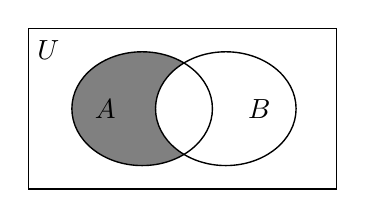
\begin{tikzpicture}[scale=0.85,line width=0.5pt]
\draw (0,0) rectangle (4.6,2.4);
\fill[gray] (1.7,1.2) ellipse (1.05 and 0.85);
\fill[white] (2.95,1.2) ellipse (1.05 and 0.85);
\draw (1.7,1.2) ellipse (1.05 and 0.85);
\draw (2.95,1.2) ellipse (1.05 and 0.85);
\node at (1.15,1.2) {$A$};
\node at (3.45,1.2) {$B$};
\node at (0.3,2.08) {$U$};
\end{tikzpicture}
\end{center}

\ifanswer
\solbegin
\step{$A=\{x\mid y=\sqrt{-x^2+x+2}\}=\{x\mid-1\leqslant x\leqslant2\}$，}
\step{$\overline B=\{x\mid 0\leqslant x\leqslant5\}$，$C=A\cap\overline B=[0,2]$.}
\solend
\fi

\item 关于 $x$ 的不等式 $ax-b<0$ 的解集为 $(2,+\infty)$，则关于 $x$ 的不等式 $(ax+b)(x-1)<0$ 的解集为\blankline[4.4em].

\ifanswer
\solbegin
\step{因为关于 $x$ 的不等式 $ax-b<0$ 的解集为 $(2,+\infty)$，所以 $\begin{cases}a<0\\2a-b=0\end{cases}$，}
\step{所以不等式 $(ax+b)(x-1)<0$ 可化为 $a\left(x+\dfrac ba\right)(x-1)<0$，$a<0$，}
\step{所以 $(x+2)(x-1)>0$，}
\step{所以所求解集为 $(-\infty,-2)\cup(1,+\infty)$.}
\solend
\fi

\item $a_1$、$b_1$、$a_2$、$b_2$ 均为非零实数，不等式 $a_1x+b_1>0$ 和 $a_2x+b_2>0$ 的解集分别为集合 $M$、$N$，那么“$\dfrac{a_1}{a_2}=\dfrac{b_1}{b_2}$”是“$M=N$”的\blankline[4.4em]条件（选填“充分非必要”、“必要非充分”、“充要”和“既非充分也非必要”）.

\ifanswer
\solbegin
\step{当 $a_1=b_1=1$，$a_2=b_2=-1$ 时，满足 $\dfrac{a_1}{a_2}=\dfrac{b_1}{b_2}$，}
\step{但是 $M=N$ 不成立，即充分性不成立；}
\step{若 $M=N$ 时，$\dfrac{a_1}{a_2}=\dfrac{b_1}{b_2}$ 一定成立，即必要性成立.}
\step{故为必要不充分条件.}% 原卷选项列“必要非充分”、解析结论作“必要不充分”，照录
\solend
\fi

\item 已知集合 $\{a,b,c\}=\{0,1,2\}$，且下列三个关系：① $a\neq2$；② $b=2$；③ $c\neq0$；有且只有一个正确，则 $100a+10b+c=$\blankline[4.4em].

\ifanswer
\solbegin
\step{列表如下：}
\begin{center}
\begin{tabular}{|c|c|c|c|c|}
\hline
 & ① & ② & ③ & \\
\hline
① 正确 & $a\neq2$ & $b\neq2$ & $c=0$ & 无解\\
\hline
② 正确 & $a=2$ & $b=2$ & $c=0$ & 矛盾\\
\hline
③ 正确 & $a=2$ & $b\neq2$ & $c\neq0$ & $a=2,b=0,c=1$\\
\hline
\end{tabular}
\end{center}
\step{所以 $100a+10b+c=201$.}
\solend
\fi

\end{enumerate}

\bigsec{二、选择题}

\begin{enumerate}
\setcounter{enumi}{12}

\item 已知 $a$,$b$,$c\in\R$,$b>c$，则下列不等式中恒成立的是\mbox{（\quad）}

\keepwithprev
A. $a+b^2>a+c^2$\qquad\quad B. $a^2+b>a^2+c$\qquad\quad C. $ab^2>ac^2$\qquad\quad D. $a^2b>a^2c$

\ifanswer
\solbegin
\step{对于 $A$，取 $b=1,c=-1$，错误；对于 $B$，由不等式的同向可加性得正确；}
\step{对于 $C$，取 $a=1,b=1,c=-2$，错误；对于 $D$，取 $a=0$，错误；}
\step{故选 $B$.}
\solend
\fi

\item 给出命题：“如果 $n$ 是素数，那么 $n^2+2$ 不是素数”，甲同学判断该命题是假命题，他做出这个判断的反例可以是\mbox{（\quad）}% 原卷把答案“$B$”印在题干括号内、无【解析】

\keepwithprev
A. $n=2$\qquad\quad B. $n=3$\qquad\quad C. $n=4$\qquad\quad D. $n=5$

\ifanswer
\ans{$B$}
\fi

\item 设集合 $A=\left\{x\,\middle\vert\,x=\dfrac n2,n\in\Z\right\}$，$B=\left\{x\,\middle\vert\,x=n+\dfrac12,n\in\Z\right\}$，则下列图形能表示 $A$ 与 $B$ 关系的是\mbox{（\quad）}

\keepwithprev
\begin{center}
% 原卷四个文氏图选项按原图形状用 TikZ 重排。
\begin{tabular}{c@{\qquad\qquad}c}
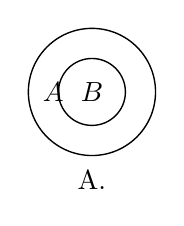
\begin{tikzpicture}[scale=0.85,line width=0.5pt]
\draw (0.9,0.9) circle (0.95);
\draw (0.9,0.9) circle (0.5);
\node at (0.32,0.9) {$A$};
\node at (0.9,0.9) {$B$};
\node[anchor=north] at (0.9,-0.12) {A.};
\end{tikzpicture}
&
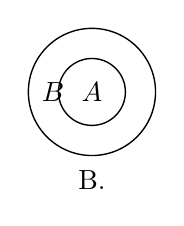
\begin{tikzpicture}[scale=0.85,line width=0.5pt]
\draw (0.9,0.9) circle (0.95);
\draw (0.9,0.9) circle (0.5);
\node at (0.32,0.9) {$B$};
\node at (0.9,0.9) {$A$};
\node[anchor=north] at (0.9,-0.12) {B.};
\end{tikzpicture}
\\[12pt]
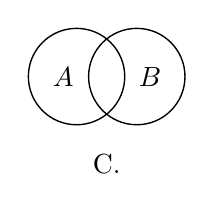
\begin{tikzpicture}[scale=0.85,line width=0.5pt]
\draw (0.65,0.9) circle (0.72);
\draw (1.55,0.9) circle (0.72);
\node at (0.45,0.9) {$A$};
\node at (1.75,0.9) {$B$};
\node[anchor=north] at (1.1,-0.12) {C.};
\end{tikzpicture}
&
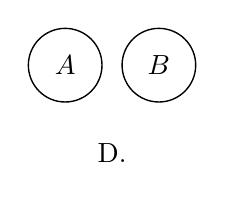
\begin{tikzpicture}[scale=0.85,line width=0.5pt]
\draw (0.55,0.9) circle (0.55);
\draw (1.95,0.9) circle (0.55);
\node at (0.55,0.9) {$A$};
\node at (1.95,0.9) {$B$};
\node[anchor=north] at (1.25,-0.12) {D.};
\end{tikzpicture}
\end{tabular}
\end{center}

\ifanswer
\solbegin
\step{$B\subset A$，图形能表示 $A$ 与 $B$ 关系的是 $A$. 故选 $A$.}
\solend
\fi

\item 以某些整数为元素的集合 $P$ 具有以下性质：

（1）$P$ 中元素有正数，也有负数；（2）$P$ 中元素有奇数，也有偶数；

（3）$-1\notin P$；（4）若 $x$、$y\in P$，则 $x+y\in P$.

则下列选项哪个是正确的\mbox{（\quad）}

\keepwithprev
A. 集合 $P$ 中一定有 $0$ 但没有 $2$\qquad\qquad B. 集合 $P$ 中一定有 $0$ 可能有 $2$

C. 集合 $P$ 中可能有 $0$ 可能有 $2$\qquad\qquad D. 集合 $P$ 中既没有 $0$ 又没有 $2$

\ifanswer
\solbegin
\step{由（4）得 $x\in P$，则 $kx\in P(k$ 是正整数$)$.}
\step{由（1）可设 $x$、$y\in P$，且 $x>0$，$y<0$，则 $xy$、$(-y)x\in P$，}
\step{因而 $0=xy+(-y)x\in P$.}
\step{假设 $2\in P$，则 $2k\in P$. 由上面及（4）得 $0$，$2$，$4$，$6$，$8$，$\cdots$ 均在 $P$ 中，}
\step{故 $2k-2\in P(k$ 是正整数$)$，}
\step{不妨令 $P$ 中负数为奇数 $-2k+1(k$ 为正整数$)$，}
\step{由（4）得 $(2k-2)+(-2k+1)=-1\in P$，矛盾.}
\step{故若 $2\in P$，则 $P$ 中没有负奇数.}
\step{若 $P$ 中负数为偶数，设为 $-2k(k$ 为正整数$)$，则由（4）及 $2\in P$，}
\step{得 $-2$,$-4$,$-6$,$\cdots$ 均在 $P$ 中，即 $-2m-2\in P(m$ 为非负整数$)$，}
\step{则 $P$ 中正奇数为 $2m+1$，由（4）得 $(-2m-2)+(2m+1)=-1\in P$，矛盾.}
\step{综上，$0\in P$，$2\notin P$，故选 $A$.}
\solend
\fi

\end{enumerate}

\bigsec{三、解答题}

\begin{enumerate}
\setcounter{enumi}{16}

\item （1）已知 $a$、$b$ 为实数，比较 $a^2+b^2$ 与 $4a-2b-5$ 的值的大小.

（2）若 $-1\leqslant x+y\leqslant2$，$-2\leqslant x-y\leqslant1$，求 $x-2y$ 的范围.

\ifanswer
\solbegin
\step{（1）$a^2+b^2-(4a-2b-5)=a^2-4a+4+b^2+2b+1=(a-2)^2+(b+1)^2\geqslant0$，}
\step{故 $a^2+b^2\geqslant4a-2b-5$.}
\step{（2）设 $x-2y=m(x+y)+n(x-y)$，则 $x-2y=(m+n)x+(m-n)y$，}
\step{所以 $\begin{cases}m+n=1\\m-n=-2\end{cases}$，解得 $n=\dfrac32$，$m=-\dfrac12$，}
\step{所以 $x-2y=-\dfrac12(x+y)+\dfrac32(x-y)$，}
\step{因为 $-1\leqslant x+y\leqslant2$，$-2\leqslant x-y\leqslant1$，}
\step{所以 $-1\leqslant-\dfrac12(x+y)\leqslant\dfrac12$，$-3\leqslant\dfrac32(x-y)\leqslant\dfrac32$，}
\step{所以 $-4\leqslant-\dfrac12(x+y)+\dfrac32(x-y)\leqslant2$，即 $-4\leqslant x-2y\leqslant2$，}
\step{故 $x-2y$ 的范围是 $[-4,2]$.}
\solend
\fi

\item 已知集合 $A=\{x\mid\lvert x-2\rvert<a\}$，集合 $B=\left\{x\,\middle\vert\,\dfrac{2x-1}{x+2}<1\right\}$.

（1）若 $a=2$，求 $A\cup B$,$A\cap B$；

（2）若 $A\cap B=A$，求实数 $a$ 的取值范围.

\ifanswer
\solbegin
\step{（1）由题意得 $A=(0,4)$,$B=(-2,3)$，所以 $A\cup B=(-2,4)$,$A\cap B=(0,3)$；}
\step{（2）因为 $A\cap B=A$，所以 $A\subseteq B$，}
\step{当 $a\leqslant0$ 时，$A=\varnothing$，满足 $A\subseteq B$；}
\step{当 $a>0$ 时，$A=(2-a,2+a)$,$B=(-2,3)$，}
\step{因为 $A\subseteq B$，所以 $\begin{cases}-2\leqslant2-a\\3\geqslant2+a\end{cases}$，解得 $a\leqslant1$，即 $0<a\leqslant1$.}
\step{因此，实数 $a$ 的取值范围为 $(-\infty,1]$.}
\solend
\fi

\item 我校校园文化节即将到来，高一年级将开展“数字配对”的抽奖活动，活动规则如下：每人可以抽取一张卡片，每张卡片上都印有一个不小于 $-10$ 且不大于 $10$ 的整数，其中不含 $2$. 每张卡片数字对应一个抽奖号码，卡片上的数字减去 $2$ 所得的差，与抽奖号码减去 $3$ 所得的差，两者的乘积等于 $12$.

（1）记卡片上的数字为 $x$，卡片数字对应的抽奖号码为 $y$，请用含有卡片数字 $x$ 的式子来表示抽奖号码 $y$；

（2）当抽奖号码不小于 $3$ 且不大于 $7$ 时，抽奖者可以领取奖品. 请问抽到哪些数字的卡片可以领取奖品？请写出满足领取奖品的卡片数字所组成的集合.

\ifanswer
\solbegin
\step{（1）卡片上的数字为 $x$，对应的抽奖号码为 $y$，}
\step{由题意得 $(x-2)(y-3)=12$，因为 $x\neq2$，所以 $y=3+\dfrac{12}{x-2}$，}
\step{所以 $y=3+\dfrac{12}{x-2}(-10\leqslant x\leqslant10,x\in\Z,x\neq2)$.}
\step{（2）由（1）得 $y=3+\dfrac{12}{x-2}(-10\leqslant x\leqslant10,x\in\Z,x\neq2)$，}
\step{由抽奖条件，得 $3\leqslant3+\dfrac{12}{x-2}\leqslant7$，$x\geqslant5$，所以 $5\leqslant x\leqslant10$，$x\in\Z$，}
\step{所以可领取奖品的卡片数字为 $\{5,6,7,8,9,10\}$.}
\solend
\fi

\item （1）已知 $m\in\R$，若不等式 $(m+1)x^2-mx+m-1<0$ 的解集是空集，求 $m$ 的取值范围；

（2）命题 $P:x^2-5x+6<0$，命题 $q:x^2-4ax+3a^2<0$，若命题 $P$ 是命题 $q$ 的充分非必要条件，求实数 $a$ 的取值范围.

\ifanswer
\solbegin
\step{（1）①当 $m+1=0$，即 $m=-1$ 时，$f(x)=x-2$，不合题意；}
\step{②当 $m+1\neq0$，即 $m\neq-1$ 时，$\begin{cases}m+1>0\\\Delta=m^2-4(m+1)(m-1)\leqslant0\end{cases}$，解得 $m\geqslant\dfrac{2\sqrt3}{3}$，}
\step{所以 $m$ 的取值范围是 $\left[\dfrac{2\sqrt3}{3},+\infty\right)$；}
\step{（2）解 $x^2-5x+6<0$，因式分解得 $(x-2)(x-3)<0$，故 $P$ 的解集为 $(2,3)$，}
\step{解 $x^2-4ax+3a^2<0$，因式分解得 $(x-a)(x-3a)<0$，}
\step{因为命题 $P$ 是命题 $q$ 的充分不必要条件，所以 $(2,3)$ 是 $q$ 解集的真子集，}
\step{当 $a=0$ 时，$q$ 的解集为 $\varnothing$，不合题意，舍去；}
\step{当 $a<0$ 时，$q$ 的解集为 $(3a,a)$，$\begin{cases}3a\leqslant2\\a\geqslant3\end{cases}$，不等式组无解，舍去；}
\step{当 $a>0$ 时，$q$ 的解集为 $(a,3a)$，又因为 $(2,3)$ 是 $q$ 解集的真子集，}
\step{所以 $\begin{cases}a\leqslant2\\3a\geqslant3\end{cases}$（等号不同时取），解得 $1\leqslant a\leqslant2$；}
\step{综上，实数 $a$ 的取值范围是 $[1,2]$.}
\solend
\fi

\item 对于至少含两个元素的有限正整数集 $A$，定义它的“两两和集”为
$S(A)=\{z\mid z=x+y$，其中 $x$、$y\in A$，且 $x<y\}$.

（1）若 $A=\{1,2,4,5\}$，求 $S(A)$；

（2）已知集合 $A$ 中恰好含有四个元素，且 $S(A)=\{5,7,8,10,11,13\}$，写出所有符合条件的集合 $A$；

（3）猜想：当集合 $A$ 含有 $n$ 个元素（$n\geqslant2$）时，$S(A)$ 的元素个数最少是多少？证明你的猜想.

\ifanswer
\solbegin
\step{（1）因为 $A=\{1,2,4,5\}$，计算所有两两和并去掉重复的结果有 $3$，$5$，$6$，$7$，$9$，}
\step{所以 $S(A)=\{3,5,6,7,9\}$.}
\step{（2）设 $A=\{a,b,c,d\}$，其中 $a<b<c<d$，且 $S(A)=\{5,7,8,10,11,13\}$，}
\step{四个元素共有六种两两配对，和集恰好有六个元素，}
\step{因此六个和互不相同.}
\step{这六个数分别为 $a+b$,$a+c$,$a+d$,$b+c$,$b+d$,$c+d$，}
\step{所以这六个数从小到大，可以确定第一个数为 $a+b$，第二数为 $a+c$，}
\step{第五个数为 $b+d$，第六数为 $c+d$，}
\step{第三个数和第四个数不能确定，即 $b+c$ 和 $a+d$ 的大小不定.}
\step{所以 $a+b=5$,$a+c=7$,$b+d=11$,$c+d=13$.}
\step{由此得到 $b=5-a$,$c=7-a$,$d=6+a$，}
\step{于是 $a+d=2a+6$,$b+c=12-2a$.}
\step{其余两个数 $b+c$,$a+d$ 对应 $8$,$10$，分两种情况讨论：}
\step{①若 $b+c=8$,$a+d=10$，则 $\begin{cases}12-2a=8\\2a+6=10\end{cases}$，解得 $a=2$，}
\step{所以 $A=\{2,3,5,8\}$；}
\step{②若 $b+c=10$,$a+d=8$，则 $\begin{cases}12-2a=10\\2a+6=8\end{cases}$，解得 $a=1$，}
\step{所以 $A=\{1,4,6,7\}$；}
\step{检验得，两组均符合题意.}
\step{因此所有符合条件的集合为 $A=\{1,4,6,7\}$ 或 $A=\{2,3,5,8\}$.}
\step{（3）猜想：两两和集的元素个数的最小值为 $2n-3$. 证明如下：}
\step{将集合中的元素按从小到大排列为 $a_1<a_2<\cdots<a_n$，}
\step{当 $n=2$ 时，两两和集恰好有一个元素，结论成立.}
\step{当 $n\geqslant3$ 时，考虑下列均属于 $S(A)$ 的数，}
\step{由不等式的传递性得严格不等式：}
\step{$a_1+a_2<a_1+a_3<\cdots<a_1+a_n<a_2+a_n<\cdots<a_{n-1}+a_n$，}
\step{其中 $a_1+a_2<a_1+a_3<\cdots<a_1+a_n$ 共有 $n-1$ 个不相等的数；}
\step{$a_2+a_n<\cdots<a_{n-1}+a_n$ 共有 $n-2$ 个不相等的数，}
\step{所以一共有 $(n-1)+(n-2)=2n-3$ 个，}
\step{因此，两两和集至少含有 $2n-3$ 个元素.}
\step{再证明可以取到 $2n-3$：}
\step{对任意 $n\geqslant2$，取 $A=\{1,2,\cdots,n\}$，}
\step{所有两两和都是不小于 $3$ 且不大于 $2n-1$ 的整数，}
\step{其中，$1+2$,$1+3$,$\cdots$,$1+n$ 是从 $3$ 到 $n+1$ 的整数；}
\step{当 $n\geqslant3$ 时，$2+n$,$3+n$,$\cdots$,$(n-1)+n$ 可取到其余整数；}
\step{因此 $S(A)=\{3,4,\cdots,2n-1\}$，其元素个数为 $(2n-1)-3+1=2n-3$，}
\step{所以所求最小值为 $2n-3$.}
\solend
\fi

\end{enumerate}

\end{document}
"
% 紧凑版：xelatex "\def\iscompact{1}% 高一118_罗店中学_10月月考.tex
%   —— 高一上数学“2026-2027 年罗店中学高一上 10 月月考”（试卷版/答案版）
% 试卷版：xelatex 高一118_罗店中学_10月月考.tex
% 答案版：xelatex "\def\isanswer{1}\input{高一118_罗店中学_10月月考.tex}"
% 紧凑版：xelatex "\def\iscompact{1}\input{高一118_罗店中学_10月月考.tex}"
%
% 原始材料：微信公众号“魔都数学加油站”文章，作者破晓，2026-11-06 17:58 发布；
% 连载“27学年高一118”，原文标题“27学年高一118——2026-2027年上海市罗店中学高一上10月月考”；
% 原文链接：https://mp.weixin.qq.com/s/4edo8awYdjmWJl153X-aDA。
% 正文为 9 张 PNG 页（第 2、3、5、9 页 2560×3620，其余 4762×6735），
% 题目下印有【解析】或【答案】，为讲评版。
% 题目、解析均据原图转录；卷面红色水印及公众号页脚未录入。
%
% 卷首标题：原卷印作“2026-2027 年罗店中学高一上 10 月月考”（公众号标题中的“上海市”
% 卷面标题行没有，本稿照卷面），年份区间按全稿惯例排 en dash；原卷未印副标题，本稿按题目内容
% 标为“集合与常用逻辑用语、不等式”。
%
% 与原卷的排版差异：
%   ① 原文从第 3 题起，填空题 3—12、选择题 13—16、解答题 17—21，共 19 题，本稿保留原题号；
%   ② 原卷每题下直接印【解析】／【答案】，本稿按全稿惯例置于答案版；第 4 题只印【答案】、
%      第 14 题把答案“$B$”印在题干括号内且无【解析】，均另提 \ans{}；其余选择题答案在
%      解析末句“故选 …”，括号内留空；
%   ③ 原卷未印副标题，本稿按“知识模块”口径补出；
%   ④ 原卷填空横线按全稿惯例排为 \blankline[4.4em]；选择题括号排 \mbox{（\quad）}、
%      选项段前按惯例加 \keepwithprev；解答题不留作答区（原卷为讲评版，与 109—117 同）；
%   ⑤ 原卷数集 $R$／$Z$ 按全稿惯例改 \R、\Z，补集照原卷上划线排 \overline{B}。
%
% 子集符号：第 6 题、第 18 题的 $\{x\mid x<1\}\subseteq\{x\mid x<3a-2\}$ 与 $A\subseteq B$
%   印有下划线，照录 \subseteq；第 15 题解析的 $B\subset A$ 印单线（真子集、无下划线），
%   按 18／96 成例照录 \subset。
%
% 判别式字形：第 20 题 (1) cases 的判别式原卷排 $\Delta$（等腰、右厚），照录 \Delta。
%
% 图与表：第 9 题题干的文氏图（矩形 $U$ 内两椭圆 $A$、$B$，阴影为 $A\cap\overline B$）
%   按原图形状用 TikZ 重绘（三版都出）；第 12 题解析的“列表”按原卷用 tabular 重排
%   （仅答案版）；第 15 题四个文氏图选项按原图形状用 TikZ 重排（三版都出）。
%
% 原卷存疑照录：第 8 题解析“$2022+3\cdot1\cdot(-1)=2026$”一行、第 11 题解析结论
%   作“必要不充分条件”而选项列“必要非充分”、第 20 题 (2) 的 cases，均照录加注。
%
% 行数核对：逐题数 \step/\stepm 条数，合计 110 条（Q3：2；Q4：0；Q5：1；Q6：2；Q7：5；
% Q8：3；Q9：2；Q10：4；Q11：4；Q12：2；Q13：3；Q14：0；Q15：1；Q16：12；Q17：9；
% Q18：6；Q19：6；Q20：11；Q21：36），与原卷印刷行逐题相等（cases／tabular／TikZ
% 图块作一个印刷行计）。第 4 题只印【答案】、第 14 题括号内印答案且无解析，均提 \ans{}，
% 不计入 \step 账。
%
\documentclass[a4paper,11pt]{article}
\usepackage{common}

\begin{document}

\examtitlest[3]{2026--2027 年罗店中学高一上 10 月月考}{集合与常用逻辑用语、不等式}

\bigsec{一、填空题}

\begin{enumerate}
\setcounter{enumi}{2}

\item 若 $2x^2+3x+5=a(2x+1)(x+1)+b$ 恒成立，则 $a-b$ 的值\blankline[4.4em].

\ifanswer
\solbegin
\step{因为 $2x^2+3x+5=a(2x+1)(x+1)+b=2ax^2+3ax+a+b$ 恒成立，}
\step{所以 $\begin{cases}2=2a\\3=3a\\5=a+b\end{cases}$，所以 $\begin{cases}a=1\\b=4\end{cases}$，故 $a-b$ 的值为 $-3$.}
\solend
\fi

\item “$a$、$b$ 中至少有一个能被 $6$ 整除”的否定形式是\blankline[4.4em].

\ifanswer
\ans{$a$、$b$ 都不能被 $6$ 整除}
\fi

\item 设集合 $A=\{1,2\}$，则满足 $A\cup B=\{1,2,3\}$ 的集合 $B$ 的个数是\blankline[4.4em].

\ifanswer
\solbegin
\step{$B=\{3\}$,$\{1,3\}$,$\{2,3\}$,$\{1,2,3\}$，个数为 $4$.}
\solend
\fi

\item 命题“若 $x<1$，则 $x<3a-2$”是真命题，求实数 $a$ 的取值范围是\blankline[4.4em].

\ifanswer
\solbegin
\step{$\alpha:x<1$,$\beta:x<3a-2$，且若 $\alpha$ 则 $\beta$ 是真命题，}
\step{则 $\{x\mid x<1\}\subseteq\{x\mid x<3a-2\}$，所以 $3a-2\geqslant1$，解得 $a\geqslant1$.}
\solend
\fi

\item 不论实数 $m$ 取什么值，点 $P(m+1,2-m)$ 一定不在第\blankline[4.4em]象限（选填“一”、“二”、“三”或“四”）.

\ifanswer
\solbegin
\step{当 $m+1>0$，$2-m>0$ 时，解得 $-1<m<2$，此时点 $P$ 在第一象限；}
\step{当 $m+1<0$，$2-m>0$ 时，解得 $m<-1$，此时点 $P$ 在第二象限；}
\step{当 $m+1<0$，$2-m<0$ 时，$m$ 无解，此时点 $P$ 不可能在第三象限；}
\step{当 $m+1>0$，$2-m<0$ 时，解得 $m>2$，此时点 $P$ 在第四象限.}
\step{故一定不在第三象限.}
\solend
\fi

\item 设 $x_1$、$x_2$ 是方程 $x^2+x-3=0$ 的两个实数根，则 $x_1^2-x_2+2022=$\blankline[4.4em].

\ifanswer
\solbegin
\step{$x_1$、$x_2$ 是方程 $x^2+x-3=0$ 的两个实数根，}
\step{得 $x_1+x_2=-1$，$x_1^2+x_1-3=0$，所以 $x_1^2=3-x_1$，}
\step{$x_1^2-x_2+2022=3-x_1-x_2+2022=2022+3\cdot1\cdot(-1)=2026$.}
\solend
\fi

\item 如图，已知全集 $U=\R$，集合 $A=\{x\mid y=\sqrt{-x^2+x+2}\}$，$B=\{x\mid x<0$ 或 $x>5\}$. 集合 $C$ 表示图中阴影区域对应的集合，则集合 $C=$\blankline[4.4em]（用区间表示）.

\begin{center}
% 原卷文氏图：矩形 U 内两椭圆 A（阴影）、B，阴影为 A\cap\overline B，按原图形状用 TikZ 重绘。
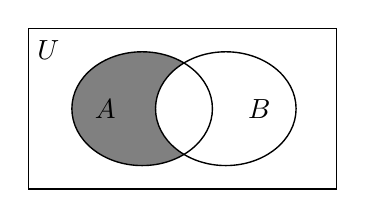
\begin{tikzpicture}[scale=0.85,line width=0.5pt]
\draw (0,0) rectangle (4.6,2.4);
\fill[gray] (1.7,1.2) ellipse (1.05 and 0.85);
\fill[white] (2.95,1.2) ellipse (1.05 and 0.85);
\draw (1.7,1.2) ellipse (1.05 and 0.85);
\draw (2.95,1.2) ellipse (1.05 and 0.85);
\node at (1.15,1.2) {$A$};
\node at (3.45,1.2) {$B$};
\node at (0.3,2.08) {$U$};
\end{tikzpicture}
\end{center}

\ifanswer
\solbegin
\step{$A=\{x\mid y=\sqrt{-x^2+x+2}\}=\{x\mid-1\leqslant x\leqslant2\}$，}
\step{$\overline B=\{x\mid 0\leqslant x\leqslant5\}$，$C=A\cap\overline B=[0,2]$.}
\solend
\fi

\item 关于 $x$ 的不等式 $ax-b<0$ 的解集为 $(2,+\infty)$，则关于 $x$ 的不等式 $(ax+b)(x-1)<0$ 的解集为\blankline[4.4em].

\ifanswer
\solbegin
\step{因为关于 $x$ 的不等式 $ax-b<0$ 的解集为 $(2,+\infty)$，所以 $\begin{cases}a<0\\2a-b=0\end{cases}$，}
\step{所以不等式 $(ax+b)(x-1)<0$ 可化为 $a\left(x+\dfrac ba\right)(x-1)<0$，$a<0$，}
\step{所以 $(x+2)(x-1)>0$，}
\step{所以所求解集为 $(-\infty,-2)\cup(1,+\infty)$.}
\solend
\fi

\item $a_1$、$b_1$、$a_2$、$b_2$ 均为非零实数，不等式 $a_1x+b_1>0$ 和 $a_2x+b_2>0$ 的解集分别为集合 $M$、$N$，那么“$\dfrac{a_1}{a_2}=\dfrac{b_1}{b_2}$”是“$M=N$”的\blankline[4.4em]条件（选填“充分非必要”、“必要非充分”、“充要”和“既非充分也非必要”）.

\ifanswer
\solbegin
\step{当 $a_1=b_1=1$，$a_2=b_2=-1$ 时，满足 $\dfrac{a_1}{a_2}=\dfrac{b_1}{b_2}$，}
\step{但是 $M=N$ 不成立，即充分性不成立；}
\step{若 $M=N$ 时，$\dfrac{a_1}{a_2}=\dfrac{b_1}{b_2}$ 一定成立，即必要性成立.}
\step{故为必要不充分条件.}% 原卷选项列“必要非充分”、解析结论作“必要不充分”，照录
\solend
\fi

\item 已知集合 $\{a,b,c\}=\{0,1,2\}$，且下列三个关系：① $a\neq2$；② $b=2$；③ $c\neq0$；有且只有一个正确，则 $100a+10b+c=$\blankline[4.4em].

\ifanswer
\solbegin
\step{列表如下：}
\begin{center}
\begin{tabular}{|c|c|c|c|c|}
\hline
 & ① & ② & ③ & \\
\hline
① 正确 & $a\neq2$ & $b\neq2$ & $c=0$ & 无解\\
\hline
② 正确 & $a=2$ & $b=2$ & $c=0$ & 矛盾\\
\hline
③ 正确 & $a=2$ & $b\neq2$ & $c\neq0$ & $a=2,b=0,c=1$\\
\hline
\end{tabular}
\end{center}
\step{所以 $100a+10b+c=201$.}
\solend
\fi

\end{enumerate}

\bigsec{二、选择题}

\begin{enumerate}
\setcounter{enumi}{12}

\item 已知 $a$,$b$,$c\in\R$,$b>c$，则下列不等式中恒成立的是\mbox{（\quad）}

\keepwithprev
A. $a+b^2>a+c^2$\qquad\quad B. $a^2+b>a^2+c$\qquad\quad C. $ab^2>ac^2$\qquad\quad D. $a^2b>a^2c$

\ifanswer
\solbegin
\step{对于 $A$，取 $b=1,c=-1$，错误；对于 $B$，由不等式的同向可加性得正确；}
\step{对于 $C$，取 $a=1,b=1,c=-2$，错误；对于 $D$，取 $a=0$，错误；}
\step{故选 $B$.}
\solend
\fi

\item 给出命题：“如果 $n$ 是素数，那么 $n^2+2$ 不是素数”，甲同学判断该命题是假命题，他做出这个判断的反例可以是\mbox{（\quad）}% 原卷把答案“$B$”印在题干括号内、无【解析】

\keepwithprev
A. $n=2$\qquad\quad B. $n=3$\qquad\quad C. $n=4$\qquad\quad D. $n=5$

\ifanswer
\ans{$B$}
\fi

\item 设集合 $A=\left\{x\,\middle\vert\,x=\dfrac n2,n\in\Z\right\}$，$B=\left\{x\,\middle\vert\,x=n+\dfrac12,n\in\Z\right\}$，则下列图形能表示 $A$ 与 $B$ 关系的是\mbox{（\quad）}

\keepwithprev
\begin{center}
% 原卷四个文氏图选项按原图形状用 TikZ 重排。
\begin{tabular}{c@{\qquad\qquad}c}
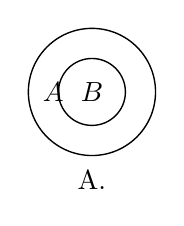
\begin{tikzpicture}[scale=0.85,line width=0.5pt]
\draw (0.9,0.9) circle (0.95);
\draw (0.9,0.9) circle (0.5);
\node at (0.32,0.9) {$A$};
\node at (0.9,0.9) {$B$};
\node[anchor=north] at (0.9,-0.12) {A.};
\end{tikzpicture}
&
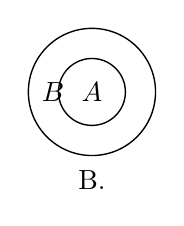
\begin{tikzpicture}[scale=0.85,line width=0.5pt]
\draw (0.9,0.9) circle (0.95);
\draw (0.9,0.9) circle (0.5);
\node at (0.32,0.9) {$B$};
\node at (0.9,0.9) {$A$};
\node[anchor=north] at (0.9,-0.12) {B.};
\end{tikzpicture}
\\[12pt]
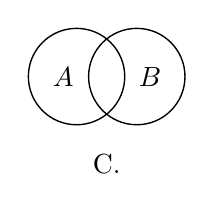
\begin{tikzpicture}[scale=0.85,line width=0.5pt]
\draw (0.65,0.9) circle (0.72);
\draw (1.55,0.9) circle (0.72);
\node at (0.45,0.9) {$A$};
\node at (1.75,0.9) {$B$};
\node[anchor=north] at (1.1,-0.12) {C.};
\end{tikzpicture}
&
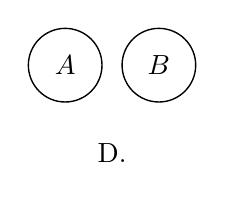
\begin{tikzpicture}[scale=0.85,line width=0.5pt]
\draw (0.55,0.9) circle (0.55);
\draw (1.95,0.9) circle (0.55);
\node at (0.55,0.9) {$A$};
\node at (1.95,0.9) {$B$};
\node[anchor=north] at (1.25,-0.12) {D.};
\end{tikzpicture}
\end{tabular}
\end{center}

\ifanswer
\solbegin
\step{$B\subset A$，图形能表示 $A$ 与 $B$ 关系的是 $A$. 故选 $A$.}
\solend
\fi

\item 以某些整数为元素的集合 $P$ 具有以下性质：

（1）$P$ 中元素有正数，也有负数；（2）$P$ 中元素有奇数，也有偶数；

（3）$-1\notin P$；（4）若 $x$、$y\in P$，则 $x+y\in P$.

则下列选项哪个是正确的\mbox{（\quad）}

\keepwithprev
A. 集合 $P$ 中一定有 $0$ 但没有 $2$\qquad\qquad B. 集合 $P$ 中一定有 $0$ 可能有 $2$

C. 集合 $P$ 中可能有 $0$ 可能有 $2$\qquad\qquad D. 集合 $P$ 中既没有 $0$ 又没有 $2$

\ifanswer
\solbegin
\step{由（4）得 $x\in P$，则 $kx\in P(k$ 是正整数$)$.}
\step{由（1）可设 $x$、$y\in P$，且 $x>0$，$y<0$，则 $xy$、$(-y)x\in P$，}
\step{因而 $0=xy+(-y)x\in P$.}
\step{假设 $2\in P$，则 $2k\in P$. 由上面及（4）得 $0$，$2$，$4$，$6$，$8$，$\cdots$ 均在 $P$ 中，}
\step{故 $2k-2\in P(k$ 是正整数$)$，}
\step{不妨令 $P$ 中负数为奇数 $-2k+1(k$ 为正整数$)$，}
\step{由（4）得 $(2k-2)+(-2k+1)=-1\in P$，矛盾.}
\step{故若 $2\in P$，则 $P$ 中没有负奇数.}
\step{若 $P$ 中负数为偶数，设为 $-2k(k$ 为正整数$)$，则由（4）及 $2\in P$，}
\step{得 $-2$,$-4$,$-6$,$\cdots$ 均在 $P$ 中，即 $-2m-2\in P(m$ 为非负整数$)$，}
\step{则 $P$ 中正奇数为 $2m+1$，由（4）得 $(-2m-2)+(2m+1)=-1\in P$，矛盾.}
\step{综上，$0\in P$，$2\notin P$，故选 $A$.}
\solend
\fi

\end{enumerate}

\bigsec{三、解答题}

\begin{enumerate}
\setcounter{enumi}{16}

\item （1）已知 $a$、$b$ 为实数，比较 $a^2+b^2$ 与 $4a-2b-5$ 的值的大小.

（2）若 $-1\leqslant x+y\leqslant2$，$-2\leqslant x-y\leqslant1$，求 $x-2y$ 的范围.

\ifanswer
\solbegin
\step{（1）$a^2+b^2-(4a-2b-5)=a^2-4a+4+b^2+2b+1=(a-2)^2+(b+1)^2\geqslant0$，}
\step{故 $a^2+b^2\geqslant4a-2b-5$.}
\step{（2）设 $x-2y=m(x+y)+n(x-y)$，则 $x-2y=(m+n)x+(m-n)y$，}
\step{所以 $\begin{cases}m+n=1\\m-n=-2\end{cases}$，解得 $n=\dfrac32$，$m=-\dfrac12$，}
\step{所以 $x-2y=-\dfrac12(x+y)+\dfrac32(x-y)$，}
\step{因为 $-1\leqslant x+y\leqslant2$，$-2\leqslant x-y\leqslant1$，}
\step{所以 $-1\leqslant-\dfrac12(x+y)\leqslant\dfrac12$，$-3\leqslant\dfrac32(x-y)\leqslant\dfrac32$，}
\step{所以 $-4\leqslant-\dfrac12(x+y)+\dfrac32(x-y)\leqslant2$，即 $-4\leqslant x-2y\leqslant2$，}
\step{故 $x-2y$ 的范围是 $[-4,2]$.}
\solend
\fi

\item 已知集合 $A=\{x\mid\lvert x-2\rvert<a\}$，集合 $B=\left\{x\,\middle\vert\,\dfrac{2x-1}{x+2}<1\right\}$.

（1）若 $a=2$，求 $A\cup B$,$A\cap B$；

（2）若 $A\cap B=A$，求实数 $a$ 的取值范围.

\ifanswer
\solbegin
\step{（1）由题意得 $A=(0,4)$,$B=(-2,3)$，所以 $A\cup B=(-2,4)$,$A\cap B=(0,3)$；}
\step{（2）因为 $A\cap B=A$，所以 $A\subseteq B$，}
\step{当 $a\leqslant0$ 时，$A=\varnothing$，满足 $A\subseteq B$；}
\step{当 $a>0$ 时，$A=(2-a,2+a)$,$B=(-2,3)$，}
\step{因为 $A\subseteq B$，所以 $\begin{cases}-2\leqslant2-a\\3\geqslant2+a\end{cases}$，解得 $a\leqslant1$，即 $0<a\leqslant1$.}
\step{因此，实数 $a$ 的取值范围为 $(-\infty,1]$.}
\solend
\fi

\item 我校校园文化节即将到来，高一年级将开展“数字配对”的抽奖活动，活动规则如下：每人可以抽取一张卡片，每张卡片上都印有一个不小于 $-10$ 且不大于 $10$ 的整数，其中不含 $2$. 每张卡片数字对应一个抽奖号码，卡片上的数字减去 $2$ 所得的差，与抽奖号码减去 $3$ 所得的差，两者的乘积等于 $12$.

（1）记卡片上的数字为 $x$，卡片数字对应的抽奖号码为 $y$，请用含有卡片数字 $x$ 的式子来表示抽奖号码 $y$；

（2）当抽奖号码不小于 $3$ 且不大于 $7$ 时，抽奖者可以领取奖品. 请问抽到哪些数字的卡片可以领取奖品？请写出满足领取奖品的卡片数字所组成的集合.

\ifanswer
\solbegin
\step{（1）卡片上的数字为 $x$，对应的抽奖号码为 $y$，}
\step{由题意得 $(x-2)(y-3)=12$，因为 $x\neq2$，所以 $y=3+\dfrac{12}{x-2}$，}
\step{所以 $y=3+\dfrac{12}{x-2}(-10\leqslant x\leqslant10,x\in\Z,x\neq2)$.}
\step{（2）由（1）得 $y=3+\dfrac{12}{x-2}(-10\leqslant x\leqslant10,x\in\Z,x\neq2)$，}
\step{由抽奖条件，得 $3\leqslant3+\dfrac{12}{x-2}\leqslant7$，$x\geqslant5$，所以 $5\leqslant x\leqslant10$，$x\in\Z$，}
\step{所以可领取奖品的卡片数字为 $\{5,6,7,8,9,10\}$.}
\solend
\fi

\item （1）已知 $m\in\R$，若不等式 $(m+1)x^2-mx+m-1<0$ 的解集是空集，求 $m$ 的取值范围；

（2）命题 $P:x^2-5x+6<0$，命题 $q:x^2-4ax+3a^2<0$，若命题 $P$ 是命题 $q$ 的充分非必要条件，求实数 $a$ 的取值范围.

\ifanswer
\solbegin
\step{（1）①当 $m+1=0$，即 $m=-1$ 时，$f(x)=x-2$，不合题意；}
\step{②当 $m+1\neq0$，即 $m\neq-1$ 时，$\begin{cases}m+1>0\\\Delta=m^2-4(m+1)(m-1)\leqslant0\end{cases}$，解得 $m\geqslant\dfrac{2\sqrt3}{3}$，}
\step{所以 $m$ 的取值范围是 $\left[\dfrac{2\sqrt3}{3},+\infty\right)$；}
\step{（2）解 $x^2-5x+6<0$，因式分解得 $(x-2)(x-3)<0$，故 $P$ 的解集为 $(2,3)$，}
\step{解 $x^2-4ax+3a^2<0$，因式分解得 $(x-a)(x-3a)<0$，}
\step{因为命题 $P$ 是命题 $q$ 的充分不必要条件，所以 $(2,3)$ 是 $q$ 解集的真子集，}
\step{当 $a=0$ 时，$q$ 的解集为 $\varnothing$，不合题意，舍去；}
\step{当 $a<0$ 时，$q$ 的解集为 $(3a,a)$，$\begin{cases}3a\leqslant2\\a\geqslant3\end{cases}$，不等式组无解，舍去；}
\step{当 $a>0$ 时，$q$ 的解集为 $(a,3a)$，又因为 $(2,3)$ 是 $q$ 解集的真子集，}
\step{所以 $\begin{cases}a\leqslant2\\3a\geqslant3\end{cases}$（等号不同时取），解得 $1\leqslant a\leqslant2$；}
\step{综上，实数 $a$ 的取值范围是 $[1,2]$.}
\solend
\fi

\item 对于至少含两个元素的有限正整数集 $A$，定义它的“两两和集”为
$S(A)=\{z\mid z=x+y$，其中 $x$、$y\in A$，且 $x<y\}$.

（1）若 $A=\{1,2,4,5\}$，求 $S(A)$；

（2）已知集合 $A$ 中恰好含有四个元素，且 $S(A)=\{5,7,8,10,11,13\}$，写出所有符合条件的集合 $A$；

（3）猜想：当集合 $A$ 含有 $n$ 个元素（$n\geqslant2$）时，$S(A)$ 的元素个数最少是多少？证明你的猜想.

\ifanswer
\solbegin
\step{（1）因为 $A=\{1,2,4,5\}$，计算所有两两和并去掉重复的结果有 $3$，$5$，$6$，$7$，$9$，}
\step{所以 $S(A)=\{3,5,6,7,9\}$.}
\step{（2）设 $A=\{a,b,c,d\}$，其中 $a<b<c<d$，且 $S(A)=\{5,7,8,10,11,13\}$，}
\step{四个元素共有六种两两配对，和集恰好有六个元素，}
\step{因此六个和互不相同.}
\step{这六个数分别为 $a+b$,$a+c$,$a+d$,$b+c$,$b+d$,$c+d$，}
\step{所以这六个数从小到大，可以确定第一个数为 $a+b$，第二数为 $a+c$，}
\step{第五个数为 $b+d$，第六数为 $c+d$，}
\step{第三个数和第四个数不能确定，即 $b+c$ 和 $a+d$ 的大小不定.}
\step{所以 $a+b=5$,$a+c=7$,$b+d=11$,$c+d=13$.}
\step{由此得到 $b=5-a$,$c=7-a$,$d=6+a$，}
\step{于是 $a+d=2a+6$,$b+c=12-2a$.}
\step{其余两个数 $b+c$,$a+d$ 对应 $8$,$10$，分两种情况讨论：}
\step{①若 $b+c=8$,$a+d=10$，则 $\begin{cases}12-2a=8\\2a+6=10\end{cases}$，解得 $a=2$，}
\step{所以 $A=\{2,3,5,8\}$；}
\step{②若 $b+c=10$,$a+d=8$，则 $\begin{cases}12-2a=10\\2a+6=8\end{cases}$，解得 $a=1$，}
\step{所以 $A=\{1,4,6,7\}$；}
\step{检验得，两组均符合题意.}
\step{因此所有符合条件的集合为 $A=\{1,4,6,7\}$ 或 $A=\{2,3,5,8\}$.}
\step{（3）猜想：两两和集的元素个数的最小值为 $2n-3$. 证明如下：}
\step{将集合中的元素按从小到大排列为 $a_1<a_2<\cdots<a_n$，}
\step{当 $n=2$ 时，两两和集恰好有一个元素，结论成立.}
\step{当 $n\geqslant3$ 时，考虑下列均属于 $S(A)$ 的数，}
\step{由不等式的传递性得严格不等式：}
\step{$a_1+a_2<a_1+a_3<\cdots<a_1+a_n<a_2+a_n<\cdots<a_{n-1}+a_n$，}
\step{其中 $a_1+a_2<a_1+a_3<\cdots<a_1+a_n$ 共有 $n-1$ 个不相等的数；}
\step{$a_2+a_n<\cdots<a_{n-1}+a_n$ 共有 $n-2$ 个不相等的数，}
\step{所以一共有 $(n-1)+(n-2)=2n-3$ 个，}
\step{因此，两两和集至少含有 $2n-3$ 个元素.}
\step{再证明可以取到 $2n-3$：}
\step{对任意 $n\geqslant2$，取 $A=\{1,2,\cdots,n\}$，}
\step{所有两两和都是不小于 $3$ 且不大于 $2n-1$ 的整数，}
\step{其中，$1+2$,$1+3$,$\cdots$,$1+n$ 是从 $3$ 到 $n+1$ 的整数；}
\step{当 $n\geqslant3$ 时，$2+n$,$3+n$,$\cdots$,$(n-1)+n$ 可取到其余整数；}
\step{因此 $S(A)=\{3,4,\cdots,2n-1\}$，其元素个数为 $(2n-1)-3+1=2n-3$，}
\step{所以所求最小值为 $2n-3$.}
\solend
\fi

\end{enumerate}

\end{document}
"
%
% 原始材料：微信公众号“魔都数学加油站”文章，作者破晓，2026-11-06 17:58 发布；
% 连载“27学年高一118”，原文标题“27学年高一118——2026-2027年上海市罗店中学高一上10月月考”；
% 原文链接：https://mp.weixin.qq.com/s/4edo8awYdjmWJl153X-aDA。
% 正文为 9 张 PNG 页（第 2、3、5、9 页 2560×3620，其余 4762×6735），
% 题目下印有【解析】或【答案】，为讲评版。
% 题目、解析均据原图转录；卷面红色水印及公众号页脚未录入。
%
% 卷首标题：原卷印作“2026-2027 年罗店中学高一上 10 月月考”（公众号标题中的“上海市”
% 卷面标题行没有，本稿照卷面），年份区间按全稿惯例排 en dash；原卷未印副标题，本稿按题目内容
% 标为“集合与常用逻辑用语、不等式”。
%
% 与原卷的排版差异：
%   ① 原文从第 3 题起，填空题 3—12、选择题 13—16、解答题 17—21，共 19 题，本稿保留原题号；
%   ② 原卷每题下直接印【解析】／【答案】，本稿按全稿惯例置于答案版；第 4 题只印【答案】、
%      第 14 题把答案“$B$”印在题干括号内且无【解析】，均另提 \ans{}；其余选择题答案在
%      解析末句“故选 …”，括号内留空；
%   ③ 原卷未印副标题，本稿按“知识模块”口径补出；
%   ④ 原卷填空横线按全稿惯例排为 \blankline[4.4em]；选择题括号排 \mbox{（\quad）}、
%      选项段前按惯例加 \keepwithprev；解答题不留作答区（原卷为讲评版，与 109—117 同）；
%   ⑤ 原卷数集 $R$／$Z$ 按全稿惯例改 \R、\Z，补集照原卷上划线排 \overline{B}。
%
% 子集符号：第 6 题、第 18 题的 $\{x\mid x<1\}\subseteq\{x\mid x<3a-2\}$ 与 $A\subseteq B$
%   印有下划线，照录 \subseteq；第 15 题解析的 $B\subset A$ 印单线（真子集、无下划线），
%   按 18／96 成例照录 \subset。
%
% 判别式字形：第 20 题 (1) cases 的判别式原卷排 $\Delta$（等腰、右厚），照录 \Delta。
%
% 图与表：第 9 题题干的文氏图（矩形 $U$ 内两椭圆 $A$、$B$，阴影为 $A\cap\overline B$）
%   按原图形状用 TikZ 重绘（三版都出）；第 12 题解析的“列表”按原卷用 tabular 重排
%   （仅答案版）；第 15 题四个文氏图选项按原图形状用 TikZ 重排（三版都出）。
%
% 原卷存疑照录：第 8 题解析“$2022+3\cdot1\cdot(-1)=2026$”一行、第 11 题解析结论
%   作“必要不充分条件”而选项列“必要非充分”、第 20 题 (2) 的 cases，均照录加注。
%
% 行数核对：逐题数 \step/\stepm 条数，合计 110 条（Q3：2；Q4：0；Q5：1；Q6：2；Q7：5；
% Q8：3；Q9：2；Q10：4；Q11：4；Q12：2；Q13：3；Q14：0；Q15：1；Q16：12；Q17：9；
% Q18：6；Q19：6；Q20：11；Q21：36），与原卷印刷行逐题相等（cases／tabular／TikZ
% 图块作一个印刷行计）。第 4 题只印【答案】、第 14 题括号内印答案且无解析，均提 \ans{}，
% 不计入 \step 账。
%
\documentclass[a4paper,11pt]{article}
\usepackage{common}

\begin{document}

\examtitlest[3]{2026--2027 年罗店中学高一上 10 月月考}{集合与常用逻辑用语、不等式}

\bigsec{一、填空题}

\begin{enumerate}
\setcounter{enumi}{2}

\item 若 $2x^2+3x+5=a(2x+1)(x+1)+b$ 恒成立，则 $a-b$ 的值\blankline[4.4em].

\ifanswer
\solbegin
\step{因为 $2x^2+3x+5=a(2x+1)(x+1)+b=2ax^2+3ax+a+b$ 恒成立，}
\step{所以 $\begin{cases}2=2a\\3=3a\\5=a+b\end{cases}$，所以 $\begin{cases}a=1\\b=4\end{cases}$，故 $a-b$ 的值为 $-3$.}
\solend
\fi

\item “$a$、$b$ 中至少有一个能被 $6$ 整除”的否定形式是\blankline[4.4em].

\ifanswer
\ans{$a$、$b$ 都不能被 $6$ 整除}
\fi

\item 设集合 $A=\{1,2\}$，则满足 $A\cup B=\{1,2,3\}$ 的集合 $B$ 的个数是\blankline[4.4em].

\ifanswer
\solbegin
\step{$B=\{3\}$,$\{1,3\}$,$\{2,3\}$,$\{1,2,3\}$，个数为 $4$.}
\solend
\fi

\item 命题“若 $x<1$，则 $x<3a-2$”是真命题，求实数 $a$ 的取值范围是\blankline[4.4em].

\ifanswer
\solbegin
\step{$\alpha:x<1$,$\beta:x<3a-2$，且若 $\alpha$ 则 $\beta$ 是真命题，}
\step{则 $\{x\mid x<1\}\subseteq\{x\mid x<3a-2\}$，所以 $3a-2\geqslant1$，解得 $a\geqslant1$.}
\solend
\fi

\item 不论实数 $m$ 取什么值，点 $P(m+1,2-m)$ 一定不在第\blankline[4.4em]象限（选填“一”、“二”、“三”或“四”）.

\ifanswer
\solbegin
\step{当 $m+1>0$，$2-m>0$ 时，解得 $-1<m<2$，此时点 $P$ 在第一象限；}
\step{当 $m+1<0$，$2-m>0$ 时，解得 $m<-1$，此时点 $P$ 在第二象限；}
\step{当 $m+1<0$，$2-m<0$ 时，$m$ 无解，此时点 $P$ 不可能在第三象限；}
\step{当 $m+1>0$，$2-m<0$ 时，解得 $m>2$，此时点 $P$ 在第四象限.}
\step{故一定不在第三象限.}
\solend
\fi

\item 设 $x_1$、$x_2$ 是方程 $x^2+x-3=0$ 的两个实数根，则 $x_1^2-x_2+2022=$\blankline[4.4em].

\ifanswer
\solbegin
\step{$x_1$、$x_2$ 是方程 $x^2+x-3=0$ 的两个实数根，}
\step{得 $x_1+x_2=-1$，$x_1^2+x_1-3=0$，所以 $x_1^2=3-x_1$，}
\step{$x_1^2-x_2+2022=3-x_1-x_2+2022=2022+3\cdot1\cdot(-1)=2026$.}
\solend
\fi

\item 如图，已知全集 $U=\R$，集合 $A=\{x\mid y=\sqrt{-x^2+x+2}\}$，$B=\{x\mid x<0$ 或 $x>5\}$. 集合 $C$ 表示图中阴影区域对应的集合，则集合 $C=$\blankline[4.4em]（用区间表示）.

\begin{center}
% 原卷文氏图：矩形 U 内两椭圆 A（阴影）、B，阴影为 A\cap\overline B，按原图形状用 TikZ 重绘。
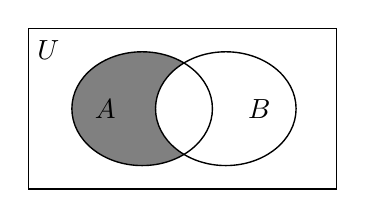
\begin{tikzpicture}[scale=0.85,line width=0.5pt]
\draw (0,0) rectangle (4.6,2.4);
\fill[gray] (1.7,1.2) ellipse (1.05 and 0.85);
\fill[white] (2.95,1.2) ellipse (1.05 and 0.85);
\draw (1.7,1.2) ellipse (1.05 and 0.85);
\draw (2.95,1.2) ellipse (1.05 and 0.85);
\node at (1.15,1.2) {$A$};
\node at (3.45,1.2) {$B$};
\node at (0.3,2.08) {$U$};
\end{tikzpicture}
\end{center}

\ifanswer
\solbegin
\step{$A=\{x\mid y=\sqrt{-x^2+x+2}\}=\{x\mid-1\leqslant x\leqslant2\}$，}
\step{$\overline B=\{x\mid 0\leqslant x\leqslant5\}$，$C=A\cap\overline B=[0,2]$.}
\solend
\fi

\item 关于 $x$ 的不等式 $ax-b<0$ 的解集为 $(2,+\infty)$，则关于 $x$ 的不等式 $(ax+b)(x-1)<0$ 的解集为\blankline[4.4em].

\ifanswer
\solbegin
\step{因为关于 $x$ 的不等式 $ax-b<0$ 的解集为 $(2,+\infty)$，所以 $\begin{cases}a<0\\2a-b=0\end{cases}$，}
\step{所以不等式 $(ax+b)(x-1)<0$ 可化为 $a\left(x+\dfrac ba\right)(x-1)<0$，$a<0$，}
\step{所以 $(x+2)(x-1)>0$，}
\step{所以所求解集为 $(-\infty,-2)\cup(1,+\infty)$.}
\solend
\fi

\item $a_1$、$b_1$、$a_2$、$b_2$ 均为非零实数，不等式 $a_1x+b_1>0$ 和 $a_2x+b_2>0$ 的解集分别为集合 $M$、$N$，那么“$\dfrac{a_1}{a_2}=\dfrac{b_1}{b_2}$”是“$M=N$”的\blankline[4.4em]条件（选填“充分非必要”、“必要非充分”、“充要”和“既非充分也非必要”）.

\ifanswer
\solbegin
\step{当 $a_1=b_1=1$，$a_2=b_2=-1$ 时，满足 $\dfrac{a_1}{a_2}=\dfrac{b_1}{b_2}$，}
\step{但是 $M=N$ 不成立，即充分性不成立；}
\step{若 $M=N$ 时，$\dfrac{a_1}{a_2}=\dfrac{b_1}{b_2}$ 一定成立，即必要性成立.}
\step{故为必要不充分条件.}% 原卷选项列“必要非充分”、解析结论作“必要不充分”，照录
\solend
\fi

\item 已知集合 $\{a,b,c\}=\{0,1,2\}$，且下列三个关系：① $a\neq2$；② $b=2$；③ $c\neq0$；有且只有一个正确，则 $100a+10b+c=$\blankline[4.4em].

\ifanswer
\solbegin
\step{列表如下：}
\begin{center}
\begin{tabular}{|c|c|c|c|c|}
\hline
 & ① & ② & ③ & \\
\hline
① 正确 & $a\neq2$ & $b\neq2$ & $c=0$ & 无解\\
\hline
② 正确 & $a=2$ & $b=2$ & $c=0$ & 矛盾\\
\hline
③ 正确 & $a=2$ & $b\neq2$ & $c\neq0$ & $a=2,b=0,c=1$\\
\hline
\end{tabular}
\end{center}
\step{所以 $100a+10b+c=201$.}
\solend
\fi

\end{enumerate}

\bigsec{二、选择题}

\begin{enumerate}
\setcounter{enumi}{12}

\item 已知 $a$,$b$,$c\in\R$,$b>c$，则下列不等式中恒成立的是\mbox{（\quad）}

\keepwithprev
A. $a+b^2>a+c^2$\qquad\quad B. $a^2+b>a^2+c$\qquad\quad C. $ab^2>ac^2$\qquad\quad D. $a^2b>a^2c$

\ifanswer
\solbegin
\step{对于 $A$，取 $b=1,c=-1$，错误；对于 $B$，由不等式的同向可加性得正确；}
\step{对于 $C$，取 $a=1,b=1,c=-2$，错误；对于 $D$，取 $a=0$，错误；}
\step{故选 $B$.}
\solend
\fi

\item 给出命题：“如果 $n$ 是素数，那么 $n^2+2$ 不是素数”，甲同学判断该命题是假命题，他做出这个判断的反例可以是\mbox{（\quad）}% 原卷把答案“$B$”印在题干括号内、无【解析】

\keepwithprev
A. $n=2$\qquad\quad B. $n=3$\qquad\quad C. $n=4$\qquad\quad D. $n=5$

\ifanswer
\ans{$B$}
\fi

\item 设集合 $A=\left\{x\,\middle\vert\,x=\dfrac n2,n\in\Z\right\}$，$B=\left\{x\,\middle\vert\,x=n+\dfrac12,n\in\Z\right\}$，则下列图形能表示 $A$ 与 $B$ 关系的是\mbox{（\quad）}

\keepwithprev
\begin{center}
% 原卷四个文氏图选项按原图形状用 TikZ 重排。
\begin{tabular}{c@{\qquad\qquad}c}
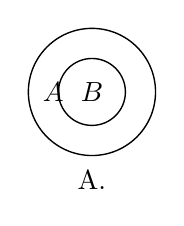
\begin{tikzpicture}[scale=0.85,line width=0.5pt]
\draw (0.9,0.9) circle (0.95);
\draw (0.9,0.9) circle (0.5);
\node at (0.32,0.9) {$A$};
\node at (0.9,0.9) {$B$};
\node[anchor=north] at (0.9,-0.12) {A.};
\end{tikzpicture}
&
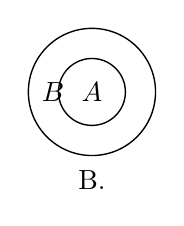
\begin{tikzpicture}[scale=0.85,line width=0.5pt]
\draw (0.9,0.9) circle (0.95);
\draw (0.9,0.9) circle (0.5);
\node at (0.32,0.9) {$B$};
\node at (0.9,0.9) {$A$};
\node[anchor=north] at (0.9,-0.12) {B.};
\end{tikzpicture}
\\[12pt]
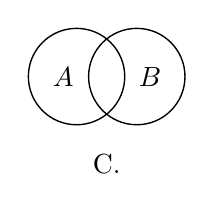
\begin{tikzpicture}[scale=0.85,line width=0.5pt]
\draw (0.65,0.9) circle (0.72);
\draw (1.55,0.9) circle (0.72);
\node at (0.45,0.9) {$A$};
\node at (1.75,0.9) {$B$};
\node[anchor=north] at (1.1,-0.12) {C.};
\end{tikzpicture}
&
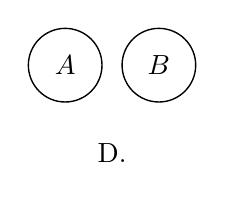
\begin{tikzpicture}[scale=0.85,line width=0.5pt]
\draw (0.55,0.9) circle (0.55);
\draw (1.95,0.9) circle (0.55);
\node at (0.55,0.9) {$A$};
\node at (1.95,0.9) {$B$};
\node[anchor=north] at (1.25,-0.12) {D.};
\end{tikzpicture}
\end{tabular}
\end{center}

\ifanswer
\solbegin
\step{$B\subset A$，图形能表示 $A$ 与 $B$ 关系的是 $A$. 故选 $A$.}
\solend
\fi

\item 以某些整数为元素的集合 $P$ 具有以下性质：

（1）$P$ 中元素有正数，也有负数；（2）$P$ 中元素有奇数，也有偶数；

（3）$-1\notin P$；（4）若 $x$、$y\in P$，则 $x+y\in P$.

则下列选项哪个是正确的\mbox{（\quad）}

\keepwithprev
A. 集合 $P$ 中一定有 $0$ 但没有 $2$\qquad\qquad B. 集合 $P$ 中一定有 $0$ 可能有 $2$

C. 集合 $P$ 中可能有 $0$ 可能有 $2$\qquad\qquad D. 集合 $P$ 中既没有 $0$ 又没有 $2$

\ifanswer
\solbegin
\step{由（4）得 $x\in P$，则 $kx\in P(k$ 是正整数$)$.}
\step{由（1）可设 $x$、$y\in P$，且 $x>0$，$y<0$，则 $xy$、$(-y)x\in P$，}
\step{因而 $0=xy+(-y)x\in P$.}
\step{假设 $2\in P$，则 $2k\in P$. 由上面及（4）得 $0$，$2$，$4$，$6$，$8$，$\cdots$ 均在 $P$ 中，}
\step{故 $2k-2\in P(k$ 是正整数$)$，}
\step{不妨令 $P$ 中负数为奇数 $-2k+1(k$ 为正整数$)$，}
\step{由（4）得 $(2k-2)+(-2k+1)=-1\in P$，矛盾.}
\step{故若 $2\in P$，则 $P$ 中没有负奇数.}
\step{若 $P$ 中负数为偶数，设为 $-2k(k$ 为正整数$)$，则由（4）及 $2\in P$，}
\step{得 $-2$,$-4$,$-6$,$\cdots$ 均在 $P$ 中，即 $-2m-2\in P(m$ 为非负整数$)$，}
\step{则 $P$ 中正奇数为 $2m+1$，由（4）得 $(-2m-2)+(2m+1)=-1\in P$，矛盾.}
\step{综上，$0\in P$，$2\notin P$，故选 $A$.}
\solend
\fi

\end{enumerate}

\bigsec{三、解答题}

\begin{enumerate}
\setcounter{enumi}{16}

\item （1）已知 $a$、$b$ 为实数，比较 $a^2+b^2$ 与 $4a-2b-5$ 的值的大小.

（2）若 $-1\leqslant x+y\leqslant2$，$-2\leqslant x-y\leqslant1$，求 $x-2y$ 的范围.

\ifanswer
\solbegin
\step{（1）$a^2+b^2-(4a-2b-5)=a^2-4a+4+b^2+2b+1=(a-2)^2+(b+1)^2\geqslant0$，}
\step{故 $a^2+b^2\geqslant4a-2b-5$.}
\step{（2）设 $x-2y=m(x+y)+n(x-y)$，则 $x-2y=(m+n)x+(m-n)y$，}
\step{所以 $\begin{cases}m+n=1\\m-n=-2\end{cases}$，解得 $n=\dfrac32$，$m=-\dfrac12$，}
\step{所以 $x-2y=-\dfrac12(x+y)+\dfrac32(x-y)$，}
\step{因为 $-1\leqslant x+y\leqslant2$，$-2\leqslant x-y\leqslant1$，}
\step{所以 $-1\leqslant-\dfrac12(x+y)\leqslant\dfrac12$，$-3\leqslant\dfrac32(x-y)\leqslant\dfrac32$，}
\step{所以 $-4\leqslant-\dfrac12(x+y)+\dfrac32(x-y)\leqslant2$，即 $-4\leqslant x-2y\leqslant2$，}
\step{故 $x-2y$ 的范围是 $[-4,2]$.}
\solend
\fi

\item 已知集合 $A=\{x\mid\lvert x-2\rvert<a\}$，集合 $B=\left\{x\,\middle\vert\,\dfrac{2x-1}{x+2}<1\right\}$.

（1）若 $a=2$，求 $A\cup B$,$A\cap B$；

（2）若 $A\cap B=A$，求实数 $a$ 的取值范围.

\ifanswer
\solbegin
\step{（1）由题意得 $A=(0,4)$,$B=(-2,3)$，所以 $A\cup B=(-2,4)$,$A\cap B=(0,3)$；}
\step{（2）因为 $A\cap B=A$，所以 $A\subseteq B$，}
\step{当 $a\leqslant0$ 时，$A=\varnothing$，满足 $A\subseteq B$；}
\step{当 $a>0$ 时，$A=(2-a,2+a)$,$B=(-2,3)$，}
\step{因为 $A\subseteq B$，所以 $\begin{cases}-2\leqslant2-a\\3\geqslant2+a\end{cases}$，解得 $a\leqslant1$，即 $0<a\leqslant1$.}
\step{因此，实数 $a$ 的取值范围为 $(-\infty,1]$.}
\solend
\fi

\item 我校校园文化节即将到来，高一年级将开展“数字配对”的抽奖活动，活动规则如下：每人可以抽取一张卡片，每张卡片上都印有一个不小于 $-10$ 且不大于 $10$ 的整数，其中不含 $2$. 每张卡片数字对应一个抽奖号码，卡片上的数字减去 $2$ 所得的差，与抽奖号码减去 $3$ 所得的差，两者的乘积等于 $12$.

（1）记卡片上的数字为 $x$，卡片数字对应的抽奖号码为 $y$，请用含有卡片数字 $x$ 的式子来表示抽奖号码 $y$；

（2）当抽奖号码不小于 $3$ 且不大于 $7$ 时，抽奖者可以领取奖品. 请问抽到哪些数字的卡片可以领取奖品？请写出满足领取奖品的卡片数字所组成的集合.

\ifanswer
\solbegin
\step{（1）卡片上的数字为 $x$，对应的抽奖号码为 $y$，}
\step{由题意得 $(x-2)(y-3)=12$，因为 $x\neq2$，所以 $y=3+\dfrac{12}{x-2}$，}
\step{所以 $y=3+\dfrac{12}{x-2}(-10\leqslant x\leqslant10,x\in\Z,x\neq2)$.}
\step{（2）由（1）得 $y=3+\dfrac{12}{x-2}(-10\leqslant x\leqslant10,x\in\Z,x\neq2)$，}
\step{由抽奖条件，得 $3\leqslant3+\dfrac{12}{x-2}\leqslant7$，$x\geqslant5$，所以 $5\leqslant x\leqslant10$，$x\in\Z$，}
\step{所以可领取奖品的卡片数字为 $\{5,6,7,8,9,10\}$.}
\solend
\fi

\item （1）已知 $m\in\R$，若不等式 $(m+1)x^2-mx+m-1<0$ 的解集是空集，求 $m$ 的取值范围；

（2）命题 $P:x^2-5x+6<0$，命题 $q:x^2-4ax+3a^2<0$，若命题 $P$ 是命题 $q$ 的充分非必要条件，求实数 $a$ 的取值范围.

\ifanswer
\solbegin
\step{（1）①当 $m+1=0$，即 $m=-1$ 时，$f(x)=x-2$，不合题意；}
\step{②当 $m+1\neq0$，即 $m\neq-1$ 时，$\begin{cases}m+1>0\\\Delta=m^2-4(m+1)(m-1)\leqslant0\end{cases}$，解得 $m\geqslant\dfrac{2\sqrt3}{3}$，}
\step{所以 $m$ 的取值范围是 $\left[\dfrac{2\sqrt3}{3},+\infty\right)$；}
\step{（2）解 $x^2-5x+6<0$，因式分解得 $(x-2)(x-3)<0$，故 $P$ 的解集为 $(2,3)$，}
\step{解 $x^2-4ax+3a^2<0$，因式分解得 $(x-a)(x-3a)<0$，}
\step{因为命题 $P$ 是命题 $q$ 的充分不必要条件，所以 $(2,3)$ 是 $q$ 解集的真子集，}
\step{当 $a=0$ 时，$q$ 的解集为 $\varnothing$，不合题意，舍去；}
\step{当 $a<0$ 时，$q$ 的解集为 $(3a,a)$，$\begin{cases}3a\leqslant2\\a\geqslant3\end{cases}$，不等式组无解，舍去；}
\step{当 $a>0$ 时，$q$ 的解集为 $(a,3a)$，又因为 $(2,3)$ 是 $q$ 解集的真子集，}
\step{所以 $\begin{cases}a\leqslant2\\3a\geqslant3\end{cases}$（等号不同时取），解得 $1\leqslant a\leqslant2$；}
\step{综上，实数 $a$ 的取值范围是 $[1,2]$.}
\solend
\fi

\item 对于至少含两个元素的有限正整数集 $A$，定义它的“两两和集”为
$S(A)=\{z\mid z=x+y$，其中 $x$、$y\in A$，且 $x<y\}$.

（1）若 $A=\{1,2,4,5\}$，求 $S(A)$；

（2）已知集合 $A$ 中恰好含有四个元素，且 $S(A)=\{5,7,8,10,11,13\}$，写出所有符合条件的集合 $A$；

（3）猜想：当集合 $A$ 含有 $n$ 个元素（$n\geqslant2$）时，$S(A)$ 的元素个数最少是多少？证明你的猜想.

\ifanswer
\solbegin
\step{（1）因为 $A=\{1,2,4,5\}$，计算所有两两和并去掉重复的结果有 $3$，$5$，$6$，$7$，$9$，}
\step{所以 $S(A)=\{3,5,6,7,9\}$.}
\step{（2）设 $A=\{a,b,c,d\}$，其中 $a<b<c<d$，且 $S(A)=\{5,7,8,10,11,13\}$，}
\step{四个元素共有六种两两配对，和集恰好有六个元素，}
\step{因此六个和互不相同.}
\step{这六个数分别为 $a+b$,$a+c$,$a+d$,$b+c$,$b+d$,$c+d$，}
\step{所以这六个数从小到大，可以确定第一个数为 $a+b$，第二数为 $a+c$，}
\step{第五个数为 $b+d$，第六数为 $c+d$，}
\step{第三个数和第四个数不能确定，即 $b+c$ 和 $a+d$ 的大小不定.}
\step{所以 $a+b=5$,$a+c=7$,$b+d=11$,$c+d=13$.}
\step{由此得到 $b=5-a$,$c=7-a$,$d=6+a$，}
\step{于是 $a+d=2a+6$,$b+c=12-2a$.}
\step{其余两个数 $b+c$,$a+d$ 对应 $8$,$10$，分两种情况讨论：}
\step{①若 $b+c=8$,$a+d=10$，则 $\begin{cases}12-2a=8\\2a+6=10\end{cases}$，解得 $a=2$，}
\step{所以 $A=\{2,3,5,8\}$；}
\step{②若 $b+c=10$,$a+d=8$，则 $\begin{cases}12-2a=10\\2a+6=8\end{cases}$，解得 $a=1$，}
\step{所以 $A=\{1,4,6,7\}$；}
\step{检验得，两组均符合题意.}
\step{因此所有符合条件的集合为 $A=\{1,4,6,7\}$ 或 $A=\{2,3,5,8\}$.}
\step{（3）猜想：两两和集的元素个数的最小值为 $2n-3$. 证明如下：}
\step{将集合中的元素按从小到大排列为 $a_1<a_2<\cdots<a_n$，}
\step{当 $n=2$ 时，两两和集恰好有一个元素，结论成立.}
\step{当 $n\geqslant3$ 时，考虑下列均属于 $S(A)$ 的数，}
\step{由不等式的传递性得严格不等式：}
\step{$a_1+a_2<a_1+a_3<\cdots<a_1+a_n<a_2+a_n<\cdots<a_{n-1}+a_n$，}
\step{其中 $a_1+a_2<a_1+a_3<\cdots<a_1+a_n$ 共有 $n-1$ 个不相等的数；}
\step{$a_2+a_n<\cdots<a_{n-1}+a_n$ 共有 $n-2$ 个不相等的数，}
\step{所以一共有 $(n-1)+(n-2)=2n-3$ 个，}
\step{因此，两两和集至少含有 $2n-3$ 个元素.}
\step{再证明可以取到 $2n-3$：}
\step{对任意 $n\geqslant2$，取 $A=\{1,2,\cdots,n\}$，}
\step{所有两两和都是不小于 $3$ 且不大于 $2n-1$ 的整数，}
\step{其中，$1+2$,$1+3$,$\cdots$,$1+n$ 是从 $3$ 到 $n+1$ 的整数；}
\step{当 $n\geqslant3$ 时，$2+n$,$3+n$,$\cdots$,$(n-1)+n$ 可取到其余整数；}
\step{因此 $S(A)=\{3,4,\cdots,2n-1\}$，其元素个数为 $(2n-1)-3+1=2n-3$，}
\step{所以所求最小值为 $2n-3$.}
\solend
\fi

\end{enumerate}

\end{document}
"
% 紧凑版：xelatex "\def\iscompact{1}% 高一118_罗店中学_10月月考.tex
%   —— 高一上数学“2026-2027 年罗店中学高一上 10 月月考”（试卷版/答案版）
% 试卷版：xelatex 高一118_罗店中学_10月月考.tex
% 答案版：xelatex "\def\isanswer{1}% 高一118_罗店中学_10月月考.tex
%   —— 高一上数学“2026-2027 年罗店中学高一上 10 月月考”（试卷版/答案版）
% 试卷版：xelatex 高一118_罗店中学_10月月考.tex
% 答案版：xelatex "\def\isanswer{1}\input{高一118_罗店中学_10月月考.tex}"
% 紧凑版：xelatex "\def\iscompact{1}\input{高一118_罗店中学_10月月考.tex}"
%
% 原始材料：微信公众号“魔都数学加油站”文章，作者破晓，2026-11-06 17:58 发布；
% 连载“27学年高一118”，原文标题“27学年高一118——2026-2027年上海市罗店中学高一上10月月考”；
% 原文链接：https://mp.weixin.qq.com/s/4edo8awYdjmWJl153X-aDA。
% 正文为 9 张 PNG 页（第 2、3、5、9 页 2560×3620，其余 4762×6735），
% 题目下印有【解析】或【答案】，为讲评版。
% 题目、解析均据原图转录；卷面红色水印及公众号页脚未录入。
%
% 卷首标题：原卷印作“2026-2027 年罗店中学高一上 10 月月考”（公众号标题中的“上海市”
% 卷面标题行没有，本稿照卷面），年份区间按全稿惯例排 en dash；原卷未印副标题，本稿按题目内容
% 标为“集合与常用逻辑用语、不等式”。
%
% 与原卷的排版差异：
%   ① 原文从第 3 题起，填空题 3—12、选择题 13—16、解答题 17—21，共 19 题，本稿保留原题号；
%   ② 原卷每题下直接印【解析】／【答案】，本稿按全稿惯例置于答案版；第 4 题只印【答案】、
%      第 14 题把答案“$B$”印在题干括号内且无【解析】，均另提 \ans{}；其余选择题答案在
%      解析末句“故选 …”，括号内留空；
%   ③ 原卷未印副标题，本稿按“知识模块”口径补出；
%   ④ 原卷填空横线按全稿惯例排为 \blankline[4.4em]；选择题括号排 \mbox{（\quad）}、
%      选项段前按惯例加 \keepwithprev；解答题不留作答区（原卷为讲评版，与 109—117 同）；
%   ⑤ 原卷数集 $R$／$Z$ 按全稿惯例改 \R、\Z，补集照原卷上划线排 \overline{B}。
%
% 子集符号：第 6 题、第 18 题的 $\{x\mid x<1\}\subseteq\{x\mid x<3a-2\}$ 与 $A\subseteq B$
%   印有下划线，照录 \subseteq；第 15 题解析的 $B\subset A$ 印单线（真子集、无下划线），
%   按 18／96 成例照录 \subset。
%
% 判别式字形：第 20 题 (1) cases 的判别式原卷排 $\Delta$（等腰、右厚），照录 \Delta。
%
% 图与表：第 9 题题干的文氏图（矩形 $U$ 内两椭圆 $A$、$B$，阴影为 $A\cap\overline B$）
%   按原图形状用 TikZ 重绘（三版都出）；第 12 题解析的“列表”按原卷用 tabular 重排
%   （仅答案版）；第 15 题四个文氏图选项按原图形状用 TikZ 重排（三版都出）。
%
% 原卷存疑照录：第 8 题解析“$2022+3\cdot1\cdot(-1)=2026$”一行、第 11 题解析结论
%   作“必要不充分条件”而选项列“必要非充分”、第 20 题 (2) 的 cases，均照录加注。
%
% 行数核对：逐题数 \step/\stepm 条数，合计 110 条（Q3：2；Q4：0；Q5：1；Q6：2；Q7：5；
% Q8：3；Q9：2；Q10：4；Q11：4；Q12：2；Q13：3；Q14：0；Q15：1；Q16：12；Q17：9；
% Q18：6；Q19：6；Q20：11；Q21：36），与原卷印刷行逐题相等（cases／tabular／TikZ
% 图块作一个印刷行计）。第 4 题只印【答案】、第 14 题括号内印答案且无解析，均提 \ans{}，
% 不计入 \step 账。
%
\documentclass[a4paper,11pt]{article}
\usepackage{common}

\begin{document}

\examtitlest[3]{2026--2027 年罗店中学高一上 10 月月考}{集合与常用逻辑用语、不等式}

\bigsec{一、填空题}

\begin{enumerate}
\setcounter{enumi}{2}

\item 若 $2x^2+3x+5=a(2x+1)(x+1)+b$ 恒成立，则 $a-b$ 的值\blankline[4.4em].

\ifanswer
\solbegin
\step{因为 $2x^2+3x+5=a(2x+1)(x+1)+b=2ax^2+3ax+a+b$ 恒成立，}
\step{所以 $\begin{cases}2=2a\\3=3a\\5=a+b\end{cases}$，所以 $\begin{cases}a=1\\b=4\end{cases}$，故 $a-b$ 的值为 $-3$.}
\solend
\fi

\item “$a$、$b$ 中至少有一个能被 $6$ 整除”的否定形式是\blankline[4.4em].

\ifanswer
\ans{$a$、$b$ 都不能被 $6$ 整除}
\fi

\item 设集合 $A=\{1,2\}$，则满足 $A\cup B=\{1,2,3\}$ 的集合 $B$ 的个数是\blankline[4.4em].

\ifanswer
\solbegin
\step{$B=\{3\}$,$\{1,3\}$,$\{2,3\}$,$\{1,2,3\}$，个数为 $4$.}
\solend
\fi

\item 命题“若 $x<1$，则 $x<3a-2$”是真命题，求实数 $a$ 的取值范围是\blankline[4.4em].

\ifanswer
\solbegin
\step{$\alpha:x<1$,$\beta:x<3a-2$，且若 $\alpha$ 则 $\beta$ 是真命题，}
\step{则 $\{x\mid x<1\}\subseteq\{x\mid x<3a-2\}$，所以 $3a-2\geqslant1$，解得 $a\geqslant1$.}
\solend
\fi

\item 不论实数 $m$ 取什么值，点 $P(m+1,2-m)$ 一定不在第\blankline[4.4em]象限（选填“一”、“二”、“三”或“四”）.

\ifanswer
\solbegin
\step{当 $m+1>0$，$2-m>0$ 时，解得 $-1<m<2$，此时点 $P$ 在第一象限；}
\step{当 $m+1<0$，$2-m>0$ 时，解得 $m<-1$，此时点 $P$ 在第二象限；}
\step{当 $m+1<0$，$2-m<0$ 时，$m$ 无解，此时点 $P$ 不可能在第三象限；}
\step{当 $m+1>0$，$2-m<0$ 时，解得 $m>2$，此时点 $P$ 在第四象限.}
\step{故一定不在第三象限.}
\solend
\fi

\item 设 $x_1$、$x_2$ 是方程 $x^2+x-3=0$ 的两个实数根，则 $x_1^2-x_2+2022=$\blankline[4.4em].

\ifanswer
\solbegin
\step{$x_1$、$x_2$ 是方程 $x^2+x-3=0$ 的两个实数根，}
\step{得 $x_1+x_2=-1$，$x_1^2+x_1-3=0$，所以 $x_1^2=3-x_1$，}
\step{$x_1^2-x_2+2022=3-x_1-x_2+2022=2022+3\cdot1\cdot(-1)=2026$.}
\solend
\fi

\item 如图，已知全集 $U=\R$，集合 $A=\{x\mid y=\sqrt{-x^2+x+2}\}$，$B=\{x\mid x<0$ 或 $x>5\}$. 集合 $C$ 表示图中阴影区域对应的集合，则集合 $C=$\blankline[4.4em]（用区间表示）.

\begin{center}
% 原卷文氏图：矩形 U 内两椭圆 A（阴影）、B，阴影为 A\cap\overline B，按原图形状用 TikZ 重绘。
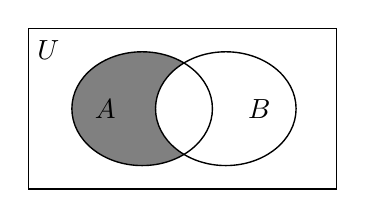
\begin{tikzpicture}[scale=0.85,line width=0.5pt]
\draw (0,0) rectangle (4.6,2.4);
\fill[gray] (1.7,1.2) ellipse (1.05 and 0.85);
\fill[white] (2.95,1.2) ellipse (1.05 and 0.85);
\draw (1.7,1.2) ellipse (1.05 and 0.85);
\draw (2.95,1.2) ellipse (1.05 and 0.85);
\node at (1.15,1.2) {$A$};
\node at (3.45,1.2) {$B$};
\node at (0.3,2.08) {$U$};
\end{tikzpicture}
\end{center}

\ifanswer
\solbegin
\step{$A=\{x\mid y=\sqrt{-x^2+x+2}\}=\{x\mid-1\leqslant x\leqslant2\}$，}
\step{$\overline B=\{x\mid 0\leqslant x\leqslant5\}$，$C=A\cap\overline B=[0,2]$.}
\solend
\fi

\item 关于 $x$ 的不等式 $ax-b<0$ 的解集为 $(2,+\infty)$，则关于 $x$ 的不等式 $(ax+b)(x-1)<0$ 的解集为\blankline[4.4em].

\ifanswer
\solbegin
\step{因为关于 $x$ 的不等式 $ax-b<0$ 的解集为 $(2,+\infty)$，所以 $\begin{cases}a<0\\2a-b=0\end{cases}$，}
\step{所以不等式 $(ax+b)(x-1)<0$ 可化为 $a\left(x+\dfrac ba\right)(x-1)<0$，$a<0$，}
\step{所以 $(x+2)(x-1)>0$，}
\step{所以所求解集为 $(-\infty,-2)\cup(1,+\infty)$.}
\solend
\fi

\item $a_1$、$b_1$、$a_2$、$b_2$ 均为非零实数，不等式 $a_1x+b_1>0$ 和 $a_2x+b_2>0$ 的解集分别为集合 $M$、$N$，那么“$\dfrac{a_1}{a_2}=\dfrac{b_1}{b_2}$”是“$M=N$”的\blankline[4.4em]条件（选填“充分非必要”、“必要非充分”、“充要”和“既非充分也非必要”）.

\ifanswer
\solbegin
\step{当 $a_1=b_1=1$，$a_2=b_2=-1$ 时，满足 $\dfrac{a_1}{a_2}=\dfrac{b_1}{b_2}$，}
\step{但是 $M=N$ 不成立，即充分性不成立；}
\step{若 $M=N$ 时，$\dfrac{a_1}{a_2}=\dfrac{b_1}{b_2}$ 一定成立，即必要性成立.}
\step{故为必要不充分条件.}% 原卷选项列“必要非充分”、解析结论作“必要不充分”，照录
\solend
\fi

\item 已知集合 $\{a,b,c\}=\{0,1,2\}$，且下列三个关系：① $a\neq2$；② $b=2$；③ $c\neq0$；有且只有一个正确，则 $100a+10b+c=$\blankline[4.4em].

\ifanswer
\solbegin
\step{列表如下：}
\begin{center}
\begin{tabular}{|c|c|c|c|c|}
\hline
 & ① & ② & ③ & \\
\hline
① 正确 & $a\neq2$ & $b\neq2$ & $c=0$ & 无解\\
\hline
② 正确 & $a=2$ & $b=2$ & $c=0$ & 矛盾\\
\hline
③ 正确 & $a=2$ & $b\neq2$ & $c\neq0$ & $a=2,b=0,c=1$\\
\hline
\end{tabular}
\end{center}
\step{所以 $100a+10b+c=201$.}
\solend
\fi

\end{enumerate}

\bigsec{二、选择题}

\begin{enumerate}
\setcounter{enumi}{12}

\item 已知 $a$,$b$,$c\in\R$,$b>c$，则下列不等式中恒成立的是\mbox{（\quad）}

\keepwithprev
A. $a+b^2>a+c^2$\qquad\quad B. $a^2+b>a^2+c$\qquad\quad C. $ab^2>ac^2$\qquad\quad D. $a^2b>a^2c$

\ifanswer
\solbegin
\step{对于 $A$，取 $b=1,c=-1$，错误；对于 $B$，由不等式的同向可加性得正确；}
\step{对于 $C$，取 $a=1,b=1,c=-2$，错误；对于 $D$，取 $a=0$，错误；}
\step{故选 $B$.}
\solend
\fi

\item 给出命题：“如果 $n$ 是素数，那么 $n^2+2$ 不是素数”，甲同学判断该命题是假命题，他做出这个判断的反例可以是\mbox{（\quad）}% 原卷把答案“$B$”印在题干括号内、无【解析】

\keepwithprev
A. $n=2$\qquad\quad B. $n=3$\qquad\quad C. $n=4$\qquad\quad D. $n=5$

\ifanswer
\ans{$B$}
\fi

\item 设集合 $A=\left\{x\,\middle\vert\,x=\dfrac n2,n\in\Z\right\}$，$B=\left\{x\,\middle\vert\,x=n+\dfrac12,n\in\Z\right\}$，则下列图形能表示 $A$ 与 $B$ 关系的是\mbox{（\quad）}

\keepwithprev
\begin{center}
% 原卷四个文氏图选项按原图形状用 TikZ 重排。
\begin{tabular}{c@{\qquad\qquad}c}
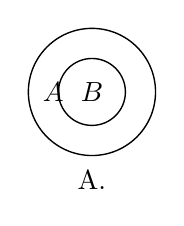
\begin{tikzpicture}[scale=0.85,line width=0.5pt]
\draw (0.9,0.9) circle (0.95);
\draw (0.9,0.9) circle (0.5);
\node at (0.32,0.9) {$A$};
\node at (0.9,0.9) {$B$};
\node[anchor=north] at (0.9,-0.12) {A.};
\end{tikzpicture}
&
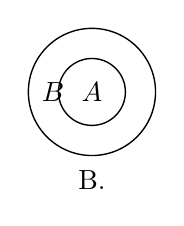
\begin{tikzpicture}[scale=0.85,line width=0.5pt]
\draw (0.9,0.9) circle (0.95);
\draw (0.9,0.9) circle (0.5);
\node at (0.32,0.9) {$B$};
\node at (0.9,0.9) {$A$};
\node[anchor=north] at (0.9,-0.12) {B.};
\end{tikzpicture}
\\[12pt]
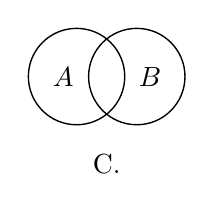
\begin{tikzpicture}[scale=0.85,line width=0.5pt]
\draw (0.65,0.9) circle (0.72);
\draw (1.55,0.9) circle (0.72);
\node at (0.45,0.9) {$A$};
\node at (1.75,0.9) {$B$};
\node[anchor=north] at (1.1,-0.12) {C.};
\end{tikzpicture}
&
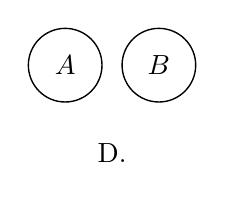
\begin{tikzpicture}[scale=0.85,line width=0.5pt]
\draw (0.55,0.9) circle (0.55);
\draw (1.95,0.9) circle (0.55);
\node at (0.55,0.9) {$A$};
\node at (1.95,0.9) {$B$};
\node[anchor=north] at (1.25,-0.12) {D.};
\end{tikzpicture}
\end{tabular}
\end{center}

\ifanswer
\solbegin
\step{$B\subset A$，图形能表示 $A$ 与 $B$ 关系的是 $A$. 故选 $A$.}
\solend
\fi

\item 以某些整数为元素的集合 $P$ 具有以下性质：

（1）$P$ 中元素有正数，也有负数；（2）$P$ 中元素有奇数，也有偶数；

（3）$-1\notin P$；（4）若 $x$、$y\in P$，则 $x+y\in P$.

则下列选项哪个是正确的\mbox{（\quad）}

\keepwithprev
A. 集合 $P$ 中一定有 $0$ 但没有 $2$\qquad\qquad B. 集合 $P$ 中一定有 $0$ 可能有 $2$

C. 集合 $P$ 中可能有 $0$ 可能有 $2$\qquad\qquad D. 集合 $P$ 中既没有 $0$ 又没有 $2$

\ifanswer
\solbegin
\step{由（4）得 $x\in P$，则 $kx\in P(k$ 是正整数$)$.}
\step{由（1）可设 $x$、$y\in P$，且 $x>0$，$y<0$，则 $xy$、$(-y)x\in P$，}
\step{因而 $0=xy+(-y)x\in P$.}
\step{假设 $2\in P$，则 $2k\in P$. 由上面及（4）得 $0$，$2$，$4$，$6$，$8$，$\cdots$ 均在 $P$ 中，}
\step{故 $2k-2\in P(k$ 是正整数$)$，}
\step{不妨令 $P$ 中负数为奇数 $-2k+1(k$ 为正整数$)$，}
\step{由（4）得 $(2k-2)+(-2k+1)=-1\in P$，矛盾.}
\step{故若 $2\in P$，则 $P$ 中没有负奇数.}
\step{若 $P$ 中负数为偶数，设为 $-2k(k$ 为正整数$)$，则由（4）及 $2\in P$，}
\step{得 $-2$,$-4$,$-6$,$\cdots$ 均在 $P$ 中，即 $-2m-2\in P(m$ 为非负整数$)$，}
\step{则 $P$ 中正奇数为 $2m+1$，由（4）得 $(-2m-2)+(2m+1)=-1\in P$，矛盾.}
\step{综上，$0\in P$，$2\notin P$，故选 $A$.}
\solend
\fi

\end{enumerate}

\bigsec{三、解答题}

\begin{enumerate}
\setcounter{enumi}{16}

\item （1）已知 $a$、$b$ 为实数，比较 $a^2+b^2$ 与 $4a-2b-5$ 的值的大小.

（2）若 $-1\leqslant x+y\leqslant2$，$-2\leqslant x-y\leqslant1$，求 $x-2y$ 的范围.

\ifanswer
\solbegin
\step{（1）$a^2+b^2-(4a-2b-5)=a^2-4a+4+b^2+2b+1=(a-2)^2+(b+1)^2\geqslant0$，}
\step{故 $a^2+b^2\geqslant4a-2b-5$.}
\step{（2）设 $x-2y=m(x+y)+n(x-y)$，则 $x-2y=(m+n)x+(m-n)y$，}
\step{所以 $\begin{cases}m+n=1\\m-n=-2\end{cases}$，解得 $n=\dfrac32$，$m=-\dfrac12$，}
\step{所以 $x-2y=-\dfrac12(x+y)+\dfrac32(x-y)$，}
\step{因为 $-1\leqslant x+y\leqslant2$，$-2\leqslant x-y\leqslant1$，}
\step{所以 $-1\leqslant-\dfrac12(x+y)\leqslant\dfrac12$，$-3\leqslant\dfrac32(x-y)\leqslant\dfrac32$，}
\step{所以 $-4\leqslant-\dfrac12(x+y)+\dfrac32(x-y)\leqslant2$，即 $-4\leqslant x-2y\leqslant2$，}
\step{故 $x-2y$ 的范围是 $[-4,2]$.}
\solend
\fi

\item 已知集合 $A=\{x\mid\lvert x-2\rvert<a\}$，集合 $B=\left\{x\,\middle\vert\,\dfrac{2x-1}{x+2}<1\right\}$.

（1）若 $a=2$，求 $A\cup B$,$A\cap B$；

（2）若 $A\cap B=A$，求实数 $a$ 的取值范围.

\ifanswer
\solbegin
\step{（1）由题意得 $A=(0,4)$,$B=(-2,3)$，所以 $A\cup B=(-2,4)$,$A\cap B=(0,3)$；}
\step{（2）因为 $A\cap B=A$，所以 $A\subseteq B$，}
\step{当 $a\leqslant0$ 时，$A=\varnothing$，满足 $A\subseteq B$；}
\step{当 $a>0$ 时，$A=(2-a,2+a)$,$B=(-2,3)$，}
\step{因为 $A\subseteq B$，所以 $\begin{cases}-2\leqslant2-a\\3\geqslant2+a\end{cases}$，解得 $a\leqslant1$，即 $0<a\leqslant1$.}
\step{因此，实数 $a$ 的取值范围为 $(-\infty,1]$.}
\solend
\fi

\item 我校校园文化节即将到来，高一年级将开展“数字配对”的抽奖活动，活动规则如下：每人可以抽取一张卡片，每张卡片上都印有一个不小于 $-10$ 且不大于 $10$ 的整数，其中不含 $2$. 每张卡片数字对应一个抽奖号码，卡片上的数字减去 $2$ 所得的差，与抽奖号码减去 $3$ 所得的差，两者的乘积等于 $12$.

（1）记卡片上的数字为 $x$，卡片数字对应的抽奖号码为 $y$，请用含有卡片数字 $x$ 的式子来表示抽奖号码 $y$；

（2）当抽奖号码不小于 $3$ 且不大于 $7$ 时，抽奖者可以领取奖品. 请问抽到哪些数字的卡片可以领取奖品？请写出满足领取奖品的卡片数字所组成的集合.

\ifanswer
\solbegin
\step{（1）卡片上的数字为 $x$，对应的抽奖号码为 $y$，}
\step{由题意得 $(x-2)(y-3)=12$，因为 $x\neq2$，所以 $y=3+\dfrac{12}{x-2}$，}
\step{所以 $y=3+\dfrac{12}{x-2}(-10\leqslant x\leqslant10,x\in\Z,x\neq2)$.}
\step{（2）由（1）得 $y=3+\dfrac{12}{x-2}(-10\leqslant x\leqslant10,x\in\Z,x\neq2)$，}
\step{由抽奖条件，得 $3\leqslant3+\dfrac{12}{x-2}\leqslant7$，$x\geqslant5$，所以 $5\leqslant x\leqslant10$，$x\in\Z$，}
\step{所以可领取奖品的卡片数字为 $\{5,6,7,8,9,10\}$.}
\solend
\fi

\item （1）已知 $m\in\R$，若不等式 $(m+1)x^2-mx+m-1<0$ 的解集是空集，求 $m$ 的取值范围；

（2）命题 $P:x^2-5x+6<0$，命题 $q:x^2-4ax+3a^2<0$，若命题 $P$ 是命题 $q$ 的充分非必要条件，求实数 $a$ 的取值范围.

\ifanswer
\solbegin
\step{（1）①当 $m+1=0$，即 $m=-1$ 时，$f(x)=x-2$，不合题意；}
\step{②当 $m+1\neq0$，即 $m\neq-1$ 时，$\begin{cases}m+1>0\\\Delta=m^2-4(m+1)(m-1)\leqslant0\end{cases}$，解得 $m\geqslant\dfrac{2\sqrt3}{3}$，}
\step{所以 $m$ 的取值范围是 $\left[\dfrac{2\sqrt3}{3},+\infty\right)$；}
\step{（2）解 $x^2-5x+6<0$，因式分解得 $(x-2)(x-3)<0$，故 $P$ 的解集为 $(2,3)$，}
\step{解 $x^2-4ax+3a^2<0$，因式分解得 $(x-a)(x-3a)<0$，}
\step{因为命题 $P$ 是命题 $q$ 的充分不必要条件，所以 $(2,3)$ 是 $q$ 解集的真子集，}
\step{当 $a=0$ 时，$q$ 的解集为 $\varnothing$，不合题意，舍去；}
\step{当 $a<0$ 时，$q$ 的解集为 $(3a,a)$，$\begin{cases}3a\leqslant2\\a\geqslant3\end{cases}$，不等式组无解，舍去；}
\step{当 $a>0$ 时，$q$ 的解集为 $(a,3a)$，又因为 $(2,3)$ 是 $q$ 解集的真子集，}
\step{所以 $\begin{cases}a\leqslant2\\3a\geqslant3\end{cases}$（等号不同时取），解得 $1\leqslant a\leqslant2$；}
\step{综上，实数 $a$ 的取值范围是 $[1,2]$.}
\solend
\fi

\item 对于至少含两个元素的有限正整数集 $A$，定义它的“两两和集”为
$S(A)=\{z\mid z=x+y$，其中 $x$、$y\in A$，且 $x<y\}$.

（1）若 $A=\{1,2,4,5\}$，求 $S(A)$；

（2）已知集合 $A$ 中恰好含有四个元素，且 $S(A)=\{5,7,8,10,11,13\}$，写出所有符合条件的集合 $A$；

（3）猜想：当集合 $A$ 含有 $n$ 个元素（$n\geqslant2$）时，$S(A)$ 的元素个数最少是多少？证明你的猜想.

\ifanswer
\solbegin
\step{（1）因为 $A=\{1,2,4,5\}$，计算所有两两和并去掉重复的结果有 $3$，$5$，$6$，$7$，$9$，}
\step{所以 $S(A)=\{3,5,6,7,9\}$.}
\step{（2）设 $A=\{a,b,c,d\}$，其中 $a<b<c<d$，且 $S(A)=\{5,7,8,10,11,13\}$，}
\step{四个元素共有六种两两配对，和集恰好有六个元素，}
\step{因此六个和互不相同.}
\step{这六个数分别为 $a+b$,$a+c$,$a+d$,$b+c$,$b+d$,$c+d$，}
\step{所以这六个数从小到大，可以确定第一个数为 $a+b$，第二数为 $a+c$，}
\step{第五个数为 $b+d$，第六数为 $c+d$，}
\step{第三个数和第四个数不能确定，即 $b+c$ 和 $a+d$ 的大小不定.}
\step{所以 $a+b=5$,$a+c=7$,$b+d=11$,$c+d=13$.}
\step{由此得到 $b=5-a$,$c=7-a$,$d=6+a$，}
\step{于是 $a+d=2a+6$,$b+c=12-2a$.}
\step{其余两个数 $b+c$,$a+d$ 对应 $8$,$10$，分两种情况讨论：}
\step{①若 $b+c=8$,$a+d=10$，则 $\begin{cases}12-2a=8\\2a+6=10\end{cases}$，解得 $a=2$，}
\step{所以 $A=\{2,3,5,8\}$；}
\step{②若 $b+c=10$,$a+d=8$，则 $\begin{cases}12-2a=10\\2a+6=8\end{cases}$，解得 $a=1$，}
\step{所以 $A=\{1,4,6,7\}$；}
\step{检验得，两组均符合题意.}
\step{因此所有符合条件的集合为 $A=\{1,4,6,7\}$ 或 $A=\{2,3,5,8\}$.}
\step{（3）猜想：两两和集的元素个数的最小值为 $2n-3$. 证明如下：}
\step{将集合中的元素按从小到大排列为 $a_1<a_2<\cdots<a_n$，}
\step{当 $n=2$ 时，两两和集恰好有一个元素，结论成立.}
\step{当 $n\geqslant3$ 时，考虑下列均属于 $S(A)$ 的数，}
\step{由不等式的传递性得严格不等式：}
\step{$a_1+a_2<a_1+a_3<\cdots<a_1+a_n<a_2+a_n<\cdots<a_{n-1}+a_n$，}
\step{其中 $a_1+a_2<a_1+a_3<\cdots<a_1+a_n$ 共有 $n-1$ 个不相等的数；}
\step{$a_2+a_n<\cdots<a_{n-1}+a_n$ 共有 $n-2$ 个不相等的数，}
\step{所以一共有 $(n-1)+(n-2)=2n-3$ 个，}
\step{因此，两两和集至少含有 $2n-3$ 个元素.}
\step{再证明可以取到 $2n-3$：}
\step{对任意 $n\geqslant2$，取 $A=\{1,2,\cdots,n\}$，}
\step{所有两两和都是不小于 $3$ 且不大于 $2n-1$ 的整数，}
\step{其中，$1+2$,$1+3$,$\cdots$,$1+n$ 是从 $3$ 到 $n+1$ 的整数；}
\step{当 $n\geqslant3$ 时，$2+n$,$3+n$,$\cdots$,$(n-1)+n$ 可取到其余整数；}
\step{因此 $S(A)=\{3,4,\cdots,2n-1\}$，其元素个数为 $(2n-1)-3+1=2n-3$，}
\step{所以所求最小值为 $2n-3$.}
\solend
\fi

\end{enumerate}

\end{document}
"
% 紧凑版：xelatex "\def\iscompact{1}% 高一118_罗店中学_10月月考.tex
%   —— 高一上数学“2026-2027 年罗店中学高一上 10 月月考”（试卷版/答案版）
% 试卷版：xelatex 高一118_罗店中学_10月月考.tex
% 答案版：xelatex "\def\isanswer{1}\input{高一118_罗店中学_10月月考.tex}"
% 紧凑版：xelatex "\def\iscompact{1}\input{高一118_罗店中学_10月月考.tex}"
%
% 原始材料：微信公众号“魔都数学加油站”文章，作者破晓，2026-11-06 17:58 发布；
% 连载“27学年高一118”，原文标题“27学年高一118——2026-2027年上海市罗店中学高一上10月月考”；
% 原文链接：https://mp.weixin.qq.com/s/4edo8awYdjmWJl153X-aDA。
% 正文为 9 张 PNG 页（第 2、3、5、9 页 2560×3620，其余 4762×6735），
% 题目下印有【解析】或【答案】，为讲评版。
% 题目、解析均据原图转录；卷面红色水印及公众号页脚未录入。
%
% 卷首标题：原卷印作“2026-2027 年罗店中学高一上 10 月月考”（公众号标题中的“上海市”
% 卷面标题行没有，本稿照卷面），年份区间按全稿惯例排 en dash；原卷未印副标题，本稿按题目内容
% 标为“集合与常用逻辑用语、不等式”。
%
% 与原卷的排版差异：
%   ① 原文从第 3 题起，填空题 3—12、选择题 13—16、解答题 17—21，共 19 题，本稿保留原题号；
%   ② 原卷每题下直接印【解析】／【答案】，本稿按全稿惯例置于答案版；第 4 题只印【答案】、
%      第 14 题把答案“$B$”印在题干括号内且无【解析】，均另提 \ans{}；其余选择题答案在
%      解析末句“故选 …”，括号内留空；
%   ③ 原卷未印副标题，本稿按“知识模块”口径补出；
%   ④ 原卷填空横线按全稿惯例排为 \blankline[4.4em]；选择题括号排 \mbox{（\quad）}、
%      选项段前按惯例加 \keepwithprev；解答题不留作答区（原卷为讲评版，与 109—117 同）；
%   ⑤ 原卷数集 $R$／$Z$ 按全稿惯例改 \R、\Z，补集照原卷上划线排 \overline{B}。
%
% 子集符号：第 6 题、第 18 题的 $\{x\mid x<1\}\subseteq\{x\mid x<3a-2\}$ 与 $A\subseteq B$
%   印有下划线，照录 \subseteq；第 15 题解析的 $B\subset A$ 印单线（真子集、无下划线），
%   按 18／96 成例照录 \subset。
%
% 判别式字形：第 20 题 (1) cases 的判别式原卷排 $\Delta$（等腰、右厚），照录 \Delta。
%
% 图与表：第 9 题题干的文氏图（矩形 $U$ 内两椭圆 $A$、$B$，阴影为 $A\cap\overline B$）
%   按原图形状用 TikZ 重绘（三版都出）；第 12 题解析的“列表”按原卷用 tabular 重排
%   （仅答案版）；第 15 题四个文氏图选项按原图形状用 TikZ 重排（三版都出）。
%
% 原卷存疑照录：第 8 题解析“$2022+3\cdot1\cdot(-1)=2026$”一行、第 11 题解析结论
%   作“必要不充分条件”而选项列“必要非充分”、第 20 题 (2) 的 cases，均照录加注。
%
% 行数核对：逐题数 \step/\stepm 条数，合计 110 条（Q3：2；Q4：0；Q5：1；Q6：2；Q7：5；
% Q8：3；Q9：2；Q10：4；Q11：4；Q12：2；Q13：3；Q14：0；Q15：1；Q16：12；Q17：9；
% Q18：6；Q19：6；Q20：11；Q21：36），与原卷印刷行逐题相等（cases／tabular／TikZ
% 图块作一个印刷行计）。第 4 题只印【答案】、第 14 题括号内印答案且无解析，均提 \ans{}，
% 不计入 \step 账。
%
\documentclass[a4paper,11pt]{article}
\usepackage{common}

\begin{document}

\examtitlest[3]{2026--2027 年罗店中学高一上 10 月月考}{集合与常用逻辑用语、不等式}

\bigsec{一、填空题}

\begin{enumerate}
\setcounter{enumi}{2}

\item 若 $2x^2+3x+5=a(2x+1)(x+1)+b$ 恒成立，则 $a-b$ 的值\blankline[4.4em].

\ifanswer
\solbegin
\step{因为 $2x^2+3x+5=a(2x+1)(x+1)+b=2ax^2+3ax+a+b$ 恒成立，}
\step{所以 $\begin{cases}2=2a\\3=3a\\5=a+b\end{cases}$，所以 $\begin{cases}a=1\\b=4\end{cases}$，故 $a-b$ 的值为 $-3$.}
\solend
\fi

\item “$a$、$b$ 中至少有一个能被 $6$ 整除”的否定形式是\blankline[4.4em].

\ifanswer
\ans{$a$、$b$ 都不能被 $6$ 整除}
\fi

\item 设集合 $A=\{1,2\}$，则满足 $A\cup B=\{1,2,3\}$ 的集合 $B$ 的个数是\blankline[4.4em].

\ifanswer
\solbegin
\step{$B=\{3\}$,$\{1,3\}$,$\{2,3\}$,$\{1,2,3\}$，个数为 $4$.}
\solend
\fi

\item 命题“若 $x<1$，则 $x<3a-2$”是真命题，求实数 $a$ 的取值范围是\blankline[4.4em].

\ifanswer
\solbegin
\step{$\alpha:x<1$,$\beta:x<3a-2$，且若 $\alpha$ 则 $\beta$ 是真命题，}
\step{则 $\{x\mid x<1\}\subseteq\{x\mid x<3a-2\}$，所以 $3a-2\geqslant1$，解得 $a\geqslant1$.}
\solend
\fi

\item 不论实数 $m$ 取什么值，点 $P(m+1,2-m)$ 一定不在第\blankline[4.4em]象限（选填“一”、“二”、“三”或“四”）.

\ifanswer
\solbegin
\step{当 $m+1>0$，$2-m>0$ 时，解得 $-1<m<2$，此时点 $P$ 在第一象限；}
\step{当 $m+1<0$，$2-m>0$ 时，解得 $m<-1$，此时点 $P$ 在第二象限；}
\step{当 $m+1<0$，$2-m<0$ 时，$m$ 无解，此时点 $P$ 不可能在第三象限；}
\step{当 $m+1>0$，$2-m<0$ 时，解得 $m>2$，此时点 $P$ 在第四象限.}
\step{故一定不在第三象限.}
\solend
\fi

\item 设 $x_1$、$x_2$ 是方程 $x^2+x-3=0$ 的两个实数根，则 $x_1^2-x_2+2022=$\blankline[4.4em].

\ifanswer
\solbegin
\step{$x_1$、$x_2$ 是方程 $x^2+x-3=0$ 的两个实数根，}
\step{得 $x_1+x_2=-1$，$x_1^2+x_1-3=0$，所以 $x_1^2=3-x_1$，}
\step{$x_1^2-x_2+2022=3-x_1-x_2+2022=2022+3\cdot1\cdot(-1)=2026$.}
\solend
\fi

\item 如图，已知全集 $U=\R$，集合 $A=\{x\mid y=\sqrt{-x^2+x+2}\}$，$B=\{x\mid x<0$ 或 $x>5\}$. 集合 $C$ 表示图中阴影区域对应的集合，则集合 $C=$\blankline[4.4em]（用区间表示）.

\begin{center}
% 原卷文氏图：矩形 U 内两椭圆 A（阴影）、B，阴影为 A\cap\overline B，按原图形状用 TikZ 重绘。
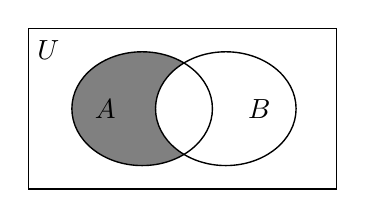
\begin{tikzpicture}[scale=0.85,line width=0.5pt]
\draw (0,0) rectangle (4.6,2.4);
\fill[gray] (1.7,1.2) ellipse (1.05 and 0.85);
\fill[white] (2.95,1.2) ellipse (1.05 and 0.85);
\draw (1.7,1.2) ellipse (1.05 and 0.85);
\draw (2.95,1.2) ellipse (1.05 and 0.85);
\node at (1.15,1.2) {$A$};
\node at (3.45,1.2) {$B$};
\node at (0.3,2.08) {$U$};
\end{tikzpicture}
\end{center}

\ifanswer
\solbegin
\step{$A=\{x\mid y=\sqrt{-x^2+x+2}\}=\{x\mid-1\leqslant x\leqslant2\}$，}
\step{$\overline B=\{x\mid 0\leqslant x\leqslant5\}$，$C=A\cap\overline B=[0,2]$.}
\solend
\fi

\item 关于 $x$ 的不等式 $ax-b<0$ 的解集为 $(2,+\infty)$，则关于 $x$ 的不等式 $(ax+b)(x-1)<0$ 的解集为\blankline[4.4em].

\ifanswer
\solbegin
\step{因为关于 $x$ 的不等式 $ax-b<0$ 的解集为 $(2,+\infty)$，所以 $\begin{cases}a<0\\2a-b=0\end{cases}$，}
\step{所以不等式 $(ax+b)(x-1)<0$ 可化为 $a\left(x+\dfrac ba\right)(x-1)<0$，$a<0$，}
\step{所以 $(x+2)(x-1)>0$，}
\step{所以所求解集为 $(-\infty,-2)\cup(1,+\infty)$.}
\solend
\fi

\item $a_1$、$b_1$、$a_2$、$b_2$ 均为非零实数，不等式 $a_1x+b_1>0$ 和 $a_2x+b_2>0$ 的解集分别为集合 $M$、$N$，那么“$\dfrac{a_1}{a_2}=\dfrac{b_1}{b_2}$”是“$M=N$”的\blankline[4.4em]条件（选填“充分非必要”、“必要非充分”、“充要”和“既非充分也非必要”）.

\ifanswer
\solbegin
\step{当 $a_1=b_1=1$，$a_2=b_2=-1$ 时，满足 $\dfrac{a_1}{a_2}=\dfrac{b_1}{b_2}$，}
\step{但是 $M=N$ 不成立，即充分性不成立；}
\step{若 $M=N$ 时，$\dfrac{a_1}{a_2}=\dfrac{b_1}{b_2}$ 一定成立，即必要性成立.}
\step{故为必要不充分条件.}% 原卷选项列“必要非充分”、解析结论作“必要不充分”，照录
\solend
\fi

\item 已知集合 $\{a,b,c\}=\{0,1,2\}$，且下列三个关系：① $a\neq2$；② $b=2$；③ $c\neq0$；有且只有一个正确，则 $100a+10b+c=$\blankline[4.4em].

\ifanswer
\solbegin
\step{列表如下：}
\begin{center}
\begin{tabular}{|c|c|c|c|c|}
\hline
 & ① & ② & ③ & \\
\hline
① 正确 & $a\neq2$ & $b\neq2$ & $c=0$ & 无解\\
\hline
② 正确 & $a=2$ & $b=2$ & $c=0$ & 矛盾\\
\hline
③ 正确 & $a=2$ & $b\neq2$ & $c\neq0$ & $a=2,b=0,c=1$\\
\hline
\end{tabular}
\end{center}
\step{所以 $100a+10b+c=201$.}
\solend
\fi

\end{enumerate}

\bigsec{二、选择题}

\begin{enumerate}
\setcounter{enumi}{12}

\item 已知 $a$,$b$,$c\in\R$,$b>c$，则下列不等式中恒成立的是\mbox{（\quad）}

\keepwithprev
A. $a+b^2>a+c^2$\qquad\quad B. $a^2+b>a^2+c$\qquad\quad C. $ab^2>ac^2$\qquad\quad D. $a^2b>a^2c$

\ifanswer
\solbegin
\step{对于 $A$，取 $b=1,c=-1$，错误；对于 $B$，由不等式的同向可加性得正确；}
\step{对于 $C$，取 $a=1,b=1,c=-2$，错误；对于 $D$，取 $a=0$，错误；}
\step{故选 $B$.}
\solend
\fi

\item 给出命题：“如果 $n$ 是素数，那么 $n^2+2$ 不是素数”，甲同学判断该命题是假命题，他做出这个判断的反例可以是\mbox{（\quad）}% 原卷把答案“$B$”印在题干括号内、无【解析】

\keepwithprev
A. $n=2$\qquad\quad B. $n=3$\qquad\quad C. $n=4$\qquad\quad D. $n=5$

\ifanswer
\ans{$B$}
\fi

\item 设集合 $A=\left\{x\,\middle\vert\,x=\dfrac n2,n\in\Z\right\}$，$B=\left\{x\,\middle\vert\,x=n+\dfrac12,n\in\Z\right\}$，则下列图形能表示 $A$ 与 $B$ 关系的是\mbox{（\quad）}

\keepwithprev
\begin{center}
% 原卷四个文氏图选项按原图形状用 TikZ 重排。
\begin{tabular}{c@{\qquad\qquad}c}
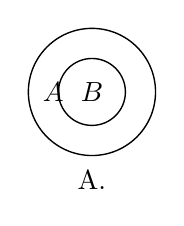
\begin{tikzpicture}[scale=0.85,line width=0.5pt]
\draw (0.9,0.9) circle (0.95);
\draw (0.9,0.9) circle (0.5);
\node at (0.32,0.9) {$A$};
\node at (0.9,0.9) {$B$};
\node[anchor=north] at (0.9,-0.12) {A.};
\end{tikzpicture}
&
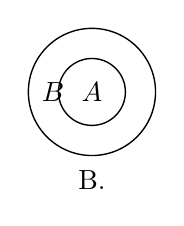
\begin{tikzpicture}[scale=0.85,line width=0.5pt]
\draw (0.9,0.9) circle (0.95);
\draw (0.9,0.9) circle (0.5);
\node at (0.32,0.9) {$B$};
\node at (0.9,0.9) {$A$};
\node[anchor=north] at (0.9,-0.12) {B.};
\end{tikzpicture}
\\[12pt]
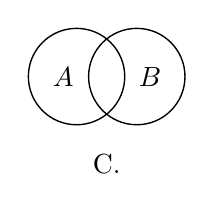
\begin{tikzpicture}[scale=0.85,line width=0.5pt]
\draw (0.65,0.9) circle (0.72);
\draw (1.55,0.9) circle (0.72);
\node at (0.45,0.9) {$A$};
\node at (1.75,0.9) {$B$};
\node[anchor=north] at (1.1,-0.12) {C.};
\end{tikzpicture}
&
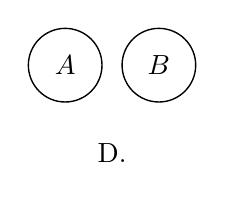
\begin{tikzpicture}[scale=0.85,line width=0.5pt]
\draw (0.55,0.9) circle (0.55);
\draw (1.95,0.9) circle (0.55);
\node at (0.55,0.9) {$A$};
\node at (1.95,0.9) {$B$};
\node[anchor=north] at (1.25,-0.12) {D.};
\end{tikzpicture}
\end{tabular}
\end{center}

\ifanswer
\solbegin
\step{$B\subset A$，图形能表示 $A$ 与 $B$ 关系的是 $A$. 故选 $A$.}
\solend
\fi

\item 以某些整数为元素的集合 $P$ 具有以下性质：

（1）$P$ 中元素有正数，也有负数；（2）$P$ 中元素有奇数，也有偶数；

（3）$-1\notin P$；（4）若 $x$、$y\in P$，则 $x+y\in P$.

则下列选项哪个是正确的\mbox{（\quad）}

\keepwithprev
A. 集合 $P$ 中一定有 $0$ 但没有 $2$\qquad\qquad B. 集合 $P$ 中一定有 $0$ 可能有 $2$

C. 集合 $P$ 中可能有 $0$ 可能有 $2$\qquad\qquad D. 集合 $P$ 中既没有 $0$ 又没有 $2$

\ifanswer
\solbegin
\step{由（4）得 $x\in P$，则 $kx\in P(k$ 是正整数$)$.}
\step{由（1）可设 $x$、$y\in P$，且 $x>0$，$y<0$，则 $xy$、$(-y)x\in P$，}
\step{因而 $0=xy+(-y)x\in P$.}
\step{假设 $2\in P$，则 $2k\in P$. 由上面及（4）得 $0$，$2$，$4$，$6$，$8$，$\cdots$ 均在 $P$ 中，}
\step{故 $2k-2\in P(k$ 是正整数$)$，}
\step{不妨令 $P$ 中负数为奇数 $-2k+1(k$ 为正整数$)$，}
\step{由（4）得 $(2k-2)+(-2k+1)=-1\in P$，矛盾.}
\step{故若 $2\in P$，则 $P$ 中没有负奇数.}
\step{若 $P$ 中负数为偶数，设为 $-2k(k$ 为正整数$)$，则由（4）及 $2\in P$，}
\step{得 $-2$,$-4$,$-6$,$\cdots$ 均在 $P$ 中，即 $-2m-2\in P(m$ 为非负整数$)$，}
\step{则 $P$ 中正奇数为 $2m+1$，由（4）得 $(-2m-2)+(2m+1)=-1\in P$，矛盾.}
\step{综上，$0\in P$，$2\notin P$，故选 $A$.}
\solend
\fi

\end{enumerate}

\bigsec{三、解答题}

\begin{enumerate}
\setcounter{enumi}{16}

\item （1）已知 $a$、$b$ 为实数，比较 $a^2+b^2$ 与 $4a-2b-5$ 的值的大小.

（2）若 $-1\leqslant x+y\leqslant2$，$-2\leqslant x-y\leqslant1$，求 $x-2y$ 的范围.

\ifanswer
\solbegin
\step{（1）$a^2+b^2-(4a-2b-5)=a^2-4a+4+b^2+2b+1=(a-2)^2+(b+1)^2\geqslant0$，}
\step{故 $a^2+b^2\geqslant4a-2b-5$.}
\step{（2）设 $x-2y=m(x+y)+n(x-y)$，则 $x-2y=(m+n)x+(m-n)y$，}
\step{所以 $\begin{cases}m+n=1\\m-n=-2\end{cases}$，解得 $n=\dfrac32$，$m=-\dfrac12$，}
\step{所以 $x-2y=-\dfrac12(x+y)+\dfrac32(x-y)$，}
\step{因为 $-1\leqslant x+y\leqslant2$，$-2\leqslant x-y\leqslant1$，}
\step{所以 $-1\leqslant-\dfrac12(x+y)\leqslant\dfrac12$，$-3\leqslant\dfrac32(x-y)\leqslant\dfrac32$，}
\step{所以 $-4\leqslant-\dfrac12(x+y)+\dfrac32(x-y)\leqslant2$，即 $-4\leqslant x-2y\leqslant2$，}
\step{故 $x-2y$ 的范围是 $[-4,2]$.}
\solend
\fi

\item 已知集合 $A=\{x\mid\lvert x-2\rvert<a\}$，集合 $B=\left\{x\,\middle\vert\,\dfrac{2x-1}{x+2}<1\right\}$.

（1）若 $a=2$，求 $A\cup B$,$A\cap B$；

（2）若 $A\cap B=A$，求实数 $a$ 的取值范围.

\ifanswer
\solbegin
\step{（1）由题意得 $A=(0,4)$,$B=(-2,3)$，所以 $A\cup B=(-2,4)$,$A\cap B=(0,3)$；}
\step{（2）因为 $A\cap B=A$，所以 $A\subseteq B$，}
\step{当 $a\leqslant0$ 时，$A=\varnothing$，满足 $A\subseteq B$；}
\step{当 $a>0$ 时，$A=(2-a,2+a)$,$B=(-2,3)$，}
\step{因为 $A\subseteq B$，所以 $\begin{cases}-2\leqslant2-a\\3\geqslant2+a\end{cases}$，解得 $a\leqslant1$，即 $0<a\leqslant1$.}
\step{因此，实数 $a$ 的取值范围为 $(-\infty,1]$.}
\solend
\fi

\item 我校校园文化节即将到来，高一年级将开展“数字配对”的抽奖活动，活动规则如下：每人可以抽取一张卡片，每张卡片上都印有一个不小于 $-10$ 且不大于 $10$ 的整数，其中不含 $2$. 每张卡片数字对应一个抽奖号码，卡片上的数字减去 $2$ 所得的差，与抽奖号码减去 $3$ 所得的差，两者的乘积等于 $12$.

（1）记卡片上的数字为 $x$，卡片数字对应的抽奖号码为 $y$，请用含有卡片数字 $x$ 的式子来表示抽奖号码 $y$；

（2）当抽奖号码不小于 $3$ 且不大于 $7$ 时，抽奖者可以领取奖品. 请问抽到哪些数字的卡片可以领取奖品？请写出满足领取奖品的卡片数字所组成的集合.

\ifanswer
\solbegin
\step{（1）卡片上的数字为 $x$，对应的抽奖号码为 $y$，}
\step{由题意得 $(x-2)(y-3)=12$，因为 $x\neq2$，所以 $y=3+\dfrac{12}{x-2}$，}
\step{所以 $y=3+\dfrac{12}{x-2}(-10\leqslant x\leqslant10,x\in\Z,x\neq2)$.}
\step{（2）由（1）得 $y=3+\dfrac{12}{x-2}(-10\leqslant x\leqslant10,x\in\Z,x\neq2)$，}
\step{由抽奖条件，得 $3\leqslant3+\dfrac{12}{x-2}\leqslant7$，$x\geqslant5$，所以 $5\leqslant x\leqslant10$，$x\in\Z$，}
\step{所以可领取奖品的卡片数字为 $\{5,6,7,8,9,10\}$.}
\solend
\fi

\item （1）已知 $m\in\R$，若不等式 $(m+1)x^2-mx+m-1<0$ 的解集是空集，求 $m$ 的取值范围；

（2）命题 $P:x^2-5x+6<0$，命题 $q:x^2-4ax+3a^2<0$，若命题 $P$ 是命题 $q$ 的充分非必要条件，求实数 $a$ 的取值范围.

\ifanswer
\solbegin
\step{（1）①当 $m+1=0$，即 $m=-1$ 时，$f(x)=x-2$，不合题意；}
\step{②当 $m+1\neq0$，即 $m\neq-1$ 时，$\begin{cases}m+1>0\\\Delta=m^2-4(m+1)(m-1)\leqslant0\end{cases}$，解得 $m\geqslant\dfrac{2\sqrt3}{3}$，}
\step{所以 $m$ 的取值范围是 $\left[\dfrac{2\sqrt3}{3},+\infty\right)$；}
\step{（2）解 $x^2-5x+6<0$，因式分解得 $(x-2)(x-3)<0$，故 $P$ 的解集为 $(2,3)$，}
\step{解 $x^2-4ax+3a^2<0$，因式分解得 $(x-a)(x-3a)<0$，}
\step{因为命题 $P$ 是命题 $q$ 的充分不必要条件，所以 $(2,3)$ 是 $q$ 解集的真子集，}
\step{当 $a=0$ 时，$q$ 的解集为 $\varnothing$，不合题意，舍去；}
\step{当 $a<0$ 时，$q$ 的解集为 $(3a,a)$，$\begin{cases}3a\leqslant2\\a\geqslant3\end{cases}$，不等式组无解，舍去；}
\step{当 $a>0$ 时，$q$ 的解集为 $(a,3a)$，又因为 $(2,3)$ 是 $q$ 解集的真子集，}
\step{所以 $\begin{cases}a\leqslant2\\3a\geqslant3\end{cases}$（等号不同时取），解得 $1\leqslant a\leqslant2$；}
\step{综上，实数 $a$ 的取值范围是 $[1,2]$.}
\solend
\fi

\item 对于至少含两个元素的有限正整数集 $A$，定义它的“两两和集”为
$S(A)=\{z\mid z=x+y$，其中 $x$、$y\in A$，且 $x<y\}$.

（1）若 $A=\{1,2,4,5\}$，求 $S(A)$；

（2）已知集合 $A$ 中恰好含有四个元素，且 $S(A)=\{5,7,8,10,11,13\}$，写出所有符合条件的集合 $A$；

（3）猜想：当集合 $A$ 含有 $n$ 个元素（$n\geqslant2$）时，$S(A)$ 的元素个数最少是多少？证明你的猜想.

\ifanswer
\solbegin
\step{（1）因为 $A=\{1,2,4,5\}$，计算所有两两和并去掉重复的结果有 $3$，$5$，$6$，$7$，$9$，}
\step{所以 $S(A)=\{3,5,6,7,9\}$.}
\step{（2）设 $A=\{a,b,c,d\}$，其中 $a<b<c<d$，且 $S(A)=\{5,7,8,10,11,13\}$，}
\step{四个元素共有六种两两配对，和集恰好有六个元素，}
\step{因此六个和互不相同.}
\step{这六个数分别为 $a+b$,$a+c$,$a+d$,$b+c$,$b+d$,$c+d$，}
\step{所以这六个数从小到大，可以确定第一个数为 $a+b$，第二数为 $a+c$，}
\step{第五个数为 $b+d$，第六数为 $c+d$，}
\step{第三个数和第四个数不能确定，即 $b+c$ 和 $a+d$ 的大小不定.}
\step{所以 $a+b=5$,$a+c=7$,$b+d=11$,$c+d=13$.}
\step{由此得到 $b=5-a$,$c=7-a$,$d=6+a$，}
\step{于是 $a+d=2a+6$,$b+c=12-2a$.}
\step{其余两个数 $b+c$,$a+d$ 对应 $8$,$10$，分两种情况讨论：}
\step{①若 $b+c=8$,$a+d=10$，则 $\begin{cases}12-2a=8\\2a+6=10\end{cases}$，解得 $a=2$，}
\step{所以 $A=\{2,3,5,8\}$；}
\step{②若 $b+c=10$,$a+d=8$，则 $\begin{cases}12-2a=10\\2a+6=8\end{cases}$，解得 $a=1$，}
\step{所以 $A=\{1,4,6,7\}$；}
\step{检验得，两组均符合题意.}
\step{因此所有符合条件的集合为 $A=\{1,4,6,7\}$ 或 $A=\{2,3,5,8\}$.}
\step{（3）猜想：两两和集的元素个数的最小值为 $2n-3$. 证明如下：}
\step{将集合中的元素按从小到大排列为 $a_1<a_2<\cdots<a_n$，}
\step{当 $n=2$ 时，两两和集恰好有一个元素，结论成立.}
\step{当 $n\geqslant3$ 时，考虑下列均属于 $S(A)$ 的数，}
\step{由不等式的传递性得严格不等式：}
\step{$a_1+a_2<a_1+a_3<\cdots<a_1+a_n<a_2+a_n<\cdots<a_{n-1}+a_n$，}
\step{其中 $a_1+a_2<a_1+a_3<\cdots<a_1+a_n$ 共有 $n-1$ 个不相等的数；}
\step{$a_2+a_n<\cdots<a_{n-1}+a_n$ 共有 $n-2$ 个不相等的数，}
\step{所以一共有 $(n-1)+(n-2)=2n-3$ 个，}
\step{因此，两两和集至少含有 $2n-3$ 个元素.}
\step{再证明可以取到 $2n-3$：}
\step{对任意 $n\geqslant2$，取 $A=\{1,2,\cdots,n\}$，}
\step{所有两两和都是不小于 $3$ 且不大于 $2n-1$ 的整数，}
\step{其中，$1+2$,$1+3$,$\cdots$,$1+n$ 是从 $3$ 到 $n+1$ 的整数；}
\step{当 $n\geqslant3$ 时，$2+n$,$3+n$,$\cdots$,$(n-1)+n$ 可取到其余整数；}
\step{因此 $S(A)=\{3,4,\cdots,2n-1\}$，其元素个数为 $(2n-1)-3+1=2n-3$，}
\step{所以所求最小值为 $2n-3$.}
\solend
\fi

\end{enumerate}

\end{document}
"
%
% 原始材料：微信公众号“魔都数学加油站”文章，作者破晓，2026-11-06 17:58 发布；
% 连载“27学年高一118”，原文标题“27学年高一118——2026-2027年上海市罗店中学高一上10月月考”；
% 原文链接：https://mp.weixin.qq.com/s/4edo8awYdjmWJl153X-aDA。
% 正文为 9 张 PNG 页（第 2、3、5、9 页 2560×3620，其余 4762×6735），
% 题目下印有【解析】或【答案】，为讲评版。
% 题目、解析均据原图转录；卷面红色水印及公众号页脚未录入。
%
% 卷首标题：原卷印作“2026-2027 年罗店中学高一上 10 月月考”（公众号标题中的“上海市”
% 卷面标题行没有，本稿照卷面），年份区间按全稿惯例排 en dash；原卷未印副标题，本稿按题目内容
% 标为“集合与常用逻辑用语、不等式”。
%
% 与原卷的排版差异：
%   ① 原文从第 3 题起，填空题 3—12、选择题 13—16、解答题 17—21，共 19 题，本稿保留原题号；
%   ② 原卷每题下直接印【解析】／【答案】，本稿按全稿惯例置于答案版；第 4 题只印【答案】、
%      第 14 题把答案“$B$”印在题干括号内且无【解析】，均另提 \ans{}；其余选择题答案在
%      解析末句“故选 …”，括号内留空；
%   ③ 原卷未印副标题，本稿按“知识模块”口径补出；
%   ④ 原卷填空横线按全稿惯例排为 \blankline[4.4em]；选择题括号排 \mbox{（\quad）}、
%      选项段前按惯例加 \keepwithprev；解答题不留作答区（原卷为讲评版，与 109—117 同）；
%   ⑤ 原卷数集 $R$／$Z$ 按全稿惯例改 \R、\Z，补集照原卷上划线排 \overline{B}。
%
% 子集符号：第 6 题、第 18 题的 $\{x\mid x<1\}\subseteq\{x\mid x<3a-2\}$ 与 $A\subseteq B$
%   印有下划线，照录 \subseteq；第 15 题解析的 $B\subset A$ 印单线（真子集、无下划线），
%   按 18／96 成例照录 \subset。
%
% 判别式字形：第 20 题 (1) cases 的判别式原卷排 $\Delta$（等腰、右厚），照录 \Delta。
%
% 图与表：第 9 题题干的文氏图（矩形 $U$ 内两椭圆 $A$、$B$，阴影为 $A\cap\overline B$）
%   按原图形状用 TikZ 重绘（三版都出）；第 12 题解析的“列表”按原卷用 tabular 重排
%   （仅答案版）；第 15 题四个文氏图选项按原图形状用 TikZ 重排（三版都出）。
%
% 原卷存疑照录：第 8 题解析“$2022+3\cdot1\cdot(-1)=2026$”一行、第 11 题解析结论
%   作“必要不充分条件”而选项列“必要非充分”、第 20 题 (2) 的 cases，均照录加注。
%
% 行数核对：逐题数 \step/\stepm 条数，合计 110 条（Q3：2；Q4：0；Q5：1；Q6：2；Q7：5；
% Q8：3；Q9：2；Q10：4；Q11：4；Q12：2；Q13：3；Q14：0；Q15：1；Q16：12；Q17：9；
% Q18：6；Q19：6；Q20：11；Q21：36），与原卷印刷行逐题相等（cases／tabular／TikZ
% 图块作一个印刷行计）。第 4 题只印【答案】、第 14 题括号内印答案且无解析，均提 \ans{}，
% 不计入 \step 账。
%
\documentclass[a4paper,11pt]{article}
\usepackage{common}

\begin{document}

\examtitlest[3]{2026--2027 年罗店中学高一上 10 月月考}{集合与常用逻辑用语、不等式}

\bigsec{一、填空题}

\begin{enumerate}
\setcounter{enumi}{2}

\item 若 $2x^2+3x+5=a(2x+1)(x+1)+b$ 恒成立，则 $a-b$ 的值\blankline[4.4em].

\ifanswer
\solbegin
\step{因为 $2x^2+3x+5=a(2x+1)(x+1)+b=2ax^2+3ax+a+b$ 恒成立，}
\step{所以 $\begin{cases}2=2a\\3=3a\\5=a+b\end{cases}$，所以 $\begin{cases}a=1\\b=4\end{cases}$，故 $a-b$ 的值为 $-3$.}
\solend
\fi

\item “$a$、$b$ 中至少有一个能被 $6$ 整除”的否定形式是\blankline[4.4em].

\ifanswer
\ans{$a$、$b$ 都不能被 $6$ 整除}
\fi

\item 设集合 $A=\{1,2\}$，则满足 $A\cup B=\{1,2,3\}$ 的集合 $B$ 的个数是\blankline[4.4em].

\ifanswer
\solbegin
\step{$B=\{3\}$,$\{1,3\}$,$\{2,3\}$,$\{1,2,3\}$，个数为 $4$.}
\solend
\fi

\item 命题“若 $x<1$，则 $x<3a-2$”是真命题，求实数 $a$ 的取值范围是\blankline[4.4em].

\ifanswer
\solbegin
\step{$\alpha:x<1$,$\beta:x<3a-2$，且若 $\alpha$ 则 $\beta$ 是真命题，}
\step{则 $\{x\mid x<1\}\subseteq\{x\mid x<3a-2\}$，所以 $3a-2\geqslant1$，解得 $a\geqslant1$.}
\solend
\fi

\item 不论实数 $m$ 取什么值，点 $P(m+1,2-m)$ 一定不在第\blankline[4.4em]象限（选填“一”、“二”、“三”或“四”）.

\ifanswer
\solbegin
\step{当 $m+1>0$，$2-m>0$ 时，解得 $-1<m<2$，此时点 $P$ 在第一象限；}
\step{当 $m+1<0$，$2-m>0$ 时，解得 $m<-1$，此时点 $P$ 在第二象限；}
\step{当 $m+1<0$，$2-m<0$ 时，$m$ 无解，此时点 $P$ 不可能在第三象限；}
\step{当 $m+1>0$，$2-m<0$ 时，解得 $m>2$，此时点 $P$ 在第四象限.}
\step{故一定不在第三象限.}
\solend
\fi

\item 设 $x_1$、$x_2$ 是方程 $x^2+x-3=0$ 的两个实数根，则 $x_1^2-x_2+2022=$\blankline[4.4em].

\ifanswer
\solbegin
\step{$x_1$、$x_2$ 是方程 $x^2+x-3=0$ 的两个实数根，}
\step{得 $x_1+x_2=-1$，$x_1^2+x_1-3=0$，所以 $x_1^2=3-x_1$，}
\step{$x_1^2-x_2+2022=3-x_1-x_2+2022=2022+3\cdot1\cdot(-1)=2026$.}
\solend
\fi

\item 如图，已知全集 $U=\R$，集合 $A=\{x\mid y=\sqrt{-x^2+x+2}\}$，$B=\{x\mid x<0$ 或 $x>5\}$. 集合 $C$ 表示图中阴影区域对应的集合，则集合 $C=$\blankline[4.4em]（用区间表示）.

\begin{center}
% 原卷文氏图：矩形 U 内两椭圆 A（阴影）、B，阴影为 A\cap\overline B，按原图形状用 TikZ 重绘。
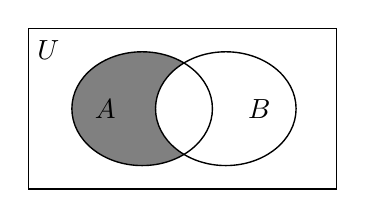
\begin{tikzpicture}[scale=0.85,line width=0.5pt]
\draw (0,0) rectangle (4.6,2.4);
\fill[gray] (1.7,1.2) ellipse (1.05 and 0.85);
\fill[white] (2.95,1.2) ellipse (1.05 and 0.85);
\draw (1.7,1.2) ellipse (1.05 and 0.85);
\draw (2.95,1.2) ellipse (1.05 and 0.85);
\node at (1.15,1.2) {$A$};
\node at (3.45,1.2) {$B$};
\node at (0.3,2.08) {$U$};
\end{tikzpicture}
\end{center}

\ifanswer
\solbegin
\step{$A=\{x\mid y=\sqrt{-x^2+x+2}\}=\{x\mid-1\leqslant x\leqslant2\}$，}
\step{$\overline B=\{x\mid 0\leqslant x\leqslant5\}$，$C=A\cap\overline B=[0,2]$.}
\solend
\fi

\item 关于 $x$ 的不等式 $ax-b<0$ 的解集为 $(2,+\infty)$，则关于 $x$ 的不等式 $(ax+b)(x-1)<0$ 的解集为\blankline[4.4em].

\ifanswer
\solbegin
\step{因为关于 $x$ 的不等式 $ax-b<0$ 的解集为 $(2,+\infty)$，所以 $\begin{cases}a<0\\2a-b=0\end{cases}$，}
\step{所以不等式 $(ax+b)(x-1)<0$ 可化为 $a\left(x+\dfrac ba\right)(x-1)<0$，$a<0$，}
\step{所以 $(x+2)(x-1)>0$，}
\step{所以所求解集为 $(-\infty,-2)\cup(1,+\infty)$.}
\solend
\fi

\item $a_1$、$b_1$、$a_2$、$b_2$ 均为非零实数，不等式 $a_1x+b_1>0$ 和 $a_2x+b_2>0$ 的解集分别为集合 $M$、$N$，那么“$\dfrac{a_1}{a_2}=\dfrac{b_1}{b_2}$”是“$M=N$”的\blankline[4.4em]条件（选填“充分非必要”、“必要非充分”、“充要”和“既非充分也非必要”）.

\ifanswer
\solbegin
\step{当 $a_1=b_1=1$，$a_2=b_2=-1$ 时，满足 $\dfrac{a_1}{a_2}=\dfrac{b_1}{b_2}$，}
\step{但是 $M=N$ 不成立，即充分性不成立；}
\step{若 $M=N$ 时，$\dfrac{a_1}{a_2}=\dfrac{b_1}{b_2}$ 一定成立，即必要性成立.}
\step{故为必要不充分条件.}% 原卷选项列“必要非充分”、解析结论作“必要不充分”，照录
\solend
\fi

\item 已知集合 $\{a,b,c\}=\{0,1,2\}$，且下列三个关系：① $a\neq2$；② $b=2$；③ $c\neq0$；有且只有一个正确，则 $100a+10b+c=$\blankline[4.4em].

\ifanswer
\solbegin
\step{列表如下：}
\begin{center}
\begin{tabular}{|c|c|c|c|c|}
\hline
 & ① & ② & ③ & \\
\hline
① 正确 & $a\neq2$ & $b\neq2$ & $c=0$ & 无解\\
\hline
② 正确 & $a=2$ & $b=2$ & $c=0$ & 矛盾\\
\hline
③ 正确 & $a=2$ & $b\neq2$ & $c\neq0$ & $a=2,b=0,c=1$\\
\hline
\end{tabular}
\end{center}
\step{所以 $100a+10b+c=201$.}
\solend
\fi

\end{enumerate}

\bigsec{二、选择题}

\begin{enumerate}
\setcounter{enumi}{12}

\item 已知 $a$,$b$,$c\in\R$,$b>c$，则下列不等式中恒成立的是\mbox{（\quad）}

\keepwithprev
A. $a+b^2>a+c^2$\qquad\quad B. $a^2+b>a^2+c$\qquad\quad C. $ab^2>ac^2$\qquad\quad D. $a^2b>a^2c$

\ifanswer
\solbegin
\step{对于 $A$，取 $b=1,c=-1$，错误；对于 $B$，由不等式的同向可加性得正确；}
\step{对于 $C$，取 $a=1,b=1,c=-2$，错误；对于 $D$，取 $a=0$，错误；}
\step{故选 $B$.}
\solend
\fi

\item 给出命题：“如果 $n$ 是素数，那么 $n^2+2$ 不是素数”，甲同学判断该命题是假命题，他做出这个判断的反例可以是\mbox{（\quad）}% 原卷把答案“$B$”印在题干括号内、无【解析】

\keepwithprev
A. $n=2$\qquad\quad B. $n=3$\qquad\quad C. $n=4$\qquad\quad D. $n=5$

\ifanswer
\ans{$B$}
\fi

\item 设集合 $A=\left\{x\,\middle\vert\,x=\dfrac n2,n\in\Z\right\}$，$B=\left\{x\,\middle\vert\,x=n+\dfrac12,n\in\Z\right\}$，则下列图形能表示 $A$ 与 $B$ 关系的是\mbox{（\quad）}

\keepwithprev
\begin{center}
% 原卷四个文氏图选项按原图形状用 TikZ 重排。
\begin{tabular}{c@{\qquad\qquad}c}
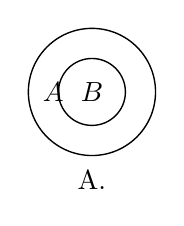
\begin{tikzpicture}[scale=0.85,line width=0.5pt]
\draw (0.9,0.9) circle (0.95);
\draw (0.9,0.9) circle (0.5);
\node at (0.32,0.9) {$A$};
\node at (0.9,0.9) {$B$};
\node[anchor=north] at (0.9,-0.12) {A.};
\end{tikzpicture}
&
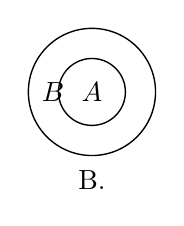
\begin{tikzpicture}[scale=0.85,line width=0.5pt]
\draw (0.9,0.9) circle (0.95);
\draw (0.9,0.9) circle (0.5);
\node at (0.32,0.9) {$B$};
\node at (0.9,0.9) {$A$};
\node[anchor=north] at (0.9,-0.12) {B.};
\end{tikzpicture}
\\[12pt]
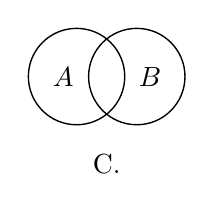
\begin{tikzpicture}[scale=0.85,line width=0.5pt]
\draw (0.65,0.9) circle (0.72);
\draw (1.55,0.9) circle (0.72);
\node at (0.45,0.9) {$A$};
\node at (1.75,0.9) {$B$};
\node[anchor=north] at (1.1,-0.12) {C.};
\end{tikzpicture}
&
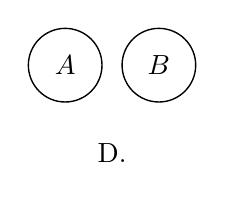
\begin{tikzpicture}[scale=0.85,line width=0.5pt]
\draw (0.55,0.9) circle (0.55);
\draw (1.95,0.9) circle (0.55);
\node at (0.55,0.9) {$A$};
\node at (1.95,0.9) {$B$};
\node[anchor=north] at (1.25,-0.12) {D.};
\end{tikzpicture}
\end{tabular}
\end{center}

\ifanswer
\solbegin
\step{$B\subset A$，图形能表示 $A$ 与 $B$ 关系的是 $A$. 故选 $A$.}
\solend
\fi

\item 以某些整数为元素的集合 $P$ 具有以下性质：

（1）$P$ 中元素有正数，也有负数；（2）$P$ 中元素有奇数，也有偶数；

（3）$-1\notin P$；（4）若 $x$、$y\in P$，则 $x+y\in P$.

则下列选项哪个是正确的\mbox{（\quad）}

\keepwithprev
A. 集合 $P$ 中一定有 $0$ 但没有 $2$\qquad\qquad B. 集合 $P$ 中一定有 $0$ 可能有 $2$

C. 集合 $P$ 中可能有 $0$ 可能有 $2$\qquad\qquad D. 集合 $P$ 中既没有 $0$ 又没有 $2$

\ifanswer
\solbegin
\step{由（4）得 $x\in P$，则 $kx\in P(k$ 是正整数$)$.}
\step{由（1）可设 $x$、$y\in P$，且 $x>0$，$y<0$，则 $xy$、$(-y)x\in P$，}
\step{因而 $0=xy+(-y)x\in P$.}
\step{假设 $2\in P$，则 $2k\in P$. 由上面及（4）得 $0$，$2$，$4$，$6$，$8$，$\cdots$ 均在 $P$ 中，}
\step{故 $2k-2\in P(k$ 是正整数$)$，}
\step{不妨令 $P$ 中负数为奇数 $-2k+1(k$ 为正整数$)$，}
\step{由（4）得 $(2k-2)+(-2k+1)=-1\in P$，矛盾.}
\step{故若 $2\in P$，则 $P$ 中没有负奇数.}
\step{若 $P$ 中负数为偶数，设为 $-2k(k$ 为正整数$)$，则由（4）及 $2\in P$，}
\step{得 $-2$,$-4$,$-6$,$\cdots$ 均在 $P$ 中，即 $-2m-2\in P(m$ 为非负整数$)$，}
\step{则 $P$ 中正奇数为 $2m+1$，由（4）得 $(-2m-2)+(2m+1)=-1\in P$，矛盾.}
\step{综上，$0\in P$，$2\notin P$，故选 $A$.}
\solend
\fi

\end{enumerate}

\bigsec{三、解答题}

\begin{enumerate}
\setcounter{enumi}{16}

\item （1）已知 $a$、$b$ 为实数，比较 $a^2+b^2$ 与 $4a-2b-5$ 的值的大小.

（2）若 $-1\leqslant x+y\leqslant2$，$-2\leqslant x-y\leqslant1$，求 $x-2y$ 的范围.

\ifanswer
\solbegin
\step{（1）$a^2+b^2-(4a-2b-5)=a^2-4a+4+b^2+2b+1=(a-2)^2+(b+1)^2\geqslant0$，}
\step{故 $a^2+b^2\geqslant4a-2b-5$.}
\step{（2）设 $x-2y=m(x+y)+n(x-y)$，则 $x-2y=(m+n)x+(m-n)y$，}
\step{所以 $\begin{cases}m+n=1\\m-n=-2\end{cases}$，解得 $n=\dfrac32$，$m=-\dfrac12$，}
\step{所以 $x-2y=-\dfrac12(x+y)+\dfrac32(x-y)$，}
\step{因为 $-1\leqslant x+y\leqslant2$，$-2\leqslant x-y\leqslant1$，}
\step{所以 $-1\leqslant-\dfrac12(x+y)\leqslant\dfrac12$，$-3\leqslant\dfrac32(x-y)\leqslant\dfrac32$，}
\step{所以 $-4\leqslant-\dfrac12(x+y)+\dfrac32(x-y)\leqslant2$，即 $-4\leqslant x-2y\leqslant2$，}
\step{故 $x-2y$ 的范围是 $[-4,2]$.}
\solend
\fi

\item 已知集合 $A=\{x\mid\lvert x-2\rvert<a\}$，集合 $B=\left\{x\,\middle\vert\,\dfrac{2x-1}{x+2}<1\right\}$.

（1）若 $a=2$，求 $A\cup B$,$A\cap B$；

（2）若 $A\cap B=A$，求实数 $a$ 的取值范围.

\ifanswer
\solbegin
\step{（1）由题意得 $A=(0,4)$,$B=(-2,3)$，所以 $A\cup B=(-2,4)$,$A\cap B=(0,3)$；}
\step{（2）因为 $A\cap B=A$，所以 $A\subseteq B$，}
\step{当 $a\leqslant0$ 时，$A=\varnothing$，满足 $A\subseteq B$；}
\step{当 $a>0$ 时，$A=(2-a,2+a)$,$B=(-2,3)$，}
\step{因为 $A\subseteq B$，所以 $\begin{cases}-2\leqslant2-a\\3\geqslant2+a\end{cases}$，解得 $a\leqslant1$，即 $0<a\leqslant1$.}
\step{因此，实数 $a$ 的取值范围为 $(-\infty,1]$.}
\solend
\fi

\item 我校校园文化节即将到来，高一年级将开展“数字配对”的抽奖活动，活动规则如下：每人可以抽取一张卡片，每张卡片上都印有一个不小于 $-10$ 且不大于 $10$ 的整数，其中不含 $2$. 每张卡片数字对应一个抽奖号码，卡片上的数字减去 $2$ 所得的差，与抽奖号码减去 $3$ 所得的差，两者的乘积等于 $12$.

（1）记卡片上的数字为 $x$，卡片数字对应的抽奖号码为 $y$，请用含有卡片数字 $x$ 的式子来表示抽奖号码 $y$；

（2）当抽奖号码不小于 $3$ 且不大于 $7$ 时，抽奖者可以领取奖品. 请问抽到哪些数字的卡片可以领取奖品？请写出满足领取奖品的卡片数字所组成的集合.

\ifanswer
\solbegin
\step{（1）卡片上的数字为 $x$，对应的抽奖号码为 $y$，}
\step{由题意得 $(x-2)(y-3)=12$，因为 $x\neq2$，所以 $y=3+\dfrac{12}{x-2}$，}
\step{所以 $y=3+\dfrac{12}{x-2}(-10\leqslant x\leqslant10,x\in\Z,x\neq2)$.}
\step{（2）由（1）得 $y=3+\dfrac{12}{x-2}(-10\leqslant x\leqslant10,x\in\Z,x\neq2)$，}
\step{由抽奖条件，得 $3\leqslant3+\dfrac{12}{x-2}\leqslant7$，$x\geqslant5$，所以 $5\leqslant x\leqslant10$，$x\in\Z$，}
\step{所以可领取奖品的卡片数字为 $\{5,6,7,8,9,10\}$.}
\solend
\fi

\item （1）已知 $m\in\R$，若不等式 $(m+1)x^2-mx+m-1<0$ 的解集是空集，求 $m$ 的取值范围；

（2）命题 $P:x^2-5x+6<0$，命题 $q:x^2-4ax+3a^2<0$，若命题 $P$ 是命题 $q$ 的充分非必要条件，求实数 $a$ 的取值范围.

\ifanswer
\solbegin
\step{（1）①当 $m+1=0$，即 $m=-1$ 时，$f(x)=x-2$，不合题意；}
\step{②当 $m+1\neq0$，即 $m\neq-1$ 时，$\begin{cases}m+1>0\\\Delta=m^2-4(m+1)(m-1)\leqslant0\end{cases}$，解得 $m\geqslant\dfrac{2\sqrt3}{3}$，}
\step{所以 $m$ 的取值范围是 $\left[\dfrac{2\sqrt3}{3},+\infty\right)$；}
\step{（2）解 $x^2-5x+6<0$，因式分解得 $(x-2)(x-3)<0$，故 $P$ 的解集为 $(2,3)$，}
\step{解 $x^2-4ax+3a^2<0$，因式分解得 $(x-a)(x-3a)<0$，}
\step{因为命题 $P$ 是命题 $q$ 的充分不必要条件，所以 $(2,3)$ 是 $q$ 解集的真子集，}
\step{当 $a=0$ 时，$q$ 的解集为 $\varnothing$，不合题意，舍去；}
\step{当 $a<0$ 时，$q$ 的解集为 $(3a,a)$，$\begin{cases}3a\leqslant2\\a\geqslant3\end{cases}$，不等式组无解，舍去；}
\step{当 $a>0$ 时，$q$ 的解集为 $(a,3a)$，又因为 $(2,3)$ 是 $q$ 解集的真子集，}
\step{所以 $\begin{cases}a\leqslant2\\3a\geqslant3\end{cases}$（等号不同时取），解得 $1\leqslant a\leqslant2$；}
\step{综上，实数 $a$ 的取值范围是 $[1,2]$.}
\solend
\fi

\item 对于至少含两个元素的有限正整数集 $A$，定义它的“两两和集”为
$S(A)=\{z\mid z=x+y$，其中 $x$、$y\in A$，且 $x<y\}$.

（1）若 $A=\{1,2,4,5\}$，求 $S(A)$；

（2）已知集合 $A$ 中恰好含有四个元素，且 $S(A)=\{5,7,8,10,11,13\}$，写出所有符合条件的集合 $A$；

（3）猜想：当集合 $A$ 含有 $n$ 个元素（$n\geqslant2$）时，$S(A)$ 的元素个数最少是多少？证明你的猜想.

\ifanswer
\solbegin
\step{（1）因为 $A=\{1,2,4,5\}$，计算所有两两和并去掉重复的结果有 $3$，$5$，$6$，$7$，$9$，}
\step{所以 $S(A)=\{3,5,6,7,9\}$.}
\step{（2）设 $A=\{a,b,c,d\}$，其中 $a<b<c<d$，且 $S(A)=\{5,7,8,10,11,13\}$，}
\step{四个元素共有六种两两配对，和集恰好有六个元素，}
\step{因此六个和互不相同.}
\step{这六个数分别为 $a+b$,$a+c$,$a+d$,$b+c$,$b+d$,$c+d$，}
\step{所以这六个数从小到大，可以确定第一个数为 $a+b$，第二数为 $a+c$，}
\step{第五个数为 $b+d$，第六数为 $c+d$，}
\step{第三个数和第四个数不能确定，即 $b+c$ 和 $a+d$ 的大小不定.}
\step{所以 $a+b=5$,$a+c=7$,$b+d=11$,$c+d=13$.}
\step{由此得到 $b=5-a$,$c=7-a$,$d=6+a$，}
\step{于是 $a+d=2a+6$,$b+c=12-2a$.}
\step{其余两个数 $b+c$,$a+d$ 对应 $8$,$10$，分两种情况讨论：}
\step{①若 $b+c=8$,$a+d=10$，则 $\begin{cases}12-2a=8\\2a+6=10\end{cases}$，解得 $a=2$，}
\step{所以 $A=\{2,3,5,8\}$；}
\step{②若 $b+c=10$,$a+d=8$，则 $\begin{cases}12-2a=10\\2a+6=8\end{cases}$，解得 $a=1$，}
\step{所以 $A=\{1,4,6,7\}$；}
\step{检验得，两组均符合题意.}
\step{因此所有符合条件的集合为 $A=\{1,4,6,7\}$ 或 $A=\{2,3,5,8\}$.}
\step{（3）猜想：两两和集的元素个数的最小值为 $2n-3$. 证明如下：}
\step{将集合中的元素按从小到大排列为 $a_1<a_2<\cdots<a_n$，}
\step{当 $n=2$ 时，两两和集恰好有一个元素，结论成立.}
\step{当 $n\geqslant3$ 时，考虑下列均属于 $S(A)$ 的数，}
\step{由不等式的传递性得严格不等式：}
\step{$a_1+a_2<a_1+a_3<\cdots<a_1+a_n<a_2+a_n<\cdots<a_{n-1}+a_n$，}
\step{其中 $a_1+a_2<a_1+a_3<\cdots<a_1+a_n$ 共有 $n-1$ 个不相等的数；}
\step{$a_2+a_n<\cdots<a_{n-1}+a_n$ 共有 $n-2$ 个不相等的数，}
\step{所以一共有 $(n-1)+(n-2)=2n-3$ 个，}
\step{因此，两两和集至少含有 $2n-3$ 个元素.}
\step{再证明可以取到 $2n-3$：}
\step{对任意 $n\geqslant2$，取 $A=\{1,2,\cdots,n\}$，}
\step{所有两两和都是不小于 $3$ 且不大于 $2n-1$ 的整数，}
\step{其中，$1+2$,$1+3$,$\cdots$,$1+n$ 是从 $3$ 到 $n+1$ 的整数；}
\step{当 $n\geqslant3$ 时，$2+n$,$3+n$,$\cdots$,$(n-1)+n$ 可取到其余整数；}
\step{因此 $S(A)=\{3,4,\cdots,2n-1\}$，其元素个数为 $(2n-1)-3+1=2n-3$，}
\step{所以所求最小值为 $2n-3$.}
\solend
\fi

\end{enumerate}

\end{document}
"
%
% 原始材料：微信公众号“魔都数学加油站”文章，作者破晓，2026-11-06 17:58 发布；
% 连载“27学年高一118”，原文标题“27学年高一118——2026-2027年上海市罗店中学高一上10月月考”；
% 原文链接：https://mp.weixin.qq.com/s/4edo8awYdjmWJl153X-aDA。
% 正文为 9 张 PNG 页（第 2、3、5、9 页 2560×3620，其余 4762×6735），
% 题目下印有【解析】或【答案】，为讲评版。
% 题目、解析均据原图转录；卷面红色水印及公众号页脚未录入。
%
% 卷首标题：原卷印作“2026-2027 年罗店中学高一上 10 月月考”（公众号标题中的“上海市”
% 卷面标题行没有，本稿照卷面），年份区间按全稿惯例排 en dash；原卷未印副标题，本稿按题目内容
% 标为“集合与常用逻辑用语、不等式”。
%
% 与原卷的排版差异：
%   ① 原文从第 3 题起，填空题 3—12、选择题 13—16、解答题 17—21，共 19 题，本稿保留原题号；
%   ② 原卷每题下直接印【解析】／【答案】，本稿按全稿惯例置于答案版；第 4 题只印【答案】、
%      第 14 题把答案“$B$”印在题干括号内且无【解析】，均另提 \ans{}；其余选择题答案在
%      解析末句“故选 …”，括号内留空；
%   ③ 原卷未印副标题，本稿按“知识模块”口径补出；
%   ④ 原卷填空横线按全稿惯例排为 \blankline[4.4em]；选择题括号排 \mbox{（\quad）}、
%      选项段前按惯例加 \keepwithprev；解答题不留作答区（原卷为讲评版，与 109—117 同）；
%   ⑤ 原卷数集 $R$／$Z$ 按全稿惯例改 \R、\Z，补集照原卷上划线排 \overline{B}。
%
% 子集符号：第 6 题、第 18 题的 $\{x\mid x<1\}\subseteq\{x\mid x<3a-2\}$ 与 $A\subseteq B$
%   印有下划线，照录 \subseteq；第 15 题解析的 $B\subset A$ 印单线（真子集、无下划线），
%   按 18／96 成例照录 \subset。
%
% 判别式字形：第 20 题 (1) cases 的判别式原卷排 $\Delta$（等腰、右厚），照录 \Delta。
%
% 图与表：第 9 题题干的文氏图（矩形 $U$ 内两椭圆 $A$、$B$，阴影为 $A\cap\overline B$）
%   按原图形状用 TikZ 重绘（三版都出）；第 12 题解析的“列表”按原卷用 tabular 重排
%   （仅答案版）；第 15 题四个文氏图选项按原图形状用 TikZ 重排（三版都出）。
%
% 原卷存疑照录：第 8 题解析“$2022+3\cdot1\cdot(-1)=2026$”一行、第 11 题解析结论
%   作“必要不充分条件”而选项列“必要非充分”、第 20 题 (2) 的 cases，均照录加注。
%
% 行数核对：逐题数 \step/\stepm 条数，合计 110 条（Q3：2；Q4：0；Q5：1；Q6：2；Q7：5；
% Q8：3；Q9：2；Q10：4；Q11：4；Q12：2；Q13：3；Q14：0；Q15：1；Q16：12；Q17：9；
% Q18：6；Q19：6；Q20：11；Q21：36），与原卷印刷行逐题相等（cases／tabular／TikZ
% 图块作一个印刷行计）。第 4 题只印【答案】、第 14 题括号内印答案且无解析，均提 \ans{}，
% 不计入 \step 账。
%
\documentclass[a4paper,11pt]{article}
\usepackage{common}

\begin{document}

\examtitlest[3]{2026--2027 年罗店中学高一上 10 月月考}{集合与常用逻辑用语、不等式}

\bigsec{一、填空题}

\begin{enumerate}
\setcounter{enumi}{2}

\item 若 $2x^2+3x+5=a(2x+1)(x+1)+b$ 恒成立，则 $a-b$ 的值\blankline[4.4em].

\ifanswer
\solbegin
\step{因为 $2x^2+3x+5=a(2x+1)(x+1)+b=2ax^2+3ax+a+b$ 恒成立，}
\step{所以 $\begin{cases}2=2a\\3=3a\\5=a+b\end{cases}$，所以 $\begin{cases}a=1\\b=4\end{cases}$，故 $a-b$ 的值为 $-3$.}
\solend
\fi

\item “$a$、$b$ 中至少有一个能被 $6$ 整除”的否定形式是\blankline[4.4em].

\ifanswer
\ans{$a$、$b$ 都不能被 $6$ 整除}
\fi

\item 设集合 $A=\{1,2\}$，则满足 $A\cup B=\{1,2,3\}$ 的集合 $B$ 的个数是\blankline[4.4em].

\ifanswer
\solbegin
\step{$B=\{3\}$,$\{1,3\}$,$\{2,3\}$,$\{1,2,3\}$，个数为 $4$.}
\solend
\fi

\item 命题“若 $x<1$，则 $x<3a-2$”是真命题，求实数 $a$ 的取值范围是\blankline[4.4em].

\ifanswer
\solbegin
\step{$\alpha:x<1$,$\beta:x<3a-2$，且若 $\alpha$ 则 $\beta$ 是真命题，}
\step{则 $\{x\mid x<1\}\subseteq\{x\mid x<3a-2\}$，所以 $3a-2\geqslant1$，解得 $a\geqslant1$.}
\solend
\fi

\item 不论实数 $m$ 取什么值，点 $P(m+1,2-m)$ 一定不在第\blankline[4.4em]象限（选填“一”、“二”、“三”或“四”）.

\ifanswer
\solbegin
\step{当 $m+1>0$，$2-m>0$ 时，解得 $-1<m<2$，此时点 $P$ 在第一象限；}
\step{当 $m+1<0$，$2-m>0$ 时，解得 $m<-1$，此时点 $P$ 在第二象限；}
\step{当 $m+1<0$，$2-m<0$ 时，$m$ 无解，此时点 $P$ 不可能在第三象限；}
\step{当 $m+1>0$，$2-m<0$ 时，解得 $m>2$，此时点 $P$ 在第四象限.}
\step{故一定不在第三象限.}
\solend
\fi

\item 设 $x_1$、$x_2$ 是方程 $x^2+x-3=0$ 的两个实数根，则 $x_1^2-x_2+2022=$\blankline[4.4em].

\ifanswer
\solbegin
\step{$x_1$、$x_2$ 是方程 $x^2+x-3=0$ 的两个实数根，}
\step{得 $x_1+x_2=-1$，$x_1^2+x_1-3=0$，所以 $x_1^2=3-x_1$，}
\step{$x_1^2-x_2+2022=3-x_1-x_2+2022=2022+3\cdot1\cdot(-1)=2026$.}
\solend
\fi

\item 如图，已知全集 $U=\R$，集合 $A=\{x\mid y=\sqrt{-x^2+x+2}\}$，$B=\{x\mid x<0$ 或 $x>5\}$. 集合 $C$ 表示图中阴影区域对应的集合，则集合 $C=$\blankline[4.4em]（用区间表示）.

\begin{center}
% 原卷文氏图：矩形 U 内两椭圆 A（阴影）、B，阴影为 A\cap\overline B，按原图形状用 TikZ 重绘。
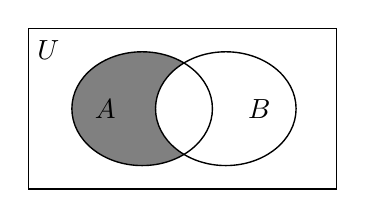
\begin{tikzpicture}[scale=0.85,line width=0.5pt]
\draw (0,0) rectangle (4.6,2.4);
\fill[gray] (1.7,1.2) ellipse (1.05 and 0.85);
\fill[white] (2.95,1.2) ellipse (1.05 and 0.85);
\draw (1.7,1.2) ellipse (1.05 and 0.85);
\draw (2.95,1.2) ellipse (1.05 and 0.85);
\node at (1.15,1.2) {$A$};
\node at (3.45,1.2) {$B$};
\node at (0.3,2.08) {$U$};
\end{tikzpicture}
\end{center}

\ifanswer
\solbegin
\step{$A=\{x\mid y=\sqrt{-x^2+x+2}\}=\{x\mid-1\leqslant x\leqslant2\}$，}
\step{$\overline B=\{x\mid 0\leqslant x\leqslant5\}$，$C=A\cap\overline B=[0,2]$.}
\solend
\fi

\item 关于 $x$ 的不等式 $ax-b<0$ 的解集为 $(2,+\infty)$，则关于 $x$ 的不等式 $(ax+b)(x-1)<0$ 的解集为\blankline[4.4em].

\ifanswer
\solbegin
\step{因为关于 $x$ 的不等式 $ax-b<0$ 的解集为 $(2,+\infty)$，所以 $\begin{cases}a<0\\2a-b=0\end{cases}$，}
\step{所以不等式 $(ax+b)(x-1)<0$ 可化为 $a\left(x+\dfrac ba\right)(x-1)<0$，$a<0$，}
\step{所以 $(x+2)(x-1)>0$，}
\step{所以所求解集为 $(-\infty,-2)\cup(1,+\infty)$.}
\solend
\fi

\item $a_1$、$b_1$、$a_2$、$b_2$ 均为非零实数，不等式 $a_1x+b_1>0$ 和 $a_2x+b_2>0$ 的解集分别为集合 $M$、$N$，那么“$\dfrac{a_1}{a_2}=\dfrac{b_1}{b_2}$”是“$M=N$”的\blankline[4.4em]条件（选填“充分非必要”、“必要非充分”、“充要”和“既非充分也非必要”）.

\ifanswer
\solbegin
\step{当 $a_1=b_1=1$，$a_2=b_2=-1$ 时，满足 $\dfrac{a_1}{a_2}=\dfrac{b_1}{b_2}$，}
\step{但是 $M=N$ 不成立，即充分性不成立；}
\step{若 $M=N$ 时，$\dfrac{a_1}{a_2}=\dfrac{b_1}{b_2}$ 一定成立，即必要性成立.}
\step{故为必要不充分条件.}% 原卷选项列“必要非充分”、解析结论作“必要不充分”，照录
\solend
\fi

\item 已知集合 $\{a,b,c\}=\{0,1,2\}$，且下列三个关系：① $a\neq2$；② $b=2$；③ $c\neq0$；有且只有一个正确，则 $100a+10b+c=$\blankline[4.4em].

\ifanswer
\solbegin
\step{列表如下：}
\begin{center}
\begin{tabular}{|c|c|c|c|c|}
\hline
 & ① & ② & ③ & \\
\hline
① 正确 & $a\neq2$ & $b\neq2$ & $c=0$ & 无解\\
\hline
② 正确 & $a=2$ & $b=2$ & $c=0$ & 矛盾\\
\hline
③ 正确 & $a=2$ & $b\neq2$ & $c\neq0$ & $a=2,b=0,c=1$\\
\hline
\end{tabular}
\end{center}
\step{所以 $100a+10b+c=201$.}
\solend
\fi

\end{enumerate}

\bigsec{二、选择题}

\begin{enumerate}
\setcounter{enumi}{12}

\item 已知 $a$,$b$,$c\in\R$,$b>c$，则下列不等式中恒成立的是\mbox{（\quad）}

\keepwithprev
A. $a+b^2>a+c^2$\qquad\quad B. $a^2+b>a^2+c$\qquad\quad C. $ab^2>ac^2$\qquad\quad D. $a^2b>a^2c$

\ifanswer
\solbegin
\step{对于 $A$，取 $b=1,c=-1$，错误；对于 $B$，由不等式的同向可加性得正确；}
\step{对于 $C$，取 $a=1,b=1,c=-2$，错误；对于 $D$，取 $a=0$，错误；}
\step{故选 $B$.}
\solend
\fi

\item 给出命题：“如果 $n$ 是素数，那么 $n^2+2$ 不是素数”，甲同学判断该命题是假命题，他做出这个判断的反例可以是\mbox{（\quad）}% 原卷把答案“$B$”印在题干括号内、无【解析】

\keepwithprev
A. $n=2$\qquad\quad B. $n=3$\qquad\quad C. $n=4$\qquad\quad D. $n=5$

\ifanswer
\ans{$B$}
\fi

\item 设集合 $A=\left\{x\,\middle\vert\,x=\dfrac n2,n\in\Z\right\}$，$B=\left\{x\,\middle\vert\,x=n+\dfrac12,n\in\Z\right\}$，则下列图形能表示 $A$ 与 $B$ 关系的是\mbox{（\quad）}

\keepwithprev
\begin{center}
% 原卷四个文氏图选项按原图形状用 TikZ 重排。
\begin{tabular}{c@{\qquad\qquad}c}
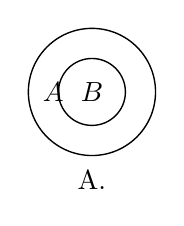
\begin{tikzpicture}[scale=0.85,line width=0.5pt]
\draw (0.9,0.9) circle (0.95);
\draw (0.9,0.9) circle (0.5);
\node at (0.32,0.9) {$A$};
\node at (0.9,0.9) {$B$};
\node[anchor=north] at (0.9,-0.12) {A.};
\end{tikzpicture}
&
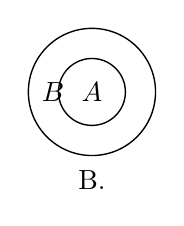
\begin{tikzpicture}[scale=0.85,line width=0.5pt]
\draw (0.9,0.9) circle (0.95);
\draw (0.9,0.9) circle (0.5);
\node at (0.32,0.9) {$B$};
\node at (0.9,0.9) {$A$};
\node[anchor=north] at (0.9,-0.12) {B.};
\end{tikzpicture}
\\[12pt]
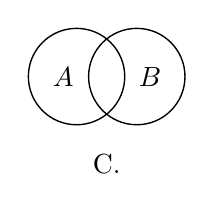
\begin{tikzpicture}[scale=0.85,line width=0.5pt]
\draw (0.65,0.9) circle (0.72);
\draw (1.55,0.9) circle (0.72);
\node at (0.45,0.9) {$A$};
\node at (1.75,0.9) {$B$};
\node[anchor=north] at (1.1,-0.12) {C.};
\end{tikzpicture}
&
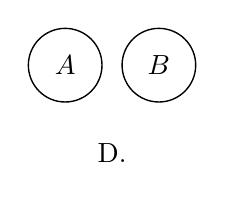
\begin{tikzpicture}[scale=0.85,line width=0.5pt]
\draw (0.55,0.9) circle (0.55);
\draw (1.95,0.9) circle (0.55);
\node at (0.55,0.9) {$A$};
\node at (1.95,0.9) {$B$};
\node[anchor=north] at (1.25,-0.12) {D.};
\end{tikzpicture}
\end{tabular}
\end{center}

\ifanswer
\solbegin
\step{$B\subset A$，图形能表示 $A$ 与 $B$ 关系的是 $A$. 故选 $A$.}
\solend
\fi

\item 以某些整数为元素的集合 $P$ 具有以下性质：

（1）$P$ 中元素有正数，也有负数；（2）$P$ 中元素有奇数，也有偶数；

（3）$-1\notin P$；（4）若 $x$、$y\in P$，则 $x+y\in P$.

则下列选项哪个是正确的\mbox{（\quad）}

\keepwithprev
A. 集合 $P$ 中一定有 $0$ 但没有 $2$\qquad\qquad B. 集合 $P$ 中一定有 $0$ 可能有 $2$

C. 集合 $P$ 中可能有 $0$ 可能有 $2$\qquad\qquad D. 集合 $P$ 中既没有 $0$ 又没有 $2$

\ifanswer
\solbegin
\step{由（4）得 $x\in P$，则 $kx\in P(k$ 是正整数$)$.}
\step{由（1）可设 $x$、$y\in P$，且 $x>0$，$y<0$，则 $xy$、$(-y)x\in P$，}
\step{因而 $0=xy+(-y)x\in P$.}
\step{假设 $2\in P$，则 $2k\in P$. 由上面及（4）得 $0$，$2$，$4$，$6$，$8$，$\cdots$ 均在 $P$ 中，}
\step{故 $2k-2\in P(k$ 是正整数$)$，}
\step{不妨令 $P$ 中负数为奇数 $-2k+1(k$ 为正整数$)$，}
\step{由（4）得 $(2k-2)+(-2k+1)=-1\in P$，矛盾.}
\step{故若 $2\in P$，则 $P$ 中没有负奇数.}
\step{若 $P$ 中负数为偶数，设为 $-2k(k$ 为正整数$)$，则由（4）及 $2\in P$，}
\step{得 $-2$,$-4$,$-6$,$\cdots$ 均在 $P$ 中，即 $-2m-2\in P(m$ 为非负整数$)$，}
\step{则 $P$ 中正奇数为 $2m+1$，由（4）得 $(-2m-2)+(2m+1)=-1\in P$，矛盾.}
\step{综上，$0\in P$，$2\notin P$，故选 $A$.}
\solend
\fi

\end{enumerate}

\bigsec{三、解答题}

\begin{enumerate}
\setcounter{enumi}{16}

\item （1）已知 $a$、$b$ 为实数，比较 $a^2+b^2$ 与 $4a-2b-5$ 的值的大小.

（2）若 $-1\leqslant x+y\leqslant2$，$-2\leqslant x-y\leqslant1$，求 $x-2y$ 的范围.

\ifanswer
\solbegin
\step{（1）$a^2+b^2-(4a-2b-5)=a^2-4a+4+b^2+2b+1=(a-2)^2+(b+1)^2\geqslant0$，}
\step{故 $a^2+b^2\geqslant4a-2b-5$.}
\step{（2）设 $x-2y=m(x+y)+n(x-y)$，则 $x-2y=(m+n)x+(m-n)y$，}
\step{所以 $\begin{cases}m+n=1\\m-n=-2\end{cases}$，解得 $n=\dfrac32$，$m=-\dfrac12$，}
\step{所以 $x-2y=-\dfrac12(x+y)+\dfrac32(x-y)$，}
\step{因为 $-1\leqslant x+y\leqslant2$，$-2\leqslant x-y\leqslant1$，}
\step{所以 $-1\leqslant-\dfrac12(x+y)\leqslant\dfrac12$，$-3\leqslant\dfrac32(x-y)\leqslant\dfrac32$，}
\step{所以 $-4\leqslant-\dfrac12(x+y)+\dfrac32(x-y)\leqslant2$，即 $-4\leqslant x-2y\leqslant2$，}
\step{故 $x-2y$ 的范围是 $[-4,2]$.}
\solend
\fi

\item 已知集合 $A=\{x\mid\lvert x-2\rvert<a\}$，集合 $B=\left\{x\,\middle\vert\,\dfrac{2x-1}{x+2}<1\right\}$.

（1）若 $a=2$，求 $A\cup B$,$A\cap B$；

（2）若 $A\cap B=A$，求实数 $a$ 的取值范围.

\ifanswer
\solbegin
\step{（1）由题意得 $A=(0,4)$,$B=(-2,3)$，所以 $A\cup B=(-2,4)$,$A\cap B=(0,3)$；}
\step{（2）因为 $A\cap B=A$，所以 $A\subseteq B$，}
\step{当 $a\leqslant0$ 时，$A=\varnothing$，满足 $A\subseteq B$；}
\step{当 $a>0$ 时，$A=(2-a,2+a)$,$B=(-2,3)$，}
\step{因为 $A\subseteq B$，所以 $\begin{cases}-2\leqslant2-a\\3\geqslant2+a\end{cases}$，解得 $a\leqslant1$，即 $0<a\leqslant1$.}
\step{因此，实数 $a$ 的取值范围为 $(-\infty,1]$.}
\solend
\fi

\item 我校校园文化节即将到来，高一年级将开展“数字配对”的抽奖活动，活动规则如下：每人可以抽取一张卡片，每张卡片上都印有一个不小于 $-10$ 且不大于 $10$ 的整数，其中不含 $2$. 每张卡片数字对应一个抽奖号码，卡片上的数字减去 $2$ 所得的差，与抽奖号码减去 $3$ 所得的差，两者的乘积等于 $12$.

（1）记卡片上的数字为 $x$，卡片数字对应的抽奖号码为 $y$，请用含有卡片数字 $x$ 的式子来表示抽奖号码 $y$；

（2）当抽奖号码不小于 $3$ 且不大于 $7$ 时，抽奖者可以领取奖品. 请问抽到哪些数字的卡片可以领取奖品？请写出满足领取奖品的卡片数字所组成的集合.

\ifanswer
\solbegin
\step{（1）卡片上的数字为 $x$，对应的抽奖号码为 $y$，}
\step{由题意得 $(x-2)(y-3)=12$，因为 $x\neq2$，所以 $y=3+\dfrac{12}{x-2}$，}
\step{所以 $y=3+\dfrac{12}{x-2}(-10\leqslant x\leqslant10,x\in\Z,x\neq2)$.}
\step{（2）由（1）得 $y=3+\dfrac{12}{x-2}(-10\leqslant x\leqslant10,x\in\Z,x\neq2)$，}
\step{由抽奖条件，得 $3\leqslant3+\dfrac{12}{x-2}\leqslant7$，$x\geqslant5$，所以 $5\leqslant x\leqslant10$，$x\in\Z$，}
\step{所以可领取奖品的卡片数字为 $\{5,6,7,8,9,10\}$.}
\solend
\fi

\item （1）已知 $m\in\R$，若不等式 $(m+1)x^2-mx+m-1<0$ 的解集是空集，求 $m$ 的取值范围；

（2）命题 $P:x^2-5x+6<0$，命题 $q:x^2-4ax+3a^2<0$，若命题 $P$ 是命题 $q$ 的充分非必要条件，求实数 $a$ 的取值范围.

\ifanswer
\solbegin
\step{（1）①当 $m+1=0$，即 $m=-1$ 时，$f(x)=x-2$，不合题意；}
\step{②当 $m+1\neq0$，即 $m\neq-1$ 时，$\begin{cases}m+1>0\\\Delta=m^2-4(m+1)(m-1)\leqslant0\end{cases}$，解得 $m\geqslant\dfrac{2\sqrt3}{3}$，}
\step{所以 $m$ 的取值范围是 $\left[\dfrac{2\sqrt3}{3},+\infty\right)$；}
\step{（2）解 $x^2-5x+6<0$，因式分解得 $(x-2)(x-3)<0$，故 $P$ 的解集为 $(2,3)$，}
\step{解 $x^2-4ax+3a^2<0$，因式分解得 $(x-a)(x-3a)<0$，}
\step{因为命题 $P$ 是命题 $q$ 的充分不必要条件，所以 $(2,3)$ 是 $q$ 解集的真子集，}
\step{当 $a=0$ 时，$q$ 的解集为 $\varnothing$，不合题意，舍去；}
\step{当 $a<0$ 时，$q$ 的解集为 $(3a,a)$，$\begin{cases}3a\leqslant2\\a\geqslant3\end{cases}$，不等式组无解，舍去；}
\step{当 $a>0$ 时，$q$ 的解集为 $(a,3a)$，又因为 $(2,3)$ 是 $q$ 解集的真子集，}
\step{所以 $\begin{cases}a\leqslant2\\3a\geqslant3\end{cases}$（等号不同时取），解得 $1\leqslant a\leqslant2$；}
\step{综上，实数 $a$ 的取值范围是 $[1,2]$.}
\solend
\fi

\item 对于至少含两个元素的有限正整数集 $A$，定义它的“两两和集”为
$S(A)=\{z\mid z=x+y$，其中 $x$、$y\in A$，且 $x<y\}$.

（1）若 $A=\{1,2,4,5\}$，求 $S(A)$；

（2）已知集合 $A$ 中恰好含有四个元素，且 $S(A)=\{5,7,8,10,11,13\}$，写出所有符合条件的集合 $A$；

（3）猜想：当集合 $A$ 含有 $n$ 个元素（$n\geqslant2$）时，$S(A)$ 的元素个数最少是多少？证明你的猜想.

\ifanswer
\solbegin
\step{（1）因为 $A=\{1,2,4,5\}$，计算所有两两和并去掉重复的结果有 $3$，$5$，$6$，$7$，$9$，}
\step{所以 $S(A)=\{3,5,6,7,9\}$.}
\step{（2）设 $A=\{a,b,c,d\}$，其中 $a<b<c<d$，且 $S(A)=\{5,7,8,10,11,13\}$，}
\step{四个元素共有六种两两配对，和集恰好有六个元素，}
\step{因此六个和互不相同.}
\step{这六个数分别为 $a+b$,$a+c$,$a+d$,$b+c$,$b+d$,$c+d$，}
\step{所以这六个数从小到大，可以确定第一个数为 $a+b$，第二数为 $a+c$，}
\step{第五个数为 $b+d$，第六数为 $c+d$，}
\step{第三个数和第四个数不能确定，即 $b+c$ 和 $a+d$ 的大小不定.}
\step{所以 $a+b=5$,$a+c=7$,$b+d=11$,$c+d=13$.}
\step{由此得到 $b=5-a$,$c=7-a$,$d=6+a$，}
\step{于是 $a+d=2a+6$,$b+c=12-2a$.}
\step{其余两个数 $b+c$,$a+d$ 对应 $8$,$10$，分两种情况讨论：}
\step{①若 $b+c=8$,$a+d=10$，则 $\begin{cases}12-2a=8\\2a+6=10\end{cases}$，解得 $a=2$，}
\step{所以 $A=\{2,3,5,8\}$；}
\step{②若 $b+c=10$,$a+d=8$，则 $\begin{cases}12-2a=10\\2a+6=8\end{cases}$，解得 $a=1$，}
\step{所以 $A=\{1,4,6,7\}$；}
\step{检验得，两组均符合题意.}
\step{因此所有符合条件的集合为 $A=\{1,4,6,7\}$ 或 $A=\{2,3,5,8\}$.}
\step{（3）猜想：两两和集的元素个数的最小值为 $2n-3$. 证明如下：}
\step{将集合中的元素按从小到大排列为 $a_1<a_2<\cdots<a_n$，}
\step{当 $n=2$ 时，两两和集恰好有一个元素，结论成立.}
\step{当 $n\geqslant3$ 时，考虑下列均属于 $S(A)$ 的数，}
\step{由不等式的传递性得严格不等式：}
\step{$a_1+a_2<a_1+a_3<\cdots<a_1+a_n<a_2+a_n<\cdots<a_{n-1}+a_n$，}
\step{其中 $a_1+a_2<a_1+a_3<\cdots<a_1+a_n$ 共有 $n-1$ 个不相等的数；}
\step{$a_2+a_n<\cdots<a_{n-1}+a_n$ 共有 $n-2$ 个不相等的数，}
\step{所以一共有 $(n-1)+(n-2)=2n-3$ 个，}
\step{因此，两两和集至少含有 $2n-3$ 个元素.}
\step{再证明可以取到 $2n-3$：}
\step{对任意 $n\geqslant2$，取 $A=\{1,2,\cdots,n\}$，}
\step{所有两两和都是不小于 $3$ 且不大于 $2n-1$ 的整数，}
\step{其中，$1+2$,$1+3$,$\cdots$,$1+n$ 是从 $3$ 到 $n+1$ 的整数；}
\step{当 $n\geqslant3$ 时，$2+n$,$3+n$,$\cdots$,$(n-1)+n$ 可取到其余整数；}
\step{因此 $S(A)=\{3,4,\cdots,2n-1\}$，其元素个数为 $(2n-1)-3+1=2n-3$，}
\step{所以所求最小值为 $2n-3$.}
\solend
\fi

\end{enumerate}

\end{document}
"
% 紧凑版：xelatex "\def\iscompact{1}% 高一118_罗店中学_10月月考.tex
%   —— 高一上数学“2026-2027 年罗店中学高一上 10 月月考”（试卷版/答案版）
% 试卷版：xelatex 高一118_罗店中学_10月月考.tex
% 答案版：xelatex "\def\isanswer{1}% 高一118_罗店中学_10月月考.tex
%   —— 高一上数学“2026-2027 年罗店中学高一上 10 月月考”（试卷版/答案版）
% 试卷版：xelatex 高一118_罗店中学_10月月考.tex
% 答案版：xelatex "\def\isanswer{1}% 高一118_罗店中学_10月月考.tex
%   —— 高一上数学“2026-2027 年罗店中学高一上 10 月月考”（试卷版/答案版）
% 试卷版：xelatex 高一118_罗店中学_10月月考.tex
% 答案版：xelatex "\def\isanswer{1}\input{高一118_罗店中学_10月月考.tex}"
% 紧凑版：xelatex "\def\iscompact{1}\input{高一118_罗店中学_10月月考.tex}"
%
% 原始材料：微信公众号“魔都数学加油站”文章，作者破晓，2026-11-06 17:58 发布；
% 连载“27学年高一118”，原文标题“27学年高一118——2026-2027年上海市罗店中学高一上10月月考”；
% 原文链接：https://mp.weixin.qq.com/s/4edo8awYdjmWJl153X-aDA。
% 正文为 9 张 PNG 页（第 2、3、5、9 页 2560×3620，其余 4762×6735），
% 题目下印有【解析】或【答案】，为讲评版。
% 题目、解析均据原图转录；卷面红色水印及公众号页脚未录入。
%
% 卷首标题：原卷印作“2026-2027 年罗店中学高一上 10 月月考”（公众号标题中的“上海市”
% 卷面标题行没有，本稿照卷面），年份区间按全稿惯例排 en dash；原卷未印副标题，本稿按题目内容
% 标为“集合与常用逻辑用语、不等式”。
%
% 与原卷的排版差异：
%   ① 原文从第 3 题起，填空题 3—12、选择题 13—16、解答题 17—21，共 19 题，本稿保留原题号；
%   ② 原卷每题下直接印【解析】／【答案】，本稿按全稿惯例置于答案版；第 4 题只印【答案】、
%      第 14 题把答案“$B$”印在题干括号内且无【解析】，均另提 \ans{}；其余选择题答案在
%      解析末句“故选 …”，括号内留空；
%   ③ 原卷未印副标题，本稿按“知识模块”口径补出；
%   ④ 原卷填空横线按全稿惯例排为 \blankline[4.4em]；选择题括号排 \mbox{（\quad）}、
%      选项段前按惯例加 \keepwithprev；解答题不留作答区（原卷为讲评版，与 109—117 同）；
%   ⑤ 原卷数集 $R$／$Z$ 按全稿惯例改 \R、\Z，补集照原卷上划线排 \overline{B}。
%
% 子集符号：第 6 题、第 18 题的 $\{x\mid x<1\}\subseteq\{x\mid x<3a-2\}$ 与 $A\subseteq B$
%   印有下划线，照录 \subseteq；第 15 题解析的 $B\subset A$ 印单线（真子集、无下划线），
%   按 18／96 成例照录 \subset。
%
% 判别式字形：第 20 题 (1) cases 的判别式原卷排 $\Delta$（等腰、右厚），照录 \Delta。
%
% 图与表：第 9 题题干的文氏图（矩形 $U$ 内两椭圆 $A$、$B$，阴影为 $A\cap\overline B$）
%   按原图形状用 TikZ 重绘（三版都出）；第 12 题解析的“列表”按原卷用 tabular 重排
%   （仅答案版）；第 15 题四个文氏图选项按原图形状用 TikZ 重排（三版都出）。
%
% 原卷存疑照录：第 8 题解析“$2022+3\cdot1\cdot(-1)=2026$”一行、第 11 题解析结论
%   作“必要不充分条件”而选项列“必要非充分”、第 20 题 (2) 的 cases，均照录加注。
%
% 行数核对：逐题数 \step/\stepm 条数，合计 110 条（Q3：2；Q4：0；Q5：1；Q6：2；Q7：5；
% Q8：3；Q9：2；Q10：4；Q11：4；Q12：2；Q13：3；Q14：0；Q15：1；Q16：12；Q17：9；
% Q18：6；Q19：6；Q20：11；Q21：36），与原卷印刷行逐题相等（cases／tabular／TikZ
% 图块作一个印刷行计）。第 4 题只印【答案】、第 14 题括号内印答案且无解析，均提 \ans{}，
% 不计入 \step 账。
%
\documentclass[a4paper,11pt]{article}
\usepackage{common}

\begin{document}

\examtitlest[3]{2026--2027 年罗店中学高一上 10 月月考}{集合与常用逻辑用语、不等式}

\bigsec{一、填空题}

\begin{enumerate}
\setcounter{enumi}{2}

\item 若 $2x^2+3x+5=a(2x+1)(x+1)+b$ 恒成立，则 $a-b$ 的值\blankline[4.4em].

\ifanswer
\solbegin
\step{因为 $2x^2+3x+5=a(2x+1)(x+1)+b=2ax^2+3ax+a+b$ 恒成立，}
\step{所以 $\begin{cases}2=2a\\3=3a\\5=a+b\end{cases}$，所以 $\begin{cases}a=1\\b=4\end{cases}$，故 $a-b$ 的值为 $-3$.}
\solend
\fi

\item “$a$、$b$ 中至少有一个能被 $6$ 整除”的否定形式是\blankline[4.4em].

\ifanswer
\ans{$a$、$b$ 都不能被 $6$ 整除}
\fi

\item 设集合 $A=\{1,2\}$，则满足 $A\cup B=\{1,2,3\}$ 的集合 $B$ 的个数是\blankline[4.4em].

\ifanswer
\solbegin
\step{$B=\{3\}$,$\{1,3\}$,$\{2,3\}$,$\{1,2,3\}$，个数为 $4$.}
\solend
\fi

\item 命题“若 $x<1$，则 $x<3a-2$”是真命题，求实数 $a$ 的取值范围是\blankline[4.4em].

\ifanswer
\solbegin
\step{$\alpha:x<1$,$\beta:x<3a-2$，且若 $\alpha$ 则 $\beta$ 是真命题，}
\step{则 $\{x\mid x<1\}\subseteq\{x\mid x<3a-2\}$，所以 $3a-2\geqslant1$，解得 $a\geqslant1$.}
\solend
\fi

\item 不论实数 $m$ 取什么值，点 $P(m+1,2-m)$ 一定不在第\blankline[4.4em]象限（选填“一”、“二”、“三”或“四”）.

\ifanswer
\solbegin
\step{当 $m+1>0$，$2-m>0$ 时，解得 $-1<m<2$，此时点 $P$ 在第一象限；}
\step{当 $m+1<0$，$2-m>0$ 时，解得 $m<-1$，此时点 $P$ 在第二象限；}
\step{当 $m+1<0$，$2-m<0$ 时，$m$ 无解，此时点 $P$ 不可能在第三象限；}
\step{当 $m+1>0$，$2-m<0$ 时，解得 $m>2$，此时点 $P$ 在第四象限.}
\step{故一定不在第三象限.}
\solend
\fi

\item 设 $x_1$、$x_2$ 是方程 $x^2+x-3=0$ 的两个实数根，则 $x_1^2-x_2+2022=$\blankline[4.4em].

\ifanswer
\solbegin
\step{$x_1$、$x_2$ 是方程 $x^2+x-3=0$ 的两个实数根，}
\step{得 $x_1+x_2=-1$，$x_1^2+x_1-3=0$，所以 $x_1^2=3-x_1$，}
\step{$x_1^2-x_2+2022=3-x_1-x_2+2022=2022+3\cdot1\cdot(-1)=2026$.}
\solend
\fi

\item 如图，已知全集 $U=\R$，集合 $A=\{x\mid y=\sqrt{-x^2+x+2}\}$，$B=\{x\mid x<0$ 或 $x>5\}$. 集合 $C$ 表示图中阴影区域对应的集合，则集合 $C=$\blankline[4.4em]（用区间表示）.

\begin{center}
% 原卷文氏图：矩形 U 内两椭圆 A（阴影）、B，阴影为 A\cap\overline B，按原图形状用 TikZ 重绘。
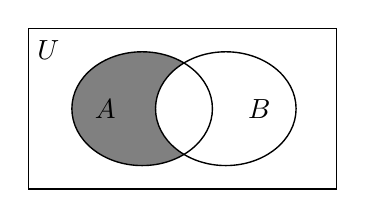
\begin{tikzpicture}[scale=0.85,line width=0.5pt]
\draw (0,0) rectangle (4.6,2.4);
\fill[gray] (1.7,1.2) ellipse (1.05 and 0.85);
\fill[white] (2.95,1.2) ellipse (1.05 and 0.85);
\draw (1.7,1.2) ellipse (1.05 and 0.85);
\draw (2.95,1.2) ellipse (1.05 and 0.85);
\node at (1.15,1.2) {$A$};
\node at (3.45,1.2) {$B$};
\node at (0.3,2.08) {$U$};
\end{tikzpicture}
\end{center}

\ifanswer
\solbegin
\step{$A=\{x\mid y=\sqrt{-x^2+x+2}\}=\{x\mid-1\leqslant x\leqslant2\}$，}
\step{$\overline B=\{x\mid 0\leqslant x\leqslant5\}$，$C=A\cap\overline B=[0,2]$.}
\solend
\fi

\item 关于 $x$ 的不等式 $ax-b<0$ 的解集为 $(2,+\infty)$，则关于 $x$ 的不等式 $(ax+b)(x-1)<0$ 的解集为\blankline[4.4em].

\ifanswer
\solbegin
\step{因为关于 $x$ 的不等式 $ax-b<0$ 的解集为 $(2,+\infty)$，所以 $\begin{cases}a<0\\2a-b=0\end{cases}$，}
\step{所以不等式 $(ax+b)(x-1)<0$ 可化为 $a\left(x+\dfrac ba\right)(x-1)<0$，$a<0$，}
\step{所以 $(x+2)(x-1)>0$，}
\step{所以所求解集为 $(-\infty,-2)\cup(1,+\infty)$.}
\solend
\fi

\item $a_1$、$b_1$、$a_2$、$b_2$ 均为非零实数，不等式 $a_1x+b_1>0$ 和 $a_2x+b_2>0$ 的解集分别为集合 $M$、$N$，那么“$\dfrac{a_1}{a_2}=\dfrac{b_1}{b_2}$”是“$M=N$”的\blankline[4.4em]条件（选填“充分非必要”、“必要非充分”、“充要”和“既非充分也非必要”）.

\ifanswer
\solbegin
\step{当 $a_1=b_1=1$，$a_2=b_2=-1$ 时，满足 $\dfrac{a_1}{a_2}=\dfrac{b_1}{b_2}$，}
\step{但是 $M=N$ 不成立，即充分性不成立；}
\step{若 $M=N$ 时，$\dfrac{a_1}{a_2}=\dfrac{b_1}{b_2}$ 一定成立，即必要性成立.}
\step{故为必要不充分条件.}% 原卷选项列“必要非充分”、解析结论作“必要不充分”，照录
\solend
\fi

\item 已知集合 $\{a,b,c\}=\{0,1,2\}$，且下列三个关系：① $a\neq2$；② $b=2$；③ $c\neq0$；有且只有一个正确，则 $100a+10b+c=$\blankline[4.4em].

\ifanswer
\solbegin
\step{列表如下：}
\begin{center}
\begin{tabular}{|c|c|c|c|c|}
\hline
 & ① & ② & ③ & \\
\hline
① 正确 & $a\neq2$ & $b\neq2$ & $c=0$ & 无解\\
\hline
② 正确 & $a=2$ & $b=2$ & $c=0$ & 矛盾\\
\hline
③ 正确 & $a=2$ & $b\neq2$ & $c\neq0$ & $a=2,b=0,c=1$\\
\hline
\end{tabular}
\end{center}
\step{所以 $100a+10b+c=201$.}
\solend
\fi

\end{enumerate}

\bigsec{二、选择题}

\begin{enumerate}
\setcounter{enumi}{12}

\item 已知 $a$,$b$,$c\in\R$,$b>c$，则下列不等式中恒成立的是\mbox{（\quad）}

\keepwithprev
A. $a+b^2>a+c^2$\qquad\quad B. $a^2+b>a^2+c$\qquad\quad C. $ab^2>ac^2$\qquad\quad D. $a^2b>a^2c$

\ifanswer
\solbegin
\step{对于 $A$，取 $b=1,c=-1$，错误；对于 $B$，由不等式的同向可加性得正确；}
\step{对于 $C$，取 $a=1,b=1,c=-2$，错误；对于 $D$，取 $a=0$，错误；}
\step{故选 $B$.}
\solend
\fi

\item 给出命题：“如果 $n$ 是素数，那么 $n^2+2$ 不是素数”，甲同学判断该命题是假命题，他做出这个判断的反例可以是\mbox{（\quad）}% 原卷把答案“$B$”印在题干括号内、无【解析】

\keepwithprev
A. $n=2$\qquad\quad B. $n=3$\qquad\quad C. $n=4$\qquad\quad D. $n=5$

\ifanswer
\ans{$B$}
\fi

\item 设集合 $A=\left\{x\,\middle\vert\,x=\dfrac n2,n\in\Z\right\}$，$B=\left\{x\,\middle\vert\,x=n+\dfrac12,n\in\Z\right\}$，则下列图形能表示 $A$ 与 $B$ 关系的是\mbox{（\quad）}

\keepwithprev
\begin{center}
% 原卷四个文氏图选项按原图形状用 TikZ 重排。
\begin{tabular}{c@{\qquad\qquad}c}
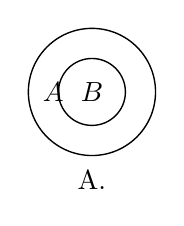
\begin{tikzpicture}[scale=0.85,line width=0.5pt]
\draw (0.9,0.9) circle (0.95);
\draw (0.9,0.9) circle (0.5);
\node at (0.32,0.9) {$A$};
\node at (0.9,0.9) {$B$};
\node[anchor=north] at (0.9,-0.12) {A.};
\end{tikzpicture}
&
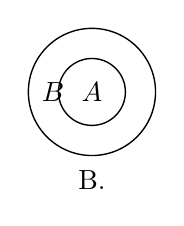
\begin{tikzpicture}[scale=0.85,line width=0.5pt]
\draw (0.9,0.9) circle (0.95);
\draw (0.9,0.9) circle (0.5);
\node at (0.32,0.9) {$B$};
\node at (0.9,0.9) {$A$};
\node[anchor=north] at (0.9,-0.12) {B.};
\end{tikzpicture}
\\[12pt]
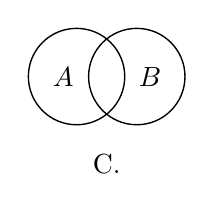
\begin{tikzpicture}[scale=0.85,line width=0.5pt]
\draw (0.65,0.9) circle (0.72);
\draw (1.55,0.9) circle (0.72);
\node at (0.45,0.9) {$A$};
\node at (1.75,0.9) {$B$};
\node[anchor=north] at (1.1,-0.12) {C.};
\end{tikzpicture}
&
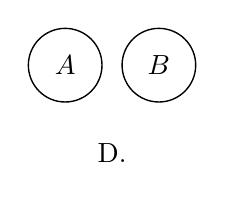
\begin{tikzpicture}[scale=0.85,line width=0.5pt]
\draw (0.55,0.9) circle (0.55);
\draw (1.95,0.9) circle (0.55);
\node at (0.55,0.9) {$A$};
\node at (1.95,0.9) {$B$};
\node[anchor=north] at (1.25,-0.12) {D.};
\end{tikzpicture}
\end{tabular}
\end{center}

\ifanswer
\solbegin
\step{$B\subset A$，图形能表示 $A$ 与 $B$ 关系的是 $A$. 故选 $A$.}
\solend
\fi

\item 以某些整数为元素的集合 $P$ 具有以下性质：

（1）$P$ 中元素有正数，也有负数；（2）$P$ 中元素有奇数，也有偶数；

（3）$-1\notin P$；（4）若 $x$、$y\in P$，则 $x+y\in P$.

则下列选项哪个是正确的\mbox{（\quad）}

\keepwithprev
A. 集合 $P$ 中一定有 $0$ 但没有 $2$\qquad\qquad B. 集合 $P$ 中一定有 $0$ 可能有 $2$

C. 集合 $P$ 中可能有 $0$ 可能有 $2$\qquad\qquad D. 集合 $P$ 中既没有 $0$ 又没有 $2$

\ifanswer
\solbegin
\step{由（4）得 $x\in P$，则 $kx\in P(k$ 是正整数$)$.}
\step{由（1）可设 $x$、$y\in P$，且 $x>0$，$y<0$，则 $xy$、$(-y)x\in P$，}
\step{因而 $0=xy+(-y)x\in P$.}
\step{假设 $2\in P$，则 $2k\in P$. 由上面及（4）得 $0$，$2$，$4$，$6$，$8$，$\cdots$ 均在 $P$ 中，}
\step{故 $2k-2\in P(k$ 是正整数$)$，}
\step{不妨令 $P$ 中负数为奇数 $-2k+1(k$ 为正整数$)$，}
\step{由（4）得 $(2k-2)+(-2k+1)=-1\in P$，矛盾.}
\step{故若 $2\in P$，则 $P$ 中没有负奇数.}
\step{若 $P$ 中负数为偶数，设为 $-2k(k$ 为正整数$)$，则由（4）及 $2\in P$，}
\step{得 $-2$,$-4$,$-6$,$\cdots$ 均在 $P$ 中，即 $-2m-2\in P(m$ 为非负整数$)$，}
\step{则 $P$ 中正奇数为 $2m+1$，由（4）得 $(-2m-2)+(2m+1)=-1\in P$，矛盾.}
\step{综上，$0\in P$，$2\notin P$，故选 $A$.}
\solend
\fi

\end{enumerate}

\bigsec{三、解答题}

\begin{enumerate}
\setcounter{enumi}{16}

\item （1）已知 $a$、$b$ 为实数，比较 $a^2+b^2$ 与 $4a-2b-5$ 的值的大小.

（2）若 $-1\leqslant x+y\leqslant2$，$-2\leqslant x-y\leqslant1$，求 $x-2y$ 的范围.

\ifanswer
\solbegin
\step{（1）$a^2+b^2-(4a-2b-5)=a^2-4a+4+b^2+2b+1=(a-2)^2+(b+1)^2\geqslant0$，}
\step{故 $a^2+b^2\geqslant4a-2b-5$.}
\step{（2）设 $x-2y=m(x+y)+n(x-y)$，则 $x-2y=(m+n)x+(m-n)y$，}
\step{所以 $\begin{cases}m+n=1\\m-n=-2\end{cases}$，解得 $n=\dfrac32$，$m=-\dfrac12$，}
\step{所以 $x-2y=-\dfrac12(x+y)+\dfrac32(x-y)$，}
\step{因为 $-1\leqslant x+y\leqslant2$，$-2\leqslant x-y\leqslant1$，}
\step{所以 $-1\leqslant-\dfrac12(x+y)\leqslant\dfrac12$，$-3\leqslant\dfrac32(x-y)\leqslant\dfrac32$，}
\step{所以 $-4\leqslant-\dfrac12(x+y)+\dfrac32(x-y)\leqslant2$，即 $-4\leqslant x-2y\leqslant2$，}
\step{故 $x-2y$ 的范围是 $[-4,2]$.}
\solend
\fi

\item 已知集合 $A=\{x\mid\lvert x-2\rvert<a\}$，集合 $B=\left\{x\,\middle\vert\,\dfrac{2x-1}{x+2}<1\right\}$.

（1）若 $a=2$，求 $A\cup B$,$A\cap B$；

（2）若 $A\cap B=A$，求实数 $a$ 的取值范围.

\ifanswer
\solbegin
\step{（1）由题意得 $A=(0,4)$,$B=(-2,3)$，所以 $A\cup B=(-2,4)$,$A\cap B=(0,3)$；}
\step{（2）因为 $A\cap B=A$，所以 $A\subseteq B$，}
\step{当 $a\leqslant0$ 时，$A=\varnothing$，满足 $A\subseteq B$；}
\step{当 $a>0$ 时，$A=(2-a,2+a)$,$B=(-2,3)$，}
\step{因为 $A\subseteq B$，所以 $\begin{cases}-2\leqslant2-a\\3\geqslant2+a\end{cases}$，解得 $a\leqslant1$，即 $0<a\leqslant1$.}
\step{因此，实数 $a$ 的取值范围为 $(-\infty,1]$.}
\solend
\fi

\item 我校校园文化节即将到来，高一年级将开展“数字配对”的抽奖活动，活动规则如下：每人可以抽取一张卡片，每张卡片上都印有一个不小于 $-10$ 且不大于 $10$ 的整数，其中不含 $2$. 每张卡片数字对应一个抽奖号码，卡片上的数字减去 $2$ 所得的差，与抽奖号码减去 $3$ 所得的差，两者的乘积等于 $12$.

（1）记卡片上的数字为 $x$，卡片数字对应的抽奖号码为 $y$，请用含有卡片数字 $x$ 的式子来表示抽奖号码 $y$；

（2）当抽奖号码不小于 $3$ 且不大于 $7$ 时，抽奖者可以领取奖品. 请问抽到哪些数字的卡片可以领取奖品？请写出满足领取奖品的卡片数字所组成的集合.

\ifanswer
\solbegin
\step{（1）卡片上的数字为 $x$，对应的抽奖号码为 $y$，}
\step{由题意得 $(x-2)(y-3)=12$，因为 $x\neq2$，所以 $y=3+\dfrac{12}{x-2}$，}
\step{所以 $y=3+\dfrac{12}{x-2}(-10\leqslant x\leqslant10,x\in\Z,x\neq2)$.}
\step{（2）由（1）得 $y=3+\dfrac{12}{x-2}(-10\leqslant x\leqslant10,x\in\Z,x\neq2)$，}
\step{由抽奖条件，得 $3\leqslant3+\dfrac{12}{x-2}\leqslant7$，$x\geqslant5$，所以 $5\leqslant x\leqslant10$，$x\in\Z$，}
\step{所以可领取奖品的卡片数字为 $\{5,6,7,8,9,10\}$.}
\solend
\fi

\item （1）已知 $m\in\R$，若不等式 $(m+1)x^2-mx+m-1<0$ 的解集是空集，求 $m$ 的取值范围；

（2）命题 $P:x^2-5x+6<0$，命题 $q:x^2-4ax+3a^2<0$，若命题 $P$ 是命题 $q$ 的充分非必要条件，求实数 $a$ 的取值范围.

\ifanswer
\solbegin
\step{（1）①当 $m+1=0$，即 $m=-1$ 时，$f(x)=x-2$，不合题意；}
\step{②当 $m+1\neq0$，即 $m\neq-1$ 时，$\begin{cases}m+1>0\\\Delta=m^2-4(m+1)(m-1)\leqslant0\end{cases}$，解得 $m\geqslant\dfrac{2\sqrt3}{3}$，}
\step{所以 $m$ 的取值范围是 $\left[\dfrac{2\sqrt3}{3},+\infty\right)$；}
\step{（2）解 $x^2-5x+6<0$，因式分解得 $(x-2)(x-3)<0$，故 $P$ 的解集为 $(2,3)$，}
\step{解 $x^2-4ax+3a^2<0$，因式分解得 $(x-a)(x-3a)<0$，}
\step{因为命题 $P$ 是命题 $q$ 的充分不必要条件，所以 $(2,3)$ 是 $q$ 解集的真子集，}
\step{当 $a=0$ 时，$q$ 的解集为 $\varnothing$，不合题意，舍去；}
\step{当 $a<0$ 时，$q$ 的解集为 $(3a,a)$，$\begin{cases}3a\leqslant2\\a\geqslant3\end{cases}$，不等式组无解，舍去；}
\step{当 $a>0$ 时，$q$ 的解集为 $(a,3a)$，又因为 $(2,3)$ 是 $q$ 解集的真子集，}
\step{所以 $\begin{cases}a\leqslant2\\3a\geqslant3\end{cases}$（等号不同时取），解得 $1\leqslant a\leqslant2$；}
\step{综上，实数 $a$ 的取值范围是 $[1,2]$.}
\solend
\fi

\item 对于至少含两个元素的有限正整数集 $A$，定义它的“两两和集”为
$S(A)=\{z\mid z=x+y$，其中 $x$、$y\in A$，且 $x<y\}$.

（1）若 $A=\{1,2,4,5\}$，求 $S(A)$；

（2）已知集合 $A$ 中恰好含有四个元素，且 $S(A)=\{5,7,8,10,11,13\}$，写出所有符合条件的集合 $A$；

（3）猜想：当集合 $A$ 含有 $n$ 个元素（$n\geqslant2$）时，$S(A)$ 的元素个数最少是多少？证明你的猜想.

\ifanswer
\solbegin
\step{（1）因为 $A=\{1,2,4,5\}$，计算所有两两和并去掉重复的结果有 $3$，$5$，$6$，$7$，$9$，}
\step{所以 $S(A)=\{3,5,6,7,9\}$.}
\step{（2）设 $A=\{a,b,c,d\}$，其中 $a<b<c<d$，且 $S(A)=\{5,7,8,10,11,13\}$，}
\step{四个元素共有六种两两配对，和集恰好有六个元素，}
\step{因此六个和互不相同.}
\step{这六个数分别为 $a+b$,$a+c$,$a+d$,$b+c$,$b+d$,$c+d$，}
\step{所以这六个数从小到大，可以确定第一个数为 $a+b$，第二数为 $a+c$，}
\step{第五个数为 $b+d$，第六数为 $c+d$，}
\step{第三个数和第四个数不能确定，即 $b+c$ 和 $a+d$ 的大小不定.}
\step{所以 $a+b=5$,$a+c=7$,$b+d=11$,$c+d=13$.}
\step{由此得到 $b=5-a$,$c=7-a$,$d=6+a$，}
\step{于是 $a+d=2a+6$,$b+c=12-2a$.}
\step{其余两个数 $b+c$,$a+d$ 对应 $8$,$10$，分两种情况讨论：}
\step{①若 $b+c=8$,$a+d=10$，则 $\begin{cases}12-2a=8\\2a+6=10\end{cases}$，解得 $a=2$，}
\step{所以 $A=\{2,3,5,8\}$；}
\step{②若 $b+c=10$,$a+d=8$，则 $\begin{cases}12-2a=10\\2a+6=8\end{cases}$，解得 $a=1$，}
\step{所以 $A=\{1,4,6,7\}$；}
\step{检验得，两组均符合题意.}
\step{因此所有符合条件的集合为 $A=\{1,4,6,7\}$ 或 $A=\{2,3,5,8\}$.}
\step{（3）猜想：两两和集的元素个数的最小值为 $2n-3$. 证明如下：}
\step{将集合中的元素按从小到大排列为 $a_1<a_2<\cdots<a_n$，}
\step{当 $n=2$ 时，两两和集恰好有一个元素，结论成立.}
\step{当 $n\geqslant3$ 时，考虑下列均属于 $S(A)$ 的数，}
\step{由不等式的传递性得严格不等式：}
\step{$a_1+a_2<a_1+a_3<\cdots<a_1+a_n<a_2+a_n<\cdots<a_{n-1}+a_n$，}
\step{其中 $a_1+a_2<a_1+a_3<\cdots<a_1+a_n$ 共有 $n-1$ 个不相等的数；}
\step{$a_2+a_n<\cdots<a_{n-1}+a_n$ 共有 $n-2$ 个不相等的数，}
\step{所以一共有 $(n-1)+(n-2)=2n-3$ 个，}
\step{因此，两两和集至少含有 $2n-3$ 个元素.}
\step{再证明可以取到 $2n-3$：}
\step{对任意 $n\geqslant2$，取 $A=\{1,2,\cdots,n\}$，}
\step{所有两两和都是不小于 $3$ 且不大于 $2n-1$ 的整数，}
\step{其中，$1+2$,$1+3$,$\cdots$,$1+n$ 是从 $3$ 到 $n+1$ 的整数；}
\step{当 $n\geqslant3$ 时，$2+n$,$3+n$,$\cdots$,$(n-1)+n$ 可取到其余整数；}
\step{因此 $S(A)=\{3,4,\cdots,2n-1\}$，其元素个数为 $(2n-1)-3+1=2n-3$，}
\step{所以所求最小值为 $2n-3$.}
\solend
\fi

\end{enumerate}

\end{document}
"
% 紧凑版：xelatex "\def\iscompact{1}% 高一118_罗店中学_10月月考.tex
%   —— 高一上数学“2026-2027 年罗店中学高一上 10 月月考”（试卷版/答案版）
% 试卷版：xelatex 高一118_罗店中学_10月月考.tex
% 答案版：xelatex "\def\isanswer{1}\input{高一118_罗店中学_10月月考.tex}"
% 紧凑版：xelatex "\def\iscompact{1}\input{高一118_罗店中学_10月月考.tex}"
%
% 原始材料：微信公众号“魔都数学加油站”文章，作者破晓，2026-11-06 17:58 发布；
% 连载“27学年高一118”，原文标题“27学年高一118——2026-2027年上海市罗店中学高一上10月月考”；
% 原文链接：https://mp.weixin.qq.com/s/4edo8awYdjmWJl153X-aDA。
% 正文为 9 张 PNG 页（第 2、3、5、9 页 2560×3620，其余 4762×6735），
% 题目下印有【解析】或【答案】，为讲评版。
% 题目、解析均据原图转录；卷面红色水印及公众号页脚未录入。
%
% 卷首标题：原卷印作“2026-2027 年罗店中学高一上 10 月月考”（公众号标题中的“上海市”
% 卷面标题行没有，本稿照卷面），年份区间按全稿惯例排 en dash；原卷未印副标题，本稿按题目内容
% 标为“集合与常用逻辑用语、不等式”。
%
% 与原卷的排版差异：
%   ① 原文从第 3 题起，填空题 3—12、选择题 13—16、解答题 17—21，共 19 题，本稿保留原题号；
%   ② 原卷每题下直接印【解析】／【答案】，本稿按全稿惯例置于答案版；第 4 题只印【答案】、
%      第 14 题把答案“$B$”印在题干括号内且无【解析】，均另提 \ans{}；其余选择题答案在
%      解析末句“故选 …”，括号内留空；
%   ③ 原卷未印副标题，本稿按“知识模块”口径补出；
%   ④ 原卷填空横线按全稿惯例排为 \blankline[4.4em]；选择题括号排 \mbox{（\quad）}、
%      选项段前按惯例加 \keepwithprev；解答题不留作答区（原卷为讲评版，与 109—117 同）；
%   ⑤ 原卷数集 $R$／$Z$ 按全稿惯例改 \R、\Z，补集照原卷上划线排 \overline{B}。
%
% 子集符号：第 6 题、第 18 题的 $\{x\mid x<1\}\subseteq\{x\mid x<3a-2\}$ 与 $A\subseteq B$
%   印有下划线，照录 \subseteq；第 15 题解析的 $B\subset A$ 印单线（真子集、无下划线），
%   按 18／96 成例照录 \subset。
%
% 判别式字形：第 20 题 (1) cases 的判别式原卷排 $\Delta$（等腰、右厚），照录 \Delta。
%
% 图与表：第 9 题题干的文氏图（矩形 $U$ 内两椭圆 $A$、$B$，阴影为 $A\cap\overline B$）
%   按原图形状用 TikZ 重绘（三版都出）；第 12 题解析的“列表”按原卷用 tabular 重排
%   （仅答案版）；第 15 题四个文氏图选项按原图形状用 TikZ 重排（三版都出）。
%
% 原卷存疑照录：第 8 题解析“$2022+3\cdot1\cdot(-1)=2026$”一行、第 11 题解析结论
%   作“必要不充分条件”而选项列“必要非充分”、第 20 题 (2) 的 cases，均照录加注。
%
% 行数核对：逐题数 \step/\stepm 条数，合计 110 条（Q3：2；Q4：0；Q5：1；Q6：2；Q7：5；
% Q8：3；Q9：2；Q10：4；Q11：4；Q12：2；Q13：3；Q14：0；Q15：1；Q16：12；Q17：9；
% Q18：6；Q19：6；Q20：11；Q21：36），与原卷印刷行逐题相等（cases／tabular／TikZ
% 图块作一个印刷行计）。第 4 题只印【答案】、第 14 题括号内印答案且无解析，均提 \ans{}，
% 不计入 \step 账。
%
\documentclass[a4paper,11pt]{article}
\usepackage{common}

\begin{document}

\examtitlest[3]{2026--2027 年罗店中学高一上 10 月月考}{集合与常用逻辑用语、不等式}

\bigsec{一、填空题}

\begin{enumerate}
\setcounter{enumi}{2}

\item 若 $2x^2+3x+5=a(2x+1)(x+1)+b$ 恒成立，则 $a-b$ 的值\blankline[4.4em].

\ifanswer
\solbegin
\step{因为 $2x^2+3x+5=a(2x+1)(x+1)+b=2ax^2+3ax+a+b$ 恒成立，}
\step{所以 $\begin{cases}2=2a\\3=3a\\5=a+b\end{cases}$，所以 $\begin{cases}a=1\\b=4\end{cases}$，故 $a-b$ 的值为 $-3$.}
\solend
\fi

\item “$a$、$b$ 中至少有一个能被 $6$ 整除”的否定形式是\blankline[4.4em].

\ifanswer
\ans{$a$、$b$ 都不能被 $6$ 整除}
\fi

\item 设集合 $A=\{1,2\}$，则满足 $A\cup B=\{1,2,3\}$ 的集合 $B$ 的个数是\blankline[4.4em].

\ifanswer
\solbegin
\step{$B=\{3\}$,$\{1,3\}$,$\{2,3\}$,$\{1,2,3\}$，个数为 $4$.}
\solend
\fi

\item 命题“若 $x<1$，则 $x<3a-2$”是真命题，求实数 $a$ 的取值范围是\blankline[4.4em].

\ifanswer
\solbegin
\step{$\alpha:x<1$,$\beta:x<3a-2$，且若 $\alpha$ 则 $\beta$ 是真命题，}
\step{则 $\{x\mid x<1\}\subseteq\{x\mid x<3a-2\}$，所以 $3a-2\geqslant1$，解得 $a\geqslant1$.}
\solend
\fi

\item 不论实数 $m$ 取什么值，点 $P(m+1,2-m)$ 一定不在第\blankline[4.4em]象限（选填“一”、“二”、“三”或“四”）.

\ifanswer
\solbegin
\step{当 $m+1>0$，$2-m>0$ 时，解得 $-1<m<2$，此时点 $P$ 在第一象限；}
\step{当 $m+1<0$，$2-m>0$ 时，解得 $m<-1$，此时点 $P$ 在第二象限；}
\step{当 $m+1<0$，$2-m<0$ 时，$m$ 无解，此时点 $P$ 不可能在第三象限；}
\step{当 $m+1>0$，$2-m<0$ 时，解得 $m>2$，此时点 $P$ 在第四象限.}
\step{故一定不在第三象限.}
\solend
\fi

\item 设 $x_1$、$x_2$ 是方程 $x^2+x-3=0$ 的两个实数根，则 $x_1^2-x_2+2022=$\blankline[4.4em].

\ifanswer
\solbegin
\step{$x_1$、$x_2$ 是方程 $x^2+x-3=0$ 的两个实数根，}
\step{得 $x_1+x_2=-1$，$x_1^2+x_1-3=0$，所以 $x_1^2=3-x_1$，}
\step{$x_1^2-x_2+2022=3-x_1-x_2+2022=2022+3\cdot1\cdot(-1)=2026$.}
\solend
\fi

\item 如图，已知全集 $U=\R$，集合 $A=\{x\mid y=\sqrt{-x^2+x+2}\}$，$B=\{x\mid x<0$ 或 $x>5\}$. 集合 $C$ 表示图中阴影区域对应的集合，则集合 $C=$\blankline[4.4em]（用区间表示）.

\begin{center}
% 原卷文氏图：矩形 U 内两椭圆 A（阴影）、B，阴影为 A\cap\overline B，按原图形状用 TikZ 重绘。
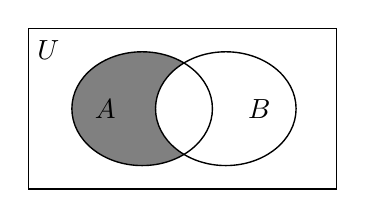
\begin{tikzpicture}[scale=0.85,line width=0.5pt]
\draw (0,0) rectangle (4.6,2.4);
\fill[gray] (1.7,1.2) ellipse (1.05 and 0.85);
\fill[white] (2.95,1.2) ellipse (1.05 and 0.85);
\draw (1.7,1.2) ellipse (1.05 and 0.85);
\draw (2.95,1.2) ellipse (1.05 and 0.85);
\node at (1.15,1.2) {$A$};
\node at (3.45,1.2) {$B$};
\node at (0.3,2.08) {$U$};
\end{tikzpicture}
\end{center}

\ifanswer
\solbegin
\step{$A=\{x\mid y=\sqrt{-x^2+x+2}\}=\{x\mid-1\leqslant x\leqslant2\}$，}
\step{$\overline B=\{x\mid 0\leqslant x\leqslant5\}$，$C=A\cap\overline B=[0,2]$.}
\solend
\fi

\item 关于 $x$ 的不等式 $ax-b<0$ 的解集为 $(2,+\infty)$，则关于 $x$ 的不等式 $(ax+b)(x-1)<0$ 的解集为\blankline[4.4em].

\ifanswer
\solbegin
\step{因为关于 $x$ 的不等式 $ax-b<0$ 的解集为 $(2,+\infty)$，所以 $\begin{cases}a<0\\2a-b=0\end{cases}$，}
\step{所以不等式 $(ax+b)(x-1)<0$ 可化为 $a\left(x+\dfrac ba\right)(x-1)<0$，$a<0$，}
\step{所以 $(x+2)(x-1)>0$，}
\step{所以所求解集为 $(-\infty,-2)\cup(1,+\infty)$.}
\solend
\fi

\item $a_1$、$b_1$、$a_2$、$b_2$ 均为非零实数，不等式 $a_1x+b_1>0$ 和 $a_2x+b_2>0$ 的解集分别为集合 $M$、$N$，那么“$\dfrac{a_1}{a_2}=\dfrac{b_1}{b_2}$”是“$M=N$”的\blankline[4.4em]条件（选填“充分非必要”、“必要非充分”、“充要”和“既非充分也非必要”）.

\ifanswer
\solbegin
\step{当 $a_1=b_1=1$，$a_2=b_2=-1$ 时，满足 $\dfrac{a_1}{a_2}=\dfrac{b_1}{b_2}$，}
\step{但是 $M=N$ 不成立，即充分性不成立；}
\step{若 $M=N$ 时，$\dfrac{a_1}{a_2}=\dfrac{b_1}{b_2}$ 一定成立，即必要性成立.}
\step{故为必要不充分条件.}% 原卷选项列“必要非充分”、解析结论作“必要不充分”，照录
\solend
\fi

\item 已知集合 $\{a,b,c\}=\{0,1,2\}$，且下列三个关系：① $a\neq2$；② $b=2$；③ $c\neq0$；有且只有一个正确，则 $100a+10b+c=$\blankline[4.4em].

\ifanswer
\solbegin
\step{列表如下：}
\begin{center}
\begin{tabular}{|c|c|c|c|c|}
\hline
 & ① & ② & ③ & \\
\hline
① 正确 & $a\neq2$ & $b\neq2$ & $c=0$ & 无解\\
\hline
② 正确 & $a=2$ & $b=2$ & $c=0$ & 矛盾\\
\hline
③ 正确 & $a=2$ & $b\neq2$ & $c\neq0$ & $a=2,b=0,c=1$\\
\hline
\end{tabular}
\end{center}
\step{所以 $100a+10b+c=201$.}
\solend
\fi

\end{enumerate}

\bigsec{二、选择题}

\begin{enumerate}
\setcounter{enumi}{12}

\item 已知 $a$,$b$,$c\in\R$,$b>c$，则下列不等式中恒成立的是\mbox{（\quad）}

\keepwithprev
A. $a+b^2>a+c^2$\qquad\quad B. $a^2+b>a^2+c$\qquad\quad C. $ab^2>ac^2$\qquad\quad D. $a^2b>a^2c$

\ifanswer
\solbegin
\step{对于 $A$，取 $b=1,c=-1$，错误；对于 $B$，由不等式的同向可加性得正确；}
\step{对于 $C$，取 $a=1,b=1,c=-2$，错误；对于 $D$，取 $a=0$，错误；}
\step{故选 $B$.}
\solend
\fi

\item 给出命题：“如果 $n$ 是素数，那么 $n^2+2$ 不是素数”，甲同学判断该命题是假命题，他做出这个判断的反例可以是\mbox{（\quad）}% 原卷把答案“$B$”印在题干括号内、无【解析】

\keepwithprev
A. $n=2$\qquad\quad B. $n=3$\qquad\quad C. $n=4$\qquad\quad D. $n=5$

\ifanswer
\ans{$B$}
\fi

\item 设集合 $A=\left\{x\,\middle\vert\,x=\dfrac n2,n\in\Z\right\}$，$B=\left\{x\,\middle\vert\,x=n+\dfrac12,n\in\Z\right\}$，则下列图形能表示 $A$ 与 $B$ 关系的是\mbox{（\quad）}

\keepwithprev
\begin{center}
% 原卷四个文氏图选项按原图形状用 TikZ 重排。
\begin{tabular}{c@{\qquad\qquad}c}
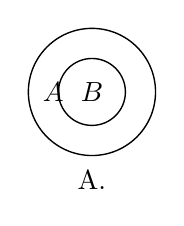
\begin{tikzpicture}[scale=0.85,line width=0.5pt]
\draw (0.9,0.9) circle (0.95);
\draw (0.9,0.9) circle (0.5);
\node at (0.32,0.9) {$A$};
\node at (0.9,0.9) {$B$};
\node[anchor=north] at (0.9,-0.12) {A.};
\end{tikzpicture}
&
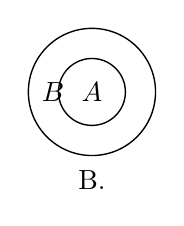
\begin{tikzpicture}[scale=0.85,line width=0.5pt]
\draw (0.9,0.9) circle (0.95);
\draw (0.9,0.9) circle (0.5);
\node at (0.32,0.9) {$B$};
\node at (0.9,0.9) {$A$};
\node[anchor=north] at (0.9,-0.12) {B.};
\end{tikzpicture}
\\[12pt]
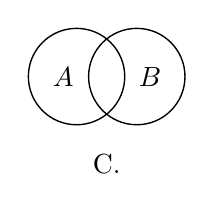
\begin{tikzpicture}[scale=0.85,line width=0.5pt]
\draw (0.65,0.9) circle (0.72);
\draw (1.55,0.9) circle (0.72);
\node at (0.45,0.9) {$A$};
\node at (1.75,0.9) {$B$};
\node[anchor=north] at (1.1,-0.12) {C.};
\end{tikzpicture}
&
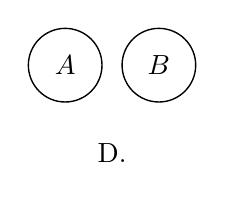
\begin{tikzpicture}[scale=0.85,line width=0.5pt]
\draw (0.55,0.9) circle (0.55);
\draw (1.95,0.9) circle (0.55);
\node at (0.55,0.9) {$A$};
\node at (1.95,0.9) {$B$};
\node[anchor=north] at (1.25,-0.12) {D.};
\end{tikzpicture}
\end{tabular}
\end{center}

\ifanswer
\solbegin
\step{$B\subset A$，图形能表示 $A$ 与 $B$ 关系的是 $A$. 故选 $A$.}
\solend
\fi

\item 以某些整数为元素的集合 $P$ 具有以下性质：

（1）$P$ 中元素有正数，也有负数；（2）$P$ 中元素有奇数，也有偶数；

（3）$-1\notin P$；（4）若 $x$、$y\in P$，则 $x+y\in P$.

则下列选项哪个是正确的\mbox{（\quad）}

\keepwithprev
A. 集合 $P$ 中一定有 $0$ 但没有 $2$\qquad\qquad B. 集合 $P$ 中一定有 $0$ 可能有 $2$

C. 集合 $P$ 中可能有 $0$ 可能有 $2$\qquad\qquad D. 集合 $P$ 中既没有 $0$ 又没有 $2$

\ifanswer
\solbegin
\step{由（4）得 $x\in P$，则 $kx\in P(k$ 是正整数$)$.}
\step{由（1）可设 $x$、$y\in P$，且 $x>0$，$y<0$，则 $xy$、$(-y)x\in P$，}
\step{因而 $0=xy+(-y)x\in P$.}
\step{假设 $2\in P$，则 $2k\in P$. 由上面及（4）得 $0$，$2$，$4$，$6$，$8$，$\cdots$ 均在 $P$ 中，}
\step{故 $2k-2\in P(k$ 是正整数$)$，}
\step{不妨令 $P$ 中负数为奇数 $-2k+1(k$ 为正整数$)$，}
\step{由（4）得 $(2k-2)+(-2k+1)=-1\in P$，矛盾.}
\step{故若 $2\in P$，则 $P$ 中没有负奇数.}
\step{若 $P$ 中负数为偶数，设为 $-2k(k$ 为正整数$)$，则由（4）及 $2\in P$，}
\step{得 $-2$,$-4$,$-6$,$\cdots$ 均在 $P$ 中，即 $-2m-2\in P(m$ 为非负整数$)$，}
\step{则 $P$ 中正奇数为 $2m+1$，由（4）得 $(-2m-2)+(2m+1)=-1\in P$，矛盾.}
\step{综上，$0\in P$，$2\notin P$，故选 $A$.}
\solend
\fi

\end{enumerate}

\bigsec{三、解答题}

\begin{enumerate}
\setcounter{enumi}{16}

\item （1）已知 $a$、$b$ 为实数，比较 $a^2+b^2$ 与 $4a-2b-5$ 的值的大小.

（2）若 $-1\leqslant x+y\leqslant2$，$-2\leqslant x-y\leqslant1$，求 $x-2y$ 的范围.

\ifanswer
\solbegin
\step{（1）$a^2+b^2-(4a-2b-5)=a^2-4a+4+b^2+2b+1=(a-2)^2+(b+1)^2\geqslant0$，}
\step{故 $a^2+b^2\geqslant4a-2b-5$.}
\step{（2）设 $x-2y=m(x+y)+n(x-y)$，则 $x-2y=(m+n)x+(m-n)y$，}
\step{所以 $\begin{cases}m+n=1\\m-n=-2\end{cases}$，解得 $n=\dfrac32$，$m=-\dfrac12$，}
\step{所以 $x-2y=-\dfrac12(x+y)+\dfrac32(x-y)$，}
\step{因为 $-1\leqslant x+y\leqslant2$，$-2\leqslant x-y\leqslant1$，}
\step{所以 $-1\leqslant-\dfrac12(x+y)\leqslant\dfrac12$，$-3\leqslant\dfrac32(x-y)\leqslant\dfrac32$，}
\step{所以 $-4\leqslant-\dfrac12(x+y)+\dfrac32(x-y)\leqslant2$，即 $-4\leqslant x-2y\leqslant2$，}
\step{故 $x-2y$ 的范围是 $[-4,2]$.}
\solend
\fi

\item 已知集合 $A=\{x\mid\lvert x-2\rvert<a\}$，集合 $B=\left\{x\,\middle\vert\,\dfrac{2x-1}{x+2}<1\right\}$.

（1）若 $a=2$，求 $A\cup B$,$A\cap B$；

（2）若 $A\cap B=A$，求实数 $a$ 的取值范围.

\ifanswer
\solbegin
\step{（1）由题意得 $A=(0,4)$,$B=(-2,3)$，所以 $A\cup B=(-2,4)$,$A\cap B=(0,3)$；}
\step{（2）因为 $A\cap B=A$，所以 $A\subseteq B$，}
\step{当 $a\leqslant0$ 时，$A=\varnothing$，满足 $A\subseteq B$；}
\step{当 $a>0$ 时，$A=(2-a,2+a)$,$B=(-2,3)$，}
\step{因为 $A\subseteq B$，所以 $\begin{cases}-2\leqslant2-a\\3\geqslant2+a\end{cases}$，解得 $a\leqslant1$，即 $0<a\leqslant1$.}
\step{因此，实数 $a$ 的取值范围为 $(-\infty,1]$.}
\solend
\fi

\item 我校校园文化节即将到来，高一年级将开展“数字配对”的抽奖活动，活动规则如下：每人可以抽取一张卡片，每张卡片上都印有一个不小于 $-10$ 且不大于 $10$ 的整数，其中不含 $2$. 每张卡片数字对应一个抽奖号码，卡片上的数字减去 $2$ 所得的差，与抽奖号码减去 $3$ 所得的差，两者的乘积等于 $12$.

（1）记卡片上的数字为 $x$，卡片数字对应的抽奖号码为 $y$，请用含有卡片数字 $x$ 的式子来表示抽奖号码 $y$；

（2）当抽奖号码不小于 $3$ 且不大于 $7$ 时，抽奖者可以领取奖品. 请问抽到哪些数字的卡片可以领取奖品？请写出满足领取奖品的卡片数字所组成的集合.

\ifanswer
\solbegin
\step{（1）卡片上的数字为 $x$，对应的抽奖号码为 $y$，}
\step{由题意得 $(x-2)(y-3)=12$，因为 $x\neq2$，所以 $y=3+\dfrac{12}{x-2}$，}
\step{所以 $y=3+\dfrac{12}{x-2}(-10\leqslant x\leqslant10,x\in\Z,x\neq2)$.}
\step{（2）由（1）得 $y=3+\dfrac{12}{x-2}(-10\leqslant x\leqslant10,x\in\Z,x\neq2)$，}
\step{由抽奖条件，得 $3\leqslant3+\dfrac{12}{x-2}\leqslant7$，$x\geqslant5$，所以 $5\leqslant x\leqslant10$，$x\in\Z$，}
\step{所以可领取奖品的卡片数字为 $\{5,6,7,8,9,10\}$.}
\solend
\fi

\item （1）已知 $m\in\R$，若不等式 $(m+1)x^2-mx+m-1<0$ 的解集是空集，求 $m$ 的取值范围；

（2）命题 $P:x^2-5x+6<0$，命题 $q:x^2-4ax+3a^2<0$，若命题 $P$ 是命题 $q$ 的充分非必要条件，求实数 $a$ 的取值范围.

\ifanswer
\solbegin
\step{（1）①当 $m+1=0$，即 $m=-1$ 时，$f(x)=x-2$，不合题意；}
\step{②当 $m+1\neq0$，即 $m\neq-1$ 时，$\begin{cases}m+1>0\\\Delta=m^2-4(m+1)(m-1)\leqslant0\end{cases}$，解得 $m\geqslant\dfrac{2\sqrt3}{3}$，}
\step{所以 $m$ 的取值范围是 $\left[\dfrac{2\sqrt3}{3},+\infty\right)$；}
\step{（2）解 $x^2-5x+6<0$，因式分解得 $(x-2)(x-3)<0$，故 $P$ 的解集为 $(2,3)$，}
\step{解 $x^2-4ax+3a^2<0$，因式分解得 $(x-a)(x-3a)<0$，}
\step{因为命题 $P$ 是命题 $q$ 的充分不必要条件，所以 $(2,3)$ 是 $q$ 解集的真子集，}
\step{当 $a=0$ 时，$q$ 的解集为 $\varnothing$，不合题意，舍去；}
\step{当 $a<0$ 时，$q$ 的解集为 $(3a,a)$，$\begin{cases}3a\leqslant2\\a\geqslant3\end{cases}$，不等式组无解，舍去；}
\step{当 $a>0$ 时，$q$ 的解集为 $(a,3a)$，又因为 $(2,3)$ 是 $q$ 解集的真子集，}
\step{所以 $\begin{cases}a\leqslant2\\3a\geqslant3\end{cases}$（等号不同时取），解得 $1\leqslant a\leqslant2$；}
\step{综上，实数 $a$ 的取值范围是 $[1,2]$.}
\solend
\fi

\item 对于至少含两个元素的有限正整数集 $A$，定义它的“两两和集”为
$S(A)=\{z\mid z=x+y$，其中 $x$、$y\in A$，且 $x<y\}$.

（1）若 $A=\{1,2,4,5\}$，求 $S(A)$；

（2）已知集合 $A$ 中恰好含有四个元素，且 $S(A)=\{5,7,8,10,11,13\}$，写出所有符合条件的集合 $A$；

（3）猜想：当集合 $A$ 含有 $n$ 个元素（$n\geqslant2$）时，$S(A)$ 的元素个数最少是多少？证明你的猜想.

\ifanswer
\solbegin
\step{（1）因为 $A=\{1,2,4,5\}$，计算所有两两和并去掉重复的结果有 $3$，$5$，$6$，$7$，$9$，}
\step{所以 $S(A)=\{3,5,6,7,9\}$.}
\step{（2）设 $A=\{a,b,c,d\}$，其中 $a<b<c<d$，且 $S(A)=\{5,7,8,10,11,13\}$，}
\step{四个元素共有六种两两配对，和集恰好有六个元素，}
\step{因此六个和互不相同.}
\step{这六个数分别为 $a+b$,$a+c$,$a+d$,$b+c$,$b+d$,$c+d$，}
\step{所以这六个数从小到大，可以确定第一个数为 $a+b$，第二数为 $a+c$，}
\step{第五个数为 $b+d$，第六数为 $c+d$，}
\step{第三个数和第四个数不能确定，即 $b+c$ 和 $a+d$ 的大小不定.}
\step{所以 $a+b=5$,$a+c=7$,$b+d=11$,$c+d=13$.}
\step{由此得到 $b=5-a$,$c=7-a$,$d=6+a$，}
\step{于是 $a+d=2a+6$,$b+c=12-2a$.}
\step{其余两个数 $b+c$,$a+d$ 对应 $8$,$10$，分两种情况讨论：}
\step{①若 $b+c=8$,$a+d=10$，则 $\begin{cases}12-2a=8\\2a+6=10\end{cases}$，解得 $a=2$，}
\step{所以 $A=\{2,3,5,8\}$；}
\step{②若 $b+c=10$,$a+d=8$，则 $\begin{cases}12-2a=10\\2a+6=8\end{cases}$，解得 $a=1$，}
\step{所以 $A=\{1,4,6,7\}$；}
\step{检验得，两组均符合题意.}
\step{因此所有符合条件的集合为 $A=\{1,4,6,7\}$ 或 $A=\{2,3,5,8\}$.}
\step{（3）猜想：两两和集的元素个数的最小值为 $2n-3$. 证明如下：}
\step{将集合中的元素按从小到大排列为 $a_1<a_2<\cdots<a_n$，}
\step{当 $n=2$ 时，两两和集恰好有一个元素，结论成立.}
\step{当 $n\geqslant3$ 时，考虑下列均属于 $S(A)$ 的数，}
\step{由不等式的传递性得严格不等式：}
\step{$a_1+a_2<a_1+a_3<\cdots<a_1+a_n<a_2+a_n<\cdots<a_{n-1}+a_n$，}
\step{其中 $a_1+a_2<a_1+a_3<\cdots<a_1+a_n$ 共有 $n-1$ 个不相等的数；}
\step{$a_2+a_n<\cdots<a_{n-1}+a_n$ 共有 $n-2$ 个不相等的数，}
\step{所以一共有 $(n-1)+(n-2)=2n-3$ 个，}
\step{因此，两两和集至少含有 $2n-3$ 个元素.}
\step{再证明可以取到 $2n-3$：}
\step{对任意 $n\geqslant2$，取 $A=\{1,2,\cdots,n\}$，}
\step{所有两两和都是不小于 $3$ 且不大于 $2n-1$ 的整数，}
\step{其中，$1+2$,$1+3$,$\cdots$,$1+n$ 是从 $3$ 到 $n+1$ 的整数；}
\step{当 $n\geqslant3$ 时，$2+n$,$3+n$,$\cdots$,$(n-1)+n$ 可取到其余整数；}
\step{因此 $S(A)=\{3,4,\cdots,2n-1\}$，其元素个数为 $(2n-1)-3+1=2n-3$，}
\step{所以所求最小值为 $2n-3$.}
\solend
\fi

\end{enumerate}

\end{document}
"
%
% 原始材料：微信公众号“魔都数学加油站”文章，作者破晓，2026-11-06 17:58 发布；
% 连载“27学年高一118”，原文标题“27学年高一118——2026-2027年上海市罗店中学高一上10月月考”；
% 原文链接：https://mp.weixin.qq.com/s/4edo8awYdjmWJl153X-aDA。
% 正文为 9 张 PNG 页（第 2、3、5、9 页 2560×3620，其余 4762×6735），
% 题目下印有【解析】或【答案】，为讲评版。
% 题目、解析均据原图转录；卷面红色水印及公众号页脚未录入。
%
% 卷首标题：原卷印作“2026-2027 年罗店中学高一上 10 月月考”（公众号标题中的“上海市”
% 卷面标题行没有，本稿照卷面），年份区间按全稿惯例排 en dash；原卷未印副标题，本稿按题目内容
% 标为“集合与常用逻辑用语、不等式”。
%
% 与原卷的排版差异：
%   ① 原文从第 3 题起，填空题 3—12、选择题 13—16、解答题 17—21，共 19 题，本稿保留原题号；
%   ② 原卷每题下直接印【解析】／【答案】，本稿按全稿惯例置于答案版；第 4 题只印【答案】、
%      第 14 题把答案“$B$”印在题干括号内且无【解析】，均另提 \ans{}；其余选择题答案在
%      解析末句“故选 …”，括号内留空；
%   ③ 原卷未印副标题，本稿按“知识模块”口径补出；
%   ④ 原卷填空横线按全稿惯例排为 \blankline[4.4em]；选择题括号排 \mbox{（\quad）}、
%      选项段前按惯例加 \keepwithprev；解答题不留作答区（原卷为讲评版，与 109—117 同）；
%   ⑤ 原卷数集 $R$／$Z$ 按全稿惯例改 \R、\Z，补集照原卷上划线排 \overline{B}。
%
% 子集符号：第 6 题、第 18 题的 $\{x\mid x<1\}\subseteq\{x\mid x<3a-2\}$ 与 $A\subseteq B$
%   印有下划线，照录 \subseteq；第 15 题解析的 $B\subset A$ 印单线（真子集、无下划线），
%   按 18／96 成例照录 \subset。
%
% 判别式字形：第 20 题 (1) cases 的判别式原卷排 $\Delta$（等腰、右厚），照录 \Delta。
%
% 图与表：第 9 题题干的文氏图（矩形 $U$ 内两椭圆 $A$、$B$，阴影为 $A\cap\overline B$）
%   按原图形状用 TikZ 重绘（三版都出）；第 12 题解析的“列表”按原卷用 tabular 重排
%   （仅答案版）；第 15 题四个文氏图选项按原图形状用 TikZ 重排（三版都出）。
%
% 原卷存疑照录：第 8 题解析“$2022+3\cdot1\cdot(-1)=2026$”一行、第 11 题解析结论
%   作“必要不充分条件”而选项列“必要非充分”、第 20 题 (2) 的 cases，均照录加注。
%
% 行数核对：逐题数 \step/\stepm 条数，合计 110 条（Q3：2；Q4：0；Q5：1；Q6：2；Q7：5；
% Q8：3；Q9：2；Q10：4；Q11：4；Q12：2；Q13：3；Q14：0；Q15：1；Q16：12；Q17：9；
% Q18：6；Q19：6；Q20：11；Q21：36），与原卷印刷行逐题相等（cases／tabular／TikZ
% 图块作一个印刷行计）。第 4 题只印【答案】、第 14 题括号内印答案且无解析，均提 \ans{}，
% 不计入 \step 账。
%
\documentclass[a4paper,11pt]{article}
\usepackage{common}

\begin{document}

\examtitlest[3]{2026--2027 年罗店中学高一上 10 月月考}{集合与常用逻辑用语、不等式}

\bigsec{一、填空题}

\begin{enumerate}
\setcounter{enumi}{2}

\item 若 $2x^2+3x+5=a(2x+1)(x+1)+b$ 恒成立，则 $a-b$ 的值\blankline[4.4em].

\ifanswer
\solbegin
\step{因为 $2x^2+3x+5=a(2x+1)(x+1)+b=2ax^2+3ax+a+b$ 恒成立，}
\step{所以 $\begin{cases}2=2a\\3=3a\\5=a+b\end{cases}$，所以 $\begin{cases}a=1\\b=4\end{cases}$，故 $a-b$ 的值为 $-3$.}
\solend
\fi

\item “$a$、$b$ 中至少有一个能被 $6$ 整除”的否定形式是\blankline[4.4em].

\ifanswer
\ans{$a$、$b$ 都不能被 $6$ 整除}
\fi

\item 设集合 $A=\{1,2\}$，则满足 $A\cup B=\{1,2,3\}$ 的集合 $B$ 的个数是\blankline[4.4em].

\ifanswer
\solbegin
\step{$B=\{3\}$,$\{1,3\}$,$\{2,3\}$,$\{1,2,3\}$，个数为 $4$.}
\solend
\fi

\item 命题“若 $x<1$，则 $x<3a-2$”是真命题，求实数 $a$ 的取值范围是\blankline[4.4em].

\ifanswer
\solbegin
\step{$\alpha:x<1$,$\beta:x<3a-2$，且若 $\alpha$ 则 $\beta$ 是真命题，}
\step{则 $\{x\mid x<1\}\subseteq\{x\mid x<3a-2\}$，所以 $3a-2\geqslant1$，解得 $a\geqslant1$.}
\solend
\fi

\item 不论实数 $m$ 取什么值，点 $P(m+1,2-m)$ 一定不在第\blankline[4.4em]象限（选填“一”、“二”、“三”或“四”）.

\ifanswer
\solbegin
\step{当 $m+1>0$，$2-m>0$ 时，解得 $-1<m<2$，此时点 $P$ 在第一象限；}
\step{当 $m+1<0$，$2-m>0$ 时，解得 $m<-1$，此时点 $P$ 在第二象限；}
\step{当 $m+1<0$，$2-m<0$ 时，$m$ 无解，此时点 $P$ 不可能在第三象限；}
\step{当 $m+1>0$，$2-m<0$ 时，解得 $m>2$，此时点 $P$ 在第四象限.}
\step{故一定不在第三象限.}
\solend
\fi

\item 设 $x_1$、$x_2$ 是方程 $x^2+x-3=0$ 的两个实数根，则 $x_1^2-x_2+2022=$\blankline[4.4em].

\ifanswer
\solbegin
\step{$x_1$、$x_2$ 是方程 $x^2+x-3=0$ 的两个实数根，}
\step{得 $x_1+x_2=-1$，$x_1^2+x_1-3=0$，所以 $x_1^2=3-x_1$，}
\step{$x_1^2-x_2+2022=3-x_1-x_2+2022=2022+3\cdot1\cdot(-1)=2026$.}
\solend
\fi

\item 如图，已知全集 $U=\R$，集合 $A=\{x\mid y=\sqrt{-x^2+x+2}\}$，$B=\{x\mid x<0$ 或 $x>5\}$. 集合 $C$ 表示图中阴影区域对应的集合，则集合 $C=$\blankline[4.4em]（用区间表示）.

\begin{center}
% 原卷文氏图：矩形 U 内两椭圆 A（阴影）、B，阴影为 A\cap\overline B，按原图形状用 TikZ 重绘。
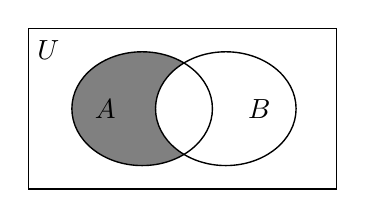
\begin{tikzpicture}[scale=0.85,line width=0.5pt]
\draw (0,0) rectangle (4.6,2.4);
\fill[gray] (1.7,1.2) ellipse (1.05 and 0.85);
\fill[white] (2.95,1.2) ellipse (1.05 and 0.85);
\draw (1.7,1.2) ellipse (1.05 and 0.85);
\draw (2.95,1.2) ellipse (1.05 and 0.85);
\node at (1.15,1.2) {$A$};
\node at (3.45,1.2) {$B$};
\node at (0.3,2.08) {$U$};
\end{tikzpicture}
\end{center}

\ifanswer
\solbegin
\step{$A=\{x\mid y=\sqrt{-x^2+x+2}\}=\{x\mid-1\leqslant x\leqslant2\}$，}
\step{$\overline B=\{x\mid 0\leqslant x\leqslant5\}$，$C=A\cap\overline B=[0,2]$.}
\solend
\fi

\item 关于 $x$ 的不等式 $ax-b<0$ 的解集为 $(2,+\infty)$，则关于 $x$ 的不等式 $(ax+b)(x-1)<0$ 的解集为\blankline[4.4em].

\ifanswer
\solbegin
\step{因为关于 $x$ 的不等式 $ax-b<0$ 的解集为 $(2,+\infty)$，所以 $\begin{cases}a<0\\2a-b=0\end{cases}$，}
\step{所以不等式 $(ax+b)(x-1)<0$ 可化为 $a\left(x+\dfrac ba\right)(x-1)<0$，$a<0$，}
\step{所以 $(x+2)(x-1)>0$，}
\step{所以所求解集为 $(-\infty,-2)\cup(1,+\infty)$.}
\solend
\fi

\item $a_1$、$b_1$、$a_2$、$b_2$ 均为非零实数，不等式 $a_1x+b_1>0$ 和 $a_2x+b_2>0$ 的解集分别为集合 $M$、$N$，那么“$\dfrac{a_1}{a_2}=\dfrac{b_1}{b_2}$”是“$M=N$”的\blankline[4.4em]条件（选填“充分非必要”、“必要非充分”、“充要”和“既非充分也非必要”）.

\ifanswer
\solbegin
\step{当 $a_1=b_1=1$，$a_2=b_2=-1$ 时，满足 $\dfrac{a_1}{a_2}=\dfrac{b_1}{b_2}$，}
\step{但是 $M=N$ 不成立，即充分性不成立；}
\step{若 $M=N$ 时，$\dfrac{a_1}{a_2}=\dfrac{b_1}{b_2}$ 一定成立，即必要性成立.}
\step{故为必要不充分条件.}% 原卷选项列“必要非充分”、解析结论作“必要不充分”，照录
\solend
\fi

\item 已知集合 $\{a,b,c\}=\{0,1,2\}$，且下列三个关系：① $a\neq2$；② $b=2$；③ $c\neq0$；有且只有一个正确，则 $100a+10b+c=$\blankline[4.4em].

\ifanswer
\solbegin
\step{列表如下：}
\begin{center}
\begin{tabular}{|c|c|c|c|c|}
\hline
 & ① & ② & ③ & \\
\hline
① 正确 & $a\neq2$ & $b\neq2$ & $c=0$ & 无解\\
\hline
② 正确 & $a=2$ & $b=2$ & $c=0$ & 矛盾\\
\hline
③ 正确 & $a=2$ & $b\neq2$ & $c\neq0$ & $a=2,b=0,c=1$\\
\hline
\end{tabular}
\end{center}
\step{所以 $100a+10b+c=201$.}
\solend
\fi

\end{enumerate}

\bigsec{二、选择题}

\begin{enumerate}
\setcounter{enumi}{12}

\item 已知 $a$,$b$,$c\in\R$,$b>c$，则下列不等式中恒成立的是\mbox{（\quad）}

\keepwithprev
A. $a+b^2>a+c^2$\qquad\quad B. $a^2+b>a^2+c$\qquad\quad C. $ab^2>ac^2$\qquad\quad D. $a^2b>a^2c$

\ifanswer
\solbegin
\step{对于 $A$，取 $b=1,c=-1$，错误；对于 $B$，由不等式的同向可加性得正确；}
\step{对于 $C$，取 $a=1,b=1,c=-2$，错误；对于 $D$，取 $a=0$，错误；}
\step{故选 $B$.}
\solend
\fi

\item 给出命题：“如果 $n$ 是素数，那么 $n^2+2$ 不是素数”，甲同学判断该命题是假命题，他做出这个判断的反例可以是\mbox{（\quad）}% 原卷把答案“$B$”印在题干括号内、无【解析】

\keepwithprev
A. $n=2$\qquad\quad B. $n=3$\qquad\quad C. $n=4$\qquad\quad D. $n=5$

\ifanswer
\ans{$B$}
\fi

\item 设集合 $A=\left\{x\,\middle\vert\,x=\dfrac n2,n\in\Z\right\}$，$B=\left\{x\,\middle\vert\,x=n+\dfrac12,n\in\Z\right\}$，则下列图形能表示 $A$ 与 $B$ 关系的是\mbox{（\quad）}

\keepwithprev
\begin{center}
% 原卷四个文氏图选项按原图形状用 TikZ 重排。
\begin{tabular}{c@{\qquad\qquad}c}
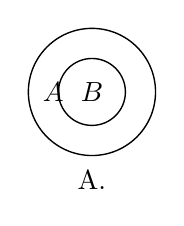
\begin{tikzpicture}[scale=0.85,line width=0.5pt]
\draw (0.9,0.9) circle (0.95);
\draw (0.9,0.9) circle (0.5);
\node at (0.32,0.9) {$A$};
\node at (0.9,0.9) {$B$};
\node[anchor=north] at (0.9,-0.12) {A.};
\end{tikzpicture}
&
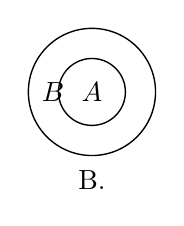
\begin{tikzpicture}[scale=0.85,line width=0.5pt]
\draw (0.9,0.9) circle (0.95);
\draw (0.9,0.9) circle (0.5);
\node at (0.32,0.9) {$B$};
\node at (0.9,0.9) {$A$};
\node[anchor=north] at (0.9,-0.12) {B.};
\end{tikzpicture}
\\[12pt]
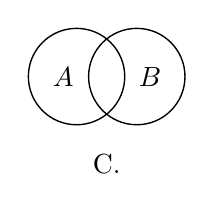
\begin{tikzpicture}[scale=0.85,line width=0.5pt]
\draw (0.65,0.9) circle (0.72);
\draw (1.55,0.9) circle (0.72);
\node at (0.45,0.9) {$A$};
\node at (1.75,0.9) {$B$};
\node[anchor=north] at (1.1,-0.12) {C.};
\end{tikzpicture}
&
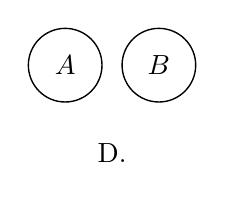
\begin{tikzpicture}[scale=0.85,line width=0.5pt]
\draw (0.55,0.9) circle (0.55);
\draw (1.95,0.9) circle (0.55);
\node at (0.55,0.9) {$A$};
\node at (1.95,0.9) {$B$};
\node[anchor=north] at (1.25,-0.12) {D.};
\end{tikzpicture}
\end{tabular}
\end{center}

\ifanswer
\solbegin
\step{$B\subset A$，图形能表示 $A$ 与 $B$ 关系的是 $A$. 故选 $A$.}
\solend
\fi

\item 以某些整数为元素的集合 $P$ 具有以下性质：

（1）$P$ 中元素有正数，也有负数；（2）$P$ 中元素有奇数，也有偶数；

（3）$-1\notin P$；（4）若 $x$、$y\in P$，则 $x+y\in P$.

则下列选项哪个是正确的\mbox{（\quad）}

\keepwithprev
A. 集合 $P$ 中一定有 $0$ 但没有 $2$\qquad\qquad B. 集合 $P$ 中一定有 $0$ 可能有 $2$

C. 集合 $P$ 中可能有 $0$ 可能有 $2$\qquad\qquad D. 集合 $P$ 中既没有 $0$ 又没有 $2$

\ifanswer
\solbegin
\step{由（4）得 $x\in P$，则 $kx\in P(k$ 是正整数$)$.}
\step{由（1）可设 $x$、$y\in P$，且 $x>0$，$y<0$，则 $xy$、$(-y)x\in P$，}
\step{因而 $0=xy+(-y)x\in P$.}
\step{假设 $2\in P$，则 $2k\in P$. 由上面及（4）得 $0$，$2$，$4$，$6$，$8$，$\cdots$ 均在 $P$ 中，}
\step{故 $2k-2\in P(k$ 是正整数$)$，}
\step{不妨令 $P$ 中负数为奇数 $-2k+1(k$ 为正整数$)$，}
\step{由（4）得 $(2k-2)+(-2k+1)=-1\in P$，矛盾.}
\step{故若 $2\in P$，则 $P$ 中没有负奇数.}
\step{若 $P$ 中负数为偶数，设为 $-2k(k$ 为正整数$)$，则由（4）及 $2\in P$，}
\step{得 $-2$,$-4$,$-6$,$\cdots$ 均在 $P$ 中，即 $-2m-2\in P(m$ 为非负整数$)$，}
\step{则 $P$ 中正奇数为 $2m+1$，由（4）得 $(-2m-2)+(2m+1)=-1\in P$，矛盾.}
\step{综上，$0\in P$，$2\notin P$，故选 $A$.}
\solend
\fi

\end{enumerate}

\bigsec{三、解答题}

\begin{enumerate}
\setcounter{enumi}{16}

\item （1）已知 $a$、$b$ 为实数，比较 $a^2+b^2$ 与 $4a-2b-5$ 的值的大小.

（2）若 $-1\leqslant x+y\leqslant2$，$-2\leqslant x-y\leqslant1$，求 $x-2y$ 的范围.

\ifanswer
\solbegin
\step{（1）$a^2+b^2-(4a-2b-5)=a^2-4a+4+b^2+2b+1=(a-2)^2+(b+1)^2\geqslant0$，}
\step{故 $a^2+b^2\geqslant4a-2b-5$.}
\step{（2）设 $x-2y=m(x+y)+n(x-y)$，则 $x-2y=(m+n)x+(m-n)y$，}
\step{所以 $\begin{cases}m+n=1\\m-n=-2\end{cases}$，解得 $n=\dfrac32$，$m=-\dfrac12$，}
\step{所以 $x-2y=-\dfrac12(x+y)+\dfrac32(x-y)$，}
\step{因为 $-1\leqslant x+y\leqslant2$，$-2\leqslant x-y\leqslant1$，}
\step{所以 $-1\leqslant-\dfrac12(x+y)\leqslant\dfrac12$，$-3\leqslant\dfrac32(x-y)\leqslant\dfrac32$，}
\step{所以 $-4\leqslant-\dfrac12(x+y)+\dfrac32(x-y)\leqslant2$，即 $-4\leqslant x-2y\leqslant2$，}
\step{故 $x-2y$ 的范围是 $[-4,2]$.}
\solend
\fi

\item 已知集合 $A=\{x\mid\lvert x-2\rvert<a\}$，集合 $B=\left\{x\,\middle\vert\,\dfrac{2x-1}{x+2}<1\right\}$.

（1）若 $a=2$，求 $A\cup B$,$A\cap B$；

（2）若 $A\cap B=A$，求实数 $a$ 的取值范围.

\ifanswer
\solbegin
\step{（1）由题意得 $A=(0,4)$,$B=(-2,3)$，所以 $A\cup B=(-2,4)$,$A\cap B=(0,3)$；}
\step{（2）因为 $A\cap B=A$，所以 $A\subseteq B$，}
\step{当 $a\leqslant0$ 时，$A=\varnothing$，满足 $A\subseteq B$；}
\step{当 $a>0$ 时，$A=(2-a,2+a)$,$B=(-2,3)$，}
\step{因为 $A\subseteq B$，所以 $\begin{cases}-2\leqslant2-a\\3\geqslant2+a\end{cases}$，解得 $a\leqslant1$，即 $0<a\leqslant1$.}
\step{因此，实数 $a$ 的取值范围为 $(-\infty,1]$.}
\solend
\fi

\item 我校校园文化节即将到来，高一年级将开展“数字配对”的抽奖活动，活动规则如下：每人可以抽取一张卡片，每张卡片上都印有一个不小于 $-10$ 且不大于 $10$ 的整数，其中不含 $2$. 每张卡片数字对应一个抽奖号码，卡片上的数字减去 $2$ 所得的差，与抽奖号码减去 $3$ 所得的差，两者的乘积等于 $12$.

（1）记卡片上的数字为 $x$，卡片数字对应的抽奖号码为 $y$，请用含有卡片数字 $x$ 的式子来表示抽奖号码 $y$；

（2）当抽奖号码不小于 $3$ 且不大于 $7$ 时，抽奖者可以领取奖品. 请问抽到哪些数字的卡片可以领取奖品？请写出满足领取奖品的卡片数字所组成的集合.

\ifanswer
\solbegin
\step{（1）卡片上的数字为 $x$，对应的抽奖号码为 $y$，}
\step{由题意得 $(x-2)(y-3)=12$，因为 $x\neq2$，所以 $y=3+\dfrac{12}{x-2}$，}
\step{所以 $y=3+\dfrac{12}{x-2}(-10\leqslant x\leqslant10,x\in\Z,x\neq2)$.}
\step{（2）由（1）得 $y=3+\dfrac{12}{x-2}(-10\leqslant x\leqslant10,x\in\Z,x\neq2)$，}
\step{由抽奖条件，得 $3\leqslant3+\dfrac{12}{x-2}\leqslant7$，$x\geqslant5$，所以 $5\leqslant x\leqslant10$，$x\in\Z$，}
\step{所以可领取奖品的卡片数字为 $\{5,6,7,8,9,10\}$.}
\solend
\fi

\item （1）已知 $m\in\R$，若不等式 $(m+1)x^2-mx+m-1<0$ 的解集是空集，求 $m$ 的取值范围；

（2）命题 $P:x^2-5x+6<0$，命题 $q:x^2-4ax+3a^2<0$，若命题 $P$ 是命题 $q$ 的充分非必要条件，求实数 $a$ 的取值范围.

\ifanswer
\solbegin
\step{（1）①当 $m+1=0$，即 $m=-1$ 时，$f(x)=x-2$，不合题意；}
\step{②当 $m+1\neq0$，即 $m\neq-1$ 时，$\begin{cases}m+1>0\\\Delta=m^2-4(m+1)(m-1)\leqslant0\end{cases}$，解得 $m\geqslant\dfrac{2\sqrt3}{3}$，}
\step{所以 $m$ 的取值范围是 $\left[\dfrac{2\sqrt3}{3},+\infty\right)$；}
\step{（2）解 $x^2-5x+6<0$，因式分解得 $(x-2)(x-3)<0$，故 $P$ 的解集为 $(2,3)$，}
\step{解 $x^2-4ax+3a^2<0$，因式分解得 $(x-a)(x-3a)<0$，}
\step{因为命题 $P$ 是命题 $q$ 的充分不必要条件，所以 $(2,3)$ 是 $q$ 解集的真子集，}
\step{当 $a=0$ 时，$q$ 的解集为 $\varnothing$，不合题意，舍去；}
\step{当 $a<0$ 时，$q$ 的解集为 $(3a,a)$，$\begin{cases}3a\leqslant2\\a\geqslant3\end{cases}$，不等式组无解，舍去；}
\step{当 $a>0$ 时，$q$ 的解集为 $(a,3a)$，又因为 $(2,3)$ 是 $q$ 解集的真子集，}
\step{所以 $\begin{cases}a\leqslant2\\3a\geqslant3\end{cases}$（等号不同时取），解得 $1\leqslant a\leqslant2$；}
\step{综上，实数 $a$ 的取值范围是 $[1,2]$.}
\solend
\fi

\item 对于至少含两个元素的有限正整数集 $A$，定义它的“两两和集”为
$S(A)=\{z\mid z=x+y$，其中 $x$、$y\in A$，且 $x<y\}$.

（1）若 $A=\{1,2,4,5\}$，求 $S(A)$；

（2）已知集合 $A$ 中恰好含有四个元素，且 $S(A)=\{5,7,8,10,11,13\}$，写出所有符合条件的集合 $A$；

（3）猜想：当集合 $A$ 含有 $n$ 个元素（$n\geqslant2$）时，$S(A)$ 的元素个数最少是多少？证明你的猜想.

\ifanswer
\solbegin
\step{（1）因为 $A=\{1,2,4,5\}$，计算所有两两和并去掉重复的结果有 $3$，$5$，$6$，$7$，$9$，}
\step{所以 $S(A)=\{3,5,6,7,9\}$.}
\step{（2）设 $A=\{a,b,c,d\}$，其中 $a<b<c<d$，且 $S(A)=\{5,7,8,10,11,13\}$，}
\step{四个元素共有六种两两配对，和集恰好有六个元素，}
\step{因此六个和互不相同.}
\step{这六个数分别为 $a+b$,$a+c$,$a+d$,$b+c$,$b+d$,$c+d$，}
\step{所以这六个数从小到大，可以确定第一个数为 $a+b$，第二数为 $a+c$，}
\step{第五个数为 $b+d$，第六数为 $c+d$，}
\step{第三个数和第四个数不能确定，即 $b+c$ 和 $a+d$ 的大小不定.}
\step{所以 $a+b=5$,$a+c=7$,$b+d=11$,$c+d=13$.}
\step{由此得到 $b=5-a$,$c=7-a$,$d=6+a$，}
\step{于是 $a+d=2a+6$,$b+c=12-2a$.}
\step{其余两个数 $b+c$,$a+d$ 对应 $8$,$10$，分两种情况讨论：}
\step{①若 $b+c=8$,$a+d=10$，则 $\begin{cases}12-2a=8\\2a+6=10\end{cases}$，解得 $a=2$，}
\step{所以 $A=\{2,3,5,8\}$；}
\step{②若 $b+c=10$,$a+d=8$，则 $\begin{cases}12-2a=10\\2a+6=8\end{cases}$，解得 $a=1$，}
\step{所以 $A=\{1,4,6,7\}$；}
\step{检验得，两组均符合题意.}
\step{因此所有符合条件的集合为 $A=\{1,4,6,7\}$ 或 $A=\{2,3,5,8\}$.}
\step{（3）猜想：两两和集的元素个数的最小值为 $2n-3$. 证明如下：}
\step{将集合中的元素按从小到大排列为 $a_1<a_2<\cdots<a_n$，}
\step{当 $n=2$ 时，两两和集恰好有一个元素，结论成立.}
\step{当 $n\geqslant3$ 时，考虑下列均属于 $S(A)$ 的数，}
\step{由不等式的传递性得严格不等式：}
\step{$a_1+a_2<a_1+a_3<\cdots<a_1+a_n<a_2+a_n<\cdots<a_{n-1}+a_n$，}
\step{其中 $a_1+a_2<a_1+a_3<\cdots<a_1+a_n$ 共有 $n-1$ 个不相等的数；}
\step{$a_2+a_n<\cdots<a_{n-1}+a_n$ 共有 $n-2$ 个不相等的数，}
\step{所以一共有 $(n-1)+(n-2)=2n-3$ 个，}
\step{因此，两两和集至少含有 $2n-3$ 个元素.}
\step{再证明可以取到 $2n-3$：}
\step{对任意 $n\geqslant2$，取 $A=\{1,2,\cdots,n\}$，}
\step{所有两两和都是不小于 $3$ 且不大于 $2n-1$ 的整数，}
\step{其中，$1+2$,$1+3$,$\cdots$,$1+n$ 是从 $3$ 到 $n+1$ 的整数；}
\step{当 $n\geqslant3$ 时，$2+n$,$3+n$,$\cdots$,$(n-1)+n$ 可取到其余整数；}
\step{因此 $S(A)=\{3,4,\cdots,2n-1\}$，其元素个数为 $(2n-1)-3+1=2n-3$，}
\step{所以所求最小值为 $2n-3$.}
\solend
\fi

\end{enumerate}

\end{document}
"
% 紧凑版：xelatex "\def\iscompact{1}% 高一118_罗店中学_10月月考.tex
%   —— 高一上数学“2026-2027 年罗店中学高一上 10 月月考”（试卷版/答案版）
% 试卷版：xelatex 高一118_罗店中学_10月月考.tex
% 答案版：xelatex "\def\isanswer{1}% 高一118_罗店中学_10月月考.tex
%   —— 高一上数学“2026-2027 年罗店中学高一上 10 月月考”（试卷版/答案版）
% 试卷版：xelatex 高一118_罗店中学_10月月考.tex
% 答案版：xelatex "\def\isanswer{1}\input{高一118_罗店中学_10月月考.tex}"
% 紧凑版：xelatex "\def\iscompact{1}\input{高一118_罗店中学_10月月考.tex}"
%
% 原始材料：微信公众号“魔都数学加油站”文章，作者破晓，2026-11-06 17:58 发布；
% 连载“27学年高一118”，原文标题“27学年高一118——2026-2027年上海市罗店中学高一上10月月考”；
% 原文链接：https://mp.weixin.qq.com/s/4edo8awYdjmWJl153X-aDA。
% 正文为 9 张 PNG 页（第 2、3、5、9 页 2560×3620，其余 4762×6735），
% 题目下印有【解析】或【答案】，为讲评版。
% 题目、解析均据原图转录；卷面红色水印及公众号页脚未录入。
%
% 卷首标题：原卷印作“2026-2027 年罗店中学高一上 10 月月考”（公众号标题中的“上海市”
% 卷面标题行没有，本稿照卷面），年份区间按全稿惯例排 en dash；原卷未印副标题，本稿按题目内容
% 标为“集合与常用逻辑用语、不等式”。
%
% 与原卷的排版差异：
%   ① 原文从第 3 题起，填空题 3—12、选择题 13—16、解答题 17—21，共 19 题，本稿保留原题号；
%   ② 原卷每题下直接印【解析】／【答案】，本稿按全稿惯例置于答案版；第 4 题只印【答案】、
%      第 14 题把答案“$B$”印在题干括号内且无【解析】，均另提 \ans{}；其余选择题答案在
%      解析末句“故选 …”，括号内留空；
%   ③ 原卷未印副标题，本稿按“知识模块”口径补出；
%   ④ 原卷填空横线按全稿惯例排为 \blankline[4.4em]；选择题括号排 \mbox{（\quad）}、
%      选项段前按惯例加 \keepwithprev；解答题不留作答区（原卷为讲评版，与 109—117 同）；
%   ⑤ 原卷数集 $R$／$Z$ 按全稿惯例改 \R、\Z，补集照原卷上划线排 \overline{B}。
%
% 子集符号：第 6 题、第 18 题的 $\{x\mid x<1\}\subseteq\{x\mid x<3a-2\}$ 与 $A\subseteq B$
%   印有下划线，照录 \subseteq；第 15 题解析的 $B\subset A$ 印单线（真子集、无下划线），
%   按 18／96 成例照录 \subset。
%
% 判别式字形：第 20 题 (1) cases 的判别式原卷排 $\Delta$（等腰、右厚），照录 \Delta。
%
% 图与表：第 9 题题干的文氏图（矩形 $U$ 内两椭圆 $A$、$B$，阴影为 $A\cap\overline B$）
%   按原图形状用 TikZ 重绘（三版都出）；第 12 题解析的“列表”按原卷用 tabular 重排
%   （仅答案版）；第 15 题四个文氏图选项按原图形状用 TikZ 重排（三版都出）。
%
% 原卷存疑照录：第 8 题解析“$2022+3\cdot1\cdot(-1)=2026$”一行、第 11 题解析结论
%   作“必要不充分条件”而选项列“必要非充分”、第 20 题 (2) 的 cases，均照录加注。
%
% 行数核对：逐题数 \step/\stepm 条数，合计 110 条（Q3：2；Q4：0；Q5：1；Q6：2；Q7：5；
% Q8：3；Q9：2；Q10：4；Q11：4；Q12：2；Q13：3；Q14：0；Q15：1；Q16：12；Q17：9；
% Q18：6；Q19：6；Q20：11；Q21：36），与原卷印刷行逐题相等（cases／tabular／TikZ
% 图块作一个印刷行计）。第 4 题只印【答案】、第 14 题括号内印答案且无解析，均提 \ans{}，
% 不计入 \step 账。
%
\documentclass[a4paper,11pt]{article}
\usepackage{common}

\begin{document}

\examtitlest[3]{2026--2027 年罗店中学高一上 10 月月考}{集合与常用逻辑用语、不等式}

\bigsec{一、填空题}

\begin{enumerate}
\setcounter{enumi}{2}

\item 若 $2x^2+3x+5=a(2x+1)(x+1)+b$ 恒成立，则 $a-b$ 的值\blankline[4.4em].

\ifanswer
\solbegin
\step{因为 $2x^2+3x+5=a(2x+1)(x+1)+b=2ax^2+3ax+a+b$ 恒成立，}
\step{所以 $\begin{cases}2=2a\\3=3a\\5=a+b\end{cases}$，所以 $\begin{cases}a=1\\b=4\end{cases}$，故 $a-b$ 的值为 $-3$.}
\solend
\fi

\item “$a$、$b$ 中至少有一个能被 $6$ 整除”的否定形式是\blankline[4.4em].

\ifanswer
\ans{$a$、$b$ 都不能被 $6$ 整除}
\fi

\item 设集合 $A=\{1,2\}$，则满足 $A\cup B=\{1,2,3\}$ 的集合 $B$ 的个数是\blankline[4.4em].

\ifanswer
\solbegin
\step{$B=\{3\}$,$\{1,3\}$,$\{2,3\}$,$\{1,2,3\}$，个数为 $4$.}
\solend
\fi

\item 命题“若 $x<1$，则 $x<3a-2$”是真命题，求实数 $a$ 的取值范围是\blankline[4.4em].

\ifanswer
\solbegin
\step{$\alpha:x<1$,$\beta:x<3a-2$，且若 $\alpha$ 则 $\beta$ 是真命题，}
\step{则 $\{x\mid x<1\}\subseteq\{x\mid x<3a-2\}$，所以 $3a-2\geqslant1$，解得 $a\geqslant1$.}
\solend
\fi

\item 不论实数 $m$ 取什么值，点 $P(m+1,2-m)$ 一定不在第\blankline[4.4em]象限（选填“一”、“二”、“三”或“四”）.

\ifanswer
\solbegin
\step{当 $m+1>0$，$2-m>0$ 时，解得 $-1<m<2$，此时点 $P$ 在第一象限；}
\step{当 $m+1<0$，$2-m>0$ 时，解得 $m<-1$，此时点 $P$ 在第二象限；}
\step{当 $m+1<0$，$2-m<0$ 时，$m$ 无解，此时点 $P$ 不可能在第三象限；}
\step{当 $m+1>0$，$2-m<0$ 时，解得 $m>2$，此时点 $P$ 在第四象限.}
\step{故一定不在第三象限.}
\solend
\fi

\item 设 $x_1$、$x_2$ 是方程 $x^2+x-3=0$ 的两个实数根，则 $x_1^2-x_2+2022=$\blankline[4.4em].

\ifanswer
\solbegin
\step{$x_1$、$x_2$ 是方程 $x^2+x-3=0$ 的两个实数根，}
\step{得 $x_1+x_2=-1$，$x_1^2+x_1-3=0$，所以 $x_1^2=3-x_1$，}
\step{$x_1^2-x_2+2022=3-x_1-x_2+2022=2022+3\cdot1\cdot(-1)=2026$.}
\solend
\fi

\item 如图，已知全集 $U=\R$，集合 $A=\{x\mid y=\sqrt{-x^2+x+2}\}$，$B=\{x\mid x<0$ 或 $x>5\}$. 集合 $C$ 表示图中阴影区域对应的集合，则集合 $C=$\blankline[4.4em]（用区间表示）.

\begin{center}
% 原卷文氏图：矩形 U 内两椭圆 A（阴影）、B，阴影为 A\cap\overline B，按原图形状用 TikZ 重绘。
\begin{tikzpicture}[scale=0.85,line width=0.5pt]
\draw (0,0) rectangle (4.6,2.4);
\fill[gray] (1.7,1.2) ellipse (1.05 and 0.85);
\fill[white] (2.95,1.2) ellipse (1.05 and 0.85);
\draw (1.7,1.2) ellipse (1.05 and 0.85);
\draw (2.95,1.2) ellipse (1.05 and 0.85);
\node at (1.15,1.2) {$A$};
\node at (3.45,1.2) {$B$};
\node at (0.3,2.08) {$U$};
\end{tikzpicture}
\end{center}

\ifanswer
\solbegin
\step{$A=\{x\mid y=\sqrt{-x^2+x+2}\}=\{x\mid-1\leqslant x\leqslant2\}$，}
\step{$\overline B=\{x\mid 0\leqslant x\leqslant5\}$，$C=A\cap\overline B=[0,2]$.}
\solend
\fi

\item 关于 $x$ 的不等式 $ax-b<0$ 的解集为 $(2,+\infty)$，则关于 $x$ 的不等式 $(ax+b)(x-1)<0$ 的解集为\blankline[4.4em].

\ifanswer
\solbegin
\step{因为关于 $x$ 的不等式 $ax-b<0$ 的解集为 $(2,+\infty)$，所以 $\begin{cases}a<0\\2a-b=0\end{cases}$，}
\step{所以不等式 $(ax+b)(x-1)<0$ 可化为 $a\left(x+\dfrac ba\right)(x-1)<0$，$a<0$，}
\step{所以 $(x+2)(x-1)>0$，}
\step{所以所求解集为 $(-\infty,-2)\cup(1,+\infty)$.}
\solend
\fi

\item $a_1$、$b_1$、$a_2$、$b_2$ 均为非零实数，不等式 $a_1x+b_1>0$ 和 $a_2x+b_2>0$ 的解集分别为集合 $M$、$N$，那么“$\dfrac{a_1}{a_2}=\dfrac{b_1}{b_2}$”是“$M=N$”的\blankline[4.4em]条件（选填“充分非必要”、“必要非充分”、“充要”和“既非充分也非必要”）.

\ifanswer
\solbegin
\step{当 $a_1=b_1=1$，$a_2=b_2=-1$ 时，满足 $\dfrac{a_1}{a_2}=\dfrac{b_1}{b_2}$，}
\step{但是 $M=N$ 不成立，即充分性不成立；}
\step{若 $M=N$ 时，$\dfrac{a_1}{a_2}=\dfrac{b_1}{b_2}$ 一定成立，即必要性成立.}
\step{故为必要不充分条件.}% 原卷选项列“必要非充分”、解析结论作“必要不充分”，照录
\solend
\fi

\item 已知集合 $\{a,b,c\}=\{0,1,2\}$，且下列三个关系：① $a\neq2$；② $b=2$；③ $c\neq0$；有且只有一个正确，则 $100a+10b+c=$\blankline[4.4em].

\ifanswer
\solbegin
\step{列表如下：}
\begin{center}
\begin{tabular}{|c|c|c|c|c|}
\hline
 & ① & ② & ③ & \\
\hline
① 正确 & $a\neq2$ & $b\neq2$ & $c=0$ & 无解\\
\hline
② 正确 & $a=2$ & $b=2$ & $c=0$ & 矛盾\\
\hline
③ 正确 & $a=2$ & $b\neq2$ & $c\neq0$ & $a=2,b=0,c=1$\\
\hline
\end{tabular}
\end{center}
\step{所以 $100a+10b+c=201$.}
\solend
\fi

\end{enumerate}

\bigsec{二、选择题}

\begin{enumerate}
\setcounter{enumi}{12}

\item 已知 $a$,$b$,$c\in\R$,$b>c$，则下列不等式中恒成立的是\mbox{（\quad）}

\keepwithprev
A. $a+b^2>a+c^2$\qquad\quad B. $a^2+b>a^2+c$\qquad\quad C. $ab^2>ac^2$\qquad\quad D. $a^2b>a^2c$

\ifanswer
\solbegin
\step{对于 $A$，取 $b=1,c=-1$，错误；对于 $B$，由不等式的同向可加性得正确；}
\step{对于 $C$，取 $a=1,b=1,c=-2$，错误；对于 $D$，取 $a=0$，错误；}
\step{故选 $B$.}
\solend
\fi

\item 给出命题：“如果 $n$ 是素数，那么 $n^2+2$ 不是素数”，甲同学判断该命题是假命题，他做出这个判断的反例可以是\mbox{（\quad）}% 原卷把答案“$B$”印在题干括号内、无【解析】

\keepwithprev
A. $n=2$\qquad\quad B. $n=3$\qquad\quad C. $n=4$\qquad\quad D. $n=5$

\ifanswer
\ans{$B$}
\fi

\item 设集合 $A=\left\{x\,\middle\vert\,x=\dfrac n2,n\in\Z\right\}$，$B=\left\{x\,\middle\vert\,x=n+\dfrac12,n\in\Z\right\}$，则下列图形能表示 $A$ 与 $B$ 关系的是\mbox{（\quad）}

\keepwithprev
\begin{center}
% 原卷四个文氏图选项按原图形状用 TikZ 重排。
\begin{tabular}{c@{\qquad\qquad}c}
\begin{tikzpicture}[scale=0.85,line width=0.5pt]
\draw (0.9,0.9) circle (0.95);
\draw (0.9,0.9) circle (0.5);
\node at (0.32,0.9) {$A$};
\node at (0.9,0.9) {$B$};
\node[anchor=north] at (0.9,-0.12) {A.};
\end{tikzpicture}
&
\begin{tikzpicture}[scale=0.85,line width=0.5pt]
\draw (0.9,0.9) circle (0.95);
\draw (0.9,0.9) circle (0.5);
\node at (0.32,0.9) {$B$};
\node at (0.9,0.9) {$A$};
\node[anchor=north] at (0.9,-0.12) {B.};
\end{tikzpicture}
\\[12pt]
\begin{tikzpicture}[scale=0.85,line width=0.5pt]
\draw (0.65,0.9) circle (0.72);
\draw (1.55,0.9) circle (0.72);
\node at (0.45,0.9) {$A$};
\node at (1.75,0.9) {$B$};
\node[anchor=north] at (1.1,-0.12) {C.};
\end{tikzpicture}
&
\begin{tikzpicture}[scale=0.85,line width=0.5pt]
\draw (0.55,0.9) circle (0.55);
\draw (1.95,0.9) circle (0.55);
\node at (0.55,0.9) {$A$};
\node at (1.95,0.9) {$B$};
\node[anchor=north] at (1.25,-0.12) {D.};
\end{tikzpicture}
\end{tabular}
\end{center}

\ifanswer
\solbegin
\step{$B\subset A$，图形能表示 $A$ 与 $B$ 关系的是 $A$. 故选 $A$.}
\solend
\fi

\item 以某些整数为元素的集合 $P$ 具有以下性质：

（1）$P$ 中元素有正数，也有负数；（2）$P$ 中元素有奇数，也有偶数；

（3）$-1\notin P$；（4）若 $x$、$y\in P$，则 $x+y\in P$.

则下列选项哪个是正确的\mbox{（\quad）}

\keepwithprev
A. 集合 $P$ 中一定有 $0$ 但没有 $2$\qquad\qquad B. 集合 $P$ 中一定有 $0$ 可能有 $2$

C. 集合 $P$ 中可能有 $0$ 可能有 $2$\qquad\qquad D. 集合 $P$ 中既没有 $0$ 又没有 $2$

\ifanswer
\solbegin
\step{由（4）得 $x\in P$，则 $kx\in P(k$ 是正整数$)$.}
\step{由（1）可设 $x$、$y\in P$，且 $x>0$，$y<0$，则 $xy$、$(-y)x\in P$，}
\step{因而 $0=xy+(-y)x\in P$.}
\step{假设 $2\in P$，则 $2k\in P$. 由上面及（4）得 $0$，$2$，$4$，$6$，$8$，$\cdots$ 均在 $P$ 中，}
\step{故 $2k-2\in P(k$ 是正整数$)$，}
\step{不妨令 $P$ 中负数为奇数 $-2k+1(k$ 为正整数$)$，}
\step{由（4）得 $(2k-2)+(-2k+1)=-1\in P$，矛盾.}
\step{故若 $2\in P$，则 $P$ 中没有负奇数.}
\step{若 $P$ 中负数为偶数，设为 $-2k(k$ 为正整数$)$，则由（4）及 $2\in P$，}
\step{得 $-2$,$-4$,$-6$,$\cdots$ 均在 $P$ 中，即 $-2m-2\in P(m$ 为非负整数$)$，}
\step{则 $P$ 中正奇数为 $2m+1$，由（4）得 $(-2m-2)+(2m+1)=-1\in P$，矛盾.}
\step{综上，$0\in P$，$2\notin P$，故选 $A$.}
\solend
\fi

\end{enumerate}

\bigsec{三、解答题}

\begin{enumerate}
\setcounter{enumi}{16}

\item （1）已知 $a$、$b$ 为实数，比较 $a^2+b^2$ 与 $4a-2b-5$ 的值的大小.

（2）若 $-1\leqslant x+y\leqslant2$，$-2\leqslant x-y\leqslant1$，求 $x-2y$ 的范围.

\ifanswer
\solbegin
\step{（1）$a^2+b^2-(4a-2b-5)=a^2-4a+4+b^2+2b+1=(a-2)^2+(b+1)^2\geqslant0$，}
\step{故 $a^2+b^2\geqslant4a-2b-5$.}
\step{（2）设 $x-2y=m(x+y)+n(x-y)$，则 $x-2y=(m+n)x+(m-n)y$，}
\step{所以 $\begin{cases}m+n=1\\m-n=-2\end{cases}$，解得 $n=\dfrac32$，$m=-\dfrac12$，}
\step{所以 $x-2y=-\dfrac12(x+y)+\dfrac32(x-y)$，}
\step{因为 $-1\leqslant x+y\leqslant2$，$-2\leqslant x-y\leqslant1$，}
\step{所以 $-1\leqslant-\dfrac12(x+y)\leqslant\dfrac12$，$-3\leqslant\dfrac32(x-y)\leqslant\dfrac32$，}
\step{所以 $-4\leqslant-\dfrac12(x+y)+\dfrac32(x-y)\leqslant2$，即 $-4\leqslant x-2y\leqslant2$，}
\step{故 $x-2y$ 的范围是 $[-4,2]$.}
\solend
\fi

\item 已知集合 $A=\{x\mid\lvert x-2\rvert<a\}$，集合 $B=\left\{x\,\middle\vert\,\dfrac{2x-1}{x+2}<1\right\}$.

（1）若 $a=2$，求 $A\cup B$,$A\cap B$；

（2）若 $A\cap B=A$，求实数 $a$ 的取值范围.

\ifanswer
\solbegin
\step{（1）由题意得 $A=(0,4)$,$B=(-2,3)$，所以 $A\cup B=(-2,4)$,$A\cap B=(0,3)$；}
\step{（2）因为 $A\cap B=A$，所以 $A\subseteq B$，}
\step{当 $a\leqslant0$ 时，$A=\varnothing$，满足 $A\subseteq B$；}
\step{当 $a>0$ 时，$A=(2-a,2+a)$,$B=(-2,3)$，}
\step{因为 $A\subseteq B$，所以 $\begin{cases}-2\leqslant2-a\\3\geqslant2+a\end{cases}$，解得 $a\leqslant1$，即 $0<a\leqslant1$.}
\step{因此，实数 $a$ 的取值范围为 $(-\infty,1]$.}
\solend
\fi

\item 我校校园文化节即将到来，高一年级将开展“数字配对”的抽奖活动，活动规则如下：每人可以抽取一张卡片，每张卡片上都印有一个不小于 $-10$ 且不大于 $10$ 的整数，其中不含 $2$. 每张卡片数字对应一个抽奖号码，卡片上的数字减去 $2$ 所得的差，与抽奖号码减去 $3$ 所得的差，两者的乘积等于 $12$.

（1）记卡片上的数字为 $x$，卡片数字对应的抽奖号码为 $y$，请用含有卡片数字 $x$ 的式子来表示抽奖号码 $y$；

（2）当抽奖号码不小于 $3$ 且不大于 $7$ 时，抽奖者可以领取奖品. 请问抽到哪些数字的卡片可以领取奖品？请写出满足领取奖品的卡片数字所组成的集合.

\ifanswer
\solbegin
\step{（1）卡片上的数字为 $x$，对应的抽奖号码为 $y$，}
\step{由题意得 $(x-2)(y-3)=12$，因为 $x\neq2$，所以 $y=3+\dfrac{12}{x-2}$，}
\step{所以 $y=3+\dfrac{12}{x-2}(-10\leqslant x\leqslant10,x\in\Z,x\neq2)$.}
\step{（2）由（1）得 $y=3+\dfrac{12}{x-2}(-10\leqslant x\leqslant10,x\in\Z,x\neq2)$，}
\step{由抽奖条件，得 $3\leqslant3+\dfrac{12}{x-2}\leqslant7$，$x\geqslant5$，所以 $5\leqslant x\leqslant10$，$x\in\Z$，}
\step{所以可领取奖品的卡片数字为 $\{5,6,7,8,9,10\}$.}
\solend
\fi

\item （1）已知 $m\in\R$，若不等式 $(m+1)x^2-mx+m-1<0$ 的解集是空集，求 $m$ 的取值范围；

（2）命题 $P:x^2-5x+6<0$，命题 $q:x^2-4ax+3a^2<0$，若命题 $P$ 是命题 $q$ 的充分非必要条件，求实数 $a$ 的取值范围.

\ifanswer
\solbegin
\step{（1）①当 $m+1=0$，即 $m=-1$ 时，$f(x)=x-2$，不合题意；}
\step{②当 $m+1\neq0$，即 $m\neq-1$ 时，$\begin{cases}m+1>0\\\Delta=m^2-4(m+1)(m-1)\leqslant0\end{cases}$，解得 $m\geqslant\dfrac{2\sqrt3}{3}$，}
\step{所以 $m$ 的取值范围是 $\left[\dfrac{2\sqrt3}{3},+\infty\right)$；}
\step{（2）解 $x^2-5x+6<0$，因式分解得 $(x-2)(x-3)<0$，故 $P$ 的解集为 $(2,3)$，}
\step{解 $x^2-4ax+3a^2<0$，因式分解得 $(x-a)(x-3a)<0$，}
\step{因为命题 $P$ 是命题 $q$ 的充分不必要条件，所以 $(2,3)$ 是 $q$ 解集的真子集，}
\step{当 $a=0$ 时，$q$ 的解集为 $\varnothing$，不合题意，舍去；}
\step{当 $a<0$ 时，$q$ 的解集为 $(3a,a)$，$\begin{cases}3a\leqslant2\\a\geqslant3\end{cases}$，不等式组无解，舍去；}
\step{当 $a>0$ 时，$q$ 的解集为 $(a,3a)$，又因为 $(2,3)$ 是 $q$ 解集的真子集，}
\step{所以 $\begin{cases}a\leqslant2\\3a\geqslant3\end{cases}$（等号不同时取），解得 $1\leqslant a\leqslant2$；}
\step{综上，实数 $a$ 的取值范围是 $[1,2]$.}
\solend
\fi

\item 对于至少含两个元素的有限正整数集 $A$，定义它的“两两和集”为
$S(A)=\{z\mid z=x+y$，其中 $x$、$y\in A$，且 $x<y\}$.

（1）若 $A=\{1,2,4,5\}$，求 $S(A)$；

（2）已知集合 $A$ 中恰好含有四个元素，且 $S(A)=\{5,7,8,10,11,13\}$，写出所有符合条件的集合 $A$；

（3）猜想：当集合 $A$ 含有 $n$ 个元素（$n\geqslant2$）时，$S(A)$ 的元素个数最少是多少？证明你的猜想.

\ifanswer
\solbegin
\step{（1）因为 $A=\{1,2,4,5\}$，计算所有两两和并去掉重复的结果有 $3$，$5$，$6$，$7$，$9$，}
\step{所以 $S(A)=\{3,5,6,7,9\}$.}
\step{（2）设 $A=\{a,b,c,d\}$，其中 $a<b<c<d$，且 $S(A)=\{5,7,8,10,11,13\}$，}
\step{四个元素共有六种两两配对，和集恰好有六个元素，}
\step{因此六个和互不相同.}
\step{这六个数分别为 $a+b$,$a+c$,$a+d$,$b+c$,$b+d$,$c+d$，}
\step{所以这六个数从小到大，可以确定第一个数为 $a+b$，第二数为 $a+c$，}
\step{第五个数为 $b+d$，第六数为 $c+d$，}
\step{第三个数和第四个数不能确定，即 $b+c$ 和 $a+d$ 的大小不定.}
\step{所以 $a+b=5$,$a+c=7$,$b+d=11$,$c+d=13$.}
\step{由此得到 $b=5-a$,$c=7-a$,$d=6+a$，}
\step{于是 $a+d=2a+6$,$b+c=12-2a$.}
\step{其余两个数 $b+c$,$a+d$ 对应 $8$,$10$，分两种情况讨论：}
\step{①若 $b+c=8$,$a+d=10$，则 $\begin{cases}12-2a=8\\2a+6=10\end{cases}$，解得 $a=2$，}
\step{所以 $A=\{2,3,5,8\}$；}
\step{②若 $b+c=10$,$a+d=8$，则 $\begin{cases}12-2a=10\\2a+6=8\end{cases}$，解得 $a=1$，}
\step{所以 $A=\{1,4,6,7\}$；}
\step{检验得，两组均符合题意.}
\step{因此所有符合条件的集合为 $A=\{1,4,6,7\}$ 或 $A=\{2,3,5,8\}$.}
\step{（3）猜想：两两和集的元素个数的最小值为 $2n-3$. 证明如下：}
\step{将集合中的元素按从小到大排列为 $a_1<a_2<\cdots<a_n$，}
\step{当 $n=2$ 时，两两和集恰好有一个元素，结论成立.}
\step{当 $n\geqslant3$ 时，考虑下列均属于 $S(A)$ 的数，}
\step{由不等式的传递性得严格不等式：}
\step{$a_1+a_2<a_1+a_3<\cdots<a_1+a_n<a_2+a_n<\cdots<a_{n-1}+a_n$，}
\step{其中 $a_1+a_2<a_1+a_3<\cdots<a_1+a_n$ 共有 $n-1$ 个不相等的数；}
\step{$a_2+a_n<\cdots<a_{n-1}+a_n$ 共有 $n-2$ 个不相等的数，}
\step{所以一共有 $(n-1)+(n-2)=2n-3$ 个，}
\step{因此，两两和集至少含有 $2n-3$ 个元素.}
\step{再证明可以取到 $2n-3$：}
\step{对任意 $n\geqslant2$，取 $A=\{1,2,\cdots,n\}$，}
\step{所有两两和都是不小于 $3$ 且不大于 $2n-1$ 的整数，}
\step{其中，$1+2$,$1+3$,$\cdots$,$1+n$ 是从 $3$ 到 $n+1$ 的整数；}
\step{当 $n\geqslant3$ 时，$2+n$,$3+n$,$\cdots$,$(n-1)+n$ 可取到其余整数；}
\step{因此 $S(A)=\{3,4,\cdots,2n-1\}$，其元素个数为 $(2n-1)-3+1=2n-3$，}
\step{所以所求最小值为 $2n-3$.}
\solend
\fi

\end{enumerate}

\end{document}
"
% 紧凑版：xelatex "\def\iscompact{1}% 高一118_罗店中学_10月月考.tex
%   —— 高一上数学“2026-2027 年罗店中学高一上 10 月月考”（试卷版/答案版）
% 试卷版：xelatex 高一118_罗店中学_10月月考.tex
% 答案版：xelatex "\def\isanswer{1}\input{高一118_罗店中学_10月月考.tex}"
% 紧凑版：xelatex "\def\iscompact{1}\input{高一118_罗店中学_10月月考.tex}"
%
% 原始材料：微信公众号“魔都数学加油站”文章，作者破晓，2026-11-06 17:58 发布；
% 连载“27学年高一118”，原文标题“27学年高一118——2026-2027年上海市罗店中学高一上10月月考”；
% 原文链接：https://mp.weixin.qq.com/s/4edo8awYdjmWJl153X-aDA。
% 正文为 9 张 PNG 页（第 2、3、5、9 页 2560×3620，其余 4762×6735），
% 题目下印有【解析】或【答案】，为讲评版。
% 题目、解析均据原图转录；卷面红色水印及公众号页脚未录入。
%
% 卷首标题：原卷印作“2026-2027 年罗店中学高一上 10 月月考”（公众号标题中的“上海市”
% 卷面标题行没有，本稿照卷面），年份区间按全稿惯例排 en dash；原卷未印副标题，本稿按题目内容
% 标为“集合与常用逻辑用语、不等式”。
%
% 与原卷的排版差异：
%   ① 原文从第 3 题起，填空题 3—12、选择题 13—16、解答题 17—21，共 19 题，本稿保留原题号；
%   ② 原卷每题下直接印【解析】／【答案】，本稿按全稿惯例置于答案版；第 4 题只印【答案】、
%      第 14 题把答案“$B$”印在题干括号内且无【解析】，均另提 \ans{}；其余选择题答案在
%      解析末句“故选 …”，括号内留空；
%   ③ 原卷未印副标题，本稿按“知识模块”口径补出；
%   ④ 原卷填空横线按全稿惯例排为 \blankline[4.4em]；选择题括号排 \mbox{（\quad）}、
%      选项段前按惯例加 \keepwithprev；解答题不留作答区（原卷为讲评版，与 109—117 同）；
%   ⑤ 原卷数集 $R$／$Z$ 按全稿惯例改 \R、\Z，补集照原卷上划线排 \overline{B}。
%
% 子集符号：第 6 题、第 18 题的 $\{x\mid x<1\}\subseteq\{x\mid x<3a-2\}$ 与 $A\subseteq B$
%   印有下划线，照录 \subseteq；第 15 题解析的 $B\subset A$ 印单线（真子集、无下划线），
%   按 18／96 成例照录 \subset。
%
% 判别式字形：第 20 题 (1) cases 的判别式原卷排 $\Delta$（等腰、右厚），照录 \Delta。
%
% 图与表：第 9 题题干的文氏图（矩形 $U$ 内两椭圆 $A$、$B$，阴影为 $A\cap\overline B$）
%   按原图形状用 TikZ 重绘（三版都出）；第 12 题解析的“列表”按原卷用 tabular 重排
%   （仅答案版）；第 15 题四个文氏图选项按原图形状用 TikZ 重排（三版都出）。
%
% 原卷存疑照录：第 8 题解析“$2022+3\cdot1\cdot(-1)=2026$”一行、第 11 题解析结论
%   作“必要不充分条件”而选项列“必要非充分”、第 20 题 (2) 的 cases，均照录加注。
%
% 行数核对：逐题数 \step/\stepm 条数，合计 110 条（Q3：2；Q4：0；Q5：1；Q6：2；Q7：5；
% Q8：3；Q9：2；Q10：4；Q11：4；Q12：2；Q13：3；Q14：0；Q15：1；Q16：12；Q17：9；
% Q18：6；Q19：6；Q20：11；Q21：36），与原卷印刷行逐题相等（cases／tabular／TikZ
% 图块作一个印刷行计）。第 4 题只印【答案】、第 14 题括号内印答案且无解析，均提 \ans{}，
% 不计入 \step 账。
%
\documentclass[a4paper,11pt]{article}
\usepackage{common}

\begin{document}

\examtitlest[3]{2026--2027 年罗店中学高一上 10 月月考}{集合与常用逻辑用语、不等式}

\bigsec{一、填空题}

\begin{enumerate}
\setcounter{enumi}{2}

\item 若 $2x^2+3x+5=a(2x+1)(x+1)+b$ 恒成立，则 $a-b$ 的值\blankline[4.4em].

\ifanswer
\solbegin
\step{因为 $2x^2+3x+5=a(2x+1)(x+1)+b=2ax^2+3ax+a+b$ 恒成立，}
\step{所以 $\begin{cases}2=2a\\3=3a\\5=a+b\end{cases}$，所以 $\begin{cases}a=1\\b=4\end{cases}$，故 $a-b$ 的值为 $-3$.}
\solend
\fi

\item “$a$、$b$ 中至少有一个能被 $6$ 整除”的否定形式是\blankline[4.4em].

\ifanswer
\ans{$a$、$b$ 都不能被 $6$ 整除}
\fi

\item 设集合 $A=\{1,2\}$，则满足 $A\cup B=\{1,2,3\}$ 的集合 $B$ 的个数是\blankline[4.4em].

\ifanswer
\solbegin
\step{$B=\{3\}$,$\{1,3\}$,$\{2,3\}$,$\{1,2,3\}$，个数为 $4$.}
\solend
\fi

\item 命题“若 $x<1$，则 $x<3a-2$”是真命题，求实数 $a$ 的取值范围是\blankline[4.4em].

\ifanswer
\solbegin
\step{$\alpha:x<1$,$\beta:x<3a-2$，且若 $\alpha$ 则 $\beta$ 是真命题，}
\step{则 $\{x\mid x<1\}\subseteq\{x\mid x<3a-2\}$，所以 $3a-2\geqslant1$，解得 $a\geqslant1$.}
\solend
\fi

\item 不论实数 $m$ 取什么值，点 $P(m+1,2-m)$ 一定不在第\blankline[4.4em]象限（选填“一”、“二”、“三”或“四”）.

\ifanswer
\solbegin
\step{当 $m+1>0$，$2-m>0$ 时，解得 $-1<m<2$，此时点 $P$ 在第一象限；}
\step{当 $m+1<0$，$2-m>0$ 时，解得 $m<-1$，此时点 $P$ 在第二象限；}
\step{当 $m+1<0$，$2-m<0$ 时，$m$ 无解，此时点 $P$ 不可能在第三象限；}
\step{当 $m+1>0$，$2-m<0$ 时，解得 $m>2$，此时点 $P$ 在第四象限.}
\step{故一定不在第三象限.}
\solend
\fi

\item 设 $x_1$、$x_2$ 是方程 $x^2+x-3=0$ 的两个实数根，则 $x_1^2-x_2+2022=$\blankline[4.4em].

\ifanswer
\solbegin
\step{$x_1$、$x_2$ 是方程 $x^2+x-3=0$ 的两个实数根，}
\step{得 $x_1+x_2=-1$，$x_1^2+x_1-3=0$，所以 $x_1^2=3-x_1$，}
\step{$x_1^2-x_2+2022=3-x_1-x_2+2022=2022+3\cdot1\cdot(-1)=2026$.}
\solend
\fi

\item 如图，已知全集 $U=\R$，集合 $A=\{x\mid y=\sqrt{-x^2+x+2}\}$，$B=\{x\mid x<0$ 或 $x>5\}$. 集合 $C$ 表示图中阴影区域对应的集合，则集合 $C=$\blankline[4.4em]（用区间表示）.

\begin{center}
% 原卷文氏图：矩形 U 内两椭圆 A（阴影）、B，阴影为 A\cap\overline B，按原图形状用 TikZ 重绘。
\begin{tikzpicture}[scale=0.85,line width=0.5pt]
\draw (0,0) rectangle (4.6,2.4);
\fill[gray] (1.7,1.2) ellipse (1.05 and 0.85);
\fill[white] (2.95,1.2) ellipse (1.05 and 0.85);
\draw (1.7,1.2) ellipse (1.05 and 0.85);
\draw (2.95,1.2) ellipse (1.05 and 0.85);
\node at (1.15,1.2) {$A$};
\node at (3.45,1.2) {$B$};
\node at (0.3,2.08) {$U$};
\end{tikzpicture}
\end{center}

\ifanswer
\solbegin
\step{$A=\{x\mid y=\sqrt{-x^2+x+2}\}=\{x\mid-1\leqslant x\leqslant2\}$，}
\step{$\overline B=\{x\mid 0\leqslant x\leqslant5\}$，$C=A\cap\overline B=[0,2]$.}
\solend
\fi

\item 关于 $x$ 的不等式 $ax-b<0$ 的解集为 $(2,+\infty)$，则关于 $x$ 的不等式 $(ax+b)(x-1)<0$ 的解集为\blankline[4.4em].

\ifanswer
\solbegin
\step{因为关于 $x$ 的不等式 $ax-b<0$ 的解集为 $(2,+\infty)$，所以 $\begin{cases}a<0\\2a-b=0\end{cases}$，}
\step{所以不等式 $(ax+b)(x-1)<0$ 可化为 $a\left(x+\dfrac ba\right)(x-1)<0$，$a<0$，}
\step{所以 $(x+2)(x-1)>0$，}
\step{所以所求解集为 $(-\infty,-2)\cup(1,+\infty)$.}
\solend
\fi

\item $a_1$、$b_1$、$a_2$、$b_2$ 均为非零实数，不等式 $a_1x+b_1>0$ 和 $a_2x+b_2>0$ 的解集分别为集合 $M$、$N$，那么“$\dfrac{a_1}{a_2}=\dfrac{b_1}{b_2}$”是“$M=N$”的\blankline[4.4em]条件（选填“充分非必要”、“必要非充分”、“充要”和“既非充分也非必要”）.

\ifanswer
\solbegin
\step{当 $a_1=b_1=1$，$a_2=b_2=-1$ 时，满足 $\dfrac{a_1}{a_2}=\dfrac{b_1}{b_2}$，}
\step{但是 $M=N$ 不成立，即充分性不成立；}
\step{若 $M=N$ 时，$\dfrac{a_1}{a_2}=\dfrac{b_1}{b_2}$ 一定成立，即必要性成立.}
\step{故为必要不充分条件.}% 原卷选项列“必要非充分”、解析结论作“必要不充分”，照录
\solend
\fi

\item 已知集合 $\{a,b,c\}=\{0,1,2\}$，且下列三个关系：① $a\neq2$；② $b=2$；③ $c\neq0$；有且只有一个正确，则 $100a+10b+c=$\blankline[4.4em].

\ifanswer
\solbegin
\step{列表如下：}
\begin{center}
\begin{tabular}{|c|c|c|c|c|}
\hline
 & ① & ② & ③ & \\
\hline
① 正确 & $a\neq2$ & $b\neq2$ & $c=0$ & 无解\\
\hline
② 正确 & $a=2$ & $b=2$ & $c=0$ & 矛盾\\
\hline
③ 正确 & $a=2$ & $b\neq2$ & $c\neq0$ & $a=2,b=0,c=1$\\
\hline
\end{tabular}
\end{center}
\step{所以 $100a+10b+c=201$.}
\solend
\fi

\end{enumerate}

\bigsec{二、选择题}

\begin{enumerate}
\setcounter{enumi}{12}

\item 已知 $a$,$b$,$c\in\R$,$b>c$，则下列不等式中恒成立的是\mbox{（\quad）}

\keepwithprev
A. $a+b^2>a+c^2$\qquad\quad B. $a^2+b>a^2+c$\qquad\quad C. $ab^2>ac^2$\qquad\quad D. $a^2b>a^2c$

\ifanswer
\solbegin
\step{对于 $A$，取 $b=1,c=-1$，错误；对于 $B$，由不等式的同向可加性得正确；}
\step{对于 $C$，取 $a=1,b=1,c=-2$，错误；对于 $D$，取 $a=0$，错误；}
\step{故选 $B$.}
\solend
\fi

\item 给出命题：“如果 $n$ 是素数，那么 $n^2+2$ 不是素数”，甲同学判断该命题是假命题，他做出这个判断的反例可以是\mbox{（\quad）}% 原卷把答案“$B$”印在题干括号内、无【解析】

\keepwithprev
A. $n=2$\qquad\quad B. $n=3$\qquad\quad C. $n=4$\qquad\quad D. $n=5$

\ifanswer
\ans{$B$}
\fi

\item 设集合 $A=\left\{x\,\middle\vert\,x=\dfrac n2,n\in\Z\right\}$，$B=\left\{x\,\middle\vert\,x=n+\dfrac12,n\in\Z\right\}$，则下列图形能表示 $A$ 与 $B$ 关系的是\mbox{（\quad）}

\keepwithprev
\begin{center}
% 原卷四个文氏图选项按原图形状用 TikZ 重排。
\begin{tabular}{c@{\qquad\qquad}c}
\begin{tikzpicture}[scale=0.85,line width=0.5pt]
\draw (0.9,0.9) circle (0.95);
\draw (0.9,0.9) circle (0.5);
\node at (0.32,0.9) {$A$};
\node at (0.9,0.9) {$B$};
\node[anchor=north] at (0.9,-0.12) {A.};
\end{tikzpicture}
&
\begin{tikzpicture}[scale=0.85,line width=0.5pt]
\draw (0.9,0.9) circle (0.95);
\draw (0.9,0.9) circle (0.5);
\node at (0.32,0.9) {$B$};
\node at (0.9,0.9) {$A$};
\node[anchor=north] at (0.9,-0.12) {B.};
\end{tikzpicture}
\\[12pt]
\begin{tikzpicture}[scale=0.85,line width=0.5pt]
\draw (0.65,0.9) circle (0.72);
\draw (1.55,0.9) circle (0.72);
\node at (0.45,0.9) {$A$};
\node at (1.75,0.9) {$B$};
\node[anchor=north] at (1.1,-0.12) {C.};
\end{tikzpicture}
&
\begin{tikzpicture}[scale=0.85,line width=0.5pt]
\draw (0.55,0.9) circle (0.55);
\draw (1.95,0.9) circle (0.55);
\node at (0.55,0.9) {$A$};
\node at (1.95,0.9) {$B$};
\node[anchor=north] at (1.25,-0.12) {D.};
\end{tikzpicture}
\end{tabular}
\end{center}

\ifanswer
\solbegin
\step{$B\subset A$，图形能表示 $A$ 与 $B$ 关系的是 $A$. 故选 $A$.}
\solend
\fi

\item 以某些整数为元素的集合 $P$ 具有以下性质：

（1）$P$ 中元素有正数，也有负数；（2）$P$ 中元素有奇数，也有偶数；

（3）$-1\notin P$；（4）若 $x$、$y\in P$，则 $x+y\in P$.

则下列选项哪个是正确的\mbox{（\quad）}

\keepwithprev
A. 集合 $P$ 中一定有 $0$ 但没有 $2$\qquad\qquad B. 集合 $P$ 中一定有 $0$ 可能有 $2$

C. 集合 $P$ 中可能有 $0$ 可能有 $2$\qquad\qquad D. 集合 $P$ 中既没有 $0$ 又没有 $2$

\ifanswer
\solbegin
\step{由（4）得 $x\in P$，则 $kx\in P(k$ 是正整数$)$.}
\step{由（1）可设 $x$、$y\in P$，且 $x>0$，$y<0$，则 $xy$、$(-y)x\in P$，}
\step{因而 $0=xy+(-y)x\in P$.}
\step{假设 $2\in P$，则 $2k\in P$. 由上面及（4）得 $0$，$2$，$4$，$6$，$8$，$\cdots$ 均在 $P$ 中，}
\step{故 $2k-2\in P(k$ 是正整数$)$，}
\step{不妨令 $P$ 中负数为奇数 $-2k+1(k$ 为正整数$)$，}
\step{由（4）得 $(2k-2)+(-2k+1)=-1\in P$，矛盾.}
\step{故若 $2\in P$，则 $P$ 中没有负奇数.}
\step{若 $P$ 中负数为偶数，设为 $-2k(k$ 为正整数$)$，则由（4）及 $2\in P$，}
\step{得 $-2$,$-4$,$-6$,$\cdots$ 均在 $P$ 中，即 $-2m-2\in P(m$ 为非负整数$)$，}
\step{则 $P$ 中正奇数为 $2m+1$，由（4）得 $(-2m-2)+(2m+1)=-1\in P$，矛盾.}
\step{综上，$0\in P$，$2\notin P$，故选 $A$.}
\solend
\fi

\end{enumerate}

\bigsec{三、解答题}

\begin{enumerate}
\setcounter{enumi}{16}

\item （1）已知 $a$、$b$ 为实数，比较 $a^2+b^2$ 与 $4a-2b-5$ 的值的大小.

（2）若 $-1\leqslant x+y\leqslant2$，$-2\leqslant x-y\leqslant1$，求 $x-2y$ 的范围.

\ifanswer
\solbegin
\step{（1）$a^2+b^2-(4a-2b-5)=a^2-4a+4+b^2+2b+1=(a-2)^2+(b+1)^2\geqslant0$，}
\step{故 $a^2+b^2\geqslant4a-2b-5$.}
\step{（2）设 $x-2y=m(x+y)+n(x-y)$，则 $x-2y=(m+n)x+(m-n)y$，}
\step{所以 $\begin{cases}m+n=1\\m-n=-2\end{cases}$，解得 $n=\dfrac32$，$m=-\dfrac12$，}
\step{所以 $x-2y=-\dfrac12(x+y)+\dfrac32(x-y)$，}
\step{因为 $-1\leqslant x+y\leqslant2$，$-2\leqslant x-y\leqslant1$，}
\step{所以 $-1\leqslant-\dfrac12(x+y)\leqslant\dfrac12$，$-3\leqslant\dfrac32(x-y)\leqslant\dfrac32$，}
\step{所以 $-4\leqslant-\dfrac12(x+y)+\dfrac32(x-y)\leqslant2$，即 $-4\leqslant x-2y\leqslant2$，}
\step{故 $x-2y$ 的范围是 $[-4,2]$.}
\solend
\fi

\item 已知集合 $A=\{x\mid\lvert x-2\rvert<a\}$，集合 $B=\left\{x\,\middle\vert\,\dfrac{2x-1}{x+2}<1\right\}$.

（1）若 $a=2$，求 $A\cup B$,$A\cap B$；

（2）若 $A\cap B=A$，求实数 $a$ 的取值范围.

\ifanswer
\solbegin
\step{（1）由题意得 $A=(0,4)$,$B=(-2,3)$，所以 $A\cup B=(-2,4)$,$A\cap B=(0,3)$；}
\step{（2）因为 $A\cap B=A$，所以 $A\subseteq B$，}
\step{当 $a\leqslant0$ 时，$A=\varnothing$，满足 $A\subseteq B$；}
\step{当 $a>0$ 时，$A=(2-a,2+a)$,$B=(-2,3)$，}
\step{因为 $A\subseteq B$，所以 $\begin{cases}-2\leqslant2-a\\3\geqslant2+a\end{cases}$，解得 $a\leqslant1$，即 $0<a\leqslant1$.}
\step{因此，实数 $a$ 的取值范围为 $(-\infty,1]$.}
\solend
\fi

\item 我校校园文化节即将到来，高一年级将开展“数字配对”的抽奖活动，活动规则如下：每人可以抽取一张卡片，每张卡片上都印有一个不小于 $-10$ 且不大于 $10$ 的整数，其中不含 $2$. 每张卡片数字对应一个抽奖号码，卡片上的数字减去 $2$ 所得的差，与抽奖号码减去 $3$ 所得的差，两者的乘积等于 $12$.

（1）记卡片上的数字为 $x$，卡片数字对应的抽奖号码为 $y$，请用含有卡片数字 $x$ 的式子来表示抽奖号码 $y$；

（2）当抽奖号码不小于 $3$ 且不大于 $7$ 时，抽奖者可以领取奖品. 请问抽到哪些数字的卡片可以领取奖品？请写出满足领取奖品的卡片数字所组成的集合.

\ifanswer
\solbegin
\step{（1）卡片上的数字为 $x$，对应的抽奖号码为 $y$，}
\step{由题意得 $(x-2)(y-3)=12$，因为 $x\neq2$，所以 $y=3+\dfrac{12}{x-2}$，}
\step{所以 $y=3+\dfrac{12}{x-2}(-10\leqslant x\leqslant10,x\in\Z,x\neq2)$.}
\step{（2）由（1）得 $y=3+\dfrac{12}{x-2}(-10\leqslant x\leqslant10,x\in\Z,x\neq2)$，}
\step{由抽奖条件，得 $3\leqslant3+\dfrac{12}{x-2}\leqslant7$，$x\geqslant5$，所以 $5\leqslant x\leqslant10$，$x\in\Z$，}
\step{所以可领取奖品的卡片数字为 $\{5,6,7,8,9,10\}$.}
\solend
\fi

\item （1）已知 $m\in\R$，若不等式 $(m+1)x^2-mx+m-1<0$ 的解集是空集，求 $m$ 的取值范围；

（2）命题 $P:x^2-5x+6<0$，命题 $q:x^2-4ax+3a^2<0$，若命题 $P$ 是命题 $q$ 的充分非必要条件，求实数 $a$ 的取值范围.

\ifanswer
\solbegin
\step{（1）①当 $m+1=0$，即 $m=-1$ 时，$f(x)=x-2$，不合题意；}
\step{②当 $m+1\neq0$，即 $m\neq-1$ 时，$\begin{cases}m+1>0\\\Delta=m^2-4(m+1)(m-1)\leqslant0\end{cases}$，解得 $m\geqslant\dfrac{2\sqrt3}{3}$，}
\step{所以 $m$ 的取值范围是 $\left[\dfrac{2\sqrt3}{3},+\infty\right)$；}
\step{（2）解 $x^2-5x+6<0$，因式分解得 $(x-2)(x-3)<0$，故 $P$ 的解集为 $(2,3)$，}
\step{解 $x^2-4ax+3a^2<0$，因式分解得 $(x-a)(x-3a)<0$，}
\step{因为命题 $P$ 是命题 $q$ 的充分不必要条件，所以 $(2,3)$ 是 $q$ 解集的真子集，}
\step{当 $a=0$ 时，$q$ 的解集为 $\varnothing$，不合题意，舍去；}
\step{当 $a<0$ 时，$q$ 的解集为 $(3a,a)$，$\begin{cases}3a\leqslant2\\a\geqslant3\end{cases}$，不等式组无解，舍去；}
\step{当 $a>0$ 时，$q$ 的解集为 $(a,3a)$，又因为 $(2,3)$ 是 $q$ 解集的真子集，}
\step{所以 $\begin{cases}a\leqslant2\\3a\geqslant3\end{cases}$（等号不同时取），解得 $1\leqslant a\leqslant2$；}
\step{综上，实数 $a$ 的取值范围是 $[1,2]$.}
\solend
\fi

\item 对于至少含两个元素的有限正整数集 $A$，定义它的“两两和集”为
$S(A)=\{z\mid z=x+y$，其中 $x$、$y\in A$，且 $x<y\}$.

（1）若 $A=\{1,2,4,5\}$，求 $S(A)$；

（2）已知集合 $A$ 中恰好含有四个元素，且 $S(A)=\{5,7,8,10,11,13\}$，写出所有符合条件的集合 $A$；

（3）猜想：当集合 $A$ 含有 $n$ 个元素（$n\geqslant2$）时，$S(A)$ 的元素个数最少是多少？证明你的猜想.

\ifanswer
\solbegin
\step{（1）因为 $A=\{1,2,4,5\}$，计算所有两两和并去掉重复的结果有 $3$，$5$，$6$，$7$，$9$，}
\step{所以 $S(A)=\{3,5,6,7,9\}$.}
\step{（2）设 $A=\{a,b,c,d\}$，其中 $a<b<c<d$，且 $S(A)=\{5,7,8,10,11,13\}$，}
\step{四个元素共有六种两两配对，和集恰好有六个元素，}
\step{因此六个和互不相同.}
\step{这六个数分别为 $a+b$,$a+c$,$a+d$,$b+c$,$b+d$,$c+d$，}
\step{所以这六个数从小到大，可以确定第一个数为 $a+b$，第二数为 $a+c$，}
\step{第五个数为 $b+d$，第六数为 $c+d$，}
\step{第三个数和第四个数不能确定，即 $b+c$ 和 $a+d$ 的大小不定.}
\step{所以 $a+b=5$,$a+c=7$,$b+d=11$,$c+d=13$.}
\step{由此得到 $b=5-a$,$c=7-a$,$d=6+a$，}
\step{于是 $a+d=2a+6$,$b+c=12-2a$.}
\step{其余两个数 $b+c$,$a+d$ 对应 $8$,$10$，分两种情况讨论：}
\step{①若 $b+c=8$,$a+d=10$，则 $\begin{cases}12-2a=8\\2a+6=10\end{cases}$，解得 $a=2$，}
\step{所以 $A=\{2,3,5,8\}$；}
\step{②若 $b+c=10$,$a+d=8$，则 $\begin{cases}12-2a=10\\2a+6=8\end{cases}$，解得 $a=1$，}
\step{所以 $A=\{1,4,6,7\}$；}
\step{检验得，两组均符合题意.}
\step{因此所有符合条件的集合为 $A=\{1,4,6,7\}$ 或 $A=\{2,3,5,8\}$.}
\step{（3）猜想：两两和集的元素个数的最小值为 $2n-3$. 证明如下：}
\step{将集合中的元素按从小到大排列为 $a_1<a_2<\cdots<a_n$，}
\step{当 $n=2$ 时，两两和集恰好有一个元素，结论成立.}
\step{当 $n\geqslant3$ 时，考虑下列均属于 $S(A)$ 的数，}
\step{由不等式的传递性得严格不等式：}
\step{$a_1+a_2<a_1+a_3<\cdots<a_1+a_n<a_2+a_n<\cdots<a_{n-1}+a_n$，}
\step{其中 $a_1+a_2<a_1+a_3<\cdots<a_1+a_n$ 共有 $n-1$ 个不相等的数；}
\step{$a_2+a_n<\cdots<a_{n-1}+a_n$ 共有 $n-2$ 个不相等的数，}
\step{所以一共有 $(n-1)+(n-2)=2n-3$ 个，}
\step{因此，两两和集至少含有 $2n-3$ 个元素.}
\step{再证明可以取到 $2n-3$：}
\step{对任意 $n\geqslant2$，取 $A=\{1,2,\cdots,n\}$，}
\step{所有两两和都是不小于 $3$ 且不大于 $2n-1$ 的整数，}
\step{其中，$1+2$,$1+3$,$\cdots$,$1+n$ 是从 $3$ 到 $n+1$ 的整数；}
\step{当 $n\geqslant3$ 时，$2+n$,$3+n$,$\cdots$,$(n-1)+n$ 可取到其余整数；}
\step{因此 $S(A)=\{3,4,\cdots,2n-1\}$，其元素个数为 $(2n-1)-3+1=2n-3$，}
\step{所以所求最小值为 $2n-3$.}
\solend
\fi

\end{enumerate}

\end{document}
"
%
% 原始材料：微信公众号“魔都数学加油站”文章，作者破晓，2026-11-06 17:58 发布；
% 连载“27学年高一118”，原文标题“27学年高一118——2026-2027年上海市罗店中学高一上10月月考”；
% 原文链接：https://mp.weixin.qq.com/s/4edo8awYdjmWJl153X-aDA。
% 正文为 9 张 PNG 页（第 2、3、5、9 页 2560×3620，其余 4762×6735），
% 题目下印有【解析】或【答案】，为讲评版。
% 题目、解析均据原图转录；卷面红色水印及公众号页脚未录入。
%
% 卷首标题：原卷印作“2026-2027 年罗店中学高一上 10 月月考”（公众号标题中的“上海市”
% 卷面标题行没有，本稿照卷面），年份区间按全稿惯例排 en dash；原卷未印副标题，本稿按题目内容
% 标为“集合与常用逻辑用语、不等式”。
%
% 与原卷的排版差异：
%   ① 原文从第 3 题起，填空题 3—12、选择题 13—16、解答题 17—21，共 19 题，本稿保留原题号；
%   ② 原卷每题下直接印【解析】／【答案】，本稿按全稿惯例置于答案版；第 4 题只印【答案】、
%      第 14 题把答案“$B$”印在题干括号内且无【解析】，均另提 \ans{}；其余选择题答案在
%      解析末句“故选 …”，括号内留空；
%   ③ 原卷未印副标题，本稿按“知识模块”口径补出；
%   ④ 原卷填空横线按全稿惯例排为 \blankline[4.4em]；选择题括号排 \mbox{（\quad）}、
%      选项段前按惯例加 \keepwithprev；解答题不留作答区（原卷为讲评版，与 109—117 同）；
%   ⑤ 原卷数集 $R$／$Z$ 按全稿惯例改 \R、\Z，补集照原卷上划线排 \overline{B}。
%
% 子集符号：第 6 题、第 18 题的 $\{x\mid x<1\}\subseteq\{x\mid x<3a-2\}$ 与 $A\subseteq B$
%   印有下划线，照录 \subseteq；第 15 题解析的 $B\subset A$ 印单线（真子集、无下划线），
%   按 18／96 成例照录 \subset。
%
% 判别式字形：第 20 题 (1) cases 的判别式原卷排 $\Delta$（等腰、右厚），照录 \Delta。
%
% 图与表：第 9 题题干的文氏图（矩形 $U$ 内两椭圆 $A$、$B$，阴影为 $A\cap\overline B$）
%   按原图形状用 TikZ 重绘（三版都出）；第 12 题解析的“列表”按原卷用 tabular 重排
%   （仅答案版）；第 15 题四个文氏图选项按原图形状用 TikZ 重排（三版都出）。
%
% 原卷存疑照录：第 8 题解析“$2022+3\cdot1\cdot(-1)=2026$”一行、第 11 题解析结论
%   作“必要不充分条件”而选项列“必要非充分”、第 20 题 (2) 的 cases，均照录加注。
%
% 行数核对：逐题数 \step/\stepm 条数，合计 110 条（Q3：2；Q4：0；Q5：1；Q6：2；Q7：5；
% Q8：3；Q9：2；Q10：4；Q11：4；Q12：2；Q13：3；Q14：0；Q15：1；Q16：12；Q17：9；
% Q18：6；Q19：6；Q20：11；Q21：36），与原卷印刷行逐题相等（cases／tabular／TikZ
% 图块作一个印刷行计）。第 4 题只印【答案】、第 14 题括号内印答案且无解析，均提 \ans{}，
% 不计入 \step 账。
%
\documentclass[a4paper,11pt]{article}
\usepackage{common}

\begin{document}

\examtitlest[3]{2026--2027 年罗店中学高一上 10 月月考}{集合与常用逻辑用语、不等式}

\bigsec{一、填空题}

\begin{enumerate}
\setcounter{enumi}{2}

\item 若 $2x^2+3x+5=a(2x+1)(x+1)+b$ 恒成立，则 $a-b$ 的值\blankline[4.4em].

\ifanswer
\solbegin
\step{因为 $2x^2+3x+5=a(2x+1)(x+1)+b=2ax^2+3ax+a+b$ 恒成立，}
\step{所以 $\begin{cases}2=2a\\3=3a\\5=a+b\end{cases}$，所以 $\begin{cases}a=1\\b=4\end{cases}$，故 $a-b$ 的值为 $-3$.}
\solend
\fi

\item “$a$、$b$ 中至少有一个能被 $6$ 整除”的否定形式是\blankline[4.4em].

\ifanswer
\ans{$a$、$b$ 都不能被 $6$ 整除}
\fi

\item 设集合 $A=\{1,2\}$，则满足 $A\cup B=\{1,2,3\}$ 的集合 $B$ 的个数是\blankline[4.4em].

\ifanswer
\solbegin
\step{$B=\{3\}$,$\{1,3\}$,$\{2,3\}$,$\{1,2,3\}$，个数为 $4$.}
\solend
\fi

\item 命题“若 $x<1$，则 $x<3a-2$”是真命题，求实数 $a$ 的取值范围是\blankline[4.4em].

\ifanswer
\solbegin
\step{$\alpha:x<1$,$\beta:x<3a-2$，且若 $\alpha$ 则 $\beta$ 是真命题，}
\step{则 $\{x\mid x<1\}\subseteq\{x\mid x<3a-2\}$，所以 $3a-2\geqslant1$，解得 $a\geqslant1$.}
\solend
\fi

\item 不论实数 $m$ 取什么值，点 $P(m+1,2-m)$ 一定不在第\blankline[4.4em]象限（选填“一”、“二”、“三”或“四”）.

\ifanswer
\solbegin
\step{当 $m+1>0$，$2-m>0$ 时，解得 $-1<m<2$，此时点 $P$ 在第一象限；}
\step{当 $m+1<0$，$2-m>0$ 时，解得 $m<-1$，此时点 $P$ 在第二象限；}
\step{当 $m+1<0$，$2-m<0$ 时，$m$ 无解，此时点 $P$ 不可能在第三象限；}
\step{当 $m+1>0$，$2-m<0$ 时，解得 $m>2$，此时点 $P$ 在第四象限.}
\step{故一定不在第三象限.}
\solend
\fi

\item 设 $x_1$、$x_2$ 是方程 $x^2+x-3=0$ 的两个实数根，则 $x_1^2-x_2+2022=$\blankline[4.4em].

\ifanswer
\solbegin
\step{$x_1$、$x_2$ 是方程 $x^2+x-3=0$ 的两个实数根，}
\step{得 $x_1+x_2=-1$，$x_1^2+x_1-3=0$，所以 $x_1^2=3-x_1$，}
\step{$x_1^2-x_2+2022=3-x_1-x_2+2022=2022+3\cdot1\cdot(-1)=2026$.}
\solend
\fi

\item 如图，已知全集 $U=\R$，集合 $A=\{x\mid y=\sqrt{-x^2+x+2}\}$，$B=\{x\mid x<0$ 或 $x>5\}$. 集合 $C$ 表示图中阴影区域对应的集合，则集合 $C=$\blankline[4.4em]（用区间表示）.

\begin{center}
% 原卷文氏图：矩形 U 内两椭圆 A（阴影）、B，阴影为 A\cap\overline B，按原图形状用 TikZ 重绘。
\begin{tikzpicture}[scale=0.85,line width=0.5pt]
\draw (0,0) rectangle (4.6,2.4);
\fill[gray] (1.7,1.2) ellipse (1.05 and 0.85);
\fill[white] (2.95,1.2) ellipse (1.05 and 0.85);
\draw (1.7,1.2) ellipse (1.05 and 0.85);
\draw (2.95,1.2) ellipse (1.05 and 0.85);
\node at (1.15,1.2) {$A$};
\node at (3.45,1.2) {$B$};
\node at (0.3,2.08) {$U$};
\end{tikzpicture}
\end{center}

\ifanswer
\solbegin
\step{$A=\{x\mid y=\sqrt{-x^2+x+2}\}=\{x\mid-1\leqslant x\leqslant2\}$，}
\step{$\overline B=\{x\mid 0\leqslant x\leqslant5\}$，$C=A\cap\overline B=[0,2]$.}
\solend
\fi

\item 关于 $x$ 的不等式 $ax-b<0$ 的解集为 $(2,+\infty)$，则关于 $x$ 的不等式 $(ax+b)(x-1)<0$ 的解集为\blankline[4.4em].

\ifanswer
\solbegin
\step{因为关于 $x$ 的不等式 $ax-b<0$ 的解集为 $(2,+\infty)$，所以 $\begin{cases}a<0\\2a-b=0\end{cases}$，}
\step{所以不等式 $(ax+b)(x-1)<0$ 可化为 $a\left(x+\dfrac ba\right)(x-1)<0$，$a<0$，}
\step{所以 $(x+2)(x-1)>0$，}
\step{所以所求解集为 $(-\infty,-2)\cup(1,+\infty)$.}
\solend
\fi

\item $a_1$、$b_1$、$a_2$、$b_2$ 均为非零实数，不等式 $a_1x+b_1>0$ 和 $a_2x+b_2>0$ 的解集分别为集合 $M$、$N$，那么“$\dfrac{a_1}{a_2}=\dfrac{b_1}{b_2}$”是“$M=N$”的\blankline[4.4em]条件（选填“充分非必要”、“必要非充分”、“充要”和“既非充分也非必要”）.

\ifanswer
\solbegin
\step{当 $a_1=b_1=1$，$a_2=b_2=-1$ 时，满足 $\dfrac{a_1}{a_2}=\dfrac{b_1}{b_2}$，}
\step{但是 $M=N$ 不成立，即充分性不成立；}
\step{若 $M=N$ 时，$\dfrac{a_1}{a_2}=\dfrac{b_1}{b_2}$ 一定成立，即必要性成立.}
\step{故为必要不充分条件.}% 原卷选项列“必要非充分”、解析结论作“必要不充分”，照录
\solend
\fi

\item 已知集合 $\{a,b,c\}=\{0,1,2\}$，且下列三个关系：① $a\neq2$；② $b=2$；③ $c\neq0$；有且只有一个正确，则 $100a+10b+c=$\blankline[4.4em].

\ifanswer
\solbegin
\step{列表如下：}
\begin{center}
\begin{tabular}{|c|c|c|c|c|}
\hline
 & ① & ② & ③ & \\
\hline
① 正确 & $a\neq2$ & $b\neq2$ & $c=0$ & 无解\\
\hline
② 正确 & $a=2$ & $b=2$ & $c=0$ & 矛盾\\
\hline
③ 正确 & $a=2$ & $b\neq2$ & $c\neq0$ & $a=2,b=0,c=1$\\
\hline
\end{tabular}
\end{center}
\step{所以 $100a+10b+c=201$.}
\solend
\fi

\end{enumerate}

\bigsec{二、选择题}

\begin{enumerate}
\setcounter{enumi}{12}

\item 已知 $a$,$b$,$c\in\R$,$b>c$，则下列不等式中恒成立的是\mbox{（\quad）}

\keepwithprev
A. $a+b^2>a+c^2$\qquad\quad B. $a^2+b>a^2+c$\qquad\quad C. $ab^2>ac^2$\qquad\quad D. $a^2b>a^2c$

\ifanswer
\solbegin
\step{对于 $A$，取 $b=1,c=-1$，错误；对于 $B$，由不等式的同向可加性得正确；}
\step{对于 $C$，取 $a=1,b=1,c=-2$，错误；对于 $D$，取 $a=0$，错误；}
\step{故选 $B$.}
\solend
\fi

\item 给出命题：“如果 $n$ 是素数，那么 $n^2+2$ 不是素数”，甲同学判断该命题是假命题，他做出这个判断的反例可以是\mbox{（\quad）}% 原卷把答案“$B$”印在题干括号内、无【解析】

\keepwithprev
A. $n=2$\qquad\quad B. $n=3$\qquad\quad C. $n=4$\qquad\quad D. $n=5$

\ifanswer
\ans{$B$}
\fi

\item 设集合 $A=\left\{x\,\middle\vert\,x=\dfrac n2,n\in\Z\right\}$，$B=\left\{x\,\middle\vert\,x=n+\dfrac12,n\in\Z\right\}$，则下列图形能表示 $A$ 与 $B$ 关系的是\mbox{（\quad）}

\keepwithprev
\begin{center}
% 原卷四个文氏图选项按原图形状用 TikZ 重排。
\begin{tabular}{c@{\qquad\qquad}c}
\begin{tikzpicture}[scale=0.85,line width=0.5pt]
\draw (0.9,0.9) circle (0.95);
\draw (0.9,0.9) circle (0.5);
\node at (0.32,0.9) {$A$};
\node at (0.9,0.9) {$B$};
\node[anchor=north] at (0.9,-0.12) {A.};
\end{tikzpicture}
&
\begin{tikzpicture}[scale=0.85,line width=0.5pt]
\draw (0.9,0.9) circle (0.95);
\draw (0.9,0.9) circle (0.5);
\node at (0.32,0.9) {$B$};
\node at (0.9,0.9) {$A$};
\node[anchor=north] at (0.9,-0.12) {B.};
\end{tikzpicture}
\\[12pt]
\begin{tikzpicture}[scale=0.85,line width=0.5pt]
\draw (0.65,0.9) circle (0.72);
\draw (1.55,0.9) circle (0.72);
\node at (0.45,0.9) {$A$};
\node at (1.75,0.9) {$B$};
\node[anchor=north] at (1.1,-0.12) {C.};
\end{tikzpicture}
&
\begin{tikzpicture}[scale=0.85,line width=0.5pt]
\draw (0.55,0.9) circle (0.55);
\draw (1.95,0.9) circle (0.55);
\node at (0.55,0.9) {$A$};
\node at (1.95,0.9) {$B$};
\node[anchor=north] at (1.25,-0.12) {D.};
\end{tikzpicture}
\end{tabular}
\end{center}

\ifanswer
\solbegin
\step{$B\subset A$，图形能表示 $A$ 与 $B$ 关系的是 $A$. 故选 $A$.}
\solend
\fi

\item 以某些整数为元素的集合 $P$ 具有以下性质：

（1）$P$ 中元素有正数，也有负数；（2）$P$ 中元素有奇数，也有偶数；

（3）$-1\notin P$；（4）若 $x$、$y\in P$，则 $x+y\in P$.

则下列选项哪个是正确的\mbox{（\quad）}

\keepwithprev
A. 集合 $P$ 中一定有 $0$ 但没有 $2$\qquad\qquad B. 集合 $P$ 中一定有 $0$ 可能有 $2$

C. 集合 $P$ 中可能有 $0$ 可能有 $2$\qquad\qquad D. 集合 $P$ 中既没有 $0$ 又没有 $2$

\ifanswer
\solbegin
\step{由（4）得 $x\in P$，则 $kx\in P(k$ 是正整数$)$.}
\step{由（1）可设 $x$、$y\in P$，且 $x>0$，$y<0$，则 $xy$、$(-y)x\in P$，}
\step{因而 $0=xy+(-y)x\in P$.}
\step{假设 $2\in P$，则 $2k\in P$. 由上面及（4）得 $0$，$2$，$4$，$6$，$8$，$\cdots$ 均在 $P$ 中，}
\step{故 $2k-2\in P(k$ 是正整数$)$，}
\step{不妨令 $P$ 中负数为奇数 $-2k+1(k$ 为正整数$)$，}
\step{由（4）得 $(2k-2)+(-2k+1)=-1\in P$，矛盾.}
\step{故若 $2\in P$，则 $P$ 中没有负奇数.}
\step{若 $P$ 中负数为偶数，设为 $-2k(k$ 为正整数$)$，则由（4）及 $2\in P$，}
\step{得 $-2$,$-4$,$-6$,$\cdots$ 均在 $P$ 中，即 $-2m-2\in P(m$ 为非负整数$)$，}
\step{则 $P$ 中正奇数为 $2m+1$，由（4）得 $(-2m-2)+(2m+1)=-1\in P$，矛盾.}
\step{综上，$0\in P$，$2\notin P$，故选 $A$.}
\solend
\fi

\end{enumerate}

\bigsec{三、解答题}

\begin{enumerate}
\setcounter{enumi}{16}

\item （1）已知 $a$、$b$ 为实数，比较 $a^2+b^2$ 与 $4a-2b-5$ 的值的大小.

（2）若 $-1\leqslant x+y\leqslant2$，$-2\leqslant x-y\leqslant1$，求 $x-2y$ 的范围.

\ifanswer
\solbegin
\step{（1）$a^2+b^2-(4a-2b-5)=a^2-4a+4+b^2+2b+1=(a-2)^2+(b+1)^2\geqslant0$，}
\step{故 $a^2+b^2\geqslant4a-2b-5$.}
\step{（2）设 $x-2y=m(x+y)+n(x-y)$，则 $x-2y=(m+n)x+(m-n)y$，}
\step{所以 $\begin{cases}m+n=1\\m-n=-2\end{cases}$，解得 $n=\dfrac32$，$m=-\dfrac12$，}
\step{所以 $x-2y=-\dfrac12(x+y)+\dfrac32(x-y)$，}
\step{因为 $-1\leqslant x+y\leqslant2$，$-2\leqslant x-y\leqslant1$，}
\step{所以 $-1\leqslant-\dfrac12(x+y)\leqslant\dfrac12$，$-3\leqslant\dfrac32(x-y)\leqslant\dfrac32$，}
\step{所以 $-4\leqslant-\dfrac12(x+y)+\dfrac32(x-y)\leqslant2$，即 $-4\leqslant x-2y\leqslant2$，}
\step{故 $x-2y$ 的范围是 $[-4,2]$.}
\solend
\fi

\item 已知集合 $A=\{x\mid\lvert x-2\rvert<a\}$，集合 $B=\left\{x\,\middle\vert\,\dfrac{2x-1}{x+2}<1\right\}$.

（1）若 $a=2$，求 $A\cup B$,$A\cap B$；

（2）若 $A\cap B=A$，求实数 $a$ 的取值范围.

\ifanswer
\solbegin
\step{（1）由题意得 $A=(0,4)$,$B=(-2,3)$，所以 $A\cup B=(-2,4)$,$A\cap B=(0,3)$；}
\step{（2）因为 $A\cap B=A$，所以 $A\subseteq B$，}
\step{当 $a\leqslant0$ 时，$A=\varnothing$，满足 $A\subseteq B$；}
\step{当 $a>0$ 时，$A=(2-a,2+a)$,$B=(-2,3)$，}
\step{因为 $A\subseteq B$，所以 $\begin{cases}-2\leqslant2-a\\3\geqslant2+a\end{cases}$，解得 $a\leqslant1$，即 $0<a\leqslant1$.}
\step{因此，实数 $a$ 的取值范围为 $(-\infty,1]$.}
\solend
\fi

\item 我校校园文化节即将到来，高一年级将开展“数字配对”的抽奖活动，活动规则如下：每人可以抽取一张卡片，每张卡片上都印有一个不小于 $-10$ 且不大于 $10$ 的整数，其中不含 $2$. 每张卡片数字对应一个抽奖号码，卡片上的数字减去 $2$ 所得的差，与抽奖号码减去 $3$ 所得的差，两者的乘积等于 $12$.

（1）记卡片上的数字为 $x$，卡片数字对应的抽奖号码为 $y$，请用含有卡片数字 $x$ 的式子来表示抽奖号码 $y$；

（2）当抽奖号码不小于 $3$ 且不大于 $7$ 时，抽奖者可以领取奖品. 请问抽到哪些数字的卡片可以领取奖品？请写出满足领取奖品的卡片数字所组成的集合.

\ifanswer
\solbegin
\step{（1）卡片上的数字为 $x$，对应的抽奖号码为 $y$，}
\step{由题意得 $(x-2)(y-3)=12$，因为 $x\neq2$，所以 $y=3+\dfrac{12}{x-2}$，}
\step{所以 $y=3+\dfrac{12}{x-2}(-10\leqslant x\leqslant10,x\in\Z,x\neq2)$.}
\step{（2）由（1）得 $y=3+\dfrac{12}{x-2}(-10\leqslant x\leqslant10,x\in\Z,x\neq2)$，}
\step{由抽奖条件，得 $3\leqslant3+\dfrac{12}{x-2}\leqslant7$，$x\geqslant5$，所以 $5\leqslant x\leqslant10$，$x\in\Z$，}
\step{所以可领取奖品的卡片数字为 $\{5,6,7,8,9,10\}$.}
\solend
\fi

\item （1）已知 $m\in\R$，若不等式 $(m+1)x^2-mx+m-1<0$ 的解集是空集，求 $m$ 的取值范围；

（2）命题 $P:x^2-5x+6<0$，命题 $q:x^2-4ax+3a^2<0$，若命题 $P$ 是命题 $q$ 的充分非必要条件，求实数 $a$ 的取值范围.

\ifanswer
\solbegin
\step{（1）①当 $m+1=0$，即 $m=-1$ 时，$f(x)=x-2$，不合题意；}
\step{②当 $m+1\neq0$，即 $m\neq-1$ 时，$\begin{cases}m+1>0\\\Delta=m^2-4(m+1)(m-1)\leqslant0\end{cases}$，解得 $m\geqslant\dfrac{2\sqrt3}{3}$，}
\step{所以 $m$ 的取值范围是 $\left[\dfrac{2\sqrt3}{3},+\infty\right)$；}
\step{（2）解 $x^2-5x+6<0$，因式分解得 $(x-2)(x-3)<0$，故 $P$ 的解集为 $(2,3)$，}
\step{解 $x^2-4ax+3a^2<0$，因式分解得 $(x-a)(x-3a)<0$，}
\step{因为命题 $P$ 是命题 $q$ 的充分不必要条件，所以 $(2,3)$ 是 $q$ 解集的真子集，}
\step{当 $a=0$ 时，$q$ 的解集为 $\varnothing$，不合题意，舍去；}
\step{当 $a<0$ 时，$q$ 的解集为 $(3a,a)$，$\begin{cases}3a\leqslant2\\a\geqslant3\end{cases}$，不等式组无解，舍去；}
\step{当 $a>0$ 时，$q$ 的解集为 $(a,3a)$，又因为 $(2,3)$ 是 $q$ 解集的真子集，}
\step{所以 $\begin{cases}a\leqslant2\\3a\geqslant3\end{cases}$（等号不同时取），解得 $1\leqslant a\leqslant2$；}
\step{综上，实数 $a$ 的取值范围是 $[1,2]$.}
\solend
\fi

\item 对于至少含两个元素的有限正整数集 $A$，定义它的“两两和集”为
$S(A)=\{z\mid z=x+y$，其中 $x$、$y\in A$，且 $x<y\}$.

（1）若 $A=\{1,2,4,5\}$，求 $S(A)$；

（2）已知集合 $A$ 中恰好含有四个元素，且 $S(A)=\{5,7,8,10,11,13\}$，写出所有符合条件的集合 $A$；

（3）猜想：当集合 $A$ 含有 $n$ 个元素（$n\geqslant2$）时，$S(A)$ 的元素个数最少是多少？证明你的猜想.

\ifanswer
\solbegin
\step{（1）因为 $A=\{1,2,4,5\}$，计算所有两两和并去掉重复的结果有 $3$，$5$，$6$，$7$，$9$，}
\step{所以 $S(A)=\{3,5,6,7,9\}$.}
\step{（2）设 $A=\{a,b,c,d\}$，其中 $a<b<c<d$，且 $S(A)=\{5,7,8,10,11,13\}$，}
\step{四个元素共有六种两两配对，和集恰好有六个元素，}
\step{因此六个和互不相同.}
\step{这六个数分别为 $a+b$,$a+c$,$a+d$,$b+c$,$b+d$,$c+d$，}
\step{所以这六个数从小到大，可以确定第一个数为 $a+b$，第二数为 $a+c$，}
\step{第五个数为 $b+d$，第六数为 $c+d$，}
\step{第三个数和第四个数不能确定，即 $b+c$ 和 $a+d$ 的大小不定.}
\step{所以 $a+b=5$,$a+c=7$,$b+d=11$,$c+d=13$.}
\step{由此得到 $b=5-a$,$c=7-a$,$d=6+a$，}
\step{于是 $a+d=2a+6$,$b+c=12-2a$.}
\step{其余两个数 $b+c$,$a+d$ 对应 $8$,$10$，分两种情况讨论：}
\step{①若 $b+c=8$,$a+d=10$，则 $\begin{cases}12-2a=8\\2a+6=10\end{cases}$，解得 $a=2$，}
\step{所以 $A=\{2,3,5,8\}$；}
\step{②若 $b+c=10$,$a+d=8$，则 $\begin{cases}12-2a=10\\2a+6=8\end{cases}$，解得 $a=1$，}
\step{所以 $A=\{1,4,6,7\}$；}
\step{检验得，两组均符合题意.}
\step{因此所有符合条件的集合为 $A=\{1,4,6,7\}$ 或 $A=\{2,3,5,8\}$.}
\step{（3）猜想：两两和集的元素个数的最小值为 $2n-3$. 证明如下：}
\step{将集合中的元素按从小到大排列为 $a_1<a_2<\cdots<a_n$，}
\step{当 $n=2$ 时，两两和集恰好有一个元素，结论成立.}
\step{当 $n\geqslant3$ 时，考虑下列均属于 $S(A)$ 的数，}
\step{由不等式的传递性得严格不等式：}
\step{$a_1+a_2<a_1+a_3<\cdots<a_1+a_n<a_2+a_n<\cdots<a_{n-1}+a_n$，}
\step{其中 $a_1+a_2<a_1+a_3<\cdots<a_1+a_n$ 共有 $n-1$ 个不相等的数；}
\step{$a_2+a_n<\cdots<a_{n-1}+a_n$ 共有 $n-2$ 个不相等的数，}
\step{所以一共有 $(n-1)+(n-2)=2n-3$ 个，}
\step{因此，两两和集至少含有 $2n-3$ 个元素.}
\step{再证明可以取到 $2n-3$：}
\step{对任意 $n\geqslant2$，取 $A=\{1,2,\cdots,n\}$，}
\step{所有两两和都是不小于 $3$ 且不大于 $2n-1$ 的整数，}
\step{其中，$1+2$,$1+3$,$\cdots$,$1+n$ 是从 $3$ 到 $n+1$ 的整数；}
\step{当 $n\geqslant3$ 时，$2+n$,$3+n$,$\cdots$,$(n-1)+n$ 可取到其余整数；}
\step{因此 $S(A)=\{3,4,\cdots,2n-1\}$，其元素个数为 $(2n-1)-3+1=2n-3$，}
\step{所以所求最小值为 $2n-3$.}
\solend
\fi

\end{enumerate}

\end{document}
"
%
% 原始材料：微信公众号“魔都数学加油站”文章，作者破晓，2026-11-06 17:58 发布；
% 连载“27学年高一118”，原文标题“27学年高一118——2026-2027年上海市罗店中学高一上10月月考”；
% 原文链接：https://mp.weixin.qq.com/s/4edo8awYdjmWJl153X-aDA。
% 正文为 9 张 PNG 页（第 2、3、5、9 页 2560×3620，其余 4762×6735），
% 题目下印有【解析】或【答案】，为讲评版。
% 题目、解析均据原图转录；卷面红色水印及公众号页脚未录入。
%
% 卷首标题：原卷印作“2026-2027 年罗店中学高一上 10 月月考”（公众号标题中的“上海市”
% 卷面标题行没有，本稿照卷面），年份区间按全稿惯例排 en dash；原卷未印副标题，本稿按题目内容
% 标为“集合与常用逻辑用语、不等式”。
%
% 与原卷的排版差异：
%   ① 原文从第 3 题起，填空题 3—12、选择题 13—16、解答题 17—21，共 19 题，本稿保留原题号；
%   ② 原卷每题下直接印【解析】／【答案】，本稿按全稿惯例置于答案版；第 4 题只印【答案】、
%      第 14 题把答案“$B$”印在题干括号内且无【解析】，均另提 \ans{}；其余选择题答案在
%      解析末句“故选 …”，括号内留空；
%   ③ 原卷未印副标题，本稿按“知识模块”口径补出；
%   ④ 原卷填空横线按全稿惯例排为 \blankline[4.4em]；选择题括号排 \mbox{（\quad）}、
%      选项段前按惯例加 \keepwithprev；解答题不留作答区（原卷为讲评版，与 109—117 同）；
%   ⑤ 原卷数集 $R$／$Z$ 按全稿惯例改 \R、\Z，补集照原卷上划线排 \overline{B}。
%
% 子集符号：第 6 题、第 18 题的 $\{x\mid x<1\}\subseteq\{x\mid x<3a-2\}$ 与 $A\subseteq B$
%   印有下划线，照录 \subseteq；第 15 题解析的 $B\subset A$ 印单线（真子集、无下划线），
%   按 18／96 成例照录 \subset。
%
% 判别式字形：第 20 题 (1) cases 的判别式原卷排 $\Delta$（等腰、右厚），照录 \Delta。
%
% 图与表：第 9 题题干的文氏图（矩形 $U$ 内两椭圆 $A$、$B$，阴影为 $A\cap\overline B$）
%   按原图形状用 TikZ 重绘（三版都出）；第 12 题解析的“列表”按原卷用 tabular 重排
%   （仅答案版）；第 15 题四个文氏图选项按原图形状用 TikZ 重排（三版都出）。
%
% 原卷存疑照录：第 8 题解析“$2022+3\cdot1\cdot(-1)=2026$”一行、第 11 题解析结论
%   作“必要不充分条件”而选项列“必要非充分”、第 20 题 (2) 的 cases，均照录加注。
%
% 行数核对：逐题数 \step/\stepm 条数，合计 110 条（Q3：2；Q4：0；Q5：1；Q6：2；Q7：5；
% Q8：3；Q9：2；Q10：4；Q11：4；Q12：2；Q13：3；Q14：0；Q15：1；Q16：12；Q17：9；
% Q18：6；Q19：6；Q20：11；Q21：36），与原卷印刷行逐题相等（cases／tabular／TikZ
% 图块作一个印刷行计）。第 4 题只印【答案】、第 14 题括号内印答案且无解析，均提 \ans{}，
% 不计入 \step 账。
%
\documentclass[a4paper,11pt]{article}
\usepackage{common}

\begin{document}

\examtitlest[3]{2026--2027 年罗店中学高一上 10 月月考}{集合与常用逻辑用语、不等式}

\bigsec{一、填空题}

\begin{enumerate}
\setcounter{enumi}{2}

\item 若 $2x^2+3x+5=a(2x+1)(x+1)+b$ 恒成立，则 $a-b$ 的值\blankline[4.4em].

\ifanswer
\solbegin
\step{因为 $2x^2+3x+5=a(2x+1)(x+1)+b=2ax^2+3ax+a+b$ 恒成立，}
\step{所以 $\begin{cases}2=2a\\3=3a\\5=a+b\end{cases}$，所以 $\begin{cases}a=1\\b=4\end{cases}$，故 $a-b$ 的值为 $-3$.}
\solend
\fi

\item “$a$、$b$ 中至少有一个能被 $6$ 整除”的否定形式是\blankline[4.4em].

\ifanswer
\ans{$a$、$b$ 都不能被 $6$ 整除}
\fi

\item 设集合 $A=\{1,2\}$，则满足 $A\cup B=\{1,2,3\}$ 的集合 $B$ 的个数是\blankline[4.4em].

\ifanswer
\solbegin
\step{$B=\{3\}$,$\{1,3\}$,$\{2,3\}$,$\{1,2,3\}$，个数为 $4$.}
\solend
\fi

\item 命题“若 $x<1$，则 $x<3a-2$”是真命题，求实数 $a$ 的取值范围是\blankline[4.4em].

\ifanswer
\solbegin
\step{$\alpha:x<1$,$\beta:x<3a-2$，且若 $\alpha$ 则 $\beta$ 是真命题，}
\step{则 $\{x\mid x<1\}\subseteq\{x\mid x<3a-2\}$，所以 $3a-2\geqslant1$，解得 $a\geqslant1$.}
\solend
\fi

\item 不论实数 $m$ 取什么值，点 $P(m+1,2-m)$ 一定不在第\blankline[4.4em]象限（选填“一”、“二”、“三”或“四”）.

\ifanswer
\solbegin
\step{当 $m+1>0$，$2-m>0$ 时，解得 $-1<m<2$，此时点 $P$ 在第一象限；}
\step{当 $m+1<0$，$2-m>0$ 时，解得 $m<-1$，此时点 $P$ 在第二象限；}
\step{当 $m+1<0$，$2-m<0$ 时，$m$ 无解，此时点 $P$ 不可能在第三象限；}
\step{当 $m+1>0$，$2-m<0$ 时，解得 $m>2$，此时点 $P$ 在第四象限.}
\step{故一定不在第三象限.}
\solend
\fi

\item 设 $x_1$、$x_2$ 是方程 $x^2+x-3=0$ 的两个实数根，则 $x_1^2-x_2+2022=$\blankline[4.4em].

\ifanswer
\solbegin
\step{$x_1$、$x_2$ 是方程 $x^2+x-3=0$ 的两个实数根，}
\step{得 $x_1+x_2=-1$，$x_1^2+x_1-3=0$，所以 $x_1^2=3-x_1$，}
\step{$x_1^2-x_2+2022=3-x_1-x_2+2022=2022+3\cdot1\cdot(-1)=2026$.}
\solend
\fi

\item 如图，已知全集 $U=\R$，集合 $A=\{x\mid y=\sqrt{-x^2+x+2}\}$，$B=\{x\mid x<0$ 或 $x>5\}$. 集合 $C$ 表示图中阴影区域对应的集合，则集合 $C=$\blankline[4.4em]（用区间表示）.

\begin{center}
% 原卷文氏图：矩形 U 内两椭圆 A（阴影）、B，阴影为 A\cap\overline B，按原图形状用 TikZ 重绘。
\begin{tikzpicture}[scale=0.85,line width=0.5pt]
\draw (0,0) rectangle (4.6,2.4);
\fill[gray] (1.7,1.2) ellipse (1.05 and 0.85);
\fill[white] (2.95,1.2) ellipse (1.05 and 0.85);
\draw (1.7,1.2) ellipse (1.05 and 0.85);
\draw (2.95,1.2) ellipse (1.05 and 0.85);
\node at (1.15,1.2) {$A$};
\node at (3.45,1.2) {$B$};
\node at (0.3,2.08) {$U$};
\end{tikzpicture}
\end{center}

\ifanswer
\solbegin
\step{$A=\{x\mid y=\sqrt{-x^2+x+2}\}=\{x\mid-1\leqslant x\leqslant2\}$，}
\step{$\overline B=\{x\mid 0\leqslant x\leqslant5\}$，$C=A\cap\overline B=[0,2]$.}
\solend
\fi

\item 关于 $x$ 的不等式 $ax-b<0$ 的解集为 $(2,+\infty)$，则关于 $x$ 的不等式 $(ax+b)(x-1)<0$ 的解集为\blankline[4.4em].

\ifanswer
\solbegin
\step{因为关于 $x$ 的不等式 $ax-b<0$ 的解集为 $(2,+\infty)$，所以 $\begin{cases}a<0\\2a-b=0\end{cases}$，}
\step{所以不等式 $(ax+b)(x-1)<0$ 可化为 $a\left(x+\dfrac ba\right)(x-1)<0$，$a<0$，}
\step{所以 $(x+2)(x-1)>0$，}
\step{所以所求解集为 $(-\infty,-2)\cup(1,+\infty)$.}
\solend
\fi

\item $a_1$、$b_1$、$a_2$、$b_2$ 均为非零实数，不等式 $a_1x+b_1>0$ 和 $a_2x+b_2>0$ 的解集分别为集合 $M$、$N$，那么“$\dfrac{a_1}{a_2}=\dfrac{b_1}{b_2}$”是“$M=N$”的\blankline[4.4em]条件（选填“充分非必要”、“必要非充分”、“充要”和“既非充分也非必要”）.

\ifanswer
\solbegin
\step{当 $a_1=b_1=1$，$a_2=b_2=-1$ 时，满足 $\dfrac{a_1}{a_2}=\dfrac{b_1}{b_2}$，}
\step{但是 $M=N$ 不成立，即充分性不成立；}
\step{若 $M=N$ 时，$\dfrac{a_1}{a_2}=\dfrac{b_1}{b_2}$ 一定成立，即必要性成立.}
\step{故为必要不充分条件.}% 原卷选项列“必要非充分”、解析结论作“必要不充分”，照录
\solend
\fi

\item 已知集合 $\{a,b,c\}=\{0,1,2\}$，且下列三个关系：① $a\neq2$；② $b=2$；③ $c\neq0$；有且只有一个正确，则 $100a+10b+c=$\blankline[4.4em].

\ifanswer
\solbegin
\step{列表如下：}
\begin{center}
\begin{tabular}{|c|c|c|c|c|}
\hline
 & ① & ② & ③ & \\
\hline
① 正确 & $a\neq2$ & $b\neq2$ & $c=0$ & 无解\\
\hline
② 正确 & $a=2$ & $b=2$ & $c=0$ & 矛盾\\
\hline
③ 正确 & $a=2$ & $b\neq2$ & $c\neq0$ & $a=2,b=0,c=1$\\
\hline
\end{tabular}
\end{center}
\step{所以 $100a+10b+c=201$.}
\solend
\fi

\end{enumerate}

\bigsec{二、选择题}

\begin{enumerate}
\setcounter{enumi}{12}

\item 已知 $a$,$b$,$c\in\R$,$b>c$，则下列不等式中恒成立的是\mbox{（\quad）}

\keepwithprev
A. $a+b^2>a+c^2$\qquad\quad B. $a^2+b>a^2+c$\qquad\quad C. $ab^2>ac^2$\qquad\quad D. $a^2b>a^2c$

\ifanswer
\solbegin
\step{对于 $A$，取 $b=1,c=-1$，错误；对于 $B$，由不等式的同向可加性得正确；}
\step{对于 $C$，取 $a=1,b=1,c=-2$，错误；对于 $D$，取 $a=0$，错误；}
\step{故选 $B$.}
\solend
\fi

\item 给出命题：“如果 $n$ 是素数，那么 $n^2+2$ 不是素数”，甲同学判断该命题是假命题，他做出这个判断的反例可以是\mbox{（\quad）}% 原卷把答案“$B$”印在题干括号内、无【解析】

\keepwithprev
A. $n=2$\qquad\quad B. $n=3$\qquad\quad C. $n=4$\qquad\quad D. $n=5$

\ifanswer
\ans{$B$}
\fi

\item 设集合 $A=\left\{x\,\middle\vert\,x=\dfrac n2,n\in\Z\right\}$，$B=\left\{x\,\middle\vert\,x=n+\dfrac12,n\in\Z\right\}$，则下列图形能表示 $A$ 与 $B$ 关系的是\mbox{（\quad）}

\keepwithprev
\begin{center}
% 原卷四个文氏图选项按原图形状用 TikZ 重排。
\begin{tabular}{c@{\qquad\qquad}c}
\begin{tikzpicture}[scale=0.85,line width=0.5pt]
\draw (0.9,0.9) circle (0.95);
\draw (0.9,0.9) circle (0.5);
\node at (0.32,0.9) {$A$};
\node at (0.9,0.9) {$B$};
\node[anchor=north] at (0.9,-0.12) {A.};
\end{tikzpicture}
&
\begin{tikzpicture}[scale=0.85,line width=0.5pt]
\draw (0.9,0.9) circle (0.95);
\draw (0.9,0.9) circle (0.5);
\node at (0.32,0.9) {$B$};
\node at (0.9,0.9) {$A$};
\node[anchor=north] at (0.9,-0.12) {B.};
\end{tikzpicture}
\\[12pt]
\begin{tikzpicture}[scale=0.85,line width=0.5pt]
\draw (0.65,0.9) circle (0.72);
\draw (1.55,0.9) circle (0.72);
\node at (0.45,0.9) {$A$};
\node at (1.75,0.9) {$B$};
\node[anchor=north] at (1.1,-0.12) {C.};
\end{tikzpicture}
&
\begin{tikzpicture}[scale=0.85,line width=0.5pt]
\draw (0.55,0.9) circle (0.55);
\draw (1.95,0.9) circle (0.55);
\node at (0.55,0.9) {$A$};
\node at (1.95,0.9) {$B$};
\node[anchor=north] at (1.25,-0.12) {D.};
\end{tikzpicture}
\end{tabular}
\end{center}

\ifanswer
\solbegin
\step{$B\subset A$，图形能表示 $A$ 与 $B$ 关系的是 $A$. 故选 $A$.}
\solend
\fi

\item 以某些整数为元素的集合 $P$ 具有以下性质：

（1）$P$ 中元素有正数，也有负数；（2）$P$ 中元素有奇数，也有偶数；

（3）$-1\notin P$；（4）若 $x$、$y\in P$，则 $x+y\in P$.

则下列选项哪个是正确的\mbox{（\quad）}

\keepwithprev
A. 集合 $P$ 中一定有 $0$ 但没有 $2$\qquad\qquad B. 集合 $P$ 中一定有 $0$ 可能有 $2$

C. 集合 $P$ 中可能有 $0$ 可能有 $2$\qquad\qquad D. 集合 $P$ 中既没有 $0$ 又没有 $2$

\ifanswer
\solbegin
\step{由（4）得 $x\in P$，则 $kx\in P(k$ 是正整数$)$.}
\step{由（1）可设 $x$、$y\in P$，且 $x>0$，$y<0$，则 $xy$、$(-y)x\in P$，}
\step{因而 $0=xy+(-y)x\in P$.}
\step{假设 $2\in P$，则 $2k\in P$. 由上面及（4）得 $0$，$2$，$4$，$6$，$8$，$\cdots$ 均在 $P$ 中，}
\step{故 $2k-2\in P(k$ 是正整数$)$，}
\step{不妨令 $P$ 中负数为奇数 $-2k+1(k$ 为正整数$)$，}
\step{由（4）得 $(2k-2)+(-2k+1)=-1\in P$，矛盾.}
\step{故若 $2\in P$，则 $P$ 中没有负奇数.}
\step{若 $P$ 中负数为偶数，设为 $-2k(k$ 为正整数$)$，则由（4）及 $2\in P$，}
\step{得 $-2$,$-4$,$-6$,$\cdots$ 均在 $P$ 中，即 $-2m-2\in P(m$ 为非负整数$)$，}
\step{则 $P$ 中正奇数为 $2m+1$，由（4）得 $(-2m-2)+(2m+1)=-1\in P$，矛盾.}
\step{综上，$0\in P$，$2\notin P$，故选 $A$.}
\solend
\fi

\end{enumerate}

\bigsec{三、解答题}

\begin{enumerate}
\setcounter{enumi}{16}

\item （1）已知 $a$、$b$ 为实数，比较 $a^2+b^2$ 与 $4a-2b-5$ 的值的大小.

（2）若 $-1\leqslant x+y\leqslant2$，$-2\leqslant x-y\leqslant1$，求 $x-2y$ 的范围.

\ifanswer
\solbegin
\step{（1）$a^2+b^2-(4a-2b-5)=a^2-4a+4+b^2+2b+1=(a-2)^2+(b+1)^2\geqslant0$，}
\step{故 $a^2+b^2\geqslant4a-2b-5$.}
\step{（2）设 $x-2y=m(x+y)+n(x-y)$，则 $x-2y=(m+n)x+(m-n)y$，}
\step{所以 $\begin{cases}m+n=1\\m-n=-2\end{cases}$，解得 $n=\dfrac32$，$m=-\dfrac12$，}
\step{所以 $x-2y=-\dfrac12(x+y)+\dfrac32(x-y)$，}
\step{因为 $-1\leqslant x+y\leqslant2$，$-2\leqslant x-y\leqslant1$，}
\step{所以 $-1\leqslant-\dfrac12(x+y)\leqslant\dfrac12$，$-3\leqslant\dfrac32(x-y)\leqslant\dfrac32$，}
\step{所以 $-4\leqslant-\dfrac12(x+y)+\dfrac32(x-y)\leqslant2$，即 $-4\leqslant x-2y\leqslant2$，}
\step{故 $x-2y$ 的范围是 $[-4,2]$.}
\solend
\fi

\item 已知集合 $A=\{x\mid\lvert x-2\rvert<a\}$，集合 $B=\left\{x\,\middle\vert\,\dfrac{2x-1}{x+2}<1\right\}$.

（1）若 $a=2$，求 $A\cup B$,$A\cap B$；

（2）若 $A\cap B=A$，求实数 $a$ 的取值范围.

\ifanswer
\solbegin
\step{（1）由题意得 $A=(0,4)$,$B=(-2,3)$，所以 $A\cup B=(-2,4)$,$A\cap B=(0,3)$；}
\step{（2）因为 $A\cap B=A$，所以 $A\subseteq B$，}
\step{当 $a\leqslant0$ 时，$A=\varnothing$，满足 $A\subseteq B$；}
\step{当 $a>0$ 时，$A=(2-a,2+a)$,$B=(-2,3)$，}
\step{因为 $A\subseteq B$，所以 $\begin{cases}-2\leqslant2-a\\3\geqslant2+a\end{cases}$，解得 $a\leqslant1$，即 $0<a\leqslant1$.}
\step{因此，实数 $a$ 的取值范围为 $(-\infty,1]$.}
\solend
\fi

\item 我校校园文化节即将到来，高一年级将开展“数字配对”的抽奖活动，活动规则如下：每人可以抽取一张卡片，每张卡片上都印有一个不小于 $-10$ 且不大于 $10$ 的整数，其中不含 $2$. 每张卡片数字对应一个抽奖号码，卡片上的数字减去 $2$ 所得的差，与抽奖号码减去 $3$ 所得的差，两者的乘积等于 $12$.

（1）记卡片上的数字为 $x$，卡片数字对应的抽奖号码为 $y$，请用含有卡片数字 $x$ 的式子来表示抽奖号码 $y$；

（2）当抽奖号码不小于 $3$ 且不大于 $7$ 时，抽奖者可以领取奖品. 请问抽到哪些数字的卡片可以领取奖品？请写出满足领取奖品的卡片数字所组成的集合.

\ifanswer
\solbegin
\step{（1）卡片上的数字为 $x$，对应的抽奖号码为 $y$，}
\step{由题意得 $(x-2)(y-3)=12$，因为 $x\neq2$，所以 $y=3+\dfrac{12}{x-2}$，}
\step{所以 $y=3+\dfrac{12}{x-2}(-10\leqslant x\leqslant10,x\in\Z,x\neq2)$.}
\step{（2）由（1）得 $y=3+\dfrac{12}{x-2}(-10\leqslant x\leqslant10,x\in\Z,x\neq2)$，}
\step{由抽奖条件，得 $3\leqslant3+\dfrac{12}{x-2}\leqslant7$，$x\geqslant5$，所以 $5\leqslant x\leqslant10$，$x\in\Z$，}
\step{所以可领取奖品的卡片数字为 $\{5,6,7,8,9,10\}$.}
\solend
\fi

\item （1）已知 $m\in\R$，若不等式 $(m+1)x^2-mx+m-1<0$ 的解集是空集，求 $m$ 的取值范围；

（2）命题 $P:x^2-5x+6<0$，命题 $q:x^2-4ax+3a^2<0$，若命题 $P$ 是命题 $q$ 的充分非必要条件，求实数 $a$ 的取值范围.

\ifanswer
\solbegin
\step{（1）①当 $m+1=0$，即 $m=-1$ 时，$f(x)=x-2$，不合题意；}
\step{②当 $m+1\neq0$，即 $m\neq-1$ 时，$\begin{cases}m+1>0\\\Delta=m^2-4(m+1)(m-1)\leqslant0\end{cases}$，解得 $m\geqslant\dfrac{2\sqrt3}{3}$，}
\step{所以 $m$ 的取值范围是 $\left[\dfrac{2\sqrt3}{3},+\infty\right)$；}
\step{（2）解 $x^2-5x+6<0$，因式分解得 $(x-2)(x-3)<0$，故 $P$ 的解集为 $(2,3)$，}
\step{解 $x^2-4ax+3a^2<0$，因式分解得 $(x-a)(x-3a)<0$，}
\step{因为命题 $P$ 是命题 $q$ 的充分不必要条件，所以 $(2,3)$ 是 $q$ 解集的真子集，}
\step{当 $a=0$ 时，$q$ 的解集为 $\varnothing$，不合题意，舍去；}
\step{当 $a<0$ 时，$q$ 的解集为 $(3a,a)$，$\begin{cases}3a\leqslant2\\a\geqslant3\end{cases}$，不等式组无解，舍去；}
\step{当 $a>0$ 时，$q$ 的解集为 $(a,3a)$，又因为 $(2,3)$ 是 $q$ 解集的真子集，}
\step{所以 $\begin{cases}a\leqslant2\\3a\geqslant3\end{cases}$（等号不同时取），解得 $1\leqslant a\leqslant2$；}
\step{综上，实数 $a$ 的取值范围是 $[1,2]$.}
\solend
\fi

\item 对于至少含两个元素的有限正整数集 $A$，定义它的“两两和集”为
$S(A)=\{z\mid z=x+y$，其中 $x$、$y\in A$，且 $x<y\}$.

（1）若 $A=\{1,2,4,5\}$，求 $S(A)$；

（2）已知集合 $A$ 中恰好含有四个元素，且 $S(A)=\{5,7,8,10,11,13\}$，写出所有符合条件的集合 $A$；

（3）猜想：当集合 $A$ 含有 $n$ 个元素（$n\geqslant2$）时，$S(A)$ 的元素个数最少是多少？证明你的猜想.

\ifanswer
\solbegin
\step{（1）因为 $A=\{1,2,4,5\}$，计算所有两两和并去掉重复的结果有 $3$，$5$，$6$，$7$，$9$，}
\step{所以 $S(A)=\{3,5,6,7,9\}$.}
\step{（2）设 $A=\{a,b,c,d\}$，其中 $a<b<c<d$，且 $S(A)=\{5,7,8,10,11,13\}$，}
\step{四个元素共有六种两两配对，和集恰好有六个元素，}
\step{因此六个和互不相同.}
\step{这六个数分别为 $a+b$,$a+c$,$a+d$,$b+c$,$b+d$,$c+d$，}
\step{所以这六个数从小到大，可以确定第一个数为 $a+b$，第二数为 $a+c$，}
\step{第五个数为 $b+d$，第六数为 $c+d$，}
\step{第三个数和第四个数不能确定，即 $b+c$ 和 $a+d$ 的大小不定.}
\step{所以 $a+b=5$,$a+c=7$,$b+d=11$,$c+d=13$.}
\step{由此得到 $b=5-a$,$c=7-a$,$d=6+a$，}
\step{于是 $a+d=2a+6$,$b+c=12-2a$.}
\step{其余两个数 $b+c$,$a+d$ 对应 $8$,$10$，分两种情况讨论：}
\step{①若 $b+c=8$,$a+d=10$，则 $\begin{cases}12-2a=8\\2a+6=10\end{cases}$，解得 $a=2$，}
\step{所以 $A=\{2,3,5,8\}$；}
\step{②若 $b+c=10$,$a+d=8$，则 $\begin{cases}12-2a=10\\2a+6=8\end{cases}$，解得 $a=1$，}
\step{所以 $A=\{1,4,6,7\}$；}
\step{检验得，两组均符合题意.}
\step{因此所有符合条件的集合为 $A=\{1,4,6,7\}$ 或 $A=\{2,3,5,8\}$.}
\step{（3）猜想：两两和集的元素个数的最小值为 $2n-3$. 证明如下：}
\step{将集合中的元素按从小到大排列为 $a_1<a_2<\cdots<a_n$，}
\step{当 $n=2$ 时，两两和集恰好有一个元素，结论成立.}
\step{当 $n\geqslant3$ 时，考虑下列均属于 $S(A)$ 的数，}
\step{由不等式的传递性得严格不等式：}
\step{$a_1+a_2<a_1+a_3<\cdots<a_1+a_n<a_2+a_n<\cdots<a_{n-1}+a_n$，}
\step{其中 $a_1+a_2<a_1+a_3<\cdots<a_1+a_n$ 共有 $n-1$ 个不相等的数；}
\step{$a_2+a_n<\cdots<a_{n-1}+a_n$ 共有 $n-2$ 个不相等的数，}
\step{所以一共有 $(n-1)+(n-2)=2n-3$ 个，}
\step{因此，两两和集至少含有 $2n-3$ 个元素.}
\step{再证明可以取到 $2n-3$：}
\step{对任意 $n\geqslant2$，取 $A=\{1,2,\cdots,n\}$，}
\step{所有两两和都是不小于 $3$ 且不大于 $2n-1$ 的整数，}
\step{其中，$1+2$,$1+3$,$\cdots$,$1+n$ 是从 $3$ 到 $n+1$ 的整数；}
\step{当 $n\geqslant3$ 时，$2+n$,$3+n$,$\cdots$,$(n-1)+n$ 可取到其余整数；}
\step{因此 $S(A)=\{3,4,\cdots,2n-1\}$，其元素个数为 $(2n-1)-3+1=2n-3$，}
\step{所以所求最小值为 $2n-3$.}
\solend
\fi

\end{enumerate}

\end{document}
"
%
% 原始材料：微信公众号“魔都数学加油站”文章，作者破晓，2026-11-06 17:58 发布；
% 连载“27学年高一118”，原文标题“27学年高一118——2026-2027年上海市罗店中学高一上10月月考”；
% 原文链接：https://mp.weixin.qq.com/s/4edo8awYdjmWJl153X-aDA。
% 正文为 9 张 PNG 页（第 2、3、5、9 页 2560×3620，其余 4762×6735），
% 题目下印有【解析】或【答案】，为讲评版。
% 题目、解析均据原图转录；卷面红色水印及公众号页脚未录入。
%
% 卷首标题：原卷印作“2026-2027 年罗店中学高一上 10 月月考”（公众号标题中的“上海市”
% 卷面标题行没有，本稿照卷面），年份区间按全稿惯例排 en dash；原卷未印副标题，本稿按题目内容
% 标为“集合与常用逻辑用语、不等式”。
%
% 与原卷的排版差异：
%   ① 原文从第 3 题起，填空题 3—12、选择题 13—16、解答题 17—21，共 19 题，本稿保留原题号；
%   ② 原卷每题下直接印【解析】／【答案】，本稿按全稿惯例置于答案版；第 4 题只印【答案】、
%      第 14 题把答案“$B$”印在题干括号内且无【解析】，均另提 \ans{}；其余选择题答案在
%      解析末句“故选 …”，括号内留空；
%   ③ 原卷未印副标题，本稿按“知识模块”口径补出；
%   ④ 原卷填空横线按全稿惯例排为 \blankline[4.4em]；选择题括号排 \mbox{（\quad）}、
%      选项段前按惯例加 \keepwithprev；解答题不留作答区（原卷为讲评版，与 109—117 同）；
%   ⑤ 原卷数集 $R$／$Z$ 按全稿惯例改 \R、\Z，补集照原卷上划线排 \overline{B}。
%
% 子集符号：第 6 题、第 18 题的 $\{x\mid x<1\}\subseteq\{x\mid x<3a-2\}$ 与 $A\subseteq B$
%   印有下划线，照录 \subseteq；第 15 题解析的 $B\subset A$ 印单线（真子集、无下划线），
%   按 18／96 成例照录 \subset。
%
% 判别式字形：第 20 题 (1) cases 的判别式原卷排 $\Delta$（等腰、右厚），照录 \Delta。
%
% 图与表：第 9 题题干的文氏图（矩形 $U$ 内两椭圆 $A$、$B$，阴影为 $A\cap\overline B$）
%   按原图形状用 TikZ 重绘（三版都出）；第 12 题解析的“列表”按原卷用 tabular 重排
%   （仅答案版）；第 15 题四个文氏图选项按原图形状用 TikZ 重排（三版都出）。
%
% 原卷存疑照录：第 8 题解析“$2022+3\cdot1\cdot(-1)=2026$”一行、第 11 题解析结论
%   作“必要不充分条件”而选项列“必要非充分”、第 20 题 (2) 的 cases，均照录加注。
%
% 行数核对：逐题数 \step/\stepm 条数，合计 110 条（Q3：2；Q4：0；Q5：1；Q6：2；Q7：5；
% Q8：3；Q9：2；Q10：4；Q11：4；Q12：2；Q13：3；Q14：0；Q15：1；Q16：12；Q17：9；
% Q18：6；Q19：6；Q20：11；Q21：36），与原卷印刷行逐题相等（cases／tabular／TikZ
% 图块作一个印刷行计）。第 4 题只印【答案】、第 14 题括号内印答案且无解析，均提 \ans{}，
% 不计入 \step 账。
%
\documentclass[a4paper,11pt]{article}
\usepackage{common}

\begin{document}

\examtitlest[3]{2026--2027 年罗店中学高一上 10 月月考}{集合与常用逻辑用语、不等式}

\bigsec{一、填空题}

\begin{enumerate}
\setcounter{enumi}{2}

\item 若 $2x^2+3x+5=a(2x+1)(x+1)+b$ 恒成立，则 $a-b$ 的值\blankline[4.4em].

\ifanswer
\solbegin
\step{因为 $2x^2+3x+5=a(2x+1)(x+1)+b=2ax^2+3ax+a+b$ 恒成立，}
\step{所以 $\begin{cases}2=2a\\3=3a\\5=a+b\end{cases}$，所以 $\begin{cases}a=1\\b=4\end{cases}$，故 $a-b$ 的值为 $-3$.}
\solend
\fi

\item “$a$、$b$ 中至少有一个能被 $6$ 整除”的否定形式是\blankline[4.4em].

\ifanswer
\ans{$a$、$b$ 都不能被 $6$ 整除}
\fi

\item 设集合 $A=\{1,2\}$，则满足 $A\cup B=\{1,2,3\}$ 的集合 $B$ 的个数是\blankline[4.4em].

\ifanswer
\solbegin
\step{$B=\{3\}$,$\{1,3\}$,$\{2,3\}$,$\{1,2,3\}$，个数为 $4$.}
\solend
\fi

\item 命题“若 $x<1$，则 $x<3a-2$”是真命题，求实数 $a$ 的取值范围是\blankline[4.4em].

\ifanswer
\solbegin
\step{$\alpha:x<1$,$\beta:x<3a-2$，且若 $\alpha$ 则 $\beta$ 是真命题，}
\step{则 $\{x\mid x<1\}\subseteq\{x\mid x<3a-2\}$，所以 $3a-2\geqslant1$，解得 $a\geqslant1$.}
\solend
\fi

\item 不论实数 $m$ 取什么值，点 $P(m+1,2-m)$ 一定不在第\blankline[4.4em]象限（选填“一”、“二”、“三”或“四”）.

\ifanswer
\solbegin
\step{当 $m+1>0$，$2-m>0$ 时，解得 $-1<m<2$，此时点 $P$ 在第一象限；}
\step{当 $m+1<0$，$2-m>0$ 时，解得 $m<-1$，此时点 $P$ 在第二象限；}
\step{当 $m+1<0$，$2-m<0$ 时，$m$ 无解，此时点 $P$ 不可能在第三象限；}
\step{当 $m+1>0$，$2-m<0$ 时，解得 $m>2$，此时点 $P$ 在第四象限.}
\step{故一定不在第三象限.}
\solend
\fi

\item 设 $x_1$、$x_2$ 是方程 $x^2+x-3=0$ 的两个实数根，则 $x_1^2-x_2+2022=$\blankline[4.4em].

\ifanswer
\solbegin
\step{$x_1$、$x_2$ 是方程 $x^2+x-3=0$ 的两个实数根，}
\step{得 $x_1+x_2=-1$，$x_1^2+x_1-3=0$，所以 $x_1^2=3-x_1$，}
\step{$x_1^2-x_2+2022=3-x_1-x_2+2022=2022+3\cdot1\cdot(-1)=2026$.}
\solend
\fi

\item 如图，已知全集 $U=\R$，集合 $A=\{x\mid y=\sqrt{-x^2+x+2}\}$，$B=\{x\mid x<0$ 或 $x>5\}$. 集合 $C$ 表示图中阴影区域对应的集合，则集合 $C=$\blankline[4.4em]（用区间表示）.

\begin{center}
% 原卷文氏图：矩形 U 内两椭圆 A（阴影）、B，阴影为 A\cap\overline B，按原图形状用 TikZ 重绘。
\begin{tikzpicture}[scale=0.85,line width=0.5pt]
\draw (0,0) rectangle (4.6,2.4);
\fill[gray] (1.7,1.2) ellipse (1.05 and 0.85);
\fill[white] (2.95,1.2) ellipse (1.05 and 0.85);
\draw (1.7,1.2) ellipse (1.05 and 0.85);
\draw (2.95,1.2) ellipse (1.05 and 0.85);
\node at (1.15,1.2) {$A$};
\node at (3.45,1.2) {$B$};
\node at (0.3,2.08) {$U$};
\end{tikzpicture}
\end{center}

\ifanswer
\solbegin
\step{$A=\{x\mid y=\sqrt{-x^2+x+2}\}=\{x\mid-1\leqslant x\leqslant2\}$，}
\step{$\overline B=\{x\mid 0\leqslant x\leqslant5\}$，$C=A\cap\overline B=[0,2]$.}
\solend
\fi

\item 关于 $x$ 的不等式 $ax-b<0$ 的解集为 $(2,+\infty)$，则关于 $x$ 的不等式 $(ax+b)(x-1)<0$ 的解集为\blankline[4.4em].

\ifanswer
\solbegin
\step{因为关于 $x$ 的不等式 $ax-b<0$ 的解集为 $(2,+\infty)$，所以 $\begin{cases}a<0\\2a-b=0\end{cases}$，}
\step{所以不等式 $(ax+b)(x-1)<0$ 可化为 $a\left(x+\dfrac ba\right)(x-1)<0$，$a<0$，}
\step{所以 $(x+2)(x-1)>0$，}
\step{所以所求解集为 $(-\infty,-2)\cup(1,+\infty)$.}
\solend
\fi

\item $a_1$、$b_1$、$a_2$、$b_2$ 均为非零实数，不等式 $a_1x+b_1>0$ 和 $a_2x+b_2>0$ 的解集分别为集合 $M$、$N$，那么“$\dfrac{a_1}{a_2}=\dfrac{b_1}{b_2}$”是“$M=N$”的\blankline[4.4em]条件（选填“充分非必要”、“必要非充分”、“充要”和“既非充分也非必要”）.

\ifanswer
\solbegin
\step{当 $a_1=b_1=1$，$a_2=b_2=-1$ 时，满足 $\dfrac{a_1}{a_2}=\dfrac{b_1}{b_2}$，}
\step{但是 $M=N$ 不成立，即充分性不成立；}
\step{若 $M=N$ 时，$\dfrac{a_1}{a_2}=\dfrac{b_1}{b_2}$ 一定成立，即必要性成立.}
\step{故为必要不充分条件.}% 原卷选项列“必要非充分”、解析结论作“必要不充分”，照录
\solend
\fi

\item 已知集合 $\{a,b,c\}=\{0,1,2\}$，且下列三个关系：① $a\neq2$；② $b=2$；③ $c\neq0$；有且只有一个正确，则 $100a+10b+c=$\blankline[4.4em].

\ifanswer
\solbegin
\step{列表如下：}
\begin{center}
\begin{tabular}{|c|c|c|c|c|}
\hline
 & ① & ② & ③ & \\
\hline
① 正确 & $a\neq2$ & $b\neq2$ & $c=0$ & 无解\\
\hline
② 正确 & $a=2$ & $b=2$ & $c=0$ & 矛盾\\
\hline
③ 正确 & $a=2$ & $b\neq2$ & $c\neq0$ & $a=2,b=0,c=1$\\
\hline
\end{tabular}
\end{center}
\step{所以 $100a+10b+c=201$.}
\solend
\fi

\end{enumerate}

\bigsec{二、选择题}

\begin{enumerate}
\setcounter{enumi}{12}

\item 已知 $a$,$b$,$c\in\R$,$b>c$，则下列不等式中恒成立的是\mbox{（\quad）}

\keepwithprev
A. $a+b^2>a+c^2$\qquad\quad B. $a^2+b>a^2+c$\qquad\quad C. $ab^2>ac^2$\qquad\quad D. $a^2b>a^2c$

\ifanswer
\solbegin
\step{对于 $A$，取 $b=1,c=-1$，错误；对于 $B$，由不等式的同向可加性得正确；}
\step{对于 $C$，取 $a=1,b=1,c=-2$，错误；对于 $D$，取 $a=0$，错误；}
\step{故选 $B$.}
\solend
\fi

\item 给出命题：“如果 $n$ 是素数，那么 $n^2+2$ 不是素数”，甲同学判断该命题是假命题，他做出这个判断的反例可以是\mbox{（\quad）}% 原卷把答案“$B$”印在题干括号内、无【解析】

\keepwithprev
A. $n=2$\qquad\quad B. $n=3$\qquad\quad C. $n=4$\qquad\quad D. $n=5$

\ifanswer
\ans{$B$}
\fi

\item 设集合 $A=\left\{x\,\middle\vert\,x=\dfrac n2,n\in\Z\right\}$，$B=\left\{x\,\middle\vert\,x=n+\dfrac12,n\in\Z\right\}$，则下列图形能表示 $A$ 与 $B$ 关系的是\mbox{（\quad）}

\keepwithprev
\begin{center}
% 原卷四个文氏图选项按原图形状用 TikZ 重排。
\begin{tabular}{c@{\qquad\qquad}c}
\begin{tikzpicture}[scale=0.85,line width=0.5pt]
\draw (0.9,0.9) circle (0.95);
\draw (0.9,0.9) circle (0.5);
\node at (0.32,0.9) {$A$};
\node at (0.9,0.9) {$B$};
\node[anchor=north] at (0.9,-0.12) {A.};
\end{tikzpicture}
&
\begin{tikzpicture}[scale=0.85,line width=0.5pt]
\draw (0.9,0.9) circle (0.95);
\draw (0.9,0.9) circle (0.5);
\node at (0.32,0.9) {$B$};
\node at (0.9,0.9) {$A$};
\node[anchor=north] at (0.9,-0.12) {B.};
\end{tikzpicture}
\\[12pt]
\begin{tikzpicture}[scale=0.85,line width=0.5pt]
\draw (0.65,0.9) circle (0.72);
\draw (1.55,0.9) circle (0.72);
\node at (0.45,0.9) {$A$};
\node at (1.75,0.9) {$B$};
\node[anchor=north] at (1.1,-0.12) {C.};
\end{tikzpicture}
&
\begin{tikzpicture}[scale=0.85,line width=0.5pt]
\draw (0.55,0.9) circle (0.55);
\draw (1.95,0.9) circle (0.55);
\node at (0.55,0.9) {$A$};
\node at (1.95,0.9) {$B$};
\node[anchor=north] at (1.25,-0.12) {D.};
\end{tikzpicture}
\end{tabular}
\end{center}

\ifanswer
\solbegin
\step{$B\subset A$，图形能表示 $A$ 与 $B$ 关系的是 $A$. 故选 $A$.}
\solend
\fi

\item 以某些整数为元素的集合 $P$ 具有以下性质：

（1）$P$ 中元素有正数，也有负数；（2）$P$ 中元素有奇数，也有偶数；

（3）$-1\notin P$；（4）若 $x$、$y\in P$，则 $x+y\in P$.

则下列选项哪个是正确的\mbox{（\quad）}

\keepwithprev
A. 集合 $P$ 中一定有 $0$ 但没有 $2$\qquad\qquad B. 集合 $P$ 中一定有 $0$ 可能有 $2$

C. 集合 $P$ 中可能有 $0$ 可能有 $2$\qquad\qquad D. 集合 $P$ 中既没有 $0$ 又没有 $2$

\ifanswer
\solbegin
\step{由（4）得 $x\in P$，则 $kx\in P(k$ 是正整数$)$.}
\step{由（1）可设 $x$、$y\in P$，且 $x>0$，$y<0$，则 $xy$、$(-y)x\in P$，}
\step{因而 $0=xy+(-y)x\in P$.}
\step{假设 $2\in P$，则 $2k\in P$. 由上面及（4）得 $0$，$2$，$4$，$6$，$8$，$\cdots$ 均在 $P$ 中，}
\step{故 $2k-2\in P(k$ 是正整数$)$，}
\step{不妨令 $P$ 中负数为奇数 $-2k+1(k$ 为正整数$)$，}
\step{由（4）得 $(2k-2)+(-2k+1)=-1\in P$，矛盾.}
\step{故若 $2\in P$，则 $P$ 中没有负奇数.}
\step{若 $P$ 中负数为偶数，设为 $-2k(k$ 为正整数$)$，则由（4）及 $2\in P$，}
\step{得 $-2$,$-4$,$-6$,$\cdots$ 均在 $P$ 中，即 $-2m-2\in P(m$ 为非负整数$)$，}
\step{则 $P$ 中正奇数为 $2m+1$，由（4）得 $(-2m-2)+(2m+1)=-1\in P$，矛盾.}
\step{综上，$0\in P$，$2\notin P$，故选 $A$.}
\solend
\fi

\end{enumerate}

\bigsec{三、解答题}

\begin{enumerate}
\setcounter{enumi}{16}

\item （1）已知 $a$、$b$ 为实数，比较 $a^2+b^2$ 与 $4a-2b-5$ 的值的大小.

（2）若 $-1\leqslant x+y\leqslant2$，$-2\leqslant x-y\leqslant1$，求 $x-2y$ 的范围.

\ifanswer
\solbegin
\step{（1）$a^2+b^2-(4a-2b-5)=a^2-4a+4+b^2+2b+1=(a-2)^2+(b+1)^2\geqslant0$，}
\step{故 $a^2+b^2\geqslant4a-2b-5$.}
\step{（2）设 $x-2y=m(x+y)+n(x-y)$，则 $x-2y=(m+n)x+(m-n)y$，}
\step{所以 $\begin{cases}m+n=1\\m-n=-2\end{cases}$，解得 $n=\dfrac32$，$m=-\dfrac12$，}
\step{所以 $x-2y=-\dfrac12(x+y)+\dfrac32(x-y)$，}
\step{因为 $-1\leqslant x+y\leqslant2$，$-2\leqslant x-y\leqslant1$，}
\step{所以 $-1\leqslant-\dfrac12(x+y)\leqslant\dfrac12$，$-3\leqslant\dfrac32(x-y)\leqslant\dfrac32$，}
\step{所以 $-4\leqslant-\dfrac12(x+y)+\dfrac32(x-y)\leqslant2$，即 $-4\leqslant x-2y\leqslant2$，}
\step{故 $x-2y$ 的范围是 $[-4,2]$.}
\solend
\fi

\item 已知集合 $A=\{x\mid\lvert x-2\rvert<a\}$，集合 $B=\left\{x\,\middle\vert\,\dfrac{2x-1}{x+2}<1\right\}$.

（1）若 $a=2$，求 $A\cup B$,$A\cap B$；

（2）若 $A\cap B=A$，求实数 $a$ 的取值范围.

\ifanswer
\solbegin
\step{（1）由题意得 $A=(0,4)$,$B=(-2,3)$，所以 $A\cup B=(-2,4)$,$A\cap B=(0,3)$；}
\step{（2）因为 $A\cap B=A$，所以 $A\subseteq B$，}
\step{当 $a\leqslant0$ 时，$A=\varnothing$，满足 $A\subseteq B$；}
\step{当 $a>0$ 时，$A=(2-a,2+a)$,$B=(-2,3)$，}
\step{因为 $A\subseteq B$，所以 $\begin{cases}-2\leqslant2-a\\3\geqslant2+a\end{cases}$，解得 $a\leqslant1$，即 $0<a\leqslant1$.}
\step{因此，实数 $a$ 的取值范围为 $(-\infty,1]$.}
\solend
\fi

\item 我校校园文化节即将到来，高一年级将开展“数字配对”的抽奖活动，活动规则如下：每人可以抽取一张卡片，每张卡片上都印有一个不小于 $-10$ 且不大于 $10$ 的整数，其中不含 $2$. 每张卡片数字对应一个抽奖号码，卡片上的数字减去 $2$ 所得的差，与抽奖号码减去 $3$ 所得的差，两者的乘积等于 $12$.

（1）记卡片上的数字为 $x$，卡片数字对应的抽奖号码为 $y$，请用含有卡片数字 $x$ 的式子来表示抽奖号码 $y$；

（2）当抽奖号码不小于 $3$ 且不大于 $7$ 时，抽奖者可以领取奖品. 请问抽到哪些数字的卡片可以领取奖品？请写出满足领取奖品的卡片数字所组成的集合.

\ifanswer
\solbegin
\step{（1）卡片上的数字为 $x$，对应的抽奖号码为 $y$，}
\step{由题意得 $(x-2)(y-3)=12$，因为 $x\neq2$，所以 $y=3+\dfrac{12}{x-2}$，}
\step{所以 $y=3+\dfrac{12}{x-2}(-10\leqslant x\leqslant10,x\in\Z,x\neq2)$.}
\step{（2）由（1）得 $y=3+\dfrac{12}{x-2}(-10\leqslant x\leqslant10,x\in\Z,x\neq2)$，}
\step{由抽奖条件，得 $3\leqslant3+\dfrac{12}{x-2}\leqslant7$，$x\geqslant5$，所以 $5\leqslant x\leqslant10$，$x\in\Z$，}
\step{所以可领取奖品的卡片数字为 $\{5,6,7,8,9,10\}$.}
\solend
\fi

\item （1）已知 $m\in\R$，若不等式 $(m+1)x^2-mx+m-1<0$ 的解集是空集，求 $m$ 的取值范围；

（2）命题 $P:x^2-5x+6<0$，命题 $q:x^2-4ax+3a^2<0$，若命题 $P$ 是命题 $q$ 的充分非必要条件，求实数 $a$ 的取值范围.

\ifanswer
\solbegin
\step{（1）①当 $m+1=0$，即 $m=-1$ 时，$f(x)=x-2$，不合题意；}
\step{②当 $m+1\neq0$，即 $m\neq-1$ 时，$\begin{cases}m+1>0\\\Delta=m^2-4(m+1)(m-1)\leqslant0\end{cases}$，解得 $m\geqslant\dfrac{2\sqrt3}{3}$，}
\step{所以 $m$ 的取值范围是 $\left[\dfrac{2\sqrt3}{3},+\infty\right)$；}
\step{（2）解 $x^2-5x+6<0$，因式分解得 $(x-2)(x-3)<0$，故 $P$ 的解集为 $(2,3)$，}
\step{解 $x^2-4ax+3a^2<0$，因式分解得 $(x-a)(x-3a)<0$，}
\step{因为命题 $P$ 是命题 $q$ 的充分不必要条件，所以 $(2,3)$ 是 $q$ 解集的真子集，}
\step{当 $a=0$ 时，$q$ 的解集为 $\varnothing$，不合题意，舍去；}
\step{当 $a<0$ 时，$q$ 的解集为 $(3a,a)$，$\begin{cases}3a\leqslant2\\a\geqslant3\end{cases}$，不等式组无解，舍去；}
\step{当 $a>0$ 时，$q$ 的解集为 $(a,3a)$，又因为 $(2,3)$ 是 $q$ 解集的真子集，}
\step{所以 $\begin{cases}a\leqslant2\\3a\geqslant3\end{cases}$（等号不同时取），解得 $1\leqslant a\leqslant2$；}
\step{综上，实数 $a$ 的取值范围是 $[1,2]$.}
\solend
\fi

\item 对于至少含两个元素的有限正整数集 $A$，定义它的“两两和集”为
$S(A)=\{z\mid z=x+y$，其中 $x$、$y\in A$，且 $x<y\}$.

（1）若 $A=\{1,2,4,5\}$，求 $S(A)$；

（2）已知集合 $A$ 中恰好含有四个元素，且 $S(A)=\{5,7,8,10,11,13\}$，写出所有符合条件的集合 $A$；

（3）猜想：当集合 $A$ 含有 $n$ 个元素（$n\geqslant2$）时，$S(A)$ 的元素个数最少是多少？证明你的猜想.

\ifanswer
\solbegin
\step{（1）因为 $A=\{1,2,4,5\}$，计算所有两两和并去掉重复的结果有 $3$，$5$，$6$，$7$，$9$，}
\step{所以 $S(A)=\{3,5,6,7,9\}$.}
\step{（2）设 $A=\{a,b,c,d\}$，其中 $a<b<c<d$，且 $S(A)=\{5,7,8,10,11,13\}$，}
\step{四个元素共有六种两两配对，和集恰好有六个元素，}
\step{因此六个和互不相同.}
\step{这六个数分别为 $a+b$,$a+c$,$a+d$,$b+c$,$b+d$,$c+d$，}
\step{所以这六个数从小到大，可以确定第一个数为 $a+b$，第二数为 $a+c$，}
\step{第五个数为 $b+d$，第六数为 $c+d$，}
\step{第三个数和第四个数不能确定，即 $b+c$ 和 $a+d$ 的大小不定.}
\step{所以 $a+b=5$,$a+c=7$,$b+d=11$,$c+d=13$.}
\step{由此得到 $b=5-a$,$c=7-a$,$d=6+a$，}
\step{于是 $a+d=2a+6$,$b+c=12-2a$.}
\step{其余两个数 $b+c$,$a+d$ 对应 $8$,$10$，分两种情况讨论：}
\step{①若 $b+c=8$,$a+d=10$，则 $\begin{cases}12-2a=8\\2a+6=10\end{cases}$，解得 $a=2$，}
\step{所以 $A=\{2,3,5,8\}$；}
\step{②若 $b+c=10$,$a+d=8$，则 $\begin{cases}12-2a=10\\2a+6=8\end{cases}$，解得 $a=1$，}
\step{所以 $A=\{1,4,6,7\}$；}
\step{检验得，两组均符合题意.}
\step{因此所有符合条件的集合为 $A=\{1,4,6,7\}$ 或 $A=\{2,3,5,8\}$.}
\step{（3）猜想：两两和集的元素个数的最小值为 $2n-3$. 证明如下：}
\step{将集合中的元素按从小到大排列为 $a_1<a_2<\cdots<a_n$，}
\step{当 $n=2$ 时，两两和集恰好有一个元素，结论成立.}
\step{当 $n\geqslant3$ 时，考虑下列均属于 $S(A)$ 的数，}
\step{由不等式的传递性得严格不等式：}
\step{$a_1+a_2<a_1+a_3<\cdots<a_1+a_n<a_2+a_n<\cdots<a_{n-1}+a_n$，}
\step{其中 $a_1+a_2<a_1+a_3<\cdots<a_1+a_n$ 共有 $n-1$ 个不相等的数；}
\step{$a_2+a_n<\cdots<a_{n-1}+a_n$ 共有 $n-2$ 个不相等的数，}
\step{所以一共有 $(n-1)+(n-2)=2n-3$ 个，}
\step{因此，两两和集至少含有 $2n-3$ 个元素.}
\step{再证明可以取到 $2n-3$：}
\step{对任意 $n\geqslant2$，取 $A=\{1,2,\cdots,n\}$，}
\step{所有两两和都是不小于 $3$ 且不大于 $2n-1$ 的整数，}
\step{其中，$1+2$,$1+3$,$\cdots$,$1+n$ 是从 $3$ 到 $n+1$ 的整数；}
\step{当 $n\geqslant3$ 时，$2+n$,$3+n$,$\cdots$,$(n-1)+n$ 可取到其余整数；}
\step{因此 $S(A)=\{3,4,\cdots,2n-1\}$，其元素个数为 $(2n-1)-3+1=2n-3$，}
\step{所以所求最小值为 $2n-3$.}
\solend
\fi

\end{enumerate}

\end{document}
